\documentclass[a4paper,12pt]{article}

%%% HarrixLaTeXDocumentTemplate
%%% Версия 1.17
%%% Шаблон документов в LaTeX на русском языке. Данный шаблон применяется в проектах HarrixTestFunctions, MathHarrixLibrary, Standard-Genetic-Algorithm  и др.
%%% https://github.com/Harrix/HarrixLaTeXDocumentTemplate
%%% Шаблон распространяется по лицензии Apache License, Version 2.0.

%%% Поля и разметка страницы %%%
\usepackage{lscape} % Для включения альбомных страниц
\usepackage{geometry} % Для последующего задания полей

%%% Кодировки и шрифты %%%
\usepackage{pscyr} % Нормальные шрифты
\usepackage{cmap} % Улучшенный поиск русских слов в полученном pdf-файле
\usepackage[T2A]{fontenc} % Поддержка русских букв
\usepackage[utf8]{inputenc} % Кодировка utf8
\usepackage[english, russian]{babel} % Языки: русский, английский

%%% Математические пакеты %%%
\usepackage{amsthm,amsfonts,amsmath,amssymb,amscd} % Математические дополнения от AMS
%%% Для жиного курсива в формулах %%%
\usepackage{bm}

%%% Оформление абзацев %%%
\usepackage{indentfirst} % Красная строка
\usepackage{setspace} % Расстояние между строками
\usepackage{enumitem} % Для список обнуление расстояния до абзаца

%%% Цвета %%%
\usepackage[usenames]{color}
\usepackage{color}
\usepackage{colortbl}

%%% Таблицы %%%
\usepackage{longtable} % Длинные таблицы
\usepackage{multirow,makecell,array} % Улучшенное форматирование таблиц

%%% Общее форматирование
\usepackage[singlelinecheck=off,center]{caption} % Многострочные подписи
\usepackage{soul} % Поддержка переносоустойчивых подчёркиваний и зачёркиваний

%%% Библиография %%%
\usepackage{cite}

%%% Гиперссылки %%%
\usepackage{hyperref}

%%% Изображения %%%
\usepackage{graphicx} % Подключаем пакет работы с графикой
\usepackage{epstopdf}
\usepackage{subcaption}

%%% Отображение кода %%%
\usepackage{xcolor}
\usepackage{listings}
\usepackage{caption}

%%% Псевдокоды %%%
\usepackage{algorithm} 
\usepackage{algpseudocode}

%%% Рисование графиков %%%
\usepackage{pgfplots}

%%% Макет страницы %%%
\geometry{a4paper,top=2cm,bottom=2cm,left=2cm,right=1cm}

%%% Кодировки и шрифты %%%
%\renewcommand{\rmdefault}{ftm} % Включаем Times New Roman

%%% Выравнивание и переносы %%%
\sloppy
\clubpenalty=10000
\widowpenalty=10000

%%% Библиография %%%
\makeatletter
\bibliographystyle{utf8gost705u} % Оформляем библиографию в соответствии с ГОСТ 7.0.5
\renewcommand{\@biblabel}[1]{#1.} % Заменяем библиографию с квадратных скобок на точку:
\makeatother

%%% Изображения %%%
\graphicspath{{images/}} % Пути к изображениям
% Поменять двоеточние на точку в подписях к рисунку
\RequirePackage{caption}
\DeclareCaptionLabelSeparator{defffis}{. }
\captionsetup{justification=centering,labelsep=defffis}

%%% Цвета %%%
% Цвета для кода
\definecolor{string}{HTML}{B40000} % цвет строк в коде
\definecolor{comment}{HTML}{008000} % цвет комментариев в коде
\definecolor{keyword}{HTML}{1A00FF} % цвет ключевых слов в коде
\definecolor{morecomment}{HTML}{8000FF} % цвет include и других элементов в коде
\definecolor{сaptiontext}{HTML}{FFFFFF} % цвет текста заголовка в коде
\definecolor{сaptionbk}{HTML}{999999} % цвет фона заголовка в коде
\definecolor{bk}{HTML}{FFFFFF} % цвет фона в коде
\definecolor{frame}{HTML}{999999} % цвет рамки в коде
\definecolor{brackets}{HTML}{B40000} % цвет скобок в коде
% Цвета для гиперссылок
\definecolor{linkcolor}{HTML}{799B03} % цвет ссылок
\definecolor{urlcolor}{HTML}{799B03} % цвет гиперссылок
\definecolor{citecolor}{HTML}{799B03} % цвет гиперссылок

%%% Отображение кода %%%
% Настройки отображения кода
\lstset{
language=C++, % Язык кода по умолчанию
morekeywords={*,...}, % если хотите добавить ключевые слова, то добавляйте
% Цвета
keywordstyle=\color{keyword}\ttfamily\bfseries,
%stringstyle=\color{string}\ttfamily,
stringstyle=\ttfamily\color{red!50!brown},
commentstyle=\color{comment}\ttfamily\itshape,
morecomment=[l][\color{morecomment}]{\#}, 
% Настройки отображения     
breaklines=true, % Перенос длинных строк
basicstyle=\ttfamily\footnotesize, % Шрифт для отображения кода
backgroundcolor=\color{bk}, % Цвет фона кода
frame=lrb,xleftmargin=\fboxsep,xrightmargin=-\fboxsep, % Рамка, подогнанная к заголовку
rulecolor=\color{frame}, % Цвет рамки
tabsize=3, % Размер табуляции в пробелах
% Настройка отображения номеров строк. Если не нужно, то удалите весь блок
%numbers=left, % Слева отображаются номера строк
%stepnumber=1, % Каждую строку нумеровать
%numbersep=5pt, % Отступ от кода 
%numberstyle=\small\color{black}, % Стиль написания номеров строк
% Для отображения русского языка
extendedchars=true,
literate={Ö}{{\"O}}1
  {Ä}{{\"A}}1
  {Ü}{{\"U}}1
  {ß}{{\ss}}1
  {ü}{{\"u}}1
  {ä}{{\"a}}1
  {ö}{{\"o}}1
  {~}{{\textasciitilde}}1
  {а}{{\selectfont\char224}}1
  {б}{{\selectfont\char225}}1
  {в}{{\selectfont\char226}}1
  {г}{{\selectfont\char227}}1
  {д}{{\selectfont\char228}}1
  {е}{{\selectfont\char229}}1
  {ё}{{\"e}}1
  {ж}{{\selectfont\char230}}1
  {з}{{\selectfont\char231}}1
  {и}{{\selectfont\char232}}1
  {й}{{\selectfont\char233}}1
  {к}{{\selectfont\char234}}1
  {л}{{\selectfont\char235}}1
  {м}{{\selectfont\char236}}1
  {н}{{\selectfont\char237}}1
  {о}{{\selectfont\char238}}1
  {п}{{\selectfont\char239}}1
  {р}{{\selectfont\char240}}1
  {с}{{\selectfont\char241}}1
  {т}{{\selectfont\char242}}1
  {у}{{\selectfont\char243}}1
  {ф}{{\selectfont\char244}}1
  {х}{{\selectfont\char245}}1
  {ц}{{\selectfont\char246}}1
  {ч}{{\selectfont\char247}}1
  {ш}{{\selectfont\char248}}1
  {щ}{{\selectfont\char249}}1
  {ъ}{{\selectfont\char250}}1
  {ы}{{\selectfont\char251}}1
  {ь}{{\selectfont\char252}}1
  {э}{{\selectfont\char253}}1
  {ю}{{\selectfont\char254}}1
  {я}{{\selectfont\char255}}1
  {А}{{\selectfont\char192}}1
  {Б}{{\selectfont\char193}}1
  {В}{{\selectfont\char194}}1
  {Г}{{\selectfont\char195}}1
  {Д}{{\selectfont\char196}}1
  {Е}{{\selectfont\char197}}1
  {Ё}{{\"E}}1
  {Ж}{{\selectfont\char198}}1
  {З}{{\selectfont\char199}}1
  {И}{{\selectfont\char200}}1
  {Й}{{\selectfont\char201}}1
  {К}{{\selectfont\char202}}1
  {Л}{{\selectfont\char203}}1
  {М}{{\selectfont\char204}}1
  {Н}{{\selectfont\char205}}1
  {О}{{\selectfont\char206}}1
  {П}{{\selectfont\char207}}1
  {Р}{{\selectfont\char208}}1
  {С}{{\selectfont\char209}}1
  {Т}{{\selectfont\char210}}1
  {У}{{\selectfont\char211}}1
  {Ф}{{\selectfont\char212}}1
  {Х}{{\selectfont\char213}}1
  {Ц}{{\selectfont\char214}}1
  {Ч}{{\selectfont\char215}}1
  {Ш}{{\selectfont\char216}}1
  {Щ}{{\selectfont\char217}}1
  {Ъ}{{\selectfont\char218}}1
  {Ы}{{\selectfont\char219}}1
  {Ь}{{\selectfont\char220}}1
  {Э}{{\selectfont\char221}}1
  {Ю}{{\selectfont\char222}}1
  {Я}{{\selectfont\char223}}1
  {і}{{\selectfont\char105}}1
  {ї}{{\selectfont\char168}}1
  {є}{{\selectfont\char185}}1
  {ґ}{{\selectfont\char160}}1
  {І}{{\selectfont\char73}}1
  {Ї}{{\selectfont\char136}}1
  {Є}{{\selectfont\char153}}1
  {Ґ}{{\selectfont\char128}}1
  {\{}{{{\color{brackets}\{}}}1 % Цвет скобок {
  {\}}{{{\color{brackets}\}}}}1 % Цвет скобок }
}
% Для настройки заголовка кода
\DeclareCaptionFont{white}{\color{сaptiontext}}
\DeclareCaptionFormat{listing}{\parbox{\linewidth}{\colorbox{сaptionbk}{\parbox{\linewidth}{#1#2#3}}\vskip-4pt}}
\captionsetup[lstlisting]{format=listing,labelfont=white,textfont=white}
\renewcommand{\lstlistingname}{Код} % Переименование Listings в нужное именование структуры

%%% Гиперссылки %%%
\hypersetup{pdfstartview=FitH,  linkcolor=linkcolor,urlcolor=urlcolor,citecolor=citecolor, colorlinks=true}

%%%  Оформление абзацев %%%
\setlength{\parskip}{0.3cm} % отступы между абзацами
% оформление списков
\setlist{nolistsep, itemsep=5pt,parsep=0pt,leftmargin=1.5cm}

%%% Псевдокоды %%%
% Добавляем свои блоки
\makeatletter
\algblock[ALGORITHMBLOCK]{BeginAlgorithm}{EndAlgorithm}
\algblock[BLOCK]{BeginBlock}{EndBlock}
\makeatother

% Нумерация блоков
\usepackage{caption}% http://ctan.org/pkg/caption
\captionsetup[ruled]{labelsep=period}
\makeatletter
\@addtoreset{algorithm}{chapter}% algorithm counter resets every chapter
\makeatother
\renewcommand{\thealgorithm}{\arabic{algorithm}}% Algorithm # is <chapter>.<algorithm>

%%% Формулы %%%
%Дублирование символа при переносе
\newcommand{\hm}[1]{#1\nobreak\discretionary{}{\hbox{\ensuremath{#1}}}{}}

\title{MathHarrixLibrary v.3.9}
\author{А.\,Б. Сергиенко}
\date{\today}


\begin{document}

%%% HarrixLaTeXDocumentTemplate
%%% Версия 1.12
%%% Шаблон документов в LaTeX на русском языке. Данный шаблон применяется в проектах HarrixTestFunctions, MathHarrixLibrary, Standard-Genetic-Algorithm  и др.
%%% https://github.com/Harrix/HarrixLaTeXDocumentTemplate
%%% Шаблон распространяется по лицензии Apache License, Version 2.0.

%%% Именования %%%
\renewcommand{\abstractname}{Аннотация}
\renewcommand{\alsoname}{см. также}
\renewcommand{\appendixname}{Приложение}
\renewcommand{\bibname}{Литература}
\renewcommand{\ccname}{исх.}
\renewcommand{\chaptername}{Глава}
%\renewcommand{\contentsname}{Содержание}
\renewcommand{\enclname}{вкл.}
\renewcommand{\figurename}{Рисунок}
\renewcommand{\headtoname}{вх.}
\renewcommand{\indexname}{Предметный указатель}
\renewcommand{\listfigurename}{Список рисунков}
\renewcommand{\listtablename}{Список таблиц}
\renewcommand{\pagename}{Стр.}
\renewcommand{\partname}{Часть}
\renewcommand{\refname}{Список литературы}
\renewcommand{\seename}{см.}
\renewcommand{\tablename}{Таблица}

%%% Псевдокоды %%%
% Перевод данных об алгоритмах
\renewcommand{\listalgorithmname}{Список алгоритмов}
\floatname{algorithm}{Алгоритм}

% Перевод команд псевдокода
\algrenewcommand\algorithmicwhile{\textbf{До тех пока}}
\algrenewcommand\algorithmicdo{\textbf{выполнять}}
\algrenewcommand\algorithmicrepeat{\textbf{Повторять}}
\algrenewcommand\algorithmicuntil{\textbf{Пока выполняется}}
\algrenewcommand\algorithmicend{\textbf{Конец}}
\algrenewcommand\algorithmicif{\textbf{Если}}
\algrenewcommand\algorithmicelse{\textbf{иначе}}
\algrenewcommand\algorithmicthen{\textbf{тогда}}
\algrenewcommand\algorithmicfor{\textbf{Цикл. }}
\algrenewcommand\algorithmicforall{\textbf{Выполнить для всех}}
\algrenewcommand\algorithmicfunction{\textbf{Функция}}
\algrenewcommand\algorithmicprocedure{\textbf{Процедура}}
\algrenewcommand\algorithmicloop{\textbf{Зациклить}}
\algrenewcommand\algorithmicrequire{\textbf{Условия:}}
\algrenewcommand\algorithmicensure{\textbf{Обеспечивающие условия:}}
\algrenewcommand\algorithmicreturn{\textbf{Возвратить}}
\algrenewtext{EndWhile}{\textbf{Конец цикла}}
\algrenewtext{EndLoop}{\textbf{Конец зацикливания}}
\algrenewtext{EndFor}{\textbf{Конец цикла}}
\algrenewtext{EndFunction}{\textbf{Конец функции}}
\algrenewtext{EndProcedure}{\textbf{Конец процедуры}}
\algrenewtext{EndIf}{\textbf{Конец условия}}
\algrenewtext{EndFor}{\textbf{Конец цикла}}
\algrenewtext{BeginAlgorithm}{\textbf{Начало алгоритма}}
\algrenewtext{EndAlgorithm}{\textbf{Конец алгоритма}}
\algrenewtext{BeginBlock}{\textbf{Начало блока. }}
\algrenewtext{EndBlock}{\textbf{Конец блока}}
\algrenewtext{ElsIf}{\textbf{иначе если }}

\maketitle

\begin{abstract}
Библиотека MathHarrixLibrary --- это сборник различных математических функций и функций-шаблонов с открытым кодом на языке C++.
\end{abstract}

\tableofcontents

\newpage

\section{Описание}

\textbf{Сайт}: \href{https://github.com/Harrix/MathHarrixLibrary}{https://github.com/Harrix/MathHarrixLibrary}.

\textbf{Что это такое?} Сборник различных математических функций и шаблонов с открытым кодом на языке C++. Упор делается на алгоритмы искусственного интеллекта. Используется только C++.

\textbf{Что из себя это представляет?} Фактически это .cpp и .h файл с исходниками функций и шаблонов, который можно прикрепить к любому проекту на C++. В качестве подключаемых модулей используется только: stdlib.h, time.h, math.h.

\textbf{Сколько?} На данный момент опубликовано функций: \textbf{217}.

\textbf{На какие алгоритмы делается упор?} Генетические алгоритмы, алгоритмы оптимизации первого порядка и другие системы искусственного интеллекта.

\textbf{По какой лицензии выпускается?} Библиотека распространяется по лицензии Apache License, Version 2.0.

\textbf{Как найти автора?} С автором можно связаться по адресу \href {mailto:sergienkoanton@mail.ru} {sergienkoanton@mail.ru} или  \href {http://vk.com/harrix} {http://vk.com/harrix}. Сайт автора, где публикуются последние новости: \href {http://blog.harrix.org} {http://blog.harrix.org}, а проекты располагаются по адресу \href {http://harrix.org} {http://harrix.org}.

~\\

\textbf{Ваши действия:}

\begin{itemize}
\item \hyperref[section_install]{Как установить} и пользоваться библиотекой.
\item \hyperref[section_listfunctions]{Посмотреть} все функции библиотеки. Все функции рассортированы по категориям.
\item \hyperref[section_random]{Читать} о случайных числах в библиотеке.
\item \hyperref[section_addnew]{Как добавить} свои новые функции в библиотеку.
\end{itemize}

\newpage
\section{Установка}\label{section_install}

Если вы хотите только пользоваться библиотекой, то вам нужна из всего проекта только папки \textbf{\_library}, в которой располагается собранная библиотека и справка по ней, и папка \textbf{demo}, в которой находится программа с демонстрацией работы функций. Все остальные папки вам потребуются, если вы хотите добавлять новые функции.

\subsection{Общий алгоритм подключения}

\begin{itemize}
\item Скопируем себе папку \textbf{\_library} с готовой последней версией библиотеки на сайте проекта \href{https://github.com/Harrix/MathHarrixLibrary}{https://github.com/Harrix/MathHarrixLibrary}.

\item Скопируем файлы \textbf{MathHarrixLibrary.cpp}, \textbf{MathHarrixLibrary.h} в папку с Вашим проектом на C++.

\item Пропишем в проекте:
\begin{lstlisting}[label=install_01,caption=Подключение библиотеки]
#include "MathHarrixLibrary.h"
\end{lstlisting}

\item Если планируем использовать функции, использующие случайные числа (если не знаем, то тоже сделаем), то в начале программы вызовем:
\begin{lstlisting}[label=install_02,caption=Инициализация генератора случайных чисел]
MHL_SeedRandom();//Инициализировали генератор случайных чисел
\end{lstlisting}

\item Теперь библиотека готова к работе, и можем ее использовать. Например:
\begin{lstlisting}[label=install_03,caption=Пример использования]
double x;
x=MHL_RandomNumber();
double degree=MHL_DegToRad(60);
\end{lstlisting}
\end{itemize}


\subsection{Подключение к Qt на примере Qt 5.1.0}

Рассматривается на примере создания Qt Gui Application в Qt 5.1.0 for Desktop (MinGW 4.7) с использованием Qt Creator 2.7.0.

\begin{itemize}
\item Скопируем себе папку \textbf{\_library} с готовой последней версией библиотеки на сайте проекта \href{https://github.com/Harrix/MathHarrixLibrary}{https://github.com/Harrix/MathHarrixLibrary}.

\item Скопируем файлы \textbf{MathHarrixLibrary.cpp}, \textbf{MathHarrixLibrary.h} в папку с Вашим проектом на C++ там, где находится файл проекта *.pro.

\item Добавим к проекту файлы \textbf{MathHarrixLibrary.cpp} и \textbf{MathHarrixLibrary.h}. Для этого по проекту в Qt Creator щелкнем правой кнопкой и вызовем команду \textbf{Add Existings Files...}, где выберем наши файлы.

\item Пропишем в главном файле исходников проекта \textbf{mainwindow.cpp}:
\begin{lstlisting}[label=install_01_qt,caption=Подключение библиотеки]
#include "MathHarrixLibrary.h"
\end{lstlisting}

\item Если планируем использовать функции, использующие случайные числа (если не знаем, то тоже сделаем), то в начале программы в конструкторе \textbf{MainWindow::MainWindow} вызовем:
\begin{lstlisting}[label=install_02_qt,caption=Инициализация генератора случайных чисел]
MHL_SeedRandom();//Инициализировали генератор случайных чисел
\end{lstlisting}

То есть получится код:
\begin{lstlisting}[label=install_03_qt,caption=Пример файла mainwindow.cpp с подключенной библиотекой]
#include "mainwindow.h"
#include "ui_mainwindow.h"

#include "MathHarrixLibrary.h"

MainWindow::MainWindow(QWidget *parent) :
    QMainWindow(parent),
    ui(new Ui::MainWindow)
{
    ui->setupUi(this);
    MHL_SeedRandom();//Инициализировали генератор случайных чисел    
}

MainWindow::~MainWindow()
{
    delete ui;
}
\end{lstlisting}

\item Теперь библиотека готова к работе, и можем ее использовать. Например, добавим textEdit, pushButton и напишем слот кнопки:
\begin{lstlisting}[label=install_04_qt,caption=Пример использования]
void MainWindow::on_pushButton_clicked()
{
    double x;
    x=MHL_RandomNumber();
    double degree=MHL_DegToRad(60);
}
\end{lstlisting}
\end{itemize}

\subsection{Подключение к C++ Builder на примере C++ Builder 6.0}
\begin{itemize}
\item Скопируем себе папку \textbf{\_library} с готовой последней версией библиотеки на сайте проекта \href{https://github.com/Harrix/MathHarrixLibrary}{https://github.com/Harrix/MathHarrixLibrary}.

\item Скопируем файлы \textbf{MathHarrixLibrary.cpp}, \textbf{MathHarrixLibrary.h} в папку с проектом на C++.

\item Пропишем проекте в файле \textbf{.cpp} главной формы (часто это \textbf{Unit1.cpp}) строчку \textbf{\#include "MathHarrixLibrary.h"}:
\begin{lstlisting}[label=install_code_01,caption=Подключение библиотеки]
//---------------------------------------------------------------------------

#include <vcl.h>
#pragma hdrstop

#include "Unit1.h"
#include "MathHarrixLibrary.h"
//---------------------------------------------------------------------------
#pragma package(smart_init)
#pragma resource "*.dfm"
TForm1 *Form1;
...
\end{lstlisting}

\item Добавим в проект файл \textbf{MathHarrixLibrary.cpp} через команду: \textbf{Project} $\rightarrow$ \textbf{Add to Project\dots}.

\item Если планируем использовать функции, использующие случайные числа (если не знаем, то тоже сделаем), то в конструкторе главной формы инициализируем генератор случайных чисел:
\begin{lstlisting}[label=install_code_02,caption=Инициализация генератора случайных чисел]
__fastcall TForm1::TForm1(TComponent* Owner)
        : TForm(Owner)
{
MHL_SeedRandom();//Инициализировали генератор случайных чисел
...
}
//---------------------------------------------------------------------------
\end{lstlisting}

\item Теперь библиотека готова к работе, и можем ее использовать. Например, создадим кнопку Button1, текстовое поле Memo1 и в клике на Button1 пропишем:
\begin{lstlisting}[label=install_code_03,caption=Пример использования]
void __fastcall TForm1::Button1Click(TObject *Sender)
{
double x=MHL_RandomNumber();//получим случайное число
Memo1->Lines->Add("x = "+AnsiString(x));//выведем его
}
//---------------------------------------------------------------------------
\end{lstlisting}
\end{itemize}

\subsection{Подключение к C++ Builder на примере C++Builder XE4}
\begin{itemize}
\item Скопируем себе папку \textbf{\_library} с готовой последней версией библиотеки на сайте проекта \href{https://github.com/Harrix/MathHarrixLibrary}{https://github.com/Harrix/MathHarrixLibrary}.

\item Скопируем файлы \textbf{MathHarrixLibrary.cpp}, \textbf{MathHarrixLibrary.h} в папку с проектом на C++.

\item Пропишем проекте в файле \textbf{.cpp} главной формы (часто это \textbf{Unit1.cpp}) строчку \textbf{\#include "MathHarrixLibrary.h"}:
\begin{lstlisting}[label=install_code_04,caption=Подключение библиотеки]
//---------------------------------------------------------------------------

#include <vcl.h>
#pragma hdrstop

#include "Unit1.h"
#include "MathHarrixLibrary.h"
//---------------------------------------------------------------------------
#pragma package(smart_init)
#pragma resource "*.dfm"
TForm1 *Form1;
//---------------------------------------------------------------------------
...
\end{lstlisting}

\item Добавим в проект файл \textbf{MathHarrixLibrary.cpp} через команду: \textbf{Project} $\rightarrow$ \textbf{Add to Project\dots}.

\item Если планируем использовать функции, использующие случайные числа (если не знаем, то тоже сделаем), то в конструкторе главной формы инициализируем генератор случайных чисел:
\begin{lstlisting}[label=install_code_05,caption=Инициализация генератора случайных чисел]
__fastcall TForm1::TForm1(TComponent* Owner)
	: TForm(Owner)
{
MHL_SeedRandom();//Инициализировали генератор случайных чисел
...
}
//---------------------------------------------------------------------------
\end{lstlisting}

\item Теперь библиотека готова к работе, и можем ее использовать. Например, создадим кнопку Button1, текстовое поле Memo1 и в клике на Button1 пропишем:
\begin{lstlisting}[label=install_code_06,caption=Пример использования]
void __fastcall TForm1::Button1Click(TObject *Sender)
{
double x=MHL_RandomNumber();//получим случайное число
Memo1->Lines->Add("x = "+AnsiString(x));//выведем его
}
//---------------------------------------------------------------------------
\end{lstlisting}
\end{itemize}

\subsection{Подключение к Microsoft Visual Studio на примере Visual Studio 2012}

Используется СLR приложение Windows Forms Application (точнее пустой проект, к которому прикреплена форма) на Visual C++.

\begin{itemize}
\item Скопируем себе папку \textbf{\_library} с готовой последней версией библиотеки на сайте проекта \href{https://github.com/Harrix/MathHarrixLibrary}{https://github.com/Harrix/MathHarrixLibrary}.

\item Скопируем файлы \textbf{MathHarrixLibrary.cpp}, \textbf{MathHarrixLibrary.h} в папку с проектом *.vcxproj на C++.

\item Пропишем проекте в файле \textbf{.h} главной формы (у меня это \textbf{MyForm.h}) строчку \textbf{\#include "MathHarrixLibrary.h"}:
\begin{lstlisting}[label=install_code_07,caption=Подключение библиотеки]
#pragma once
#include "MathHarrixLibrary.h"
...
\end{lstlisting}

\item Добавим в проект файл \textbf{MathHarrixLibrary.cpp} через правый клик по проекту: \textbf{Добавить} $\rightarrow$ \textbf{Существующий элемент Shift+Alt+A}.

\item Если планируем использовать функции, использующие случайные числа (если не знаем, то тоже сделаем), то в конструкторе главной формы инициализируем генератор случайных чисел:
\begin{lstlisting}[label=install_code_08,caption=Инициализация генератора случайных чисел]
	public ref class MyForm : public System::Windows::Forms::Form
	{
	public:
		MyForm(void)
		{
			MHL_SeedRandom();//Инициализировали генератор случайных чисел
			InitializeComponent();
			//
			//TODO: добавьте код конструктора
			//
		}
...
\end{lstlisting}

\item Теперь библиотека готова к работе, и можем ее использовать. Например, создадим кнопку button1 и listBox1 и в клике на button1 пропишем:
\begin{lstlisting}[label=install_code_09,caption=Пример использования]
private: System::Void button1_Click(System::Object^  sender, System::EventArgs^  e) {
 		double x=MHL_RandomNumber();//получим случайное число
 		listBox1->Items->Add("x = " + x.ToString());//выведем его
 		 }
\end{lstlisting}
\end{itemize}

Как видите, алгоритм подключения почти одинаков.

\newpage
\section{О случайных числах в библиотеке MathHarrixLibrary}\label{section_random}

\textbf{Генератор случайных чисел (ГСЧ)} --- очень важная и нужная функция в программировании. При этом необходим лишь первичный генератор --- генератор случайных вещественных чисел в интервале $\left( 0; 1\right)$ по равномерному закону распределения. Все остальные случайные числа с другими законами распределения можно получить из равномерного.

По умолчанию в библиотеке используется стандартный генератор случайных чисел.


Итак, что есть в библиотеке? Есть две функции и одна переменная:
\begin{itemize}
\item \textbf{MHL\_Dummy} --- результат инициализации генератора случайных чисел. Значение этой переменной вычисляется автоматически функцией MHL\_SeedRandom().
\item \textbf{MHL\_SeedRandom()} --- инициализатор генератора случайных чисел. Нужно вызвать один раз за всё время запуска программы, в которой используется библиотека.
\item \textbf{MHL\_RandomNumber()} --- непосредственно генератор случайных чисел. В своей реализации использует значение переменной MHL\_Dummy.
\end{itemize}

В файле \textbf{MathHarrixLibrary.h} (после объявления констант в начале файла) есть строчки, которые объявляют эти вещи:
\begin{lstlisting}[label=random_h,caption=Объявление функций в MathHarrixLibrary.h]
//ДЛЯ ГЕНЕРАТОРА СЛУЧАЙНЫХ ЧИСЕЛ
void MHL_SeedRandom(void);//Инициализатор генератора случайных чисел
double MHL_RandomNumber(void);//Генерирует вещественное случайное число из интервала (0;1)
\end{lstlisting}

\begin{lstlisting}[label=random_h_cpp,caption=Объявление переменной в MathHarrixLibrary.cpp]
//ДЛЯ ГЕНЕРАТОРА СЛУЧАЙНЫХ ЧИСЕЛ
unsigned int MHL_Dummy;//Результат инициализации генератора случайных чисел
\end{lstlisting}

В случае своего желания Вы можете заменить тело функций MHL\_SeedRandom() и MHL\_RandomNumber() на свои собственные. Ниже представлены варианты, которые предлагаются автором.

\begin{lstlisting}[label=random_standard,caption=Стандартный вариант по умолчанию]
void MHL_SeedRandom(void)
{
/*
Инициализатор генератора случайных чисел.
В данном случае используется самый простой его вариант со всеми его недостатками.
Входные параметры:
 Отсутствуют.
Возвращаемое значение:
 Отсутствуют.
*/ 
//В качестве начального значения для ГСЧ используем текущее время
MHL_Dummy=(unsigned)time(NULL);
srand(MHL_Dummy);//Стандартная инициализация
rand();//первый вызов для контроля
}
//---------------------------------------------------------------------------
double MHL_RandomNumber(void)
{
/*
Генератор случайных чисел (ГСЧ).
В данном случае используется самый простой его вариант со всеми его недостатками.
Использовать в функциях по криптографии не стоит.
Входные параметры:
 Отсутствуют.
Возвращаемое значение:
 Случайное вещественное число из интервала (0;1) по равномерному закону распределения
*/ 
return (double)rand()/(RAND_MAX+1);
}
//---------------------------------------------------------------------------
\end{lstlisting}

Теперь разберем, как применять данные функции.

\begin{itemize}
\item \hyperref[section_install]{Подключаем} библиотеку к Вашему проекту на C++.
\item В начале программы \textbf{один} раз вызываем функцию MHL\_SeedRandom(). Ниже приведены примеры, где обычно стоит вызывать эту функцию.

\begin{lstlisting}[label=random_console,caption=Применение MHL\_SeedRandom для консольного приложения]
int main(void)
{
MHL_SeedRandom();//Инициализировали генератор случайных чисел
...
} 
\end{lstlisting}

\begin{lstlisting}[label=random_cbuilder,caption=Применение MHL\_SeedRandom для C++Builder]
__fastcall TForm1::TForm1(TComponent* Owner)
       : TForm(Owner)
{
MHL_SeedRandom();//Инициализировали генератор случайных чисел
...
}
\end{lstlisting}

\begin{lstlisting}[label=random_qt,caption=Применение MHL\_SeedRandom для Qt]
MainWindow::MainWindow(QWidget *parent) :
    QMainWindow(parent),
    ui(new Ui::MainWindow)
{
    ui->setupUi(this);
    MHL_SeedRandom();//Инициализировали генератор случайных чисел
...
}
\end{lstlisting}

\item Теперь в любом месте программы мы можем получить случайное число из интервала $ \left(0; 1\right)  $. Например:

\begin{lstlisting}[label=random_use,caption=Применение ГСЧ]
double x;
x=MHL_RandomNumber();
\end{lstlisting}

Результат вызова функции, например: $ x = 0,420933187007904 $.

\end{itemize}

Вы можете заменить код этих функций (MHL\_SeedRandom, MHL\_RandomNumber) на свой генератор случайных чисел в интервале $\left( 0; 1\right)$. При этом работоспособность библиотеки не нарушится.

\newpage
\section{Как добавлять новые функции в библиотеку}\label{section_addnew}

Данная глава предназначена для тех, кто хочет добавлять в библиотеку новые функции и развивать данный продукт.

\textbf{Ваши действия:}

\begin{itemize}
\item \hyperref[step0]{Шаг 0}. Прочитать некоторую справочную информацию.
\item \hyperref[step1]{Шаг 1}. Написать и проверить свою функцию в папке \textbf{source\_demo}.
\item \hyperref[step2]{Шаг 2}. Раскидать в функцию по файлам в папке исходников \textbf{source\_library}.
\item \hyperref[step3]{Шаг 3}. Собрать библиотеку в папке \textbf{make}.
\item \hyperref[step4]{Шаг 4}. Раскидать файлы собранной библиотеки из папки \textbf{temp\_library} по папкам библиотеки и перекомпилировать некоторые программы и справки.
\end{itemize}

\textbf{Шаг 0.} \label{step0} Справочная информация.

Вначале надо сориентироваться в структуре библиотеки:
\begin{itemize}
\item \textbf{\_library} --- основная папка, в которой распологается готовая библиотека и данная справка;
\item \textbf{demo} --- папка, в которой находится программа DemoMathHarrixLibrary.exe с демонстрацией работы функций;
\item \textbf{make} --- в этой папке находится программа MakeMathHarrixLibrary.exe для собрания готовых файлов библиотеки из исходных материалов из папки source\_library. Также там находится справка по этой программе;
\item \textbf{source\_demo} --- папка с исходными кодами DemoMathHarrixLibrary.exe из папки demo;
\item \textbf{source\_library} --- папка исходных материалов библиотеки. Сами эти файлы библиотекой не являются, так как они потом собираются MakeMathHarrixLibrary.exe; 
\item \textbf{source\_make} --- папка с исходными кодами MakeMathHarrixLibrary.exe из папки make;
\item \textbf{LICENSE.txt} и \textbf{NOTICE.txt} --- файлы Apache лицензии;
\item \textbf{README.md} --- файл информации о проекте в системе GitHub.
\end{itemize}

Для полноценной работы по добавлению функций вам потребуются:
\begin{itemize}
\item программа для проверки работоспособности новых функций и компиляции DemoMathHarrixLibrary.exe (например, Qt 5.1.0 с Qt Creator 2.7.0 или любая другая версия Qt). Для проверки работоспособности библиотеки без компиляции DemoMathHarrixLibrary.exe подойдет любой другой C++ компилятор;
\item программа для компиляции *.tex документов в *.pdf для формирования справочных материалов. Автор использует для этого связку MiKTex и TeXstudio (версии MiKTex 2.9 и TeXstudio 2.5.2).
\end{itemize}

В варианте, который использует автор, в *.tex файлах справкок для отображения русских букв используется модуль \textbf{pscyr}. Об его установке можно прочитать в статье \href{http://blog.harrix.org/?p=444}{http://blog.harrix.org/?p=444}.

Далее приведены некоторые спецификации, принятые в данной библиотеке.
\begin{itemize}
\item Основу библиотеки составляют функции и шаблоны функций. Имена функций начинаются с \textbf{MHL\_}, например:
\begin{lstlisting}[label=examplename,caption=Пример названия функции]
void MHL_NormalizationVectorOne(double *VMHL_ResultVector,int VMHL_N);
\end{lstlisting}
Имена же шаблонов начинаются с \textbf{TMHL\_}, например:
\begin{lstlisting}[label=examplename2,caption=Пример названия шаблона функции]
template <class T> int TMHL_SearchFirstZero(T *VMHL_Vector, int VMHL_N);
\end{lstlisting}
Код функций в итоге будет располагаться в MathHarrixLibrary.cpp, а реализация шаблонов будет располагаться в MathHarrixLibrary.h.
\item  Количество элементов в одномерном массиве обозначается стандартной переменной  \textbf{int VMHL\_N}.
\item Количество элементов в двумерном массиве обозначается стандартными переменными  \textbf{int VMHL\_N} и \textbf{int VMHL\_M}.
\item Возвращаемое значение функций обозначается переменной \textbf{VMHL\_Result}.
\item Возвращаемый вектор (над которым производятся вычисления) обозначается указателем \textbf{*VMHL\_ResultVector}.
\item Возвращаемая матрица (над которой производятся вычисления) обозначается указателем \textbf{**VMHL\_ResultMatrix}.
\item Если функция в качестве параметра имеет одну числовую переменную, то она обозначается \textbf{VMHL\_X} или \textbf{VMHL\_X1}. Если есть однотипные переменные, то обозначаются \textbf{VMHL\_X2} или \textbf{VMHL\_Y} и так далее.
\item Если функция в качестве параметра имеет некий вектор, то он обозначается \textbf{VMHL\_Vector}.
\item Если функция в качестве параметра имеет некую матрицу, то она обозначается \textbf{VMHL\_Matrix}.
\item То есть если входные переменные не имеют какой-то особый смысл, то название переменных стандартно, но в тоже время все входные и выходные переменные могут начинаться с \textbf{VMHL\_}, чтобы различать их от внутренних, но во отличии от выходных значений это есть \textbf{не обязательное условие}.
\end{itemize}

Далее приведена последовательность действий, которую надо выполнить для добавления новой функции. Допустим мы хотим добавить функцию  \textbf{double MHL\_Func(double VMHL\_X)}.

\textbf{Шаг 1.}\label{step1} Вначале нам нужно реализовать саму функцию и проверить ее работоспособность. Если вы хотите работать не через средства, предоставляемые библиотекой, то этот шаг можно пропустить.

\begin{itemize}
\item Заходим в папку \textbf{source\_demo} и открываем проект \textbf{DemoMathHarrixLibrary.pro} в Qt Creator.
\item Добавляем в конец файлов \textbf{MathHarrixLibrary.cpp} и \textbf{MathHarrixLibrary.h} функцию, которую хотим добавить. Например, в MathHarrixLibrary.cpp добавляем:
\begin{lstlisting}[label=examplefunction01, caption=Что добавляем в MathHarrixLibrary.cpp]
int  MHL_Func(int VMHL_X)
{
/*
Умножает число на 2.
Входные параметры:
  x - число, которое будет умножаться.
Возвращаемое значение:
 Число, умноженное на 2.
*/
  return 2*VMHL_X;
}
\end{lstlisting}
А в MathHarrixLibrary.h добавляем:
\begin{lstlisting}[label=examplefunction02, caption=Что добавляем в MathHarrixLibrary.h]
int  MHL_Func(int VMHL_X);
\end{lstlisting}
\textbf{Замечание.} В .h файл добавляем до строчки <<\textbf{\#endif // MATHHARRIXLIBRARY\_H}>>.

\textbf{Замечание.} Если вы добавляете шаблон функции, то его реализацию надо добавлять в MathHarrixLibrary.h.
\item Теперь перейдем в проекте DemoMathHarrixLibrary.pro в файл \textbf{mainwindow.cpp}.
\item Вначале этого файла идет следующий код:
\begin{lstlisting}[label=examplefunction03, caption=mainwindow.cpp]
#include "mainwindow.h"
#include "ui_mainwindow.h"
#include <QDebug>
#include <QFile>
#include <QDesktopServices>
#include <QUrl>
#include <QDir>
#include <QStandardItemModel>

#include "MathHarrixLibrary.h"

#include "QtHarrixLibrary.h"

MainWindow::MainWindow(QWidget *parent) :
    QMainWindow(parent),
    ui(new Ui::MainWindow)
{
    ui->setupUi(this);

    DS=QDir::separator();
    path=QGuiApplication::applicationDirPath()+DS;//путь к папке

    MHL_SeedRandom();//Инициализация датчика случайных чисел

    model = new QStandardItemModel(this);
    model->setObjectName(QString::fromUtf8("model"));

    QStandardItem *item;//элемент списка

    //добавление новых элементов
    item = new QStandardItem(QString("TMHL_FillVector"));
    model->appendRow(item);

	//Сюда нужно добавить код 

	...

    //соединение модели списка с конкретным списком
    ui->listView->setModel(model);

    ui->listView->setEditTriggers(QAbstractItemView::NoEditTriggers);
}
\end{lstlisting}

\item Там, где написан комментарий <<\textbf{//Сюда нужно добавить код}>> необходимо добавить две строчки:
\begin{lstlisting}[label=examplefunction04, caption=Что добавить в mainwindow.cpp]
    item = new QStandardItem(QString("[Имя вашей функции]"));
    model->appendRow(item);
\end{lstlisting}
То есть в рассматриваемом примере вы должны добавить:
\begin{lstlisting}[label=examplefunction05, caption=Что добавить в mainwindow.cpp в примере]
    item = new QStandardItem(QString("MHL_Func"));
    model->appendRow(item);
\end{lstlisting}
Добавление данного кода добавить вашу функцию в список, которые будут отображаться в программе при запуске. По сути, удобнее было бы извлекать из обычного текстового файла. Может в будущих версиях так и сделаю, но все равно вам нужно потом писать код демонстрации функции, поэтому занесение в текстовой файл не предусмотрел.
\item Далее найдем функцию \textbf{MainWindow::on\_listView\_clicked}:
\begin{lstlisting}[label=examplefunction06, caption=MainWindow::on\_listView\_clicked]
void MainWindow::on_listView_clicked(const QModelIndex &index)
{
    Html="<!DOCTYPE HTML PUBLIC \"-//W3C//DTD HTML 4.0//EN\" \"http://www.w3.org/TR/REC-html40/strict.dtd\">\n<html><head><meta name=\"qrichtext\" content=\"1\" />\n<meta http-equiv=\"Content-Type\" content=\"text/html; charset=utf-8\" />\n<style type=\"text/css\">\np, li { white-space: pre-wrap; }\n</style></head><body style=\" font-family:'MS Shell Dlg 2'; font-size:8.25pt; font-weight:400; font-style:normal;\">\n";

    QString NameFunction;//Какая функция вызывается

    //выдергиваем текст
    NameFunction=index.data(Qt::DisplayRole).toString();

	//Сюда нужно добавить код 

	...

    //Показ итогового результата
    Html+="</body></html>";
    HQt_SaveFile(Html, path+"temp.html");
    ui->webView->setUrl(QUrl::fromLocalFile(path+"temp.html"));
}
\end{lstlisting}
\item Там, где написан комментарий <<\textbf{//Сюда нужно добавить код}>> добавляете код следующего типа:
\begin{lstlisting}[label=examplefunction07, caption=Добавление демонстрации работы функции]
    if (NameFunction=="[Имя вашей функции]")
    {
	//Реализация демонстрации функции
    }
\end{lstlisting}
Вместо <<\textbf{[Имя вашей функции]}>> пишите название вашей функции, такое же, что добавляли выше. Вместо комментария <<\textbf{//Сюда нужно добавить код}>> добавьте реализацию демонстрации вашей функции. Например, для рассматриваемого примера код будет выглядеть так:
\begin{lstlisting}[label=examplefunction08, caption=Добавление демонстрации работы функции на примере]
    if (NameFunction=="MHL_Func")
    {
        int x=5;

        //Вызов функции
        int y=MHL_Func(x);

        //Используем полученный результат
        MHL_ShowNumber (x,"Первоначальное число", "x");
        MHL_ShowNumber (y,"Умноженное число", "y");
        //Первоначальное число:
        //x=5
        //Умноженное число:
        //y=10
    }
\end{lstlisting}
\item Рассмотрим немного этот код. После вызова функции идет комментарий <<\textbf{//Используем полученный результат}>>. После него надо вывести в webView нужную информацию. Для этого лучше использовать стандартные функции, список который написан ниже.
\item  После вывода функций в виде комментариев показывается тот текст, который может продемонстрироваться при вызове функции. У нас это код:
\begin{lstlisting}[label=examplefunction09, caption=Закомментированный результат работы функции]
        //Первоначальное число:
        //x=5
        //Умноженное число:
        //y=10
\end{lstlisting}
\end{itemize}

Теперь рассмотрим какие функции используются для вывода результата. Типичными объектами, над которыми выполняются действия по выводу, являются: числа, вектора, матрицы. Их мы стандартизовано и выводим, используя некоторые функции. Так как библиотека MathHarrixLibrary может использоваться на различных системах C++, а вывод информации в каждой системе может быть разным, то функции вывода строились таким образом, чтобы внешне выглядели однотипно в любой системе C++, так как в справке к функциям из библиотеки функции вывода также будут присутствовать. Итак, использование функций внешне должно быть везде одинаковым для всех систем C++.  Поэтому вы можете их переписать под свои нужды.


\begin{itemize}
\item \textbf{MHL\_NumberToText} --- функция перевода числа в строку; 
\item \textbf{MHL\_ShowNumber} --- функция вывода числа;
\item \textbf{MHL\_ShowVector} --- функция вывода вектора (одномерного массива);
\item \textbf{MHL\_ShowVectorT} --- функция вывода вектора (одномерного массива) в строку одну, то есть это транспонированный вектор;
\item \textbf{MHL\_ShowMatrix} --- функция вывода матрицы.
\item \textbf{MHL\_ShowText} --- функция вывода просто текста.
\end{itemize}

Далее функции рассмотрены подробнее.

\begin{itemize}
\item \textbf{MHL\_ShowNumber} --- функция вывода числа. 
\begin{lstlisting}[label=examplefunction13, caption=Синтаксис функции MHL\_ShowNumber]
template <class T> void MHL_ShowNumber (T VMHL_X, QString TitleX, QString NameX);
\end{lstlisting}
Входные параметры: 
\begin{itemize}   
    \item  VMHL\_X --- выводимое число;
     \item TitleX --- заголовок выводимого числа;
     \item NameX --- обозначение числа.
\end{itemize}
Пример использования функции:
\begin{lstlisting}[label=examplefunction10, caption=Пример использования MHL\_ShowNumber]
MHL_ShowNumber (x,"Первоначальное число", "x");
//Первоначальное число:
//x=5
\end{lstlisting}
И для этой функции покажем исходный код:
\begin{lstlisting}[label=examplefunction11, caption=Реализация функции MHL\_ShowNumber]
//mainwindow.cpp
template <class T> void MainWindow::MHL_ShowNumber (T VMHL_X, QString TitleX, QString NameX)
{
    /*
    Функция выводит число VMHL_X в textEdit.
    Входные параметры:
     VMHL_X - выводимое число;
     TitleX - заголовок выводимого числа;
     NameX - обозначение числа.
    Возвращаемое значение:
     Отсутствует.
    */
    QString VMHL_Result;
    VMHL_Result=THQt_ShowNumber (VMHL_X, TitleX, NameX);// из QtHarrixLibrary.h
    Html+=VMHL_Result;
}
//---------------------------------------------------------------------------

//QtHarrixLibrary.h
template <class T> QString THQt_ShowNumber (T VMHL_X, QString TitleX, QString NameX)
{
    /*
    Функция возвращает строку с выводом некоторого числа VMHL_X с HTML кодами. Для добавление в html файл.
    Входные параметры:
     VMHL_X - выводимое число;
     TitleX - заголовок выводимого числа;
     NameX - обозначение числа.
    Возвращаемое значение:
     Строка с HTML кодами с выводимым числом.
    */
    QString VMHL_Result;

    VMHL_Result="<p><b>"+TitleX+":</b><br>";

    VMHL_Result+=NameX+"=<b><font color=\"#4200ff\">"+QString::number(VMHL_X)+"</font></b></p>\n";

    return VMHL_Result;
}
//---------------------------------------------------------------------------
\end{lstlisting}
В функции MainWindow::on\_listView\_clicked() есть еще код для сохранения и вывода значения переменной Html в виде *.html файла.

В предыдущей версии библиотеки для программы демонстрации работы функций использовалась система C++Builder 6. Там эта функции реализовывалась так:
\begin{lstlisting}[label=examplefunction12, caption=Реализация функции MHL\_ShowNumber в C++Builder 6]
template <class T> void MHL_ShowNumber (T X, AnsiString A, AnsiString B)
{
Form1->Memo1->Lines->Add(A+":");
Form1->Memo1->Lines->Add(B+" = "+AnsiString(X));
Form1->Memo1->Lines->Add("");
}
//---------------------------------------------------------------------------
\end{lstlisting}
Как видим, вид функций по внешнему виду однотипен --- различается только тип строк, который используется.

\item \textbf{MHL\_NumberToText} --- выводит число в строку. 
\begin{lstlisting}[label=examplefunction16_2, caption=Синтаксис функции MHL\_NumberToText]
template <class T> QString MainWindow::MHL_NumberToText (T VMHL_X);
\end{lstlisting}
Входные параметры: 
\begin{itemize}   
     \item VMHL\_X --- выводимое число.
\end{itemize}
Пример использования функции:
\begin{lstlisting}[label=examplefunction17, caption=Пример использования MHL\_NumberToText]
MHL_ShowNumber(Deg,"Угол "+MHL_NumberToText(Rad)+" радиан","равен в градусах");
//Угол 3.14159 радиан:
//равен в градусах=180
\end{lstlisting}

\item \textbf{MHL\_ShowVector} --- функция вывода вектора (одномерного массива). 
\begin{lstlisting}[label=examplefunction14, caption=Синтаксис функции MHL\_ShowVector]
template <class T> void MHL_ShowVector (T *VMHL_Vector, int VMHL_N, QString TitleVector, QString NameVector);
\end{lstlisting}
Входные параметры: 
\begin{itemize}   
     \item Vector --- указатель на выводимый вектор;
     \item VMHL\_N --- количество элементов вектора a;
     \item TitleVector --- заголовок выводимого вектора;
     \item NameVector --- обозначение вектора.
\end{itemize}
Пример использования функции:
\begin{lstlisting}[label=examplefunction15_2, caption=Пример использования MHL\_ShowVector]
MHL_ShowVector (a,VMHL_N,"Заполненный вектор", "a");
//Заполненный вектор:
//a =	
//5
//5
//5
//5
//5
//5
//5
//5
//5
//5

\end{lstlisting}

\item \textbf{MHL\_ShowVectorT} --- функция вывода вектора (одномерного массива) в транспонированном виде, то есть в одну строку. 
\begin{lstlisting}[label=examplefunction14_2, caption=Синтаксис функции MHL\_ShowVectorT]
template <class T> void MHL_ShowVectorT (T *VMHL_Vector, int VMHL_N, QString TitleVector, QString NameVector);
\end{lstlisting}
Входные параметры: 
\begin{itemize}   
     \item Vector --- указатель на выводимый вектор;
     \item VMHL\_N --- количество элементов вектора a;
     \item TitleVector --- заголовок выводимого вектора;
     \item NameVector --- обозначение вектора.
\end{itemize}
Пример использования функции:
\begin{lstlisting}[label=examplefunction15, caption=Пример использования MHL\_ShowVectorT]
MHL_ShowVector (a,VMHL_N,"Заполненный вектор", "a");
//Заполненный вектор:
//a = 5 5 5 5 5 5 5 5 5 5
\end{lstlisting}

\item \textbf{MHL\_ShowMatrix} --- функция вывода матрицы. 
\begin{lstlisting}[label=examplefunction16, caption=Синтаксис функции MHL\_ShowMatrix]
template <class T> void MHL_ShowMatrix (T **VMHL_Matrix, int VMHL_N, int VMHL_M, QString TitleMatrix, QString NameMatrix);
\end{lstlisting}
Входные параметры: 
\begin{itemize}   
     \item VMHL\_Matrix --- указатель на выводимую матрицу;
     \item VMHL\_N --- количество строк в матрице;
     \item VMHL\_M --- количество столбцов в матрице;
     \item TitleMatrix --- заголовок выводимой матрицы;
     \item NameMatrix --- обозначение матрицы.
\end{itemize}
Пример использования функции:
\begin{lstlisting}[label=examplefunction17_2, caption=Пример использования MHL\_ShowMatrix]
        MHL_ShowMatrix (Matrix,VMHL_N,VMHL_M,"Матрица", "x");
        //Матрица:
        //x =            
        //0	1	2	3	4
        //1	2	3	4	5
        //2	3	4	5	6
        //3	4	5	6	7
        //4	5	6	7	8
        //5	6	7	8	9
        //6	7	8	9	10  
\end{lstlisting}

\item \textbf{MHL\_ShowText} --- функция вывода просто текста. 
\begin{lstlisting}[label=examplefunction14855, caption=Синтаксис функции MHL\_ShowText]
void MHL_ShowText (QString TitleX);
\end{lstlisting}
Входные параметры: 
\begin{itemize}   
     \item TitleX - непосредственно выводимая строка.
\end{itemize}
Пример использования функции:
\begin{lstlisting}[label=examplefunction14855, caption=Пример использования MHL\_ShowText]
MHL_ShowText ("Выводимый текст");
//Выводимый текст

\end{lstlisting}


\end{itemize}

Итак, мы добавили в DemoMathHarrixLibrary.pro нашу функцию и проверили ее работоспособность. 

\textbf{Шаг 2.}\label{step2} Теперь нам нужно добавить нашу функцию в исходники. Все исходные материалы располагаются в папке \textbf{source\_library}. В ней располагаются некоторые файлы, которые нам не особы интересны (подробнее в файле справке к программе MakeMathHarrixLibrary.exe в файле \textbf{make\textbackslash MakeMathHarrixLibrary\_Help.pdf}) и папки (например, \textbf{Вектора (Одномерные массивы)}). Каждая такая папка является разделом функций в библиотеке. Вам нужно выбрать папку, в которую вы будете добавлять свою функцию или создать свою собственную, если ничто не подходит по смыслу.

Каждая функция или шаблон функции в разделе (выбранной вами папке) предоставляется следующими файлами:
\begin{itemize}
\item \textbf{<File>.cpp} или \textbf{<File>.tpp} --- код функции;
\item \textbf{<File>.h} --- заголовочный файл функции;
\item \textbf{<File>.tex} --- справка по функции;
\item \textbf{<File>.desc} --- описание функции;
\item \textbf{<File>.use} --- пример использования функции;
\item \textbf{<File>\_<name>.pdf} --- множество рисунков, необходимых для справки по функции (необязательные файлы);
\item \textbf{<File>\_<name>.png} --- множество рисунков, необходимых для справки по функции (необязательные файлы);
\end{itemize}

Без файлов <File>.cpp (или <File>.tpp), <File>.h, <File>.tex, <File>.desc, <File>.use библиотека соберется, но с ошибками, то есть каждая функция должна быть представима минимум 5 файлами (могут быть дополнительно рисунки).

Считаем далее, что вы выбрали папку \textbf{<Dir>} в папке source\_library. 

\begin{itemize}
\item Создайте в папке <Dir> текстовой файл \textbf{<File>.h}, где <File> --- это имя функции, то есть в рассматриваемом примере мы должны создать файл \textbf{MHL\_Func.h}.
\item В файл <File>.h мы добавляем объявление нашей функции, например:
\begin{lstlisting}[label=examplefileh, caption=Содержимое MHL\_Func.h]
int  MHL_Func(int VMHL_X);
\end{lstlisting}
\item В файл <File>.cpp мы добавляем код нашей функции, например:
\begin{lstlisting}[label=examplefilecpp, caption=Содержимое MHL\_Func.cpp]
int  MHL_Func(int VMHL_X)
{
/*
Умножает число на 2.
Входные параметры:
  x - число, которое будет умножаться.
Возвращаемое значение:
 Число, умноженное на 2.
*/
  return 2*VMHL_X;
}
\end{lstlisting}

Если у нас не функция, а шаблон функции, то мы создаем файл <File>.tpp (обратите внимание на расширение файла), например:
\begin{lstlisting}[label=examplefiletpp, caption=Содержимое TMHL\_FillVector.tpp]
template <class T> void TMHL_FillVector(T *VMHL_ResultVector, int VMHL_N, T x)
{
/*
Функция заполняет вектор значениями, равных x.
Входные параметры:
 VMHL_ResultVector - указатель на преобразуемый массив;
 VMHL_N - количество элементов в массиве;
 x - число, которым заполняется вектор.
Возвращаемое значение:
 Отсутствует.
*/
for (int i=0;i<VMHL_N;i++) VMHL_ResultVector[i]=x;
}
\end{lstlisting}

\item В файл <File>.desc мы добавляем описание нашей функции, например:
\begin{lstlisting}[label=examplefiledesc, caption=Содержимое MHL\_Func.desc]
Умножает число на 2.
\end{lstlisting}

\item В файл <File>.tex мы добавляем справку к нашей функции в виде куска tex кода, например:
\begin{lstlisting}[label=examplefiletex, caption=Содержимое MHL\_Func.tex]
\textbf{Входные параметры:}

 x --- входной параметр.

\textbf{Возвращаемое значение:}
Число умноженное на 2.
\end{lstlisting}

\item В файл <File>.use мы добавляем код примера использования функции, например:
\begin{lstlisting}[label=examplefileuse, caption=Содержимое MHL\_Func.use]
int x=5;

//Вызов функции
int y=MHL_Func(x);

//Используем полученный результат
MHL_ShowNumber (x,"Первоначальное число", "x");
MHL_ShowNumber (y,"Умноженное число", "y");
//Первоначальное число:
//x=5
//Умноженное число:
//y=10
\end{lstlisting}

\item Если хотите использовать рисунки в tex справке к функции, то в папку <Dir> скопируйте рисунки вида  \textbf{<File>\_<name>.pdf} и \textbf{<File>\_<name>.png}

\item Если мы используем дополнительную переменную перечисляемого типа, то добавляем ее в файл \textbf{Enum.h} в папке \textbf{source\_library}.

\item Если мы хотим использовать глобальную константу, то добавляем ее в файл \textbf{Const.h} в папке \textbf{source\_library}.

\item Если мы хотим использовать глобальную переменную, то добавляем ее в файл \textbf{AdditionalVariables.cpp} в папке \textbf{source\_library}.

\end{itemize}

\textbf{Замечание.} Если вы хотите переопределить функцию какую-нибудь, то вы добавляете переопределенные функции, их объявления в уже существующие файлы, а не создаете новые.

\textbf{Замечание.} Класс и его методы нужно оформлять в одном файле *.cpp, *.h и др., а не разбивать на несколько и прописывать каждый метод в отдельном.

Итак, мы добавили в папку source\_library нашу функцию. Теперь нужно перестроить библиотеку и провести замену файлов.

\textbf{Шаг 3.}\label{step3} Сборка библиотеки. Перейдем в папку \textbf{make} в корне файлов библиотеки. В ней есть программа MakeMathHarrixLibrary.exe и справка к ней MakeMathHarrixLibrary\_Help.pdf. 

\begin{itemize}
\item Включим программу \textbf{MakeMathHarrixLibrary.exe}.
\item Нажмем кнопку \textbf{Собрать библиотеку}.
\item В окне программы будет отчет об собрании библиотеки, например:
\begin{lstlisting}[label=examplereport, caption=Пример отчета о сборке библиотеки]
Начало формирования файлов библиотеки...
Загрузили файл Header.cpp
Загрузили файл AdditionalVariables.cpp
Загрузили файл Random.cpp
Загрузили файл Const.h
Загрузили файл Random.cpp
Загрузили файл Enum.h
Загрузили файл Install.tex
Загрузили файл Random.tex
Загрузили файл Addnew.tex

Было найдено 1 папок - разделов библиотеки

Рассматриваем папку Вектора (Одномерные массивы)
Было найдено 15 файлов в папке

Загрузили файл FuncF.cpp
Загрузили файл FuncF.desc
Загрузили файл FuncF.h
Загрузили файл FuncF.tex
Загрузили файл FuncF.use
Загрузили файл MHL_Func.cpp
Загрузили файл MHL_Func.desc
Загрузили файл MHL_Func.h
Загрузили файл MHL_Func.tex
Загрузили файл MHL_Func.use
Загрузили файл TMHL_FillVector.desc
Загрузили файл TMHL_FillVector.h
Загрузили файл TMHL_FillVector.tex
Загрузили файл TMHL_FillVector.tpp
Загрузили файл TMHL_FillVector.use
Из 15 файлов нужными нам оказалось 15 файлов в папке

Загрузили файл Description_part2.tex
Загрузили файл Description_part1.tex
Загрузили файл Title.tex

Сохранили файл MathHarrixLibrary.cpp
Сохранили файл MathHarrixLibrary.h
Сохранили файл MathHarrixLibrary_Help.tex

Скопировали файл names.tex
Скопировали файл packages.tex
Скопировали файл styles.tex

Ошибки не были зафиксированы.
Конец формирования файлов библиотеки.
Потребовалось времени: 1 мин. 9 сек. 550 миллисек.
\end{lstlisting}

Если ошибок нет, то все прошло нормально.
\item Также нам будет продемонстрирована папка \textbf{temp\_library} с сформированными файлами библиотеки.
\end{itemize}

Итак, мы собрали файлы библиотеки.

\textbf{Шаг 4.}\label{step4} Разберем файлы из папки \textbf{temp\_library}.

\begin{itemize}
\item Скопируем файлы \textbf{MathHarrixLibrary.cpp} и \textbf{MathHarrixLibrary.h} в папку \textbf{\_library}.

\item Откройте файл \textbf{MathHarrixLibrary\_Help.tex } в \LaTeX \ программе (автор использует TeXstudio) и скомпилируйте его.

В итоге в папке temp\_library появится файл \textbf{MathHarrixLibrary\_Help.pdf}. Скопируйте этот файл в папку \textbf{\_library}.

\item Теперь разберемся с программой для демонстрации. Как мы помним, в ней в самом начале мы проверяли свою функцию. 
\begin{itemize}
\item Скопируем файлы \textbf{MathHarrixLibrary.cpp} и \textbf{MathHarrixLibrary.h} в папку \textbf{source\_demo}.
\item  Откройте \textbf{DemoMathHarrixLibrary.pro} из папки source\_demo в Qt Creator и скомпилирйте приложение (в режиме Release).
\item Найдите папку, в которую скомпилировался проект. Это может быть папка проектов Qt, или папка появится в корневой папке библиотеки MathHarrixLibrary.
\item Скопируйте файл \textbf{DemoMathHarrixLibrary.exe} в папку \textbf{demo}.
\end{itemize}
\item Удалим папку \textbf{temp\_library} после всех наших действий.
\item  Если папка с скомпилированным файлом DemoMathHarrixLibrary.exe появилась в корневой папке библиотеки, то удалите ее (например, build-DemoMathHarrixLibrary-Desktop\_Qt\_5\_0\_2\_MinGW\_32bit-Release).
\item Отредактируйте на своё усмотрение файл README.md, где напишите о новых изменениях.
\item В файлах \textbf{README.md} и \textbf{source\_library\textbackslash Title.tex} поменяйте номер версии библиотеки.
\end{itemize}

Вот, вроде и всё. Мы добавили новую функцию и обновили все файлы и папки библиотеки.

\newpage
\section{Список функций}\label{section_listfunctions}
\textbf{Вектора (Одномерные массивы)}
\begin{enumerate}

\item \textbf{\hyperref[MHL_EuclidNorma]{MHL\_EuclidNorma}} --- Функция вычисляет евклидовую норму вектора.

\item \textbf{\hyperref[MHL_NoiseInVector]{MHL\_NoiseInVector}} --- Функция добавляет к элементам выборки аддитивную помеху (плюс-минус сколько-то процентов модуля разности минимального и максимального элемента выборки).

\item \textbf{\hyperref[TMHL_AcceptanceLimits]{TMHL\_AcceptanceLimits}} --- Функция вмещает вектор VMHL\_ResultVector в прямоугольную многомерной области, определяемой левыми границами и правыми границами. Если какая-то координата вектора выходит за границу, то значение этой координаты принимает граничное значение.

\item \textbf{\hyperref[TMHL_CheckElementInVector]{TMHL\_CheckElementInVector}} --- Функция проверяет наличие элемента а в векторе x.

\item \textbf{\hyperref[TMHL_EqualityOfVectors]{TMHL\_EqualityOfVectors}} --- Функция проверяет равенство векторов.

\item \textbf{\hyperref[TMHL_FibonacciNumbersVector]{TMHL\_FibonacciNumbersVector}} --- Функция заполняет массив числами Фибоначчи.

\item \textbf{\hyperref[TMHL_FillVector]{TMHL\_FillVector}} --- Функция заполняет вектор значениями, равных x.

\item \textbf{\hyperref[TMHL_MaximumOfVector]{TMHL\_MaximumOfVector}} --- Функция ищет максимальный элемент в векторе (одномерном массиве).

\item \textbf{\hyperref[TMHL_MinimumOfVector]{TMHL\_MinimumOfVector}} --- Функция ищет минимальный элемент в векторе (одномерном массиве).

\item \textbf{\hyperref[TMHL_MixingVector]{TMHL\_MixingVector}} --- Функция перемешивает массив. Поочередно рассматриваются номера элементов массивов. С некоторой вероятностью рассматриваемый элемент массива меняется местами со случайным элементом массива.

\item \textbf{\hyperref[TMHL_MixingVectorWithConjugateVector]{TMHL\_MixingVectorWithConjugateVector}} --- Функция перемешивает массив вместе со сопряженным массивом. Поочередно рассматриваются номера элементов массивов. С некоторой вероятностью рассматриваемый элемент массива меняется местами со случайным элементом массива. Пары элементов первого массива и сопряженного остаются без изменения.

\item \textbf{\hyperref[TMHL_NumberOfDifferentValuesInVector]{TMHL\_NumberOfDifferentValuesInVector}} --- Функция подсчитывает число различных значений в векторе (одномерном массиве).

\item \textbf{\hyperref[TMHL_NumberOfMaximumOfVector]{TMHL\_NumberOfMaximumOfVector}} --- Функция ищет номер максимального элемента в векторе (одномерном массиве).

\item \textbf{\hyperref[TMHL_NumberOfMinimumOfVector]{TMHL\_NumberOfMinimumOfVector}} --- Функция ищет номер минимального элемента в векторе (одномерном массиве).

\item \textbf{\hyperref[TMHL_NumberOfNegativeValues]{TMHL\_NumberOfNegativeValues}} --- Функция подсчитывает число отрицательных значений в векторе (одномерном массиве).

\item \textbf{\hyperref[TMHL_NumberOfPositiveValues]{TMHL\_NumberOfPositiveValues}} --- Функция подсчитывает число положительных значений в векторе (одномерном массиве).

\item \textbf{\hyperref[TMHL_NumberOfZeroValues]{TMHL\_NumberOfZeroValues}} --- Функция подсчитывает число нулевых значений в векторе (одномерном массиве).

\item \textbf{\hyperref[TMHL_OrdinalVector]{TMHL\_OrdinalVector}} --- Функция заполняет вектор значениями, равные номеру элемента, начиная с единицы.

\item \textbf{\hyperref[TMHL_OrdinalVectorZero]{TMHL\_OrdinalVectorZero}} --- Функция заполняет вектор значениями, равные номеру элемента, начиная с нуля.

\item \textbf{\hyperref[TMHL_ReverseVector]{TMHL\_ReverseVector}} --- Функция меняет порядок элементов в массиве на обратный. Преобразуется подаваемый массив.

\item \textbf{\hyperref[TMHL_SearchFirstNotZero]{TMHL\_SearchFirstNotZero}} --- Функция возвращает номер первого ненулевого элемента массива.

\item \textbf{\hyperref[TMHL_SearchFirstZero]{TMHL\_SearchFirstZero}} --- Функция возвращает номер первого нулевого элемента массива.

\item \textbf{\hyperref[TMHL_SumSquareVector]{TMHL\_SumSquareVector}} --- Функция вычисляет сумму квадратов элементов вектора.

\item \textbf{\hyperref[TMHL_SumVector]{TMHL\_SumVector}} --- Функция вычисляет сумму элементов вектора.

\item \textbf{\hyperref[TMHL_VectorMinusVector]{TMHL\_VectorMinusVector}} --- Функция вычитает поэлементно из одного массива другой и записывает результат в третий массив. Или в переопределенном виде функция вычитает поэлементно из одного массива другой и записывает результат в первый массив.

\item \textbf{\hyperref[TMHL_VectorMultiplyNumber]{TMHL\_VectorMultiplyNumber}} --- Функция умножает вектор на число.

\item \textbf{\hyperref[TMHL_VectorPlusVector]{TMHL\_VectorPlusVector}} --- Функция складывает поэлементно из одного массива другой и записывает результат в третий массив. Или в переопределенном виде функция складывает поэлементно из одного массива другой и записывает результат в первый массив.

\item \textbf{\hyperref[TMHL_VectorToVector]{TMHL\_VectorToVector}} --- Функция копирует содержимое вектора (одномерного массива) в другой.

\item \textbf{\hyperref[TMHL_ZeroVector]{TMHL\_ZeroVector}} --- Функция зануляет массив.

\end{enumerate}

\textbf{Генетические алгоритмы}
\begin{enumerate}

\item \textbf{\hyperref[MHL_BinaryFitnessFunction]{MHL\_BinaryFitnessFunction}} --- Служебная функция. Функция вычисляет целевую функцию бинарного вектора, в котором закодирован вещественный вектор. Использует внутренние служебные переменные. Функция для MHL\_StandartRealGeneticAlgorithm. Использовать для своих целей не рекомендуется.

\item \textbf{\hyperref[MHL_MakeVectorOfProbabilityForProportionalSelectionV2]{MHL\_MakeVectorOfProbabilityForProportionalSelectionV2}} --- Функция формирует вектор вероятностей выбора индивидов из вектора значений функции пригодности. Формирование вектора происходит согласно правилам пропорционально селекции из ГА. Это служебная функция для использования функции пропорциональной селекции MHL\_ProportionalSelectionV2.

\item \textbf{\hyperref[MHL_MakeVectorOfProbabilityForRanklSelection]{MHL\_MakeVectorOfProbabilityForRanklSelection}} --- Функция формирует вектор вероятностей выбора индивидов из вектора рангов для ранговой селекции. Это служебная функция для использования функции ранговой селекции MHL\_RankSelection.

\item \textbf{\hyperref[MHL_MakeVectorOfRankForRankSelection]{MHL\_MakeVectorOfRankForRankSelection}} --- Проставляет ранги для элементов не сортированного массива, то есть номера, начиная с 1, в отсортированном массиве.  Если в массиве есть несколько одинаковых элементов, то ранги им присуждаются как среднеарифметические. Это служебная функция для функции MHL\_RankSelection.

\item \textbf{\hyperref[MHL_MakeVectorOfRankZeroForRankSelection]{MHL\_MakeVectorOfRankZeroForRankSelection}} --- Проставляет ранги для элементов не сортированного массива, то есть номера, начиная с 0 (а не 1), в отсортированном массиве.  Если в массиве есть несколько одинаковых элементов, то ранги им присуждаются как среднеарифметические.

\item \textbf{\hyperref[MHL_NormalizationVectorAll]{MHL\_NormalizationVectorAll}} --- Нормировка вектора чисел в отрезок $[0;1]$ посредством функции MHL\_NormalizationNumberAll.

\item \textbf{\hyperref[MHL_NormalizationVectorMaxMin]{MHL\_NormalizationVectorMaxMin}} --- Нормировка вектора чисел так, чтобы максимальный элемент имел значение 1, а минимальный 0.

\item \textbf{\hyperref[MHL_NormalizationVectorOne]{MHL\_NormalizationVectorOne}} --- Нормировка вектора чисел в отрезок $[0,1]$ так, чтобы сумма всех элементов была равна 1.

\item \textbf{\hyperref[MHL_ProbabilityOfTournamentSelection]{MHL\_ProbabilityOfTournamentSelection}} --- Функция вычисляет вероятности выбора индивидов из популяции с помощью турнирной селекции..

\item \textbf{\hyperref[MHL_ProportionalSelection]{MHL\_ProportionalSelection}} --- Пропорциональная селекция. Оператор генетического алгоритма. Работает с массивом пригодностей.

\item \textbf{\hyperref[MHL_ProportionalSelectionV2]{MHL\_ProportionalSelectionV2}} --- Пропорциональная селекция. Оператор генетического алгоритма. Работает с вектором вероятностей выбора индивидов, который можно получить из вектора пригодностей индивидов посредством функции MHL\_MakeVectorOfProbabilityForProportionalSelectionV2.

\item \textbf{\hyperref[MHL_ProportionalSelectionV3]{MHL\_ProportionalSelectionV3}} --- Пропорциональная селекция. Оператор генетического алгоритма. Работает с массивом пригодностей (обязательно не отрицательными).

\item \textbf{\hyperref[MHL_RankSelection]{MHL\_RankSelection}} --- Ранговая селекция. Оператор генетического алгоритма. Работает с вектором вероятностей выбора индивидов, который можно получить из вектора пригодностей индивидов посредством функции MHL\_MakeVectorOfRankForRankSelection (для получения массива рангов) и потом функции MHL\_MakeVectorOfProbabilityForProportionalSelectionV2 (для получения массива вероятностей выбора индивидов по рангам).

\item \textbf{\hyperref[MHL_SelectItemOnProbability]{MHL\_SelectItemOnProbability}} --- Функция выбирает случайно номер элемента из вектора, где вероятность выбора каждого элемента определяется значением в векторе P.

\item \textbf{\hyperref[MHL_StandartBinaryGeneticAlgorithm]{MHL\_StandartBinaryGeneticAlgorithm}} --- Стандартный генетический алгоритм на бинарных строках. Реализация алгоритма из документа <<Генетический алгоритм. Стандарт. v.3.0>>.

\item \textbf{\hyperref[MHL_StandartGeneticAlgorithm]{MHL\_StandartGeneticAlgorithm}} --- Стандартный генетический алгоритм на бинарных и вещественных строках. Реализация алгоритма из документа <<Генетический алгоритм. Стандарт. v.3.0>>.

\item \textbf{\hyperref[MHL_StandartRealGeneticAlgorithm]{MHL\_StandartRealGeneticAlgorithm}} --- Стандартный генетический алгоритм на вещественных строках. Реализация алгоритма из документа <<Генетический алгоритм. Стандарт. v.3.0>>.

\item \textbf{\hyperref[MHL_TournamentSelection]{MHL\_TournamentSelection}} --- Турнирная селекция. Оператор генетического алгоритма. Работает с массивом пригодностей индивидов. В переопределенной функции используется во входных параметрах дополнительный массив, так как функция часто вызывается, а постоянно создавать массив накладно.

\item \textbf{\hyperref[MHL_TournamentSelectionWithReturn]{MHL\_TournamentSelectionWithReturn}} --- Турнирная селекция с возвращением. Оператор генетического алгоритма. Работает с массивом пригодностей индивидов.

\item \textbf{\hyperref[TMHL_MutationBinaryMatrix]{TMHL\_MutationBinaryMatrix}} --- Мутация для бинарной матрицы. Оператор генетического алгоритма.

\item \textbf{\hyperref[TMHL_SinglepointCrossover]{TMHL\_SinglepointCrossover}} --- Одноточечное скрещивание. Оператор генетического алгоритма.

\item \textbf{\hyperref[TMHL_TwopointCrossover]{TMHL\_TwopointCrossover}} --- Двуточечное скрещивание. Оператор генетического алгоритма.

\item \textbf{\hyperref[TMHL_UniformCrossover]{TMHL\_UniformCrossover}} --- Равномерное скрещивание. Оператор генетического алгоритма.

\end{enumerate}

\textbf{Геометрия}
\begin{enumerate}

\item \textbf{\hyperref[TMHL_BoolCrossingTwoSegment]{TMHL\_BoolCrossingTwoSegment}} --- Функция определяет наличие пересечения двух отрезков. Координаты отрезков могут быть перепутаны по порядку в каждом отрезке.

\end{enumerate}

\textbf{Гиперболические функции}
\begin{enumerate}

\item \textbf{\hyperref[MHL_Cosech]{MHL\_Cosech}} --- Функция возвращает гиперболический косеканс.

\item \textbf{\hyperref[MHL_Cosh]{MHL\_Cosh}} --- Функция возвращает гиперболический косинус.

\item \textbf{\hyperref[MHL_Cotanh]{MHL\_Cotanh}} --- Функция возвращает гиперболический котангенс.

\item \textbf{\hyperref[MHL_Sech]{MHL\_Sech}} --- Функция возвращает гиперболический секанс.

\item \textbf{\hyperref[MHL_Sinh]{MHL\_Sinh}} --- Функция возвращает гиперболический синус.

\item \textbf{\hyperref[MHL_Tanh]{MHL\_Tanh}} --- Функция возвращает гиперболический тангенс.

\end{enumerate}

\textbf{Дифференцирование}
\begin{enumerate}

\item \textbf{\hyperref[MHL_CenterDerivative]{MHL\_CenterDerivative}} --- Численное значение производной в точке (центральной разностной производной с шагом 2h).

\item \textbf{\hyperref[MHL_LeftDerivative]{MHL\_LeftDerivative}} --- Численное значение производной в точке (разностная производная влево).

\item \textbf{\hyperref[MHL_RightDerivative]{MHL\_RightDerivative}} --- Численное значение производной в точке (разностная производная вправо).

\end{enumerate}

\textbf{Для тестовых функций}
\begin{enumerate}

\item \textbf{\hyperref[MHL_DefineTestFunction]{MHL\_DefineTestFunction}} --- Служебная функция определяет тестовую функцию для других функций по работе с тестовыми функциями.

\item \textbf{\hyperref[MHL_ErrorExOfTestFunction_Binary]{MHL\_ErrorExOfTestFunction\_Binary}} --- Функция определяет значение ошибки по входным параметрам найденного решения в задаче оптимизации для тестовой функции. Включает в себя все тестовые функции. Есть функция-переопределение, где пользователь может сам указать тип тестовой функции.

\item \textbf{\hyperref[MHL_ErrorEyOfTestFunction_Binary]{MHL\_ErrorEyOfTestFunction\_Binary}} --- Функция определяет значение ошибки по значениям целевой функции найденного решения в задаче оптимизации для тестовой функции. Включает в себя все тестовые функции. Есть функция-переопределение, где пользователь может сам указать тип тестовой функции.

\item \textbf{\hyperref[MHL_ErrorROfTestFunction_Binary]{MHL\_ErrorROfTestFunction\_Binary}} --- Функция определяет значение надежности найденного решения в задаче оптимизации для тестовой функции. Включает в себя все тестовые функции. Есть функция-переопределение, где пользователь может сам указать тип тестовой функции.

\item \textbf{\hyperref[MHL_FitnessOfOptimumOfTestFunction_Binary]{MHL\_FitnessOfOptimumOfTestFunction\_Binary}} --- Функция определяет значение целевой функции в оптимуме для тестовой функции. Включает в себя все тестовые функции. Есть функция-переопределение, где пользователь может сам указать тип тестовой функции.

\item \textbf{\hyperref[MHL_GetCountOfFitness]{MHL\_GetCountOfFitness}} --- Функция выдает количество вызовов целевой функции.

\item \textbf{\hyperref[MHL_OptimumOfTestFunction_Binary]{MHL\_OptimumOfTestFunction\_Binary}} --- Функция определяет значение оптимума для тестовой функции. Включает в себя все тестовые функции. Есть функция-переопределение, где пользователь может сам указать тип тестовой функции.

\item \textbf{\hyperref[MHL_SetToZeroCountOfFitness]{MHL\_SetToZeroCountOfFitness}} --- Функция обнуляет количество вызовов целевой функции. Обязательно вызвать один раз перед вызовом алгоритмов оптимизации при исследовании эффективности    алгоритмов оптимизации, где требуется контроль числа вызовов целевой функции.

\item \textbf{\hyperref[MHL_TestFunction_Binary]{MHL\_TestFunction\_Binary}} --- Общая тестовая функция для задач бинарной оптимизации. Есть функция-переопределение, где пользователь может сам указать тип тестовой функции.

\end{enumerate}

\textbf{Интегрирование}
\begin{enumerate}

\item \textbf{\hyperref[MHL_IntegralOfRectangle]{MHL\_IntegralOfRectangle}} --- Интегрирование по формуле прямоугольников с оценкой точности по правилу Рунге. Считается интеграл функции на отрезке [a,b] с погрешностью порядка Epsilon.

\item \textbf{\hyperref[MHL_IntegralOfSimpson]{MHL\_IntegralOfSimpson}} --- Интегрирование по формуле Симпсона с оценкой точности по правилу Рунге. Считается интеграл функции на отрезке [a,b] с погрешностью порядка Epsilon.

\item \textbf{\hyperref[MHL_IntegralOfTrapezium]{MHL\_IntegralOfTrapezium}} --- Интегрирование по формуле трапеции с оценкой точности по правилу Рунге. Считается интеграл функции на отрезке [a,b] с погрешностью порядка Epsilon.

\end{enumerate}

\textbf{Кодирование и декодирование}
\begin{enumerate}

\item \textbf{\hyperref[MHL_BinaryGrayVectorToRealVector]{MHL\_BinaryGrayVectorToRealVector}} --- Функция декодирует бинарную строку в действительный вектор, который и был закодирован методом <<Стандартный рефлексивный Грей-код>> (без использования временного массива). Перегруженная функция делает тоже самое, но с использованием временного массива (это позволяет не создавать каждый раз временный массив, что ускоряет работу).

\item \textbf{\hyperref[MHL_BinaryVectorToRealVector]{MHL\_BinaryVectorToRealVector}} --- Функция декодирует бинарную строку в действительный вектор, который и был закодирован методом <<Стандартное представление целого числа --- номер узла в сетке дискретизации>>.

\item \textbf{\hyperref[TMHL_BinaryToDecimal]{TMHL\_BinaryToDecimal}} --- Функция декодирует двоичное число в десятичное целое неотрицательное.

\item \textbf{\hyperref[TMHL_BinaryToDecimalFromPart]{TMHL\_BinaryToDecimalFromPart}} --- Функция декодирует двоичное число в десятичное целое неотрицательное. При этом двоичное число длины  берется как часть некой бинарной строки a.

\item \textbf{\hyperref[TMHL_GrayCodeToBinary]{TMHL\_GrayCodeToBinary}} --- Функция переводит бинарный код Грея в бинарный код.

\item \textbf{\hyperref[TMHL_GrayCodeToBinaryFromPart]{TMHL\_GrayCodeToBinaryFromPart}} --- Функция переводит бинарный код Грея в бинарный код. При этом бинарный код Грея берется как часть некой строки a, заполненной 0 и 1.

\end{enumerate}

\textbf{Комбинаторика}
\begin{enumerate}

\item \textbf{\hyperref[TMHL_KCombinations]{TMHL\_KCombinations}} --- Функция возвращает число сочетаний из n по m (без возвращения).

\end{enumerate}

\textbf{Математические функции}
\begin{enumerate}

\item \textbf{\hyperref[MHL_ArithmeticalProgression]{MHL\_ArithmeticalProgression}} --- Арифметическая прогрессия. n-ый член последовательности.

\item \textbf{\hyperref[MHL_ExpMSxD2]{MHL\_ExpMSxD2}} --- Функция вычисляет выражение $exp(-x*x/2)$.

\item \textbf{\hyperref[MHL_GeometricSeries]{MHL\_GeometricSeries}} --- Геометрическая прогрессия. n-ый член последовательности.

\item \textbf{\hyperref[MHL_GreatestCommonDivisorEuclid]{MHL\_GreatestCommonDivisorEuclid}} --- Функция находит наибольший общий делитель двух чисел по алгоритму Евклида.

\item \textbf{\hyperref[MHL_HowManyPowersOfTwo]{MHL\_HowManyPowersOfTwo}} --- Функция вычисляет, какой минимальной степенью двойки можно покрыть целое положительное число.

\item \textbf{\hyperref[MHL_InverseNormalizationNumberAll]{MHL\_InverseNormalizationNumberAll}} --- Функция осуществляет обратную нормировку числа из интервала $\left[0;1\right] $  в интервал $\left[-\infty;\infty \right] $, которое было осуществлено функцией MHL\_NormalizationNumberAll.

\item \textbf{\hyperref[MHL_LeastCommonMultipleEuclid]{MHL\_LeastCommonMultipleEuclid}} --- Функция находит наименьшее общее кратное двух чисел по алгоритму Евклида.

\item \textbf{\hyperref[MHL_NormalizationNumberAll]{MHL\_NormalizationNumberAll}} --- Функция нормирует число из интервала $\left[-\infty;\infty \right] $ в интервал $\left[0;1\right]$. При этом в нуле возвращает $0.5$, в $-\infty$ возвращает $0$, в $\infty$ возвращает $1$. Если $x<y$, то $MHL\_NormalizationNumberAll(x)<MHL\_NormalizationNumberAll(y)$. Под бесконечностью принимается машинная бесконечность.

\item \textbf{\hyperref[MHL_Parity]{MHL\_Parity}} --- Функция проверяет четность целого числа.

\item \textbf{\hyperref[MHL_SumGeometricSeries]{MHL\_SumGeometricSeries}} --- Геометрическая прогрессия. Сумма первых n членов.

\item \textbf{\hyperref[MHL_SumOfArithmeticalProgression]{MHL\_SumOfArithmeticalProgression}} --- Арифметическая прогрессия. Сумма первых n членов.

\item \textbf{\hyperref[MHL_SumOfDigits]{MHL\_SumOfDigits}} --- Функция подсчитывает сумму цифр любого целого числа.

\item \textbf{\hyperref[TMHL_Abs]{TMHL\_Abs}} --- Функция возвращает модуль числа.

\item \textbf{\hyperref[TMHL_Factorial]{TMHL\_Factorial}} --- Функция вычисляет факториал числа.

\item \textbf{\hyperref[TMHL_FibonacciNumber]{TMHL\_FibonacciNumber}} --- Функция вычисляет число Фибоначчи, заданного номера.

\item \textbf{\hyperref[TMHL_HeavisideFunction]{TMHL\_HeavisideFunction}} --- Функция Хевисайда (функция одной переменной).

\item \textbf{\hyperref[TMHL_Max]{TMHL\_Max}} --- Функция возвращает максимальный элемент из двух.

\item \textbf{\hyperref[TMHL_Min]{TMHL\_Min}} --- Функция возвращает минимальный элемент из двух.

\item \textbf{\hyperref[TMHL_NumberInterchange]{TMHL\_NumberInterchange}} --- Функция меняет местами значения двух чисел.

\item \textbf{\hyperref[TMHL_PowerOf]{TMHL\_PowerOf}} --- Функция возводит произвольное число в целую степень.

\item \textbf{\hyperref[TMHL_Sign]{TMHL\_Sign}} --- Функция вычисляет знака числа.

\item \textbf{\hyperref[TMHL_SignNull]{TMHL\_SignNull}} --- Функция вычисляет знака числа. При нуле возвращает 1.

\end{enumerate}

\textbf{Матрицы}
\begin{enumerate}

\item \textbf{\hyperref[TMHL_ColInterchange]{TMHL\_ColInterchange}} --- Функция переставляет столбцы матрицы.

\item \textbf{\hyperref[TMHL_ColToMatrix]{TMHL\_ColToMatrix}} --- Функция копирует в матрицу (двумерный массив) из вектора столбец.

\item \textbf{\hyperref[TMHL_DeleteColInMatrix]{TMHL\_DeleteColInMatrix}} --- Функция удаляет k столбец из матрицы (начиная с нуля). Все правостоящие столбцы сдвигаются влево  на единицу. Последний столбец зануляется.

\item \textbf{\hyperref[TMHL_DeleteRowInMatrix]{TMHL\_DeleteRowInMatrix}} --- Функция удаляет k строку из матрицы (начиная с нуля). Все нижестоящие строки поднимаются на единицу. Последняя строка зануляется.

\item \textbf{\hyperref[TMHL_FillMatrix]{TMHL\_FillMatrix}} --- Функция заполняет матрицу значениями, равных x.

\item \textbf{\hyperref[TMHL_IdentityMatrix]{TMHL\_IdentityMatrix}} --- Функция формирует единичную квадратную матрицу.

\item \textbf{\hyperref[TMHL_MatrixMinusMatrix]{TMHL\_MatrixMinusMatrix}} --- Функция вычитает две матрицы. Или для переопределенной варианта функция вычитает два матрицы и результат записывает в первую матрицу. 

\item \textbf{\hyperref[TMHL_MatrixMultiplyMatrix]{TMHL\_MatrixMultiplyMatrix}} --- Функция перемножает матрицы.

\item \textbf{\hyperref[TMHL_MatrixMultiplyMatrixT]{TMHL\_MatrixMultiplyMatrixT}} --- Функция умножает матрицу на транспонированную матрицу.

\item \textbf{\hyperref[TMHL_MatrixMultiplyNumber]{TMHL\_MatrixMultiplyNumber}} --- Функция умножает матрицу на число.

\item \textbf{\hyperref[TMHL_MatrixPlusMatrix]{TMHL\_MatrixPlusMatrix}} --- Функция суммирует две матрицы. Или для переопределенной варианта функция суммирует два матрицы и результат записывает в первую матрицу. 

\item \textbf{\hyperref[TMHL_MatrixT]{TMHL\_MatrixT}} --- Функция транспонирует матрицу.

\item \textbf{\hyperref[TMHL_MatrixTMultiplyMatrix]{TMHL\_MatrixTMultiplyMatrix}} --- Функция умножает транспонированную матрицу на матрицу.

\item \textbf{\hyperref[TMHL_MatrixToCol]{TMHL\_MatrixToCol}} --- Функция копирует из матрицы (двумерного массива) в вектор столбец.

\item \textbf{\hyperref[TMHL_MatrixToMatrix]{TMHL\_MatrixToMatrix}} --- Функция копирует содержимое матрицы (двумерного массива) a в массив VMHL\_ResultMatrix.

\item \textbf{\hyperref[TMHL_MatrixToRow]{TMHL\_MatrixToRow}} --- Функция копирует из матрицы (двумерного массива) в вектор строку.

\item \textbf{\hyperref[TMHL_MaximumOfMatrix]{TMHL\_MaximumOfMatrix}} --- Функция ищет максимальный элемент в матрице (двумерном массиве).

\item \textbf{\hyperref[TMHL_MinimumOfMatrix]{TMHL\_MinimumOfMatrix}} --- Функция ищет минимальный элемент в матрице (двумерном массиве).

\item \textbf{\hyperref[TMHL_MixingRowsInOrder]{TMHL\_MixingRowsInOrder}} --- Функция меняет строки матрицы в порядке, указанным в массиве b.

\item \textbf{\hyperref[TMHL_NumberOfDifferentValuesInMatrix]{TMHL\_NumberOfDifferentValuesInMatrix}} --- Функция подсчитывает число различных значений в матрице.

\item \textbf{\hyperref[TMHL_RowInterchange]{TMHL\_RowInterchange}} --- Функция переставляет строки матрицы.

\item \textbf{\hyperref[TMHL_RowToMatrix]{TMHL\_RowToMatrix}} --- Функция копирует в матрицу (двумерный массив) из вектора строку.

\item \textbf{\hyperref[TMHL_SumMatrix]{TMHL\_SumMatrix}} --- Функция вычисляет сумму элементов матрицы.

\item \textbf{\hyperref[TMHL_ZeroMatrix]{TMHL\_ZeroMatrix}} --- Функция зануляет матрицу.

\end{enumerate}

\textbf{Метрика}
\begin{enumerate}

\item \textbf{\hyperref[TMHL_Chebychev]{TMHL\_Chebychev}} --- Функция вычисляет расстояние Чебышева.

\item \textbf{\hyperref[TMHL_CityBlock]{TMHL\_CityBlock}} --- Функция вычисляет манхэттенское расстояние между двумя массивами.

\item \textbf{\hyperref[TMHL_Euclid]{TMHL\_Euclid}} --- Функция вычисляет евклидово расстояние.

\end{enumerate}

\textbf{Непараметрика}
\begin{enumerate}

\item \textbf{\hyperref[MHL_BellShapedKernelExp]{MHL\_BellShapedKernelExp}} --- Колоколообразное экспоненциальное ядро.

\item \textbf{\hyperref[MHL_BellShapedKernelParabola]{MHL\_BellShapedKernelParabola}} --- Колоколообразное параболическое ядро.

\item \textbf{\hyperref[MHL_BellShapedKernelRectangle]{MHL\_BellShapedKernelRectangle}} --- Колоколообразное прямоугольное ядро.

\item \textbf{\hyperref[MHL_BellShapedKernelTriangle]{MHL\_BellShapedKernelTriangle}} --- Колоколообразное треугольное ядро.

\item \textbf{\hyperref[MHL_DerivativeOfBellShapedKernelExp]{MHL\_DerivativeOfBellShapedKernelExp}} --- Производная колоколообразного экспоненциального ядра.

\item \textbf{\hyperref[MHL_DerivativeOfBellShapedKernelParabola]{MHL\_DerivativeOfBellShapedKernelParabola}} --- Производная колоколообразного параболического ядра.

\item \textbf{\hyperref[MHL_DerivativeOfBellShapedKernelRectangle]{MHL\_DerivativeOfBellShapedKernelRectangle}} --- Производная колоколообразного прямоугольного ядра.

\item \textbf{\hyperref[MHL_DerivativeOfBellShapedKernelTriangle]{MHL\_DerivativeOfBellShapedKernelTriangle}} --- Производная колоколообразного треугольного ядра.

\end{enumerate}

\textbf{Нечеткие системы}
\begin{enumerate}

\item \textbf{\hyperref[MHL_TrapeziformFuzzyNumber]{MHL\_TrapeziformFuzzyNumber}} --- Трапециевидное нечеткое число. Точнее его функция принадлежности.

\end{enumerate}

\textbf{Оптимизация}
\begin{enumerate}

\item \textbf{\hyperref[MHL_BinaryMonteCarloAlgorithm]{MHL\_BinaryMonteCarloAlgorithm}} --- Метод Монте-Карло (Monte-Carlo). Простейший метод оптимизации на бинарных строках. В простонародье его называют <<методом научного тыка>>. Алгоритм оптимизации. Ищет максимум функции пригодности FitnessFunction.

\end{enumerate}

\textbf{Перевод единиц измерений}
\begin{enumerate}

\item \textbf{\hyperref[MHL_DegToRad]{MHL\_DegToRad}} --- Функция переводит угол из градусной меры в радианную.

\item \textbf{\hyperref[MHL_RadToDeg]{MHL\_RadToDeg}} --- Функция переводит угол из радианной меры в градусную.

\end{enumerate}

\textbf{Случайные объекты}
\begin{enumerate}

\item \textbf{\hyperref[MHL_BitNumber]{MHL\_BitNumber}} --- Функция с вероятностью P (или 0.5 в переопределенной функции) возвращает 1. В противном случае возвращает 0.

\item \textbf{\hyperref[MHL_RandomRealMatrix]{MHL\_RandomRealMatrix}} --- Функция заполняет матрицу случайными вещественными числами из определенного интервала [Left;Right].

\item \textbf{\hyperref[MHL_RandomRealMatrixInCols]{MHL\_RandomRealMatrixInCols}} --- Функция заполняет матрицу случайными вещественными числами из определенного интервала. При этом элементы каждого столбца изменяются в своих пределах.

\item \textbf{\hyperref[MHL_RandomRealMatrixInElements]{MHL\_RandomRealMatrixInElements}} --- Функция заполняет матрицу случайными вещественными числами из определенного интервала. При этом каждый элемент изменяется в своих пределах.

\item \textbf{\hyperref[MHL_RandomRealMatrixInRows]{MHL\_RandomRealMatrixInRows}} --- Функция заполняет матрицу случайными вещественными числами из определенного интервала. При этом элементы каждой строки изменяются в своих пределах.

\item \textbf{\hyperref[MHL_RandomRealVector]{MHL\_RandomRealVector}} --- Функция заполняет массив случайными вещественными числами из определенного интервала [Left;Right].

\item \textbf{\hyperref[MHL_RandomRealVectorInElements]{MHL\_RandomRealVectorInElements}} --- Функция заполняет массив случайными вещественными числами из определенного интервала, где на каждую координату свои границы изменения.

\item \textbf{\hyperref[MHL_RandomVectorOfProbability]{MHL\_RandomVectorOfProbability}} --- Функция заполняет вектор случайными значениями вероятностей. Сумма всех элементов вектора равна 1.

\item \textbf{\hyperref[TMHL_BernulliVector]{TMHL\_BernulliVector}} --- Функция формирует случайный вектор Бернулли.

\item \textbf{\hyperref[TMHL_RandomArrangingObjectsIntoBaskets]{TMHL\_RandomArrangingObjectsIntoBaskets}} --- Функция предлагает случайный способ расставить N объектов в VMHL\_N корзин при условии, что в каждой корзине может располагаться только один предмет.

\item \textbf{\hyperref[TMHL_RandomBinaryMatrix]{TMHL\_RandomBinaryMatrix}} --- Функция заполняет матрицу случайно нулями и единицами.

\item \textbf{\hyperref[TMHL_RandomBinaryVector]{TMHL\_RandomBinaryVector}} --- Функция заполняет вектор (одномерный массив) случайно нулями и единицами.

\item \textbf{\hyperref[TMHL_RandomIntMatrix]{TMHL\_RandomIntMatrix}} --- Функция заполняет матрицу случайными целыми числами из определенного интервала [n;m).

\item \textbf{\hyperref[TMHL_RandomIntMatrixInCols]{TMHL\_RandomIntMatrixInCols}} --- Функция заполняет матрицу случайными целыми числами из определенного интервала [n;m). При этом элементы каждого столбца изменяются в своих пределах.

\item \textbf{\hyperref[TMHL_RandomIntMatrixInElements]{TMHL\_RandomIntMatrixInElements}} --- Функция заполняет матрицу случайными целыми числами из определенного интервала [n;m). При этом каждый элемент изменяется в своих пределах.

\item \textbf{\hyperref[TMHL_RandomIntMatrixInRows]{TMHL\_RandomIntMatrixInRows}} --- Функция заполняет матрицу случайными целыми числами из определенного интервала [n;m). При этом элементы каждой строки изменяются в своих пределах.

\item \textbf{\hyperref[TMHL_RandomIntVector]{TMHL\_RandomIntVector}} --- Функция заполняет массив случайными целыми числами из определенного интервала [n,m).

\item \textbf{\hyperref[TMHL_RandomIntVectorInElements]{TMHL\_RandomIntVectorInElements}} --- Функция заполняет массив случайными целыми  числами из определенного интервала [n\_i,m\_i). При этом для каждого элемента массива свой интервал изменения.

\item \textbf{\hyperref[TMHL_RandomMatrixOfPermutation]{TMHL\_RandomMatrixOfPermutation}} --- Функция создает случайный массив строк-перестановок чисел от 1 до VMHL\_M.

\item \textbf{\hyperref[TMHL_RandomVectorOfPermutation]{TMHL\_RandomVectorOfPermutation}} --- Функция создает случайную строку-перестановку чисел от 1 до VMHL\_N (включительно).

\end{enumerate}

\textbf{Случайные числа}
\begin{enumerate}

\item \textbf{\hyperref[MHL_RandomNormal]{MHL\_RandomNormal}} --- Случайное число по нормальному закону распределения.

\item \textbf{\hyperref[MHL_RandomUniform]{MHL\_RandomUniform}} --- Случайное вещественное число в интервале [a;b] по равномерному закону распределения.

\item \textbf{\hyperref[MHL_RandomUniformInt]{MHL\_RandomUniformInt}} --- Случайное целое число в интервале [n,m) по равномерному закону распределения.

\item \textbf{\hyperref[MHL_RandomUniformIntIncluding]{MHL\_RandomUniformIntIncluding}} --- Случайное целое число в интервале [n,m] по равномерному закону распределения.

\end{enumerate}

\textbf{Сортировка}
\begin{enumerate}

\item \textbf{\hyperref[TMHL_BubbleDescendingSort]{TMHL\_BubbleDescendingSort}} --- Функция сортирует массив в порядке убывания методом <<Сортировка пузырьком>>.

\item \textbf{\hyperref[TMHL_BubbleSort]{TMHL\_BubbleSort}} --- Функция сортирует массив в порядке возрастания методом <<Сортировка пузырьком>>.

\item \textbf{\hyperref[TMHL_BubbleSortColWithOtherConjugateColsInMatrix]{TMHL\_BubbleSortColWithOtherConjugateColsInMatrix}} --- Функция сортирует матрицу по какому-то столбцу под номером в порядке возрастания методом <<Сортировка пузырьком>>. При этом все остальные столбцы являются как бы сопряженным с данным столбцом. То есть элементы в этом столбце сортируются, а все строки остаются прежними.

\item \textbf{\hyperref[TMHL_BubbleSortEveryColInMatrix]{TMHL\_BubbleSortEveryColInMatrix}} --- Функция сортирует каждый столбец матрицы в отдельности.

\item \textbf{\hyperref[TMHL_BubbleSortEveryRowInMatrix]{TMHL\_BubbleSortEveryRowInMatrix}} --- Функция сортирует каждую строку матрицы в отдельности.

\item \textbf{\hyperref[TMHL_BubbleSortInGroups]{TMHL\_BubbleSortInGroups}} --- Функция сортирует массив в порядке возрастания методом <<Сортировка пузырьком>> в группах данного массива. Имеется массив. Он делится на группы элементов по m элементов. Первые m элементов принадлежат первой группе, следующие m элементов --- следующей и т.д. (Разумеется, в последней группе может и не оказаться m элементов). Потом в каждой группе элементы сортируются по возрастанию.

\item \textbf{\hyperref[TMHL_BubbleSortRowWithOtherConjugateRowsInMatrix]{TMHL\_BubbleSortRowWithOtherConjugateRowsInMatrix}} --- Функция сортирует матрицу по какой-то строке под номером в порядке возрастания методом <<Сортировка пузырьком>>. При этом все остальные строки являются как бы сопряжеными с данной строкой. То есть элементы в этой строке сортируются, а все столбцы остаются прежними.

\item \textbf{\hyperref[TMHL_BubbleSortWithConjugateVector]{TMHL\_BubbleSortWithConjugateVector}} --- Функция сортирует массив вместе с сопряженный массивом в порядке возрастания методом <<Сортировка пузырьком>>. Пары элементов первого массива и сопряженного остаются без изменения.

\item \textbf{\hyperref[TMHL_BubbleSortWithTwoConjugateVectors]{TMHL\_BubbleSortWithTwoConjugateVectors}} --- Функция сортирует массив вместе с двумя сопряженными массивами в порядке возрастания методом <<Сортировка пузырьком>>. Пары элементов первого массива и сопряженного остаются без изменения.

\end{enumerate}

\textbf{Статистика и теория вероятности}
\begin{enumerate}

\item \textbf{\hyperref[MHL_DensityOfDistributionOfNormalDistribution]{MHL\_DensityOfDistributionOfNormalDistribution}} --- Плотность распределения вероятности нормированного и центрированного нормального распределения.

\item \textbf{\hyperref[MHL_DistributionFunctionOfNormalDistribution]{MHL\_DistributionFunctionOfNormalDistribution}} --- Функция распределения нормированного и центрированного нормального распределения.

\item \textbf{\hyperref[MHL_StdDevToVariance]{MHL\_StdDevToVariance}} --- Функция переводит среднеквадратичное уклонение в значение дисперсии случайной величины.

\item \textbf{\hyperref[MHL_VarianceToStdDev]{MHL\_VarianceToStdDev}} --- Функция переводит значение дисперсии случайной величины в среднеквадратичное уклонение.

\item \textbf{\hyperref[TMHL_Mean]{TMHL\_Mean}} --- Функция вычисляет среднее арифметическое массива.

\item \textbf{\hyperref[TMHL_Median]{TMHL\_Median}} --- Функция вычисляет медиану выборки.

\item \textbf{\hyperref[TMHL_SampleCovariance]{TMHL\_SampleCovariance}} --- Функция вычисляет выборочную ковариацию выборки.

\item \textbf{\hyperref[TMHL_Variance]{TMHL\_Variance}} --- Функция вычисляет выборочную дисперсию выборки.

\end{enumerate}

\textbf{Тестовые функции для оптимизации}
\begin{enumerate}

\item \textbf{\hyperref[MHL_TestFunction_Ackley]{MHL\_TestFunction\_Ackley}} --- Функция многих переменных: Ackley. Тестовая функция вещественной оптимизации.

\item \textbf{\hyperref[MHL_TestFunction_ParaboloidOfRevolution]{MHL\_TestFunction\_ParaboloidOfRevolution}} --- Функция многих переменных: Эллиптический параболоид. Тестовая функция вещественной оптимизации.

\item \textbf{\hyperref[MHL_TestFunction_Rastrigin]{MHL\_TestFunction\_Rastrigin}} --- Функция многих переменных: функция Растригина. Тестовая функция вещественной оптимизации.

\item \textbf{\hyperref[MHL_TestFunction_Rosenbrock]{MHL\_TestFunction\_Rosenbrock}} --- Функция многих переменных: функция Розенброка. Тестовая функция вещественной оптимизации.

\item \textbf{\hyperref[MHL_TestFunction_SumVector]{MHL\_TestFunction\_SumVector}} --- Сумма всех элементов бинарного вектора. Тестовая функция бинарной оптимизации.

\end{enumerate}

\textbf{Тригонометрические функции}
\begin{enumerate}

\item \textbf{\hyperref[MHL_Cos]{MHL\_Cos}} --- Функция возвращает косинус угла в радианах.

\item \textbf{\hyperref[MHL_CosDeg]{MHL\_CosDeg}} --- Функция возвращает косинус угла в градусах.

\item \textbf{\hyperref[MHL_Cosec]{MHL\_Cosec}} --- Функция возвращает косеканс угла в радианах.

\item \textbf{\hyperref[MHL_CosecDeg]{MHL\_CosecDeg}} --- Функция возвращает косеканс угла в градусах.

\item \textbf{\hyperref[MHL_Cotan]{MHL\_Cotan}} --- Функция возвращает котангенс угла в радианах.

\item \textbf{\hyperref[MHL_CotanDeg]{MHL\_CotanDeg}} --- Функция возвращает котангенс угла в градусах.

\item \textbf{\hyperref[MHL_Sec]{MHL\_Sec}} --- Функция возвращает секанс угла в радианах.

\item \textbf{\hyperref[MHL_SecDeg]{MHL\_SecDeg}} --- Функция возвращает секанс угла в градусах.

\item \textbf{\hyperref[MHL_Sin]{MHL\_Sin}} --- Функция возвращает синус угла в радианах.

\item \textbf{\hyperref[MHL_SinDeg]{MHL\_SinDeg}} --- Функция возвращает синус угла в градусах.

\item \textbf{\hyperref[MHL_Tan]{MHL\_Tan}} --- Функция возвращает тангенс угла в радианах.

\item \textbf{\hyperref[MHL_TanDeg]{MHL\_TanDeg}} --- Функция возвращает тангенс угла в градусах.

\end{enumerate}

\textbf{Уравнения}
\begin{enumerate}

\item \textbf{\hyperref[MHL_QuadraticEquation]{MHL\_QuadraticEquation}} --- Функция решает квадратное уравнение вида: $a\cdot x^2+b\cdot x+c=0$. Ответ представляет собой два действительных числа.

\end{enumerate}


\newpage
\section{Функции}
\subsection{Вектора (Одномерные массивы)}

\subsubsection{MHL\_EuclidNorma}\label{MHL_EuclidNorma}

Функция вычисляет евклидовую норму вектора.


\begin{lstlisting}[label=code_syntax_MHL_EuclidNorma,caption=Синтаксис]
double MHL_EuclidNorma(double *a,int VMHL_N);
\end{lstlisting}

\textbf{Входные параметры:}  

 a --- указатель на вектор;
 
 VMHL\_N ---  размер массива.
 
\textbf{Возвращаемое значение:}

 Значение евклидовой нормы вектора.

\textbf{Формула:}
\begin{eqnarray*}
EuclidNormaVector=\sqrt{\sum_{i=1}^{n} {\left( a_i\right)}^2 }.
\end{eqnarray*}


\begin{lstlisting}[label=code_use_MHL_EuclidNorma,caption=Пример использования]
        int VMHL_N=5;//Размер массива
        double *x;
        x=new double[VMHL_N];
        //Заполним случайными числами
        MHL_RandomRealVector (x,0,10,VMHL_N);

        //Вызов функции
        double a=MHL_EuclidNorma(x,VMHL_N);

        //Используем полученный результат
        MHL_ShowVector (x,VMHL_N,"Вектор", "x");
        // Вектор:
        //x =
        //2.22504
        //5.2655
        //5.00092
        //5.7428
        //9.11682

        MHL_ShowNumber (a,"Значение евклидовой нормы вектора", "a");
        // Значение евклидовой нормы вектора:
        // a=13.1826

        delete [] x;
\end{lstlisting}

\subsubsection{MHL\_NoiseInVector}\label{MHL_NoiseInVector}

Функция добавляет к элементам выборки аддитивную помеху (плюс-минус сколько-то процентов модуля разности минимального и максимального элемента выборки).


\begin{lstlisting}[label=code_syntax_MHL_NoiseInVector,caption=Синтаксис]
void MHL_NoiseInVector(double *VMHL_ResultVector, double percent, int VMHL_N);
\end{lstlisting}

\textbf{Входные параметры:}  

 VMHL\_ResultVector --- указатель на массив;
 
 percent --- процент шума;
 
 VMHL\_N --- количество элементов в массивах.

\textbf{Возвращаемое значение:}

Отсутствует.

\textbf{Формула:}
\begin{eqnarray*}
b=\dfrac{percent\cdot\left( \max{x_i}-\min{x_i}\right)}{100};\\
x_i=x_i+random \left( -\dfrac{b}{2},\dfrac{b}{2}\right),
\end{eqnarray*}

где $x_i \in VMHL\_ResultVector$, $i=\overline{1,VMHL\_N}$.


\begin{lstlisting}[label=code_use_MHL_NoiseInVector,caption=Пример использования]
        int VMHL_N=10;//Размер массива
        double *x;
        x=new double[VMHL_N];
        //Заполним массив номерами от 1
        TMHL_OrdinalVector(x,VMHL_N);
        MHL_ShowVector (x,VMHL_N,"Вектор", "x");
        //Вектор:
        //x =
        //1
        //2
        //3
        //4
        //5
        //6
        //7
        //8
        //9
        //10

        double percent=double(MHL_RandomUniformInt(0,100));//Процент помехи

        //Вызов функции
        MHL_NoiseInVector(x,percent,VMHL_N);

        //Используем полученный результат

        MHL_ShowNumber (percent,"Процент помехи", "percent");
        //Процент помехи:
        //percent=89
        MHL_ShowVector (x,VMHL_N,"Вектор с помехой", "x");
        //Вектор с помехой:
        //x =
        //-1.95828
        //2.17942
        //1.76139
        //4.45956
        //3.82128
        //8.0003
        //6.80982
        //5.94739
        //9.03153
        //8.59053

        delete [] x;
\end{lstlisting}

\subsubsection{TMHL\_AcceptanceLimits}\label{TMHL_AcceptanceLimits}

Функция вмещает вектор VMHL\_ResultVector в прямоугольную многомерной области, определяемой левыми границами и правыми границами. Если какая-то координата вектора выходит за границу, то значение этой координаты принимает граничное значение.


\begin{lstlisting}[label=code_syntax_TMHL_AcceptanceLimits,caption=Синтаксис]
template <class T> void TMHL_AcceptanceLimits(T *VMHL_ResultVector, T *Left, T *Right, int VMHL_N);
\end{lstlisting}

\textbf{Входные параметры:}  
 
VMHL\_ResultVector --- указатель на вектор (в него же записывается исправленный вектор);
 
Left --- вектор левых границ;
 
Right --- вектор правых границ;
 
VMHL\_N --- размерность вектора.

\textbf{Возвращаемое значение:}

Отсутствует.


\begin{lstlisting}[label=code_use_TMHL_AcceptanceLimits,caption=Пример использования]
        int VMHL_N=10;//Размер массива
        double *a;
        a=new double[VMHL_N];
        double *Left;
        Left=new double[VMHL_N];
        double *Right;
        Right=new double[VMHL_N];
        TMHL_FillVector(Left,VMHL_N,-1.);//Левая граница
        TMHL_FillVector(Right,VMHL_N,1.);//Правая граница

        for (int i=0;i<VMHL_N;i++) a[i]=MHL_RandomUniform(-1.1,1.1);
        MHL_ShowVector (a,VMHL_N,"Вектор", "a");
        //Вектор:
        //a =
        //-0.199268
        //-1.07664
        //-0.395917
        //0.170935
        //-0.720935
        //-1.07878
        //1.01608
        //-0.594714
        //-1.09678
        //0.2513

        //Вызов функции
        TMHL_AcceptanceLimits(a,Left,Right,VMHL_N);

        //Используем полученный результат
        MHL_ShowVector (Left,VMHL_N,"Левые границы", "Left");
        //Левые границы:
        //Left =
        //-1
        //-1
        //-1
        //-1
        //-1
        //-1
        //-1
        //-1
        //-1
        //-1

        MHL_ShowVector (Right,VMHL_N,"Правые границы", "Right");
        // Правые границы:
        //Right =
        //1
        //1
        //1
        //1
        //1
        //1
        //1
        //1
        //1
        //1

        MHL_ShowVector (a,VMHL_N,"Отредактированный вектор", "a");
        //Отредактированный вектор:
        //a =
        //-0.199268
        //-1
        //-0.395917
        //0.170935
        //-0.720935
        //-1
        //1
        //-0.594714
        //-1
        //0.2513

        delete [] a;
        delete [] Left;
        delete [] Right;
\end{lstlisting}

\subsubsection{TMHL\_CheckElementInVector}\label{TMHL_CheckElementInVector}

Функция проверяет наличие элемента а в векторе x.


\begin{lstlisting}[label=code_syntax_TMHL_CheckElementInVector,caption=Синтаксис]
template <class T> int TMHL_CheckElementInVector(T *x, int VMHL_N, T a);
\end{lstlisting}

\textbf{Входные параметры:}

   x --- указатель на вектор;
   
 VMHL\_N --- размер массива;
 
 a --- проверяемый элемент.

\textbf{Возвращаемое значение:}

 Номер (начиная с нуля) первого элемента, равного искомому. Если такого элемента нет, то возвращается -1.


\begin{lstlisting}[label=code_use_TMHL_CheckElementInVector,caption=Пример использования]
        int i;
        int VMHL_N=10;//Размер массива (число строк)
        int *a;
        a=new int[VMHL_N];
        //Заполним случайными числами
        for (i=0;i<VMHL_N;i++)
         a[i]=MHL_RandomUniformInt(0,5);
        int k=MHL_RandomUniformInt(0,5);//искомое число

        //Вызов функции
        int Search=TMHL_CheckElementInVector(a,VMHL_N,k);

        //Используем полученный результат
        MHL_ShowVector (a,VMHL_N,"Вектор", "a");
        //Вектор:
        //a =
        //2
        //1
        //2
        //1
        //0
        //1
        //0
        //3
        //0
        //0

        MHL_ShowNumber (k,"Искомое число", "k");
        //Искомое число:
        //k=3

        MHL_ShowNumber (Search,"находится в векторе a под номером", "Search");
        //находится в векторе a под номером:
        //Search=7
        delete [] a;
\end{lstlisting}

\subsubsection{TMHL\_EqualityOfVectors}\label{TMHL_EqualityOfVectors}

Функция проверяет равенство векторов.


\begin{lstlisting}[label=code_syntax_TMHL_EqualityOfVectors,caption=Синтаксис]
template <class T> bool TMHL_EqualityOfVectors(T *a, T *b, int VMHL_N);
\end{lstlisting}

\textbf{Входные параметры:}

  a --- первый вектор;
  
 b --- вторый вектор;
 
 VMHL\_N --- размер векторов.

\textbf{Возвращаемое значение:}

 true --- вектора совпадают;
 
 false --- вектора не совпадают.


\begin{lstlisting}[label=code_use_TMHL_EqualityOfVectors,caption=Пример использования]
        int VMHL_N=5;//Размер массива (число строк)
        int *a;
        a=new int[VMHL_N];
        int *b;
        b=new int[VMHL_N];

        int x=MHL_RandomUniformInt(0,2);//заполнитель для вектора a
        int y=MHL_RandomUniformInt(0,2);//заполнитель для вектора b
        TMHL_FillVector (a, VMHL_N, x);
        TMHL_FillVector (b, VMHL_N, y);


        //Вызов функции
        int Q=TMHL_EqualityOfVectors(a,b,VMHL_N);

        //Используем полученный результат
        MHL_ShowVector (a,VMHL_N,"Вектор", "a");
        //Вектор:
        //a =
        //1
        //1
        //1
        //1
        //1

        MHL_ShowVector (b,VMHL_N,"Вектор", "b");
        //Вектор:
        //b =
        //0
        //0
        //0
        //0
        //0

        MHL_ShowNumber (Q,"Равны ли вектора", "Q");
        // Равны ли вектора:
        //Q=0


        delete [] a;
        delete [] b;
\end{lstlisting}

\subsubsection{TMHL\_FibonacciNumbersVector}\label{TMHL_FibonacciNumbersVector}

Функция заполняет массив числами Фибоначчи.


\begin{lstlisting}[label=code_syntax_TMHL_FibonacciNumbersVector,caption=Синтаксис]
template <class T> void TMHL_FibonacciNumbersVector(T *VMHL_ResultVector, int VMHL_N);
\end{lstlisting}

\textbf{Входные параметры:}

 VMHL\_ResultVector --- указатель на массив, в который записывается результат;
 
 VMHL\_N --- размер массива.

\textbf{Возвращаемое значение:}

Отсутствует.


\begin{lstlisting}[label=code_use_TMHL_FibonacciNumbersVector,caption=Пример использования]
        int VMHL_N=MHL_RandomUniformInt(5,15);//Размер массива
        double *x;
        x=new double[VMHL_N];

        //Вызов функции
        TMHL_FibonacciNumbersVector(x,VMHL_N);

        //Используем полученный результат
        MHL_ShowVector (x,VMHL_N,"Вектор, заполненый числами Фибоначи", "x");
        //Вектор, заполненый числами Фибоначи:
        //x =	
        //1
        //1
        //2
        //3
        //5
        //8
        //13
        //21
        //34
        //55
        //89
        //144
        
        delete [] x;
\end{lstlisting}

\subsubsection{TMHL\_FillVector}\label{TMHL_FillVector}

Функция заполняет вектор значениями, равных x.


\begin{lstlisting}[label=code_syntax_TMHL_FillVector,caption=Синтаксис]
template <class T> void TMHL_FillVector(T *VMHL_ResultVector, int VMHL_N, T x);
\end{lstlisting}

\textbf{Входные параметры:}

 VMHL\_ResultVector --- указатель на преобразуемый массив;
 
 VMHL\_N --- количество элементов в массиве;
 
 x --- число, которым заполняется вектор.

\textbf{Возвращаемое значение:}
Отсутствует.


\begin{lstlisting}[label=code_use_TMHL_FillVector,caption=Пример использования]
int VMHL_N=10;//Размер массива
int *a;
a=new int[VMHL_N];

int x=5;//заполнитель

//Вызов функции
TMHL_FillVector(a,VMHL_N,x);

//Используем полученный результат
// MHL_ShowVector (a,VMHL_N,"Заполненный вектор", "a");
//Заполненный вектор:
// a[0] = 5
// a[1] = 5
// a[2] = 5
// a[3] = 5
// a[4] = 5
// a[5] = 5
// a[6] = 5
// a[7] = 5
// a[8] = 5
// a[9] = 5
delete [] a;
\end{lstlisting}

\subsubsection{TMHL\_MaximumOfVector}\label{TMHL_MaximumOfVector}

Функция ищет максимальный элемент в векторе (одномерном массиве).


\begin{lstlisting}[label=code_syntax_TMHL_MaximumOfVector,caption=Синтаксис]
template <class T> T TMHL_MaximumOfVector(T *VMHL_Vector, int VMHL_N);
\end{lstlisting}

\textbf{Входные параметры:}

 VMHL\_Vector --- указатель на вектор (одномерный массив);
 
 VMHL\_N --- количество элементов в массиве.

\textbf{Возвращаемое значение:}
Максимальный элемент.


\begin{lstlisting}[label=code_use_TMHL_MaximumOfVector,caption=Пример использования]
        int VMHL_N=10;//Размер массива
        double max;
        double *a;
        a=new double[VMHL_N];

        for (int i=0;i<VMHL_N;i++) a[i]=MHL_RandomNumber();//Заполняем случайными значениями

        //Вызов функции
        max=TMHL_MaximumOfVector(a,VMHL_N);

        //Используем полученный результат
        MHL_ShowVector (a,VMHL_N,"Заполненный вектор", "a");
        //Заполненный вектор:
        //a =
        //0.0988159
        //0.61557
        //0.674866
        //0.937286
        //0.521759
        //0.074585
        //0.733337
        //0.5979
        //0.604309
        //0.917114

        MHL_ShowNumber (max,"Максимальное значение в векторе", "max");
        //Максимальное значение в векторе:
        //max=0.937286

        delete [] a;
\end{lstlisting}

\subsubsection{TMHL\_MinimumOfVector}\label{TMHL_MinimumOfVector}

Функция ищет минимальный элемент в векторе (одномерном массиве).


\begin{lstlisting}[label=code_syntax_TMHL_MinimumOfVector,caption=Синтаксис]
template <class T> T TMHL_MinimumOfVector(T *VMHL_Vector, int VMHL_N);
\end{lstlisting}

\textbf{Входные параметры:}

 VMHL\_Vector --- указатель на вектор (одномерный массив);
 
 VMHL\_N --- количество элементов в массиве.

\textbf{Возвращаемое значение:}
Минимальный элемент.


\begin{lstlisting}[label=code_use_TMHL_MinimumOfVector,caption=Пример использования]
        int VMHL_N=10;//Размер массива
        double min;
        double *a;
        a=new double[VMHL_N];

        for (int i=0;i<VMHL_N;i++) a[i]=MHL_RandomNumber();//Заполняем случайными значениями

        //Вызов функции
        min=TMHL_MinimumOfVector(a,VMHL_N);

        //Используем полученный результат
        MHL_ShowVector (a,VMHL_N,"Заполненный вектор", "a");
        //Заполненный вектор:
        //a =
        //0.777496
        //0.446411
        //0.14621
        //0.938232
        //0.354156
        //0.831604
        //0.420349
        //0.50061
        //0.491394
        //0.0112305

        MHL_ShowNumber (min,"Минимальное значение в векторе", "min");
        //Максимальное значение в векторе:
        //max=0.0112305

        delete [] a;
\end{lstlisting}

\subsubsection{TMHL\_MixingVector}\label{TMHL_MixingVector}

Функция перемешивает массив. Поочередно рассматриваются номера элементов массивов. С некоторой вероятностью рассматриваемый элемент массива меняется местами со случайным элементом массива.


\begin{lstlisting}[label=code_syntax_TMHL_MixingVector,caption=Синтаксис]
template <class T> void TMHL_MixingVector(T *VMHL_ResultVector, double P, int VMHL_N);
\end{lstlisting}

\textbf{Входные параметры:}  
 
VMHL\_ResultVector --- указатель на исходный массив;
 
P --- вероятность того, что элемент массива под рассматриваемым номером поменяется
 
местами с каким---нибудь другим элементов (не включая самого себя);
 
VMHL\_N --- размер массива.

\textbf{Возвращаемое значение:}

Отсутствует.


\begin{lstlisting}[label=code_use_TMHL_MixingVector,caption=Пример использования]
        int VMHL_N=10;//Размер массива
        int *x;
        x=new int[VMHL_N];
        //Заполним массив номерами от 1
        TMHL_OrdinalVector(x,VMHL_N);
        MHL_ShowVector (x,VMHL_N,"Вектор", "x");
        //Вектор:
        //x =
        //1
        //2
        //3
        //4
        //5
        //6
        //7
        //8
        //9
        //10

        double P=0.4;//Вероятность перемешивания

        //Вызов функции
        TMHL_MixingVector(x,P,VMHL_N);//Перемешаем массив

        //Используем полученный результат
        MHL_ShowVector (x,VMHL_N,"Перемешанный вектор", "x");
        //Перемешанный вектор:
        //x =
        //4
        //2
        //1
        //3
        //5
        //6
        //7
        //8
        //9
        //10

        delete [] x;
\end{lstlisting}

\subsubsection{TMHL\_MixingVectorWithConjugateVector}\label{TMHL_MixingVectorWithConjugateVector}

Функция перемешивает массив вместе со сопряженным массивом. Поочередно рассматриваются номера элементов массивов. С некоторой вероятностью рассматриваемый элемент массива меняется местами со случайным элементом массива. Пары элементов первого массива и сопряженного остаются без изменения.


\begin{lstlisting}[label=code_syntax_TMHL_MixingVectorWithConjugateVector,caption=Синтаксис]
template <class T, class T2> void TMHL_MixingVectorWithConjugateVector(T *VMHL_ResultVector, T2 *VMHL_ResultVector2, double P, int VMHL_N);
\end{lstlisting}

\textbf{Входные параметры:}
 
VMHL\_ResultVector --- указатель на исходный массив;
 
VMHL\_ResultVector2 --- указатель на сопряженный массив;
 
P --- вероятность того, что элемент массива под рассматриваемым номером поменяется местами с каким---нибудь другим элементов (не включая самого себя);
 
VMHL\_N --- количество элементов в массивах.

\textbf{Возвращаемое значение:}

Отсутствует.


\begin{lstlisting}[label=code_use_TMHL_MixingVectorWithConjugateVector,caption=Пример использования]
        int VMHL_N=10;//Размер массива
        int *x;
        x=new int[VMHL_N];
        int *y;
        y=new int[VMHL_N];
        //Заполним массив номерами от 1
        TMHL_OrdinalVector(x,VMHL_N);
        //А сопряженный заполним номерами с нуля
        TMHL_OrdinalVectorZero(y,VMHL_N);
        MHL_ShowVectorT (x,VMHL_N,"Вектор", "x");
        //Вектор:
        //x =
        //1	2	3	4	5	6	7	8	9	10

        MHL_ShowVectorT (y,VMHL_N,"Вектор", "y");
        //Вектор:
        //y =
        //0	1	2	3	4	5	6	7	8	9

        double P=0.4;//Вероятность перемешивания

        //Вызов функции
        TMHL_MixingVectorWithConjugateVector(x,y,P,VMHL_N);//Перемешаем массив

        //Используем полученный результат
        MHL_ShowVectorT (x,VMHL_N,"Перемешанный вектор", "x");
        // Перемешанный вектор:
        //x =
        //9	1	4	8	10	5	7	3	6	2

        MHL_ShowVectorT (y,VMHL_N,"Сопряженный перемешанный вектор", "y");
        //Сопряженный перемешанный вектор:
        //y =
        //8	0	3	7	9	4	6	2	5	1

        delete [] x;
        delete [] y;
\end{lstlisting}

\subsubsection{TMHL\_NumberOfDifferentValuesInVector}\label{TMHL_NumberOfDifferentValuesInVector}

Функция подсчитывает число различных значений в векторе (одномерном массиве).


\begin{lstlisting}[label=code_syntax_TMHL_NumberOfDifferentValuesInVector,caption=Синтаксис]
template <class T> int TMHL_NumberOfDifferentValuesInVector(T *a, int VMHL_N);
\end{lstlisting}

\textbf{Входные параметры:}  
 
a --- указатель на вектор;
 
VMHL\_N --- размер массива a.

\textbf{Возвращаемое значение:}

Отсутствует.

\textbf{Примечание:}
 Алгоритм очень топорный и медленный.


\begin{lstlisting}[label=code_use_TMHL_NumberOfDifferentValuesInVector,caption=Пример использования]
        int i;
        int VMHL_N=10;//Размер массива (число строк)
        int *a;
        a=new int[VMHL_N];
        //Заполним случайными числами
        for (i=0;i<VMHL_N;i++)
         a[i]=MHL_RandomUniformInt(0,5);

        //Вызов функции
        int NumberOfDifferent=TMHL_NumberOfDifferentValuesInVector(a,VMHL_N);

        //Используем полученный результат
        MHL_ShowVector (a,VMHL_N,"Случайный вектор", "a");
        //Случайный вектор:
        //a =
        //2
        //1
        //1
        //4
        //0
        //2
        //1
        //1
        //2
        //2

        MHL_ShowNumber (NumberOfDifferent,"Число различных значений в векторе", "NumberOfDifferent");
        //Число различных значений в векторе:
        //NumberOfDifferent=4
        delete [] a;
\end{lstlisting}

\subsubsection{TMHL\_NumberOfMaximumOfVector}\label{TMHL_NumberOfMaximumOfVector}

Функция ищет номер максимального элемента в векторе (одномерном массиве).


\begin{lstlisting}[label=code_syntax_TMHL_NumberOfMaximumOfVector,caption=Синтаксис]
template <class T> int TMHL_NumberOfMaximumOfVector(T *a, int VMHL_N);
\end{lstlisting}

\textbf{Входные параметры:}

 a --- указатель на вектор (одномерный массив);
 
 VMHL\_N --- размер массива.

\textbf{Возвращаемое значение:}

Номер максимального элемента.


\begin{lstlisting}[label=code_use_TMHL_NumberOfMaximumOfVector,caption=Пример использования]
        int i;
        int VMHL_N=10;//Размер массива
        double *Vector=new double[VMHL_N];
        //Заполним случайными числами
        for (i=0;i<VMHL_N;i++) Vector[i]=MHL_RandomNumber();

        //Вызов функции
        double Number=TMHL_NumberOfMaximumOfVector(Vector,VMHL_N);

        //Используем полученный результат
        MHL_ShowVector (Vector,VMHL_N,"Случайный массив", "Vector");
        //Случайный массив:
        //Vector =
        //0.9245
        //0.221466
        //0.301544
        //0.643951
        //0.881958
        //0.832764
        //0.104462
        //0.0611267
        //0.943604
        //0.335205

        MHL_ShowNumber(Number,"Номер максимального элемента","Number");//Например, выводим результат
        // Номер максимального элемента:
        //Number=8
        delete [] Vector;
\end{lstlisting}

\subsubsection{TMHL\_NumberOfMinimumOfVector}\label{TMHL_NumberOfMinimumOfVector}

Функция ищет номер минимального элемента в векторе (одномерном массиве).


\begin{lstlisting}[label=code_syntax_TMHL_NumberOfMinimumOfVector,caption=Синтаксис]
template <class T> int TMHL_NumberOfMinimumOfVector(T *a, int VMHL_N);
\end{lstlisting}

\textbf{Входные параметры:}

 a --- указатель на вектор (одномерный массив);
 
 VMHL\_N --- размер массива.

\textbf{Возвращаемое значение:}

Номер минимального элемента.


\begin{lstlisting}[label=code_use_TMHL_NumberOfMinimumOfVector,caption=Пример использования]
        int i;
        int VMHL_N=10;//Размер массива
        double *Vector=new double[VMHL_N];
        //Заполним случайными числами
        for (i=0;i<VMHL_N;i++) Vector[i]=MHL_RandomNumber();

        //Вызов функции
        double Number=TMHL_NumberOfMinimumOfVector(Vector,VMHL_N);

        //Используем полученный результат
        MHL_ShowVector (Vector,VMHL_N,"Случайный массив", "Vector");
        //Случайный массив:
        //Vector =
        //0.958344
        //0.0968323
        //0.689697
        //0.102264
        //0.142242
        //0.135925
        //0.473816
        //0.0245056
        //0.616333
        //0.798065

        MHL_ShowNumber(Number,"Номер минимального элемента","Number");//Например, выводим результат
        //Номер минимального элемента:
        //Number=7
        delete [] Vector;
\end{lstlisting}

\subsubsection{TMHL\_NumberOfNegativeValues}\label{TMHL_NumberOfNegativeValues}

Функция подсчитывает число отрицательных значений в векторе (одномерном массиве).


\begin{lstlisting}[label=code_syntax_TMHL_NumberOfNegativeValues,caption=Синтаксис]
template <class T> int TMHL_NumberOfNegativeValues(T *a, int VMHL_N);
\end{lstlisting}

\textbf{Входные параметры:}

 a --- указатель на вектор (одномерный массив);
 
 VMHL\_N --- размер массива.

\textbf{Возвращаемое значение:}

 Число отрицательных значений в массиве.


\begin{lstlisting}[label=code_use_TMHL_NumberOfNegativeValues,caption=Пример использования]
        int i;
        int VMHL_N=10;//Размер массива (число строк)
        int *a;
        a=new int[VMHL_N];
        //Заполним случайными числами
        for (i=0;i<VMHL_N;i++)
         a[i]=MHL_RandomUniformInt(-20,20);

        //Вызов функции
        int NumberOfNegative=TMHL_NumberOfNegativeValues(a,VMHL_N);

        //Используем полученный результат
        MHL_ShowVector (a,VMHL_N,"Случайный вектор", "a");
        //Случайный вектор:
        //a =
        //12
        //19
        //-11
        //-20
        //13
        //4
        //-6
        //-1
        //1
        //-8

        MHL_ShowNumber (NumberOfNegative,"Число отрицательных значений в векторе", "NumberOfNegative");
        //Число отрицательных значений в векторе:
        //NumberOfNegative=5

        delete [] a;
\end{lstlisting}

\subsubsection{TMHL\_NumberOfPositiveValues}\label{TMHL_NumberOfPositiveValues}

Функция подсчитывает число положительных значений в векторе (одномерном массиве).


\begin{lstlisting}[label=code_syntax_TMHL_NumberOfPositiveValues,caption=Синтаксис]
template <class T> int TMHL_NumberOfPositiveValues(T *a, int VMHL_N);
\end{lstlisting}

\textbf{Входные параметры:}

 a --- указатель на вектор (одномерный массив);
 
 VMHL\_N --- размер массива.

\textbf{Возвращаемое значение:}

Число положительных значений в массиве.


\begin{lstlisting}[label=code_use_TMHL_NumberOfPositiveValues,caption=Пример использования]
        int i;
        int VMHL_N=10;//Размер массива (число строк)
        int *a;
        a=new int[VMHL_N];
        //Заполним случайными числами
        for (i=0;i<VMHL_N;i++)
         a[i]=MHL_RandomUniformInt(-20,20);

        //Вызов функции
        int NumberOfNegative=TMHL_NumberOfPositiveValues(a,VMHL_N);

        //Используем полученный результат
        MHL_ShowVector (a,VMHL_N,"Случайный вектор", "a");
        //Случайный вектор:
        //a =
        //6
        //14
        //14
        //13
        //-19
        //-18
        //11
        //-18
        //-20
        //5

        MHL_ShowNumber (NumberOfNegative,"Число положительных значений в векторе", "NumberOfNegative");
        //Число положительных значений в векторе:
        //NumberOfNegative=6

        delete [] a;
\end{lstlisting}

\subsubsection{TMHL\_NumberOfZeroValues}\label{TMHL_NumberOfZeroValues}

Функция подсчитывает число нулевых значений в векторе (одномерном массиве).


\begin{lstlisting}[label=code_syntax_TMHL_NumberOfZeroValues,caption=Синтаксис]
template <class T> int TMHL_NumberOfZeroValues(T *a, int VMHL_N);
\end{lstlisting}

\textbf{Входные параметры:}

 a --- указатель на вектор (одномерный массив);
 
 VMHL\_N --- размер массива.

\textbf{Возвращаемое значение:}

Число нулевых значений в массиве.


\begin{lstlisting}[label=code_use_TMHL_NumberOfZeroValues,caption=Пример использования]
        int i;
        int VMHL_N=10;//Размер массива (число строк)
        int *a;
        a=new int[VMHL_N];
        //Заполним случайными числами
        for (i=0;i<VMHL_N;i++)
         a[i]=MHL_RandomUniformInt(-2,2);

        //Вызов функции
        int NumberOfNegative=TMHL_NumberOfZeroValues(a,VMHL_N);

        //Используем полученный результат
        MHL_ShowVector (a,VMHL_N,"Случайный вектор", "a");
        //Случайный вектор:
        //a =	
        //1
        //1
        //0
        //0
        //0
        //-1
        //1
        //1
        //0
        //1
        
        MHL_ShowNumber (NumberOfNegative,"Число нулевых значений в векторе", "NumberOfNegative");
        //Число нулевых значений в векторе:
        //NumberOfNegative=4

        delete [] a;
\end{lstlisting}

\subsubsection{TMHL\_OrdinalVector}\label{TMHL_OrdinalVector}

Функция заполняет вектор значениями, равные номеру элемента, начиная с единицы.


\begin{lstlisting}[label=code_syntax_TMHL_OrdinalVector,caption=Синтаксис]
template <class T> void TMHL_OrdinalVector(T *VMHL_ResultVector, int VMHL_N);
\end{lstlisting}

\textbf{Входные параметры:}

 VMHL\_ResultVector --- указатель на вектор (одномерный массив), который и заполняется;
 
 VMHL\_N --- размер массива.

\textbf{Возвращаемое значение:}

Отсутствует.


\begin{lstlisting}[label=code_use_TMHL_OrdinalVector,caption=Пример использования]
        int VMHL_N=10;//Размер массива (число строк)
        double *a;
        a=new double[VMHL_N];

        //Вызов функции
        TMHL_OrdinalVector(a,VMHL_N);
        //Вектор:
        //a =	
        //1
        //2
        //3
        //4
        //5
        //6
        //7
        //8
        //9
        //10

        //Используем полученный результат
        MHL_ShowVector (a,VMHL_N,"Вектор", "a");

        delete [] a;
\end{lstlisting}

\subsubsection{TMHL\_OrdinalVectorZero}\label{TMHL_OrdinalVectorZero}

Функция заполняет вектор значениями, равные номеру элемента, начиная с нуля.


\begin{lstlisting}[label=code_syntax_TMHL_OrdinalVectorZero,caption=Синтаксис]
template <class T> void TMHL_OrdinalVectorZero(T *VMHL_ResultVector, int VMHL_N);
\end{lstlisting}

\textbf{Входные параметры:}

 VMHL\_ResultVector --- указатель на вектор (одномерный массив), который и заполняется;
 
 VMHL\_N --- размер массива.

\textbf{Возвращаемое значение:}

Отсутствует.


\begin{lstlisting}[label=code_use_TMHL_OrdinalVectorZero,caption=Пример использования]
        int VMHL_N=10;//Размер массива (число строк)
        double *a;
        a=new double[VMHL_N];

        //Вызов функции
        TMHL_OrdinalVectorZero(a,VMHL_N);
        //Вектор:
        //a =
        //0
        //1
        //2
        //3
        //4
        //5
        //6
        //7
        //8
        //9

        //Используем полученный результат
        MHL_ShowVector (a,VMHL_N,"Вектор", "a");

        delete [] a;
\end{lstlisting}

\subsubsection{TMHL\_ReverseVector}\label{TMHL_ReverseVector}

Функция меняет порядок элементов в массиве на обратный. Преобразуется подаваемый массив.


\begin{lstlisting}[label=code_syntax_TMHL_ReverseVector,caption=Синтаксис]
template <class T> void TMHL_ReverseVector(T *VMHL_ResultVector, int VMHL_N);
\end{lstlisting}

\textbf{Входные параметры:}  
 
VMHL\_ResultVector --- указатель на преобразуемый массив;
 
VMHL\_N --- размер массива.

\textbf{Возвращаемое значение:}

Отсутствует.


\begin{lstlisting}[label=code_use_TMHL_ReverseVector,caption=Пример использования]
        int i;
        int VMHL_N=MHL_RandomUniformInt(2,10);//Размер массива (число строк)
        double *a;
        a=new double[VMHL_N];
        //Заполним случайными числами
        for (i=0;i<VMHL_N;i++)
         a[i]=MHL_RandomUniformInt(10,100);

        MHL_ShowVector (a,VMHL_N,"Вектор равен", "a");
        //Вектор равен:
        //a =
        //83
        //57
        //55
        //52
        //70
        //73

        //Вызов функции
        TMHL_ReverseVector(a,VMHL_N);

        //Используем полученный результат
        MHL_ShowVector (a,VMHL_N,"Теперь вектор равен", "a");
        //Теперь вектор равен:
        //a =
        //73
        //70
        //52
        //55
        //57
        //83

        delete [] a;
\end{lstlisting}

\subsubsection{TMHL\_SearchFirstNotZero}\label{TMHL_SearchFirstNotZero}

Функция возвращает номер первого ненулевого элемента массива.


\begin{lstlisting}[label=code_syntax_TMHL_SearchFirstNotZero,caption=Синтаксис]
template <class T> int TMHL_SearchFirstNotZero(T *x, int VMHL_N);
\end{lstlisting}

\textbf{Входные параметры:}

 x --- указатель на вектор (одномерный массив);
 
 VMHL\_N --- размер массива.

\textbf{Возвращаемое значение:}

Номер первого ненулевого элемента массива (начиная с нуля). Если такого элемента нет, то возвращается -1.


\begin{lstlisting}[label=code_use_TMHL_SearchFirstNotZero,caption=Пример использования]
        int i;
        int VMHL_N=10;//Размер массива (число строк)
        int *a;
        a=new int[VMHL_N];
        //Заполним случайными числами
        for (i=0;i<VMHL_N;i++)
         a[i]=MHL_RandomUniformInt(0,2);

        //Вызов функции
        int Number=TMHL_SearchFirstNotZero(a,VMHL_N);

        //Используем полученный результат
        MHL_ShowVector (a,VMHL_N,"Случайный вектор", "a");
        //Случайный вектор:
        //a =
        //0
        //0
        //0
        //1
        //0
        //0
        //0
        //1
        //1
        //0

        MHL_ShowNumber (Number,"Номер первого ненулевого элемента", "Number");
        //Номер первого ненулевого элемента:
        //Number=3

        delete [] a;
\end{lstlisting}

\subsubsection{TMHL\_SearchFirstZero}\label{TMHL_SearchFirstZero}

Функция возвращает номер первого нулевого элемента массива.


\begin{lstlisting}[label=code_syntax_TMHL_SearchFirstZero,caption=Синтаксис]
template <class T> int TMHL_SearchFirstZero(T *x, int VMHL_N);
\end{lstlisting}

\textbf{Входные параметры:}

 x --- указатель на вектор (одномерный массив);
 
 VMHL\_N --- размер массива.

\textbf{Возвращаемое значение:}

 Номер первого нулевого элемента массива (начиная с нуля). Если такого элемента нет, то возвращается -1.


\begin{lstlisting}[label=code_use_TMHL_SearchFirstZero,caption=Пример использования]
        int i;
        int VMHL_N=10;//Размер массива (число строк)
        int *a;
        a=new int[VMHL_N];
        //Заполним случайными числами
        for (i=0;i<VMHL_N;i++)
         a[i]=MHL_RandomUniformInt(0,2);

        //Вызов функции
        int Number=TMHL_SearchFirstZero(a,VMHL_N);

        //Используем полученный результат
        MHL_ShowVector (a,VMHL_N,"Случайный вектор", "a");
        //Случайный вектор:
        //a =
        //1
        //1
        //1
        //0
        //0
        //1
        //0
        //0
        //0
        //1

        MHL_ShowNumber (Number,"Номер первого нулевого элемента", "Number");
        //Номер первого нулевого элемента:
        //Number=3

        delete [] a;
\end{lstlisting}

\subsubsection{TMHL\_SumSquareVector}\label{TMHL_SumSquareVector}

Функция вычисляет сумму квадратов элементов вектора.


\begin{lstlisting}[label=code_syntax_TMHL_SumSquareVector,caption=Синтаксис]
template <class T> T TMHL_SumSquareVector(T *VMHL_Vector,int VMHL_N);
\end{lstlisting}

\textbf{Входные параметры:}

 VMHL\_Vector --- указатель на вектор (одномерный массив);
 
 VMHL\_N --- количество элементов в массиве.

\textbf{Возвращаемое значение:}
Сумма квадратов элементов массива.


\begin{lstlisting}[label=code_use_TMHL_SumSquareVector,caption=Пример использования]
        int VMHL_N=10;//Размер массива
        double sum;
        double *a;
        a=new double[VMHL_N];

        for (int i=0;i<VMHL_N;i++) a[i]=i;//Заполняем значениями

        //Вызов функции
        sum=TMHL_SumSquareVector(a,VMHL_N);

        //Используем полученный результат
        MHL_ShowVector (a,VMHL_N,"Заполненный вектор", "a");
        //Заполненный вектор:
        //a =
        //0
        //1
        //2
        //3
        //4
        //5
        //6
        //7
        //8
        //9

        MHL_ShowNumber (sum,"Сумма квадратов элементов массива", "sum");
        //Сумма квадратов элементов массива:
        //sum=285

        delete [] a;
\end{lstlisting}

\subsubsection{TMHL\_SumVector}\label{TMHL_SumVector}

Функция вычисляет сумму элементов вектора.


\begin{lstlisting}[label=code_syntax_TMHL_SumVector,caption=Синтаксис]
template <class T> T TMHL_SumVector(T *VMHL_Vector,int VMHL_N);
\end{lstlisting}

\textbf{Входные параметры:}

 VMHL\_Vector --- указатель на вектор (одномерный массив);
 
 VMHL\_N --- количество элементов в массиве.

\textbf{Возвращаемое значение:}
Сумма элементов вектора.


\begin{lstlisting}[label=code_use_TMHL_SumVector,caption=Пример использования]
        int VMHL_N=10;//Размер массива
        double sum;
        double *a;
        a=new double[VMHL_N];

        for (int i=0;i<VMHL_N;i++) a[i]=MHL_RandomNumber();//Заполняем случайными значениями

        //Вызов функции
        sum=TMHL_SumVector(a,VMHL_N);

        //Используем полученный результат
        MHL_ShowVector (a,VMHL_N,"Заполненный вектор", "a");
        //Заполненный вектор:
        //a =
        //0.886475
        //0.998413
        //0.242859
        //0.221405
        //0.292175
        //0.134247
        //0.723846
        //0.271393
        //0.188904
        //0.727936

        MHL_ShowNumber (sum,"Сумма элементов массива", "sum");
        //Сумма элементов массива:
        //sum=4.68765

        delete [] a;
\end{lstlisting}

\subsubsection{TMHL\_VectorMinusVector}\label{TMHL_VectorMinusVector}

Функция вычитает поэлементно из одного массива другой и записывает результат в третий массив. Или в переопределенном виде функция вычитает поэлементно из одного массива другой и записывает результат в первый массив.


\begin{lstlisting}[label=code_syntax_TMHL_VectorMinusVector,caption=Синтаксис]
template <class T> void TMHL_VectorMinusVector(T *a, T *b, T *VMHL_ResultVector, int VMHL_N);
template <class T> void TMHL_VectorMinusVector(T *VMHL_ResultVector, T *b, int VMHL_N);
\end{lstlisting}

\textbf{Входные параметры:}

  a --- первый вектор;
  
 b --- вторый вектор;
 
 VMHL\_ResultVector --- вектор разности;
 
 VMHL\_N --- размер векторов.

\textbf{Возвращаемое значение:}

Отсутствует.

Для переопределенной функции:

\textbf{Входные параметры:}

 VMHL\_ResultVector --- первый вектор, из которого вычитают второй вектор;
  
 b --- вторый вектор;
 
 VMHL\_N --- размер векторов.

\textbf{Возвращаемое значение:}

Отсутствует.


\begin{lstlisting}[label=code_use_TMHL_VectorMinusVector,caption=Пример использования]
        int i;
        int VMHL_N=10;//Размер массива (число строк)
        int *a;
        a=new int[VMHL_N];
        int *b;
        b=new int[VMHL_N];
        int *c;
        c=new int[VMHL_N];
        //Заполним случайными числами
        for (i=0;i<VMHL_N;i++)
         a[i]=MHL_RandomUniformInt(0,10);
        for (i=0;i<VMHL_N;i++)
         b[i]=MHL_RandomUniformInt(0,10);

        //Вызов функции
        TMHL_VectorMinusVector(a,b,c,VMHL_N);

        //Используем полученный результат
        MHL_ShowVectorT (a,VMHL_N,"Случайный вектор", "a");
        //Случайный вектор:
        //a =
        //0	7	0	0	8	5	0	4	8	2

        MHL_ShowVectorT (b,VMHL_N,"Случайный вектор", "b");
        //Случайный вектор:
        //b =
        //6	1	3	1	2	7	2	6	1	4

        MHL_ShowVectorT (c,VMHL_N,"Их разница", "c");
        //Их разница:
        //c =
        //-6	6	-3	-1	6	-2	-2	-2	7	-2

        delete [] a;
        delete [] b;
        delete [] c;
		
		
		
		//Для  переопределенной функции
        VMHL_N=10;//Размер массива (число строк)
        a=new int[VMHL_N];
        b=new int[VMHL_N];
        //Заполним случайными числами
        for (i=0;i<VMHL_N;i++)
         a[i]=MHL_RandomUniformInt(0,10);
        for (i=0;i<VMHL_N;i++)
         b[i]=MHL_RandomUniformInt(0,10);

        MHL_ShowVectorT (a,VMHL_N,"Случайный вектор", "a");
        //Случайный вектор:
        //a =	
        //6	9	3	0	2	9	4	2	3	7

        //Вызов функции
        TMHL_VectorMinusVector(a,b,VMHL_N);

        //Используем полученный результат
        MHL_ShowVectorT (b,VMHL_N,"Случайный вектор", "b");
        //Случайный вектор:
        //b =	
        //5	6	3	8	5	0	7	6	4	4
        
        MHL_ShowVectorT (a,VMHL_N,"Из первого вычли второй", "a");
        //Из первого вычли второй:
        //a =	
        //1	3	0	-8	-3	9	-3	-4	-1	3         
        
        delete [] a;
        delete [] b;
\end{lstlisting}

\subsubsection{TMHL\_VectorMultiplyNumber}\label{TMHL_VectorMultiplyNumber}

Функция умножает вектор на число.


\begin{lstlisting}[label=code_syntax_TMHL_VectorMultiplyNumber,caption=Синтаксис]
template <class T> void TMHL_VectorMultiplyNumber(T *VMHL_ResultVector, int VMHL_N, T Number);
\end{lstlisting}

\textbf{Входные параметры:}

 VMHL\_ResultVector --- вектор (в нем и сохраняется результат);
 
 VMHL\_N --- размер вектора;
 
 Number --- число, на которое умножается вектор.

\textbf{Возвращаемое значение:}

Отсутствует.


\begin{lstlisting}[label=code_use_TMHL_VectorMultiplyNumber,caption=Пример использования]
        int i;
        int VMHL_N=10;//Размер массива (число строк)
        double *a;
        a=new double[VMHL_N];
        //Заполним случайными числами
        for (i=0;i<VMHL_N;i++)
         a[i]=MHL_RandomUniformInt(0,10);

        MHL_ShowVector (a,VMHL_N,"Случайный вектор", "a");
        //Случайный вектор:
        //a =
        //4
        //6
        //3
        //5
        //4
        //7
        //8
        //2
        //1
        //0

        double Number=MHL_RandomUniform(0,10);

        //Вызов функции
        TMHL_VectorMultiplyNumber(a,VMHL_N,Number);

        //Используем полученный результат
        MHL_ShowNumber (Number,"Случайный множитель", "Number");
        //Случайный множитель:
        //Number=3.57941

        MHL_ShowVector (a,VMHL_N,"Умножили на число Number", "a");
        //Умножили на число Number:
        //a =
        //14.3176
        //21.4764
        //10.7382
        //17.897
        //14.3176
        //25.0558
        //28.6353
        //7.15881
        //3.57941
        //0

        delete [] a;
\end{lstlisting}

\subsubsection{TMHL\_VectorPlusVector}\label{TMHL_VectorPlusVector}

Функция складывает поэлементно из одного массива другой и записывает результат в третий массив. Или в переопределенном виде функция складывает поэлементно из одного массива другой и записывает результат в первый массив.


\begin{lstlisting}[label=code_syntax_TMHL_VectorPlusVector,caption=Синтаксис]
template <class T> void TMHL_VectorPlusVector(T *a, T *b, T *VMHL_ResultVector, int VMHL_N);
template <class T> void TMHL_VectorPlusVector(T *VMHL_ResultVector, T *b, int VMHL_N);
\end{lstlisting}

\textbf{Входные параметры:}

  a --- первый вектор;
  
 b --- вторый вектор;
 
 VMHL\_ResultVector --- вектор суммы;
 
 VMHL\_N --- размер векторов.

\textbf{Возвращаемое значение:}

Отсутствует.

Для переопределенной функции:

\textbf{Входные параметры:}

 VMHL\_ResultVector --- первый вектор, к которому прибавляют второй вектор;
  
 b --- вторый вектор;
 
 VMHL\_N --- размер векторов.

\textbf{Возвращаемое значение:}

Отсутствует.


\begin{lstlisting}[label=code_use_TMHL_VectorPlusVector,caption=Пример использования]
        int i;
        int VMHL_N=10;//Размер массива (число строк)
        int *a;
        a=new int[VMHL_N];
        int *b;
        b=new int[VMHL_N];
        int *c;
        c=new int[VMHL_N];
        //Заполним случайными числами
        for (i=0;i<VMHL_N;i++)
         a[i]=MHL_RandomUniformInt(0,10);
        for (i=0;i<VMHL_N;i++)
         b[i]=MHL_RandomUniformInt(0,10);

        //Вызов функции
        TMHL_VectorPlusVector(a,b,c,VMHL_N);

        //Используем полученный результат
        MHL_ShowVectorT (a,VMHL_N,"Случайный вектор", "a");
        //Случайный вектор:
        //a =
        //2	7	9	2	3	3	3	2	8	8


        MHL_ShowVectorT (b,VMHL_N,"Случайный вектор", "b");
        //Случайный вектор:
        //b =
        //3	7	2	9	5	3	2	7	2	7

        MHL_ShowVectorT (c,VMHL_N,"Их сумма", "c");
        //Их сумма:
        //c =
        //5	14	11	11	8	6	5	9	10	15

        delete [] a;
        delete [] b;
        delete [] c;

        //Для  переопределенной функции
        VMHL_N=10;//Размер массива (число строк)
        a=new int[VMHL_N];
        b=new int[VMHL_N];
        //Заполним случайными числами
        for (i=0;i<VMHL_N;i++)
         a[i]=MHL_RandomUniformInt(0,10);
        for (i=0;i<VMHL_N;i++)
         b[i]=MHL_RandomUniformInt(0,10);

        MHL_ShowVectorT (a,VMHL_N,"Случайный вектор", "a");
        //Случайный вектор:
        //a =
        //0	6	7	4	9	3	9	8	5	6

        //Вызов функции
        TMHL_VectorPlusVector(a,b,VMHL_N);

        //Используем полученный результат
        MHL_ShowVectorT (b,VMHL_N,"Случайный вектор", "b");
        //Случайный вектор:
        //b =
        //1	7	0	5	4	0	9	5	7	7

        MHL_ShowVectorT (a,VMHL_N,"К первому прибавили второй", "a");
        //К первому прибавили второй:
        //a =
        //1	13	7	9	13	3	18	13	12	13

        delete [] a;
        delete [] b;
\end{lstlisting}

\subsubsection{TMHL\_VectorToVector}\label{TMHL_VectorToVector}

Функция копирует содержимое вектора (одномерного массива) в другой.


\begin{lstlisting}[label=code_syntax_TMHL_VectorToVector,caption=Синтаксис]
template <class T> void TMHL_VectorToVector(T *VMHL_Vector, T *VMHL_ResultVector, int VMHL_N);
\end{lstlisting}

\textbf{Входные параметры:}

 VMHL\_Vector --- указатель на исходный массив;
 
 VMHL\_ResultVector --- указатель на массив в который производится запись;
 
 VMHL\_N --- размер массивов.

\textbf{Возвращаемое значение:}
Отсутствует.


\begin{lstlisting}[label=code_use_TMHL_VectorToVector,caption=Пример использования]
        int VMHL_N=10;//Размер массива

        double *a;
        a=new double[VMHL_N];
        for (int i=0;i<VMHL_N;i++) a[i]=MHL_RandomNumber();//Заполняем случайными значениями

        double *b;
        b=new double[VMHL_N];

        //Вызов функции
        TMHL_VectorToVector(a,b,VMHL_N);

        //Используем полученный результат
        MHL_ShowVector (a,VMHL_N,"Первоначальный вектор", "a");
        //Первоначальный вектор:
        //a =
        //0.874634
        //0.28656
        //0.676056
        //0.861755
        //0.0521851
        //0.308319
        //0.348267
        //0.431671
        //0.186462
        //0.562805

        MHL_ShowVector (b,VMHL_N,"Вектор, в который скопировали первый", "b");
        //Вектор, в который скопировали первый:
        //b =
        //0.874634
        //0.28656
        //0.676056
        //0.861755
        //0.0521851
        //0.308319
        //0.348267
        //0.431671
        //0.186462
        //0.562805

        delete [] a;
        delete [] b;
\end{lstlisting}

\subsubsection{TMHL\_ZeroVector}\label{TMHL_ZeroVector}

Функция зануляет массив.


\begin{lstlisting}[label=code_syntax_TMHL_ZeroVector,caption=Синтаксис]
template <class T> void TMHL_ZeroVector(T *VMHL_ResultVector,int VMHL_N);
\end{lstlisting}

\textbf{Входные параметры:}

 VMHL\_Vector --- указатель на вектор (одномерный массив);
 
 VMHL\_N --- количество элементов в массиве.

\textbf{Возвращаемое значение:}
Отсутствует.


\begin{lstlisting}[label=code_use_TMHL_ZeroVector,caption=Пример использования]
        int VMHL_N=10;//Размер массива
        double *a;
        a=new double[VMHL_N];

        //Вызов функции
        TMHL_ZeroVector(a,VMHL_N);

        //Используем полученный результат
        MHL_ShowVector (a,VMHL_N,"Зануленный вектор", "a");
        //Зануленный вектор:
        //a =
        //0
        //0
        //0
        //0
        //0
        //0
        //0
        //0
        //0
        //0

        delete [] a;
\end{lstlisting}

\subsection{Генетические алгоритмы}

\subsubsection{MHL\_BinaryFitnessFunction}\label{MHL_BinaryFitnessFunction}

Служебная функция. Функция вычисляет целевую функцию бинарного вектора, в котором закодирован вещественный вектор. Использует внутренние служебные переменные. Функция для MHL\_StandartRealGeneticAlgorithm. Использовать для своих целей не рекомендуется.


\begin{lstlisting}[label=code_syntax_MHL_BinaryFitnessFunction,caption=Синтаксис]
double MHL_BinaryFitnessFunction(int*x, int VMHL_N);
\end{lstlisting}

\textbf{Входные параметры:}
 
x --- бинарный вектор;

 VMHL\_N --- количество элементов в векторе.

\textbf{Возвращаемое значение:} 

Значение целевой функции бинарного вектора.
 
\textbf{Примечание:}

Используемые переменные, переодеваемые из MHL\_StandartRealGeneticAlgorithm:
 
VMHL\_TempFunction --- указатель на целевая функция для вещественного решения;
 
VMHL\_TempInt1 --- указатель на массив, сколько бит приходится в бинарной хромосоме на кодирование ;
 
VMHL\_TempDouble1 --- указатель на массив левых границ изменения вещественной переменной;
 
VMHL\_TempDouble2 --- указатель на массив правых границ изменения вещественной переменной;
 
VMHL\_TempDouble3 --- указатель на массив, в котором можно сохранить вещественный индивид при его раскодировании из бинарной строки;
 
VMHL\_TempInt2 --- указатель на размерность вещественного вектора;
 
VMHL\_TempInt3 --- указатель на тип преобразования вещественной задачи оптимизации в бинарное.



\begin{lstlisting}[label=code_use_MHL_BinaryFitnessFunction,caption=Пример использования]
//Служебная функция. Не предназначена для самостоятельного использования.
\end{lstlisting}

\subsubsection{MHL\_MakeVectorOfProbabilityForProportionalSelectionV2}\label{MHL_MakeVectorOfProbabilityForProportionalSelectionV2}

Функция формирует вектор вероятностей выбора индивидов из вектора значений функции пригодности. Формирование вектора происходит согласно правилам пропорционально селекции из ГА. Это служебная функция для использования функции пропорциональной селекции MHL\_ProportionalSelectionV2.


\begin{lstlisting}[label=code_syntax_MHL_MakeVectorOfProbabilityForProportionalSelectionV2,caption=Синтаксис]
void MHL_MakeVectorOfProbabilityForProportionalSelectionV2(double *Fitness, double *VMHL_ResultVector, int VMHL_N);
\end{lstlisting}

\textbf{Входные параметры:}
 
Fitness --- массив пригодностей (можно подавать не массив пригодностей, а массив значений целевой функции, но только для задач безусловной оптимизации);
 
VMHL\_ResultVector --- вектор вероятностей выбора индивидов из популяции, который мы и формируем;
 
VMHL\_N --- размер массива пригодностей.

\textbf{Возвращаемое значение:} 

Отсутствует.

\textbf{О функции:}

 Это служебная функция для использования функции пропорциональной селекции MHL\_SelectionProportionalV2.
Формирование вектора происходит согласно правилам пропорциональной селекции из ГА.
Работает в связке с функцией MHL\_SelectionProportionalV2. Оператор селекции работает с массивом пригодностей индивидов, но непосредственно пропорциональная селекция выбирает индивида исходя из вероятностей выбора индивидов. Каждый раз для выбора индивида создавать массив вероятностей затратно, поэтому для каждой популяции на каждом поколении вначале вызывается функция MHL\_MakeVectorProbabilityForSelectionProportionalV2 для генерации вектора вероятностей выбора индивида, а затем этот массив и подставляется в пропорциональную селекцию.

\textbf{Примечание:}

 Под массивом пригодностей понимается специально преобразованный массив значений целевой функции. Процесс подробно описан в стандарте генетического алгоритма. Смотреть здесь. Но это если Вы используете в алгоритмах оптимизации подобных генетическому. А так, если будете использовать, то учитывайте, что массив пригодностей --- это массив вещественных чисел из отрезка $[0;1]$.
 
 \textbf{Примечание:} 

Не используйте эту функцию над векторами целых типов int, long. Вектор обнулится кроме одно какого-нибудь элемента, так как нормировка вектора предполагает числа из интервала $[0;1]$.


\begin{lstlisting}[label=code_use_MHL_MakeVectorOfProbabilityForProportionalSelectionV2,caption=Пример использования]
        int i;
        int VMHL_N=10;//Размер массива (число строк)
        double *Fitness;
        Fitness=new double[VMHL_N];
        //Заполним вектор случайными значениями пригодностей индивидов
        //на практике, конечно, пригодности вычисляются, например, в
        //процессе работы ГА
        for (i=0;i<VMHL_N;i++) Fitness[i]=MHL_RandomNumber();

        //Для работы этого варианта пропорциональной селекции нужен
        //массив вероятностей выбора индивидов для порпоциональной селекции;
        double *VectorProbability;
        VectorProbability=new double[VMHL_N];

        //Вызов функции
        MHL_MakeVectorOfProbabilityForProportionalSelectionV2(Fitness,VectorProbability,VMHL_N);

        //Используем полученный результат
        MHL_ShowVector (Fitness,VMHL_N,"Вектор пригодностей индивидов", "a");
        //Вектор пригодностей индивидов:
        //a =	
        //0.902191
        //0.804932
        //0.0402527
        //0.344849
        //0.375427
        //0.0223999
        //0.650024
        //0.207642
        //0.275391
        //0.164215
        
        MHL_ShowVector (VectorProbability,VMHL_N,"Вектор вероятностей выбора индивидов", "VectorProbability");
        // Вектор вероятностей выбора индивидов:
        //VectorProbability =	
        //0.246902
        //0.219607
        //0.00501015
        //0.090491
        //0.0990725
        //0
        //0.176135
        //0.0519856
        //0.0709985
        //0.0397986

        MHL_ShowNumber (TMHL_SumVector(VectorProbability,VMHL_N),"Его сумма", "Sum");
        //Его сумма:
        //Sum=1

        delete [] Fitness;
        delete [] VectorProbability;
\end{lstlisting}

\subsubsection{MHL\_MakeVectorOfProbabilityForRanklSelection}\label{MHL_MakeVectorOfProbabilityForRanklSelection}

Функция формирует вектор вероятностей выбора индивидов из вектора рангов для ранговой селекции. Это служебная функция для использования функции ранговой селекции MHL\_RankSelection.


\begin{lstlisting}[label=code_syntax_MHL_MakeVectorOfProbabilityForRanklSelection,caption=Синтаксис]
void MHL_MakeVectorOfProbabilityForRanklSelection(double *Rank, double *VMHL_ResultVector, int VMHL_N);
\end{lstlisting}

\textbf{Входные параметры:}  
 
Rank --- массив рангов, которые были посчитаны функцией MHL\_MakeVectorOfRankForRankSelection;
 
VMHL\_ResultVector --- вектор вероятностей выбора индивидов из популяции, который мы и формируем;
 
VMHL\_N --- размер массива пригодностей.

\textbf{Возвращаемое значение:}

 Отсутствует.


\begin{lstlisting}[label=code_use_MHL_MakeVectorOfProbabilityForRanklSelection,caption=Пример использования]
        int i;
        int VMHL_N=7;//Размер массива (число строк)
        double *Fitness;
        Fitness=new double[VMHL_N];
        for (i=0;i<VMHL_N;i++)
         Fitness[i]=MHL_RandomUniformInt(1,10)/10.;

        double *Rank;
        Rank=new double[VMHL_N];

        double *VectorProbability;
        VectorProbability=new double[VMHL_N];

        //Получаем массив рангов
        MHL_MakeVectorOfRankForRankSelection(Fitness,Rank,VMHL_N);

        //Вызов функции
        MHL_MakeVectorOfProbabilityForRanklSelection(Rank,VectorProbability,VMHL_N);

        //Используем полученный результат

        MHL_ShowVector (Fitness,VMHL_N,"Массив пригодностей", "Fitness");
        //Массив пригодностей:
        //Fitness =
        //0.5
        //0.7
        //0.3
        //0.9
        //0.8
        //0.7
        //0.9

        MHL_ShowVector (Rank,VMHL_N,"Массив рангов", "Rank");
        //Массив рангов:
        //Rank =
        //2
        //3.5
        //1
        //6.5
        //5
        //3.5
        //6.5

        MHL_ShowVector (VectorProbability,VMHL_N,"Вектор вероятностей выбора", "VectorProbability");
        //Вектор вероятностей выбора:
        //VectorProbability =
        //0.0714286
        //0.125
        //0.0357143
        //0.232143
        //0.178571
        //0.125
        //0.232143

        delete [] Fitness;
        delete [] Rank;
        delete [] VectorProbability;
\end{lstlisting}

\subsubsection{MHL\_MakeVectorOfRankForRankSelection}\label{MHL_MakeVectorOfRankForRankSelection}

Проставляет ранги для элементов не сортированного массива, то есть номера, начиная с 1, в отсортированном массиве.  Если в массиве есть несколько одинаковых элементов, то ранги им присуждаются как среднеарифметические. Это служебная функция для функции MHL\_RankSelection.


\begin{lstlisting}[label=code_syntax_MHL_MakeVectorOfRankForRankSelection,caption=Синтаксис]
void MHL_MakeVectorOfRankForRankSelection(double *Fitness, double *VMHL_ResultVector, int VMHL_N);
\end{lstlisting}

\textbf{Входные параметры:}

Fitness --- массив пригодностей (можно подавать не массив пригодностей, а массив значений целевой функции, но только для задач безусловной оптимизации);
 
VMHL\_ResultVector --- массив рангов, который мы и формируем;
 
VMHL\_N --- размер массива пригодностей.

\textbf{Возвращаемое значение:} 
 
Отсутствует.
 
\textbf{О функции:}

Это служебная функция для использования функции ранговой селекции MHL\_RankSelection. Формирование вектора происходит согласно правилам ранговой селекции из ГА. Проставляет ранги для элементов несортированного массива, то есть номера, начиная с 1, в отсортированном массиве. Если в массиве есть несколько одинаковых элементов, то ранги им присуждаются как среднеарифметические.

Работает в связке с функциями MHL\_RankSelection и MHL\_MakeVectorOfProbabilityForProportionalSelectionV2. Оператор селекции работает с массивом пригодностей индивидов, но непосредственно ранговая селекция выбирает индивида исходя из рангов индивидов, преобразованных в вероятности выбора. Каждый раз для выбора индивида создавать массив вероятностей и рангов затратно, поэтому для каждой популяции на каждом поколении вначале вызывается функция MHL\_MakeVectorOfRankForRankSelection для генерации вектора рангов, а затем MHL\_MakeVectorOfProbabilityForProportionalSelectionV2 для генерации вектора вероятностей выбора индивида, а затем этот массив и подставляется в ранговую селекцию.

\textbf{Примечание:}

 Под массивом пригодностей понимается специально преобразованный массив значений целевой функции. Процесс подробно описан в стандарте генетического алгоритма. Смотреть здесь. Но это если Вы используете в алгоритмах оптимизации подобных генетическому. а так, если будете использовать, то учитывайте, что массив пригодностей --- это массив вещественных чисел из отрезка $[0;1]$.



\begin{lstlisting}[label=code_use_MHL_MakeVectorOfRankForRankSelection,caption=Пример использования]
        int i;
        int VMHL_N=7;//Размер массива (число строк)
        double *Fitness;
        Fitness=new double[VMHL_N];
        for (i=0;i<VMHL_N;i++)
         Fitness[i]=MHL_RandomUniformInt(1,10)/10.;

        double *Rank;
        Rank=new double[VMHL_N];

        //Вызов функции
        MHL_MakeVectorOfRankForRankSelection(Fitness,Rank,VMHL_N);

        //Используем полученный результат

        MHL_ShowVector (Fitness,VMHL_N,"Массив пригодностей", "Fitness");
        //Массив пригодностей:
        //Fitness =
        //0.3
        //0.5
        //0.7
        //0.5
        //0.8
        //0.1
        //0.6

        MHL_ShowVector (Rank,VMHL_N,"Массив рангов", "Rank");
        //Массив рангов:
        //Rank =
        //2
        //3.5
        //6
        //3.5
        //7
        //1
        //5

        delete [] Fitness;
        delete [] Rank;
\end{lstlisting}

\subsubsection{MHL\_MakeVectorOfRankZeroForRankSelection}\label{MHL_MakeVectorOfRankZeroForRankSelection}

Проставляет ранги для элементов не сортированного массива, то есть номера, начиная с 0 (а не 1), в отсортированном массиве.  Если в массиве есть несколько одинаковых элементов, то ранги им присуждаются как среднеарифметические.


\begin{lstlisting}[label=code_syntax_MHL_MakeVectorOfRankZeroForRankSelection,caption=Синтаксис]
void MHL_MakeVectorOfRankZeroForRankSelection(double *Fitness, double *VMHL_ResultVector, int VMHL_N);
\end{lstlisting}

\textbf{Входные параметры:}

 Fitness --- массив пригодностей (можно подавать не массив пригодностей, а массив значений целевой функции, но только для задач безусловной оптимизации);
 
 VMHL\_ResultVector --- массив рангов, который мы и формируем;
 
 VMHL\_N --- размер массива пригодностей.
 
\textbf{Возвращаемое значение:} 
 
Отсутствует.
 
\textbf{О функции:}

Это модифицированная функция. Оригинальная функция MHL\_MakeVectorOfRankForRankSelectionпроставляет ранги с 1.

\textbf{Примечание:}

 Под массивом пригодностей понимается специально преобразованный массив значений целевой функции. Процесс подробно описан в стандарте генетического алгоритма. Смотреть здесь. Но это если Вы используете в алгоритмах оптимизации подобных генетическому. а так, если будете использовать, то учитывайте, что массив пригодностей --- это массив вещественных чисел из отрезка $[0;1]$.



\begin{lstlisting}[label=code_use_MHL_MakeVectorOfRankZeroForRankSelection,caption=Пример использования]
        int i;
        int VMHL_N=7;//Размер массива (число строк)
        double *Fitness;
        Fitness=new double[VMHL_N];
        for (i=0;i<VMHL_N;i++)
         Fitness[i]=MHL_RandomUniformInt(1,10)/10.;

        double *Rank;
        Rank=new double[VMHL_N];

        //Вызов функции
        MHL_MakeVectorOfRankZeroForRankSelection(Fitness,Rank,VMHL_N);

        //Используем полученный результат

        MHL_ShowVector (Fitness,VMHL_N,"Массив пригодностей", "Fitness");
        //Массив пригодностей:
        //Fitness =
        //0.3
        //0.8
        //0.2
        //0.9
        //0.1
        //0.9
        //0.4

        MHL_ShowVector (Rank,VMHL_N,"Массив рангов", "Rank");
        //Массив рангов:
        //Rank =
        //2
        //4
        //1
        //5.5
        //0
        //5.5
        //3

        delete [] Fitness;
        delete [] Rank;
\end{lstlisting}

\subsubsection{MHL\_NormalizationVectorAll}\label{MHL_NormalizationVectorAll}

Нормировка вектора чисел в отрезок $[0;1]$ посредством функции MHL\_NormalizationNumberAll.


\begin{lstlisting}[label=code_syntax_MHL_NormalizationVectorAll,caption=Синтаксис]
void MHL_NormalizationVectorAll(double *x,int VMHL_N);
\end{lstlisting}

\textbf{Входные параметры:}

 VMHL\_ResultVector --- указатель на вектор (одномерный массив);
 
 VMHL\_N --- размер массива.

\textbf{Возвращаемое значение:} 
 
Отсутствует.

\textbf{Примечание:} 

Не используйте эту функцию над векторами целых типов int, long. Вектор обнулится кроме одно какого-нибудь элемента, так как нормировка вектора предполагает числа из интервала $[0;1]$.


\begin{lstlisting}[label=code_use_MHL_NormalizationVectorAll,caption=Пример использования]
        int VMHL_N=10;//Размер массива (число строк)
        double *a;
        a=new double[VMHL_N];
        //Заполним случайными числами
        MHL_RandomRealVector(a,-100,100,VMHL_N);

        MHL_ShowVector (a,VMHL_N,"Случайный вектор", "a");
        //Случайный вектор:
        //a =
        //-41.1987
        //81.2317
        //-64.386
        //58.4839
        //78.5706
        //11.8958
        //52.179
        //47.5952
        //-98.4924
        //-47.6013

        //Вызов функции
        MHL_NormalizationVectorAll(a,VMHL_N);

        //Используем полученный результат
        MHL_ShowVector (a,VMHL_N,"Нормализованный вектор", "a");
        // Нормализованный вектор:
        //a =
        //0.0118487
        //0.99392
        //0.0076469
        //0.991594
        //0.993716
        //0.961228
        //0.990598
        //0.989711
        //0.00502551
        //0.0102878

        delete [] a;
\end{lstlisting}

\subsubsection{MHL\_NormalizationVectorMaxMin}\label{MHL_NormalizationVectorMaxMin}

Нормировка вектора чисел так, чтобы максимальный элемент имел значение 1, а минимальный 0.


\begin{lstlisting}[label=code_syntax_MHL_NormalizationVectorMaxMin,caption=Синтаксис]
void MHL_NormalizationVectorMaxMin(double *VMHL_ResultVector,int VMHL_N);
\end{lstlisting}

\textbf{Входные параметры:}

 VMHL\_ResultVector --- указатель на вектор (одномерный массив);
 
 VMHL\_N --- размер массива.

\textbf{Возвращаемое значение:} 
 
Отсутствует.

\textbf{Примечание:} 

Не используйте эту функцию над векторами целых типов int, long. Вектор обнулится кроме одно какого-нибудь элемента, так как нормировка вектора предполагает числа из интервала $[0;1]$.


\begin{lstlisting}[label=code_use_MHL_NormalizationVectorMaxMin,caption=Пример использования]
        int i;
        int VMHL_N=10;//Размер массива (число строк)
        double *a;
        a=new double[VMHL_N];
        //Заполним случайными числами
        for (i=0;i<VMHL_N;i++)
         a[i]=MHL_RandomUniformInt(-100,100);

        MHL_ShowVector (a,VMHL_N,"Случайный вектор", "a");
        //Случайный вектор:
        //a =
        //38
        //-35
        //-59
        //-15
        //-98
        //24
        //83
        //-16
        //73
        //45

        //Вызов функции
        MHL_NormalizationVectorMaxMin(a,VMHL_N);

        //Используем полученный результат
        MHL_ShowVector (a,VMHL_N,"Нормализованный вектор", "a");
        //Нормализованный вектор:
        //a =
        //0.751381
        //0.348066
        //0.21547
        //0.458564
        //0
        //0.674033
        //1
        //0.453039
        //0.944751
        //0.790055

        delete [] a;
\end{lstlisting}

\subsubsection{MHL\_NormalizationVectorOne}\label{MHL_NormalizationVectorOne}

Нормировка вектора чисел в отрезок $[0,1]$ так, чтобы сумма всех элементов была равна 1.


\begin{lstlisting}[label=code_syntax_MHL_NormalizationVectorOne,caption=Синтаксис]
void MHL_NormalizationVectorOne(double *VMHL_ResultVector,int VMHL_N);
\end{lstlisting}

\textbf{Входные параметры:}

 VMHL\_ResultVector --- указатель на вектор (одномерный массив), который и будет преобразовываться;
 
 VMHL\_N --- размер массива.

\textbf{Возвращаемое значение:} 
 
Отсутствует.

\textbf{Примечание:} 

Не используйте эту функцию над векторами целых типов int, long. Вектор обнулится кроме одно какого-нибудь элемента, так как нормировка вектора предполагает числа из интервала $[0;1]$.


\begin{lstlisting}[label=code_use_MHL_NormalizationVectorOne,caption=Пример использования]
        int i;
        int VMHL_N=10;//Размер массива (число строк)
        double *a;
        a=new double[VMHL_N];
        //Заполним случайными числами
        for (i=0;i<VMHL_N;i++)
         a[i]=MHL_RandomUniformInt(-100,100);

        MHL_ShowVector (a,VMHL_N,"Случайный вектор", "a");
        //Случайный вектор:
        //a =
        //-76
        //-100
        //-2
        //97
        //99
        //49
        //87
        //-49
        //-13
        //7

        //Вызов функции
        MHL_NormalizationVectorOne(a,VMHL_N);

        //Используем полученный результат
        MHL_ShowVector (a,VMHL_N,"Нормализованный вектор", "a");
        //Нормализованный вектор:
        //a =
        //0.021838
        //0
        //0.089172
        //0.179254
        //0.181074
        //0.135578
        //0.170155
        //0.0464058
        //0.0791629
        //0.0973612

        MHL_ShowNumber (TMHL_SumVector(a,VMHL_N),"Его сумма", "Sum");
        //Его сумма:
        //Sum=1

        delete [] a;
\end{lstlisting}

\subsubsection{MHL\_ProbabilityOfTournamentSelection}\label{MHL_ProbabilityOfTournamentSelection}

Функция вычисляет вероятности выбора индивидов из популяции с помощью турнирной селекции..


\begin{lstlisting}[label=code_syntax_MHL_ProbabilityOfTournamentSelection,caption=Синтаксис]
double MHL_ProbabilityOfTournamentSelection(double *Fitness, double *VMHL_ResultVector_Probability, int T, int VMHL_N);
\end{lstlisting}

\textbf{Входные параметры:}  
 
 Fitness --- указатель на вектор значений целевой функции (не пригодности) индивидов;
 
 VMHL\_ResultVector\_Probability --- указатель на вектор, в который будет проводиться запись;
 
 T --- размер турнира;
 
 VMHL\_N ---  размер массивов.

\textbf{Возвращаемое значение:}

 Сумму вектора вероятностей Probability.
 
  \textbf{Примечание:}
  
   Данная функция не нужна для работы турнирной селекции через функцию MHL\_TournamentSelection в генетическом алгоритме. Функция предназначена для научных изысканий по исследованию работы  различных видов селекций.
 
 \textbf{Формула:}
 
\begin{equation*}
P\left( X_j\right) = \dfrac{\sum_{j=\max \left(1, T-\left( N-n_1-n_0\right)  \right) }^{\min \left( T, n_1\right) }C_{n_1}^j\cdot C_{ N-n_1-n_0}^{T-j}}{n_1\cdot C_N^T}, \text{ где}
\end{equation*}
\begin{equation*}
n_0=\sum_{j=1}^{N} S_0\left( X_j\right), S_0\left( X_j\right)=\left\lbrace \begin{aligned} 1, \text{ если } f\left( X_j\right)> f\left( X_i\right); \\ 0, \text{ если } f\left( X_j\right)\leq f\left( X_i\right). \end{aligned}\right.
\end{equation*}
\begin{equation*}
n_1=\sum_{j=1}^{N} S_1\left( X_j\right), S_1\left( X_j\right)=\left\lbrace \begin{aligned} 1, \text{ если } f\left( X_j\right)= f\left( X_i\right); \\ 0, \text{ если } f\left( X_j\right)\neq f\left( X_i\right). \end{aligned}\right.
\end{equation*}


\begin{lstlisting}[label=code_use_MHL_ProbabilityOfTournamentSelection,caption=Пример использования]
        int i;
        int VMHL_N=10;//размер популяции
        double *f=new double[VMHL_N];//массив значений целевой функции
        double *p=new double[VMHL_N];//массив значений веротяностей выбора индивидов
        int T=3; // размер турнира

        for (i=0;i<VMHL_N;i++) f[i]=MHL_RandomUniformInt(0,11)/10.;//заполним случайными значениями целевой функции

        MHL_ShowVector (f,VMHL_N,"Вектор значений целевой функции", "f");
        //Вектор значений целевой функции:
        //f =
        //0.9
        //0.4
        //0.4
        //0.5
        //1
        //0.8
        //0.5
        //0.8
        //0.8
        //0.4

        //Вызов функции
        double sum = MHL_ProbabilityOfTournamentSelection(f,p,T,VMHL_N);

        //Используем результат
        MHL_ShowVector (p,VMHL_N,"Вектор значений вероятностей выбора", "p");
        //Вектор значений вероятностей выбора:
        //p =
        //0.233333
        //0.00277778
        //0.00277778
        //0.0375
        //0.3
        //0.127778
        //0.0375
        //0.127778
        //0.127778
        //0.00277778

        MHL_ShowNumber(sum,"Сумма вектора значений вероятностей выбора","sum");
        //Сумма вектора значений вероятностей выбора:
        //sum=1

        delete[] f;
        delete[] p;
\end{lstlisting}

\subsubsection{MHL\_ProportionalSelection}\label{MHL_ProportionalSelection}

Пропорциональная селекция. Оператор генетического алгоритма. Работает с массивом пригодностей.


\begin{lstlisting}[label=code_syntax_MHL_ProportionalSelection,caption=Синтаксис]
int MHL_ProportionalSelection(double *Fitness, int VMHL_N);
\end{lstlisting}

\textbf{Входные параметры:}
 
 Fitness --- массив пригодностей (можно подавать не массив пригодностей, а массив значений целевой функции, но только для задач безусловной оптимизации);
  
 VMHL\_N --- размер массива пригодностей.

\textbf{Возвращаемое значение:} 

Номер выбранной пригодности, а, соответственно, номер индивида популяции.

 \textbf{Принцип работы:}

\begin{figure} [h]
  \center
  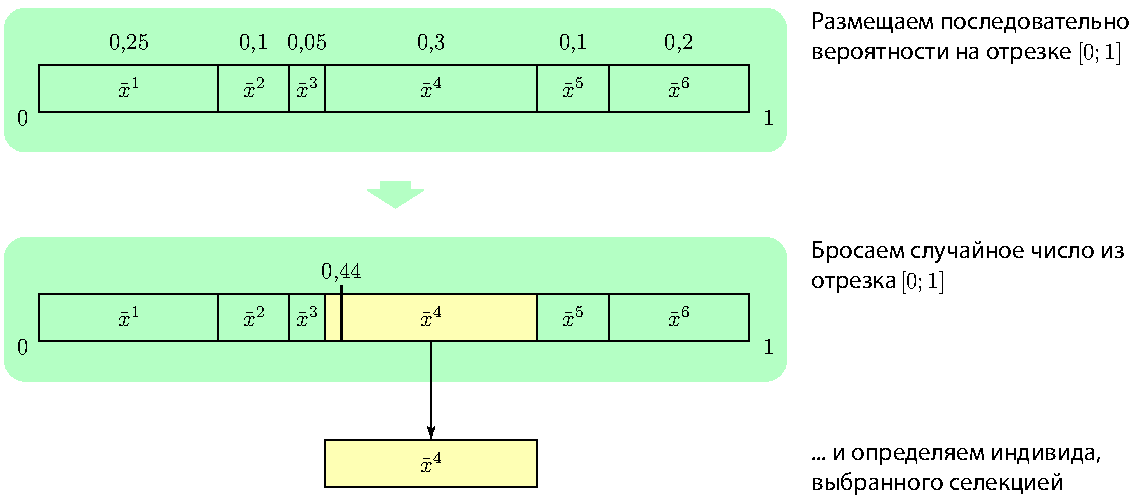
\includegraphics [scale=0.8] {MHL_ProportionalSelection_Sheme}
  \caption{Механизм работы пропорциональной селекции} 
  \label{img:MHL_ProportionalSelection_Sheme}  
\end{figure}

\textbf{Примечание:}

 Использовать реализацию оператора ГА в виде этой функции нецелесообразно ввиду того, что при каждом запуске создается дополнительный массив.  Данная функция аналогична по действию (результат действия аналогичен):
 
 \begin{enumerate}
\item Связке функций MHL\_MakeVectorOfProbabilityForProportionalSelectionV2 и MHL\_ProportionalSelectionV2;
\item Функции MHL\_ProportionalSelectionV3.
 \end{enumerate}
 
Различия по временным затратам на выполнение. У этой реализации самое большое время выполнения.
  
\textbf{Примечание:}

 Под массивом пригодностей понимается специально преобразованный массив значений целевой функции. Процесс подробно описан в стандарте генетического алгоритма. Смотреть здесь. Но это если Вы используете в алгоритмах оптимизации подобных генетическому. а так, если будете использовать, то учитывайте, что массив пригодностей --- это массив вещественных чисел из отрезка $[0;1]$.



\begin{lstlisting}[label=code_use_MHL_ProportionalSelection,caption=Пример использования]
        int i;
        int VMHL_N=10;//Размер массива (число строк)
        double *Fitness;
        Fitness=new double[VMHL_N];
        //Заполним вектор случайными значениями пригодностей индивидов
        //на практике, конечно, пригодности вычисляются, например, в
        //процессе работы ГА
        for (i=0;i<VMHL_N;i++) Fitness[i]=MHL_RandomNumber();

        //Вызов функции
        int Number=MHL_ProportionalSelection(Fitness,VMHL_N);

        //Используем полученный результат

        //Например:
        MHL_ShowVector (Fitness,VMHL_N,"Вектор пригодностей индивидов", "a");
        // Вектор пригодностей индивидов:
        //a =
        //0.368073
        //0.474609
        //0.297089
        //0.373474
        //0.102203
        //0.774292
        //0.487335
        //0.747742
        //0.505646
        //0.901184

        MHL_ShowNumber (Number,"Номер выбранного индивида", "Number");
        //Номер выбранного индивида:
        //Number=5

        delete [] Fitness;
\end{lstlisting}

\subsubsection{MHL\_ProportionalSelectionV2}\label{MHL_ProportionalSelectionV2}

Пропорциональная селекция. Оператор генетического алгоритма. Работает с вектором вероятностей выбора индивидов, который можно получить из вектора пригодностей индивидов посредством функции MHL\_MakeVectorOfProbabilityForProportionalSelectionV2.


\begin{lstlisting}[label=code_syntax_MHL_ProportionalSelectionV2,caption=Синтаксис]
int MHL_ProportionalSelectionV2(double *VectorOfProbability, int VMHL_N);
\end{lstlisting}

\textbf{Входные параметры:}
 
 VectorOfProbability --- массив вероятностей выбора индивидов для порпоциональной селекции;
 
 VMHL\_N --- размер массива пригодностей.

\textbf{Возвращаемое значение:} 

Номер выбранной пригодности, а, соответственно, номер индивида популяции.

 \textbf{Принцип работы:}

\begin{figure} [h]
  \center
  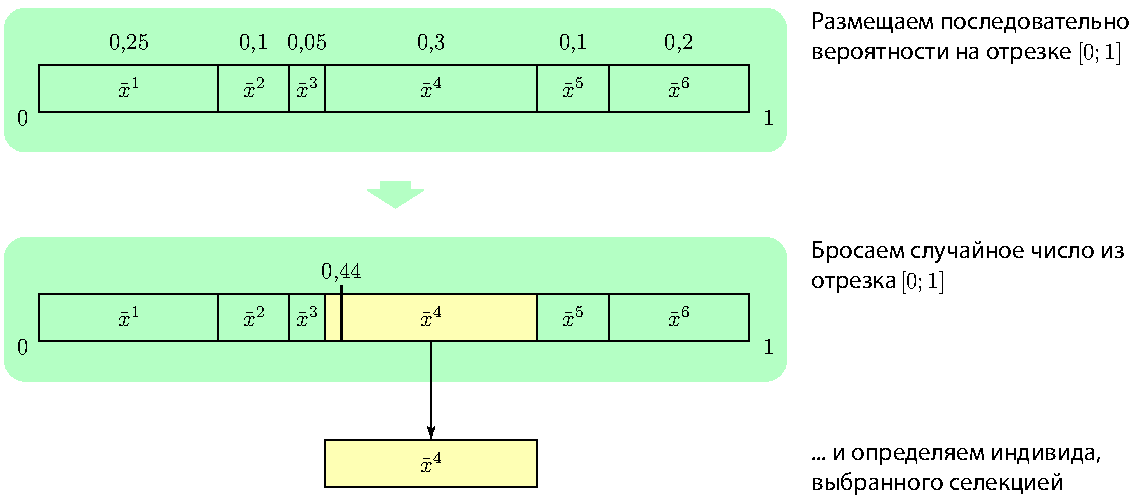
\includegraphics [scale=0.8] {MHL_ProportionalSelection_Sheme}
  \caption{Механизм работы пропорциональной селекции} 
  \label{img:MHL_ProportionalSelection_Sheme}  
\end{figure}

\textbf{Примечание:}

Связка данной функции и MHL\_MakeVectorOfProbabilityForProportionalSelectionV2 аналогична по действию (результат действия аналогичен):
 
 \begin{enumerate}
\item Функции MHL\_ProportionalSelection;
\item Функции MHL\_ProportionalSelectionV3.
 \end{enumerate}
 
 Различия по временным затратам на выполнение. У этой связки выполнение быстрее, чем у MHL\_ProportionalSelection.
  
\textbf{О функции:}

 Данная функция используется в стандартном генетическом алгоритме, реализованным в виде функции MHL\_StandartGeneticAlgorithm. Работает в связке с функцией MHL\_MakeVectorOfProbabilityForProportionalSelectionV2. Оператор селекции работает с массивом пригодностей индивидов, но непосредственно пропорциональная селекция выбирает индивида исходя из вероятностей выбора индивидов. Каждый раз для выбора индивида создавать массив вероятностей затратно, поэтому для каждой популяции на каждом поколении вначале вызывается функция MHL\_MakeVectorProbabilityForSelectionProportionalV2 для генерации вектора вероятностей выбора индивида, а затем этот массив и подставляется в пропорциональную селекцию.




\begin{lstlisting}[label=code_use_MHL_ProportionalSelectionV2,caption=Пример использования]
        int i;
        int VMHL_N=10;//Размер массива (число строк)
        double *Fitness;
        Fitness=new double[VMHL_N];
        //Заполним вектор случайными значениями пригодностей индивидов
        //на практике, конечно, пригодности вычисляются, например, в
        //процессе работы ГА
        for (i=0;i<VMHL_N;i++) Fitness[i]=MHL_RandomNumber();

        //Для работы этого варианта пропорциональной селекции нужен
        //массив вероятностей выбора индивидов для порпоциональной селекции;
        double *VectorProbability;
        VectorProbability=new double[VMHL_N];
        //Сформируем этот массив
        MHL_MakeVectorOfProbabilityForProportionalSelectionV2(Fitness,VectorProbability,VMHL_N);

        //Вызов функции
        int Number=MHL_ProportionalSelectionV2(VectorProbability,VMHL_N);

        //Используем полученный результат
        MHL_ShowVector (Fitness,VMHL_N,"Вектор пригодностей индивидов", "a");
        // Вектор пригодностей индивидов:
        //a =	
        //0.681061
        //0.629517
        //0.697021
        //0.140045
        //0.221649
        //0.203461
        //0.702576
        //0.998077
        //0.853607
        //0.19928

        MHL_ShowVector (VectorProbability,VMHL_N,"Вектор вероятностей выбора индивидов", "VectorProbability");
        // Вектор вероятностей выбора индивидов:
        //VectorProbability =	
        //0.137809
        //0.124679
        //0.141874
        //0
        //0.0207864
        //0.0161534
        //0.143289
        //0.21856
        //0.18176
        //0.0150884

        MHL_ShowNumber (TMHL_SumVector(VectorProbability,VMHL_N),"Его сумма", "Sum");
        // Его сумма:
        //Sum=1
                
        MHL_ShowNumber (Number,"Номер выбранного индивида", "Number");
        
        // Номер выбранного индивида:
        //Number=6
        
        delete [] Fitness;
        delete [] VectorProbability;
\end{lstlisting}

\subsubsection{MHL\_ProportionalSelectionV3}\label{MHL_ProportionalSelectionV3}

Пропорциональная селекция. Оператор генетического алгоритма. Работает с массивом пригодностей (обязательно не отрицательными).


\begin{lstlisting}[label=code_syntax_MHL_ProportionalSelectionV3,caption=Синтаксис]
int MHL_ProportionalSelectionV3(double *Fitness, int VMHL_N);
\end{lstlisting}

\textbf{Входные параметры:}
 
  Fitness --- массив пригодностей (В отличии от MHL\_ProportionalSelection вектор пригодностей должен быть именно вектором пригодностей, то есть все элементы Fitness должны быть больше нуля);
  
 VMHL\_N --- размер массива пригодностей.

\textbf{Возвращаемое значение:} 

Номер выбранной пригодности, а, соответственно, номер индивида популяции.

 \textbf{Принцип работы:}

\begin{figure} [h]
  \center
  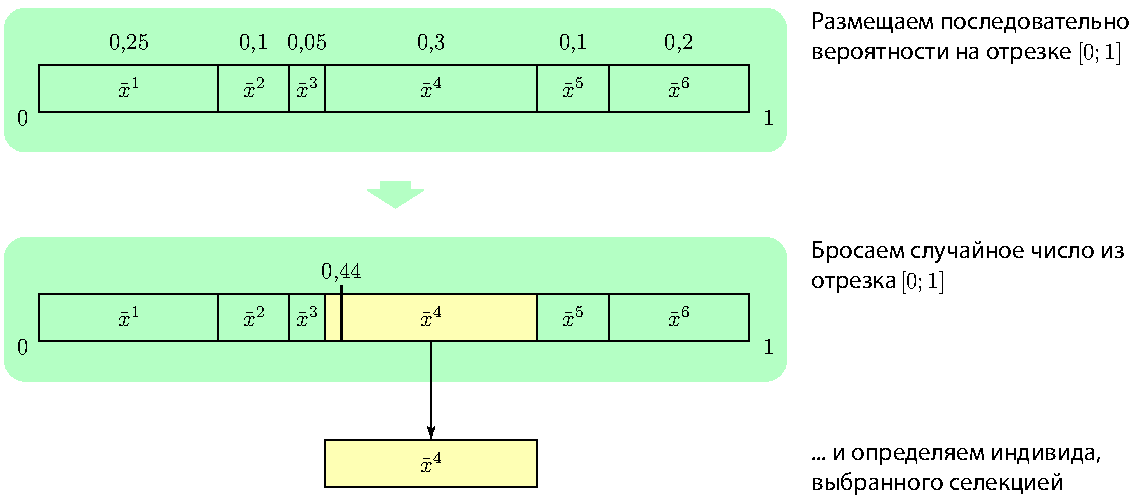
\includegraphics [scale=0.8] {MHL_ProportionalSelection_Sheme}
  \caption{Механизм работы пропорциональной селекции} 
  \label{img:MHL_ProportionalSelection_Sheme}  
\end{figure}

\textbf{Примечание:}

Данная функция аналогична по действию (результат действия аналогичен):
 
 \begin{enumerate}
\item Связке функций MHL\_MakeVectorOfProbabilityForProportionalSelectionV2 и MHL\_ProportionalSelectionV2;
\item Функции MHL\_ProportionalSelection.
 \end{enumerate}
 
 Различия по временным затратам на выполнение. Эта реализация быстрее, чем MHL\_SelectionProportional
 и почти равна связке функций MHL\_MakeVectorOfProbabilityForProportionalSelectionV2 и MHL\_ProportionalSelectionV2,
 но реализация отличается от формульной записи в угоду более простой записи в программировании, но ей тождественна.
  
\textbf{Примечание:}

Под массивом пригодностей понимается специально преобразованный массив значений целевой функции. Процесс подробно описан в стандарте генетического алгоритма. Смотреть здесь. Но это если Вы используете в алгоритмах оптимизации подобных генетическому. а так, если будете использовать, то учитывайте, что массив пригодностей --- это массив вещественных чисел из отрезка $[0;1]$.




\begin{lstlisting}[label=code_use_MHL_ProportionalSelectionV3,caption=Пример использования]
        int i;
        int VMHL_N=10;//Размер массива (число строк)
        double *Fitness;
        Fitness=new double[VMHL_N];
        //Заполним вектор случайными значениями пригодностей индивидов
        //на практике, конечно, пригодности вычисляются, например, в
        //процессе работы ГА
        for (i=0;i<VMHL_N;i++) Fitness[i]=MHL_RandomNumber();

        //Вызов функции
        int Number=MHL_ProportionalSelectionV3(Fitness,VMHL_N);

        //Используем полученный результат
        MHL_ShowVector (Fitness,VMHL_N,"Вектор пригодностей индивидов", "a");
        // Вектор пригодностей индивидов:
        //a =	
        //0.774231
        //0.15918
        //0.671448
        //0.0546265
        //0.881012
        //0.766541
        //0.638275
        //0.0705261
        //0.234528
        //0.0510559

        MHL_ShowNumber (Number,"Номер выбранного индивида", "Number");
        // Номер выбранного индивида:
        //Number=0
        
        delete [] Fitness;
\end{lstlisting}

\subsubsection{MHL\_RankSelection}\label{MHL_RankSelection}

Ранговая селекция. Оператор генетического алгоритма. Работает с вектором вероятностей выбора индивидов, который можно получить из вектора пригодностей индивидов посредством функции MHL\_MakeVectorOfRankForRankSelection (для получения массива рангов) и потом функции MHL\_MakeVectorOfProbabilityForProportionalSelectionV2 (для получения массива вероятностей выбора индивидов по рангам).


\begin{lstlisting}[label=code_syntax_MHL_RankSelection,caption=Синтаксис]
int MHL_RankSelection(double *VectorOfProbability, int VMHL_N);
\end{lstlisting}

\textbf{Входные параметры:}
 
 VectorOfProbability --- массив вероятностей выбора индивидов для ранговой селекции;
 
 VMHL\_N --- размер массива VectorProbability.

\textbf{Возвращаемое значение:} 

 Номер выбранного индивида популяции.

 \textbf{Принцип работы:}

\begin{figure} [h]
  \center
  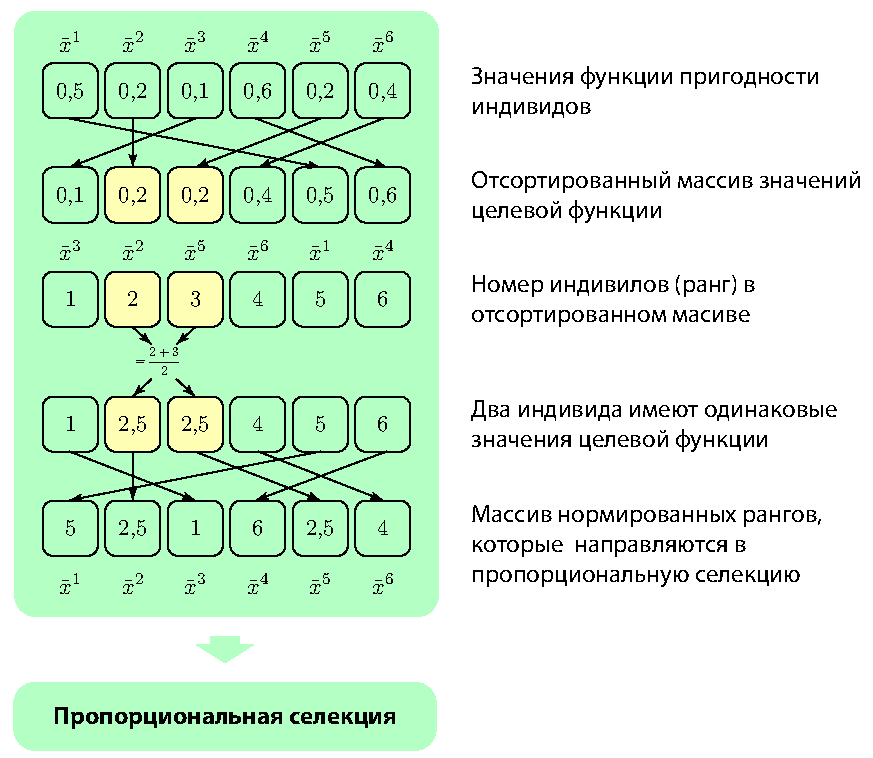
\includegraphics [scale=0.8] {MHL_RankSelection_Sheme}
  \caption{Механизм работы ранговой селекции} 
  \label{img:MHL_RankSelection_Sheme}  
\end{figure}

\textbf{О функции:}

Данная функция используется в стандартном генетическом алгоритме, реализованным в виде функции MHL\_StandartGeneticAlgorithm. Работает в связке с функциями MHL\_MakeVectorOfRankForRankSelection и MHL\_MakeVectorOfProbabilityForProportionalSelectionV2. Оператор селекции работает с массивом пригодностей индивидов, но непосредственно ранговая селекция выбирает индивида исходя из рангов индивидов, преобразованных в вероятности выбора. Каждый раз для выбора индивида создавать массив вероятностей и рангов затратно, поэтому для каждой популяции на каждом поколении вначале вызывается функция MHL\_MakeVectorOfRankForRankSelection для генерации вектора рангов, а затем MHL\_MakeVectorOfProbabilityForProportionalSelectionV2 для генерации вектора вероятностей выбора индивида, а затем этот массив и подставляется в ранговую селекцию.
  
\textbf{Примечание:}

На рисунке показано, что ранги подаются в пропорциональную селекцию, но из кода этого не видно. Но по своей сути код данной функции повторяет код функции MHL\_ProportionalSelectionV2 и также требует вектор вероятностей выбора. Так что всё соответствует рисунку.




\begin{lstlisting}[label=code_use_MHL_RankSelection,caption=Пример использования]
        int i;
        int VMHL_N=7;//Размер массива
        double *Fitness;
        Fitness=new double[VMHL_N];
        for (i=0;i<VMHL_N;i++)
         Fitness[i]=MHL_RandomUniformInt(1,10)/10.;

        double *Rank;
        Rank=new double[VMHL_N];

        double *VectorProbability;
        VectorProbability=new double[VMHL_N];

        //Сформируем вектор рангов
        MHL_MakeVectorOfRankForRankSelection(Fitness,Rank,VMHL_N);
        //Из вектора рангов получим вектор вероятностей выбора
        MHL_MakeVectorOfProbabilityForProportionalSelectionV2(Rank,VectorProbability,VMHL_N);

        //Вызов функции
        int Number=MHL_RankSelection(VectorProbability,VMHL_N);

        //Используем полученный результат

        MHL_ShowVector (Fitness,VMHL_N,"Массив пригодностей", "Fitness");
        // Массив пригодностей:
        //Fitness =	
        //0.2
        //0.2
        //0.6
        //0.8
        //0.4
        //0.3
        //0.2

        MHL_ShowVector (Rank,VMHL_N,"Массив рангов", "Rank");
        // Массив рангов:
        //Rank =	
        //2
        //2
        //6
        //7
        //5
        //4
        //2

        MHL_ShowVector (VectorProbability,VMHL_N,"Массив вероятностей выбора", "VectorProbability");
        //Массив вероятностей выбора:
        //VectorProbability =	
        //0
        //0
        //0.285714
        //0.357143
        //0.214286
        //0.142857
        //0

        MHL_ShowNumber (Number,"Номер выбранного индивида", "Number");
        // Номер выбранного индивида:
        //Number=3

        delete [] Fitness;
        delete [] Rank;
        delete [] VectorProbability;
\end{lstlisting}

\subsubsection{MHL\_SelectItemOnProbability}\label{MHL_SelectItemOnProbability}

Функция выбирает случайно номер элемента из вектора, где вероятность выбора каждого элемента определяется значением в векторе P.


\begin{lstlisting}[label=code_syntax_MHL_SelectItemOnProbability,caption=Синтаксис]
int MHL_SelectItemOnProbability(double *P, int VMHL_N);
\end{lstlisting}

\textbf{Входные параметры:}
 
 P --- вектор вероятностей выбора каждого элемента, то есть его компоненты должны быть из отрезка $[0;1]$, а сумма их равна 1;
 
 VMHL\_N --- размер вектора.

\textbf{Возвращаемое значение:} 

Номер выбранного элемента.

\textbf{Примечание:}

 Проверка на правильность вектора P не проводится, так как функция обычно вызывается многократно, а проводить постоянно проверку накладно. Всё на Вашей совести.



\begin{lstlisting}[label=code_use_MHL_SelectItemOnProbability,caption=Пример использования]
        int VMHL_N=10;//Размер массива (число строк)
        double *a;
        a=new double[VMHL_N];
        //Заполним вектор случайными значениями вероятностей
        MHL_RandomVectorOfProbability(a, VMHL_N);

        //Вызов функции
        int Number=MHL_SelectItemOnProbability(a,VMHL_N);

        //Используем полученный результат
        MHL_ShowVector (a,VMHL_N,"Вектор вероятностей выбора", "a");
        // Вектор вероятностей выбора:
        //Вектор вероятностей выбора:
        //a =
        //0.0701006
        //0.190423
        //0.0231631
        //0.160255
        //0.0983935
        //0.038739
        //0.166252
        //0.105259
        //0.0621408
        //0.0852747

        MHL_ShowNumber (Number,"Номер выбранного элемента", "Number");
        // Номер выбранного элемента:
        //Number=6

        delete [] a;
\end{lstlisting}

\subsubsection{MHL\_StandartBinaryGeneticAlgorithm}\label{MHL_StandartBinaryGeneticAlgorithm}

Стандартный генетический алгоритм на бинарных строках. Реализация алгоритма из документа <<Генетический алгоритм. Стандарт. v.3.0>>.


\begin{lstlisting}[label=code_syntax_MHL_StandartBinaryGeneticAlgorithm,caption=Синтаксис]
int MHL_StandartBinaryGeneticAlgorithm(int *Parameters, double (*FitnessFunction)(int*,int), int *VMHL_ResultVector, double *VMHL_Result);
\end{lstlisting}

\textbf{Входные параметры:}
 
Parameters --- Вектор параметров генетического алгоритма. Каждый элемент обозначает свой параметр:
 
 \begin{itemize}
 \item [0] --- длина бинарной хромосомы (определяется задачей оптимизации, что мы решаем);
 
 \item [1] --- число вычислений целевой функции (CountOfFitness);
 
 \item [2] --- тип селекции (TypeOfSel):
 
 \begin{itemize}
       \item 0 --- ProportionalSelection (Пропорциональная селекция);
 
       \item 1 --- RankSelection (Ранговая селекция);
 
       \item 2 --- TournamentSelection (Турнирная селекция).
	    \end{itemize}
 
 \item [3] --- тип скрещивания (TypeOfCros):
  \begin{itemize}
       \item 0 --- SinglepointCrossover (Одноточечное скрещивание);
 
       \item 1 --- TwopointCrossover (Двуточечное скрещивание);
 
       \item 2 --- UniformCrossover (Равномерное скрещивание).
	    \end{itemize}
 
 \item [4] --- тип мутации (TypeOfMutation):
  \begin{itemize}
       \item 0 --- Weak (Слабая мутация);
 
       \item 1 --- Average (Средняя мутация);
 
       \item 2 --- Strong (Сильная мутация).
	    \end{itemize}
 
 \item [5] --- тип формирования нового поколения (TypeOfForm):
  \begin{itemize}
       \item 0 --- OnlyOffspringGenerationForming (Только потомки);
 
       \item 1 --- OnlyOffspringWithBestGenerationForming (Только потомки и копия лучшего индивида).
	    \end{itemize}
 \end{itemize}
 
FitnessFunction --- указатель на целевую функцию (если решается задача условной оптимизации, то учет ограничений должен быть включен в эту функцию);
 
VMHL\_ResultVector --- найденное решение (бинарный вектор);
 
VMHL\_Result --- значение целевой функции в точке, определенной вектором VMHL\_ResultVector.

\textbf{Возвращаемое значение:} 

 1 --- завершил работу без ошибок. Всё хорошо.
 
 0 --- возникли при работе ошибки. Скорее всего в этом случае в VMHL\_ResultVector и в VMHL\_Result не содержится решение задачи.

 \textbf{Принцип работы} смотрите ниже на рисунке \ref{img:MHL_StandartBinaryGeneticAlgorithm_Sheme} на странице \pageref{img:MHL_StandartBinaryGeneticAlgorithm_Sheme}.

\begin{figure} [h]
  \center
  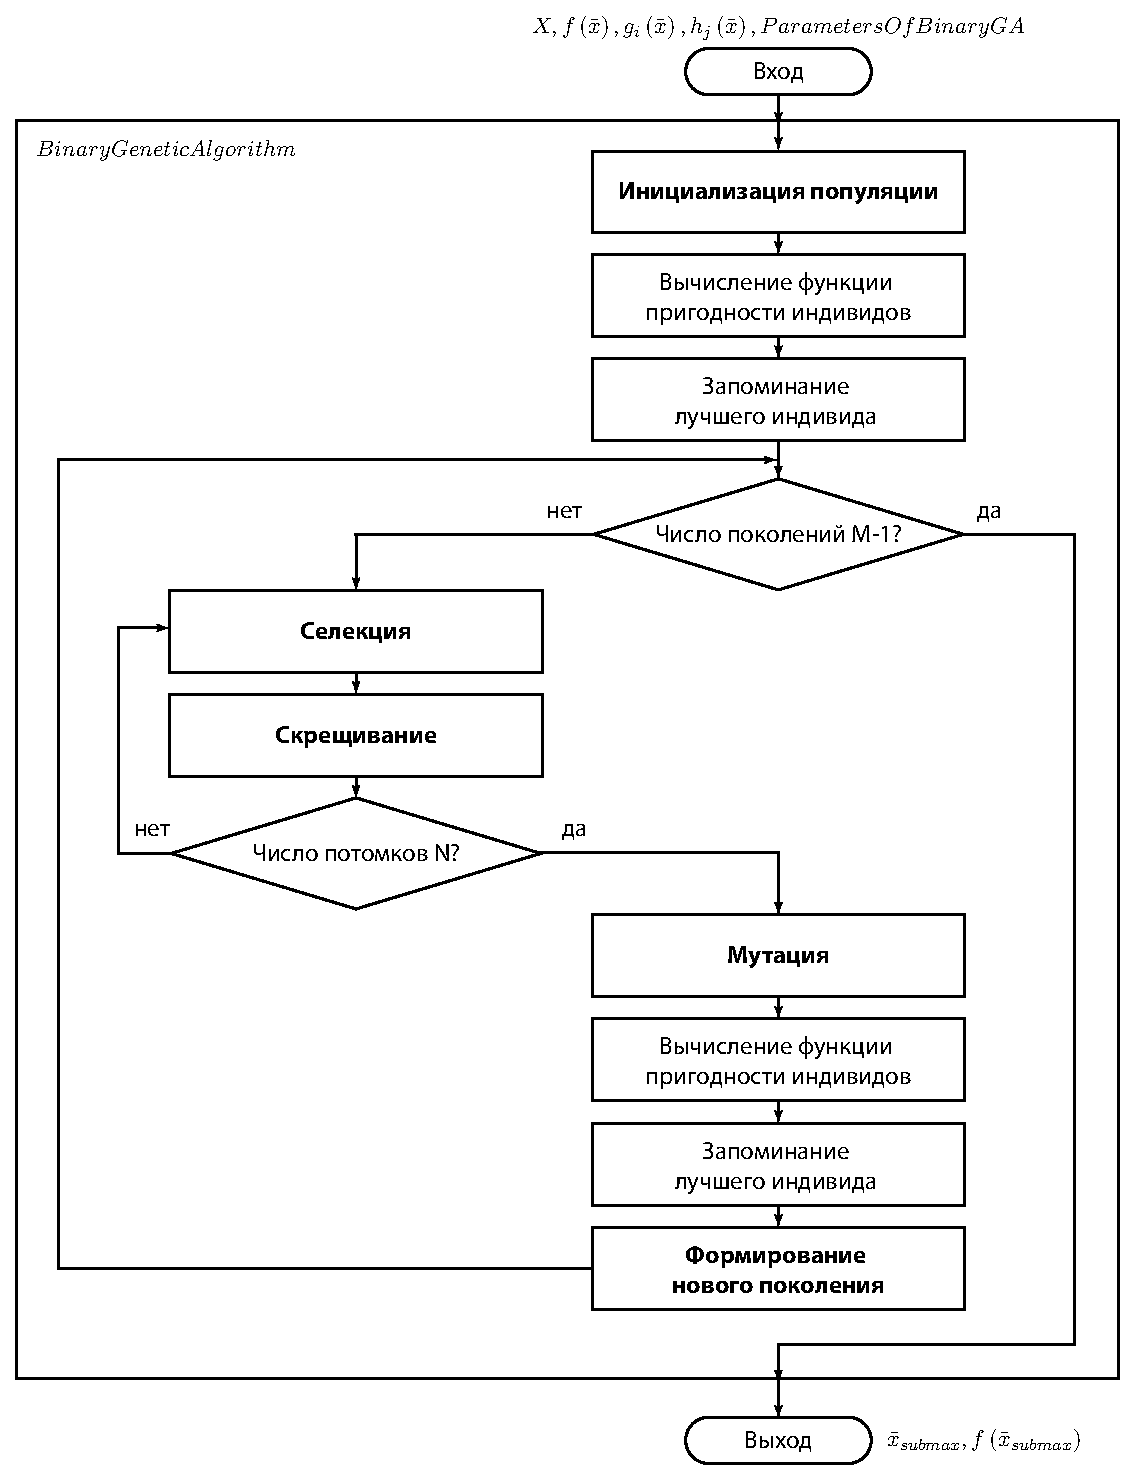
\includegraphics [scale=0.5] {MHL_StandartBinaryGeneticAlgorithm_Sheme}
  \caption{Механизм работы генетического алгоритма} 
  \label{img:MHL_StandartBinaryGeneticAlgorithm_Sheme}  
\end{figure}

\textbf{О функции:}

Реализация алгоритма из документа <<Генетический алгоритм. Стандарт. v.3.0>>.

\href{https://github.com/Harrix/Standard-Genetic-Algorithm}{https://github.com/Harrix/Standard-Genetic-Algorithm}

Алгоритм бинарной оптимизации. Ищет максимум целевой функции FitnessFunction.

Решением является бинарная строка, то есть вектор, состоящий из 0 и 1.

\textbf{Примерный настройки} (для примера Вы можете поставить такие рабочие настройки):

 Parameters[0]=50;
 
Parameters[1]=100*100;

Parameters[2]=2;

Parameters[3]=2;

Parameters[4]=1;

Parameters[5]=1;


\textbf{Примечание:}

 На рисунке блок-схемы сГА на бинарных строках число поколений обозначено буквой \textbf{M}, в коде функции же обозначается переменной \textbf{NumberOfGenerations}.


\textbf{Примечание:}

 В сГА на бинарных строках не нужно задавать в параметрах число поколений и размер популяции, а только число вычислений целевой функции. Почему? Алгоритм сам определит число поколений и размер популяции, исходя из принципа, что число поколений и размер популяции должны быть примерно равны. Поэтому выбирайте значение Parameters[1] в виде:

int K=100;

Parameters[1]=K*K;

То есть в виде квадрата целого числа. В противном случае реальное число вычислений целевой функции и значение Parameters[1] будут не совпадать.

Код целевой функции:
\begin{lstlisting}[caption=Оптимизируемая функция]
double Func(int *x,int VMHL_N)
{
//Сумма всех элементов массива
return TMHL_SumVector(x,VMHL_N);
}
//---------------------------------------------------------------------------
\end{lstlisting}


\begin{lstlisting}[label=code_use_MHL_StandartBinaryGeneticAlgorithm,caption=Пример использования]
        int ChromosomeLength=50;//Длина хромосомы
        int CountOfFitness=50*50;//Число вычислений целевой функции
        int TypeOfSel=1;//Тип селекции
        int TypeOfCros=0;//Тип скрещивания
        int TypeOfMutation=1;//Тип мутации
        int TypeOfForm=0;//Тип формирования нового поколения

        int *ParametersOfStandartBinaryGeneticAlgorithm;
        ParametersOfStandartBinaryGeneticAlgorithm=new int[6];
        ParametersOfStandartBinaryGeneticAlgorithm[0]=ChromosomeLength;//Длина хромосомы
        ParametersOfStandartBinaryGeneticAlgorithm[1]=CountOfFitness;//Число вычислений целевой функции
        ParametersOfStandartBinaryGeneticAlgorithm[2]=TypeOfSel;//Тип селекции
        ParametersOfStandartBinaryGeneticAlgorithm[3]=TypeOfCros;//Тип скрещивания
        ParametersOfStandartBinaryGeneticAlgorithm[4]=TypeOfMutation;//Тип мутации
        ParametersOfStandartBinaryGeneticAlgorithm[5]=TypeOfForm;//Тип формирования нового поколения

        int *Decision;//бинарное решение
        Decision=new int[ChromosomeLength];
        double ValueOfFitnessFunction;//значение функции пригодности в точке Decision
        int VMHL_Success=0;//Успешен ли будет запуск cГА

        //Запуск алгоритма
        VMHL_Success=MHL_StandartBinaryGeneticAlgorithm (ParametersOfStandartBinaryGeneticAlgorithm,Func, Decision, &ValueOfFitnessFunction);

        //Используем полученный результат
        MHL_ShowNumber(VMHL_Success,"Как прошел запуск","VMHL_Success");
        //Как прошел запуск:
        //VMHL_Success=1

        if (VMHL_Success==1)
         {
         MHL_ShowVectorT(Decision,ChromosomeLength,"Найденное решение","Decision");
         //Найденное решение:
         //Decision =
         //1	1	1	1	1	1	1	1	1	1	1	1	1	1	1	1	1	1	1	1	1	1	1	1	1	1	1	1	1	1	1	1	1	1	1	1	1	1	1	1	1	1	1	1	1	1	1	1	1	1

         MHL_ShowNumber(ValueOfFitnessFunction,"Значение функции пригодности","ValueOfFitnessFunction");
         // Значение функции пригодности:
         //ValueOfFitnessFunction=50
         }

        delete [] ParametersOfStandartBinaryGeneticAlgorithm;
        delete [] Decision;
\end{lstlisting}

\subsubsection{MHL\_StandartGeneticAlgorithm}\label{MHL_StandartGeneticAlgorithm}

Стандартный генетический алгоритм на бинарных и вещественных строках. Реализация алгоритма из документа <<Генетический алгоритм. Стандарт. v.3.0>>.


\begin{lstlisting}[label=code_syntax_MHL_StandartGeneticAlgorithm,caption=Синтаксис]
int MHL_StandartGeneticAlgorithm(int *Parameters, int *NumberOfParts, double *Left, double *Right, double (*FitnessFunction)(double*,int), double *VMHL_ResultVector, double *VMHL_Result);
int MHL_StandartGeneticAlgorithm(int *Parameters, double (*FitnessFunction)(int*,int), int *VMHL_ResultVector, double *VMHL_Result);
\end{lstlisting}

Функция и функция перегрузка вызывают функции MHL\_StandartBinaryGeneticAlgorithm и  MHL\_StandartRealGeneticAlgorithm.

\textbf{Принцип работы:}

\begin{figure} [h]
  \center
  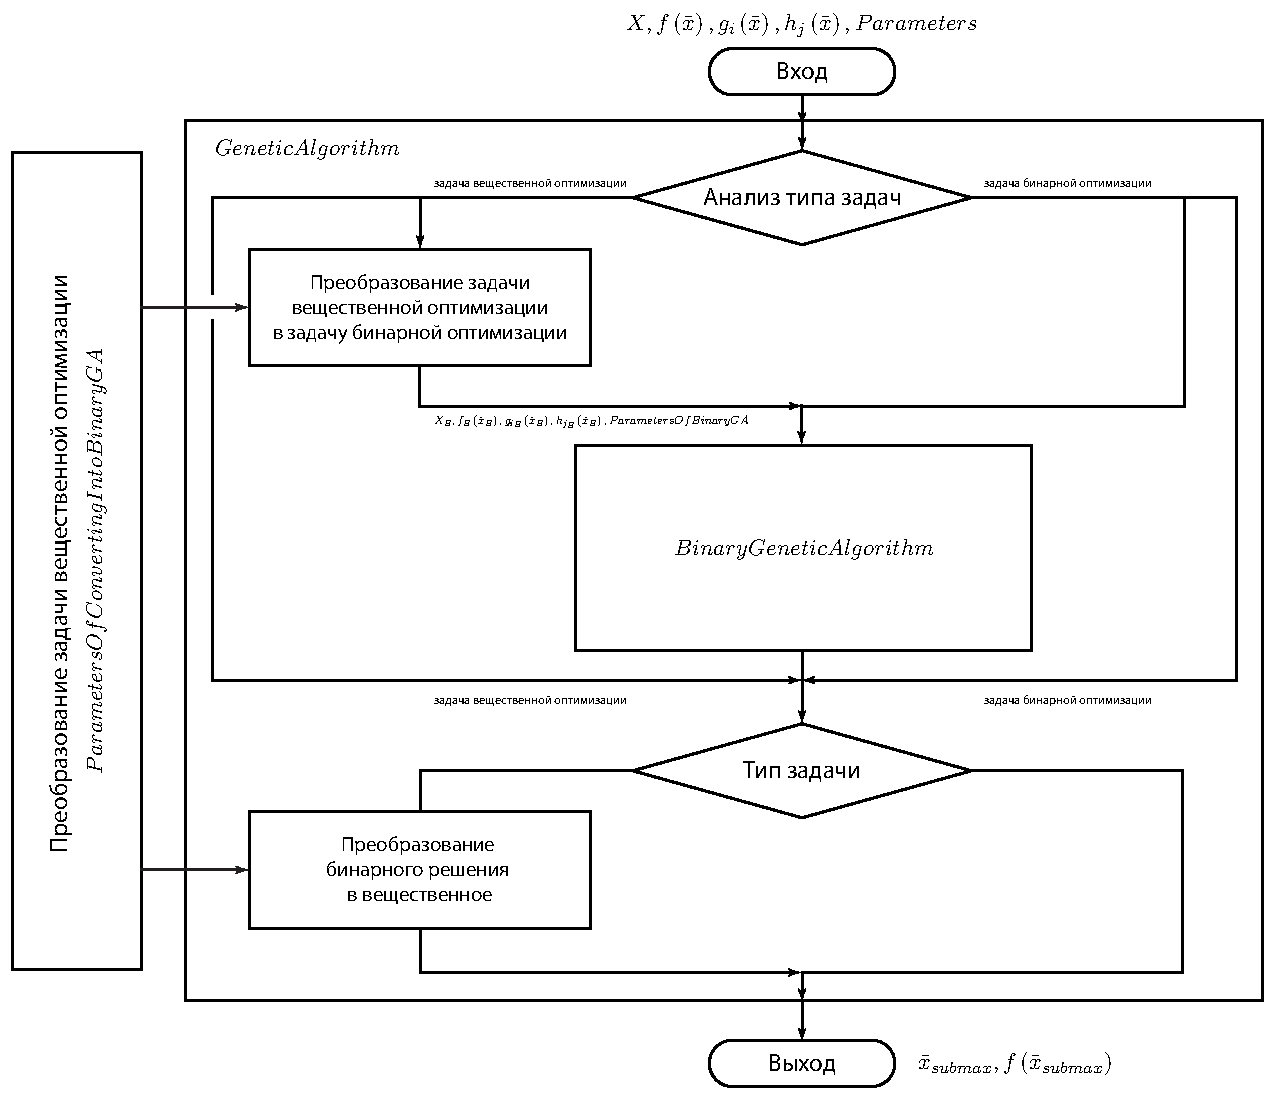
\includegraphics [scale=0.5] {MHL_StandartGeneticAlgorithm_Sheme}
  \caption{Механизм работы генетического алгоритма} 
\end{figure}

\textbf{Входные параметры:}
 
Parameters --- Вектор параметров генетического алгоритма. Каждый элемент обозначает свой параметр:
 
 \begin{itemize}
 \item [0] --- длина бинарной хромосомы (определяется задачей оптимизации, что мы решаем);
 
 \item [1] --- число вычислений целевой функции (CountOfFitness);
 
 \item [2] --- тип селекции (TypeOfSel):
 
 \begin{itemize}
       \item 0 --- ProportionalSelection (Пропорциональная селекция);
 
       \item 1 --- RankSelection (Ранговая селекция);
 
       \item 2 --- TournamentSelection (Турнирная селекция).
	    \end{itemize}
 
 \item [3] --- тип скрещивания (TypeOfCros):
  \begin{itemize}
       \item 0 --- SinglepointCrossover (Одноточечное скрещивание);
 
       \item 1 --- TwopointCrossover (Двуточечное скрещивание);
 
       \item 2 --- UniformCrossover (Равномерное скрещивание).
	    \end{itemize}
 
 \item [4] --- тип мутации (TypeOfMutation):
  \begin{itemize}
       \item 0 --- Weak (Слабая мутация);
 
       \item 1 --- Average (Средняя мутация);
 
       \item 2 --- Strong (Сильная мутация).
	    \end{itemize}
 
 \item [5] --- тип формирования нового поколения (TypeOfForm):
  \begin{itemize}
       \item 0 --- OnlyOffspringGenerationForming (Только потомки);
 
       \item 1 --- OnlyOffspringWithBestGenerationForming (Только потомки и копия лучшего индивида).
	    \end{itemize}
 \end{itemize}
 
FitnessFunction --- указатель на целевую функцию (если решается задача условной оптимизации, то учет ограничений должен быть включен в эту функцию);
 
VMHL\_ResultVector --- найденное решение (бинарный вектор);
 
VMHL\_Result --- значение целевой функции в точке, определенной вектором VMHL\_ResultVector.

\textbf{Возвращаемое значение:} 

 1 --- завершил работу без ошибок. Всё хорошо.
 
 0 --- возникли при работе ошибки. Скорее всего в этом случае в VMHL\_ResultVector и в VMHL\_Result не содержится решение задачи.

 \textbf{Принцип работы} смотрите ниже на рисунке \ref{img:MHL_StandartBinaryGeneticAlgorithm_Sheme} на странице \pageref{img:MHL_StandartBinaryGeneticAlgorithm_Sheme}.

\begin{figure} [h]
  \center
  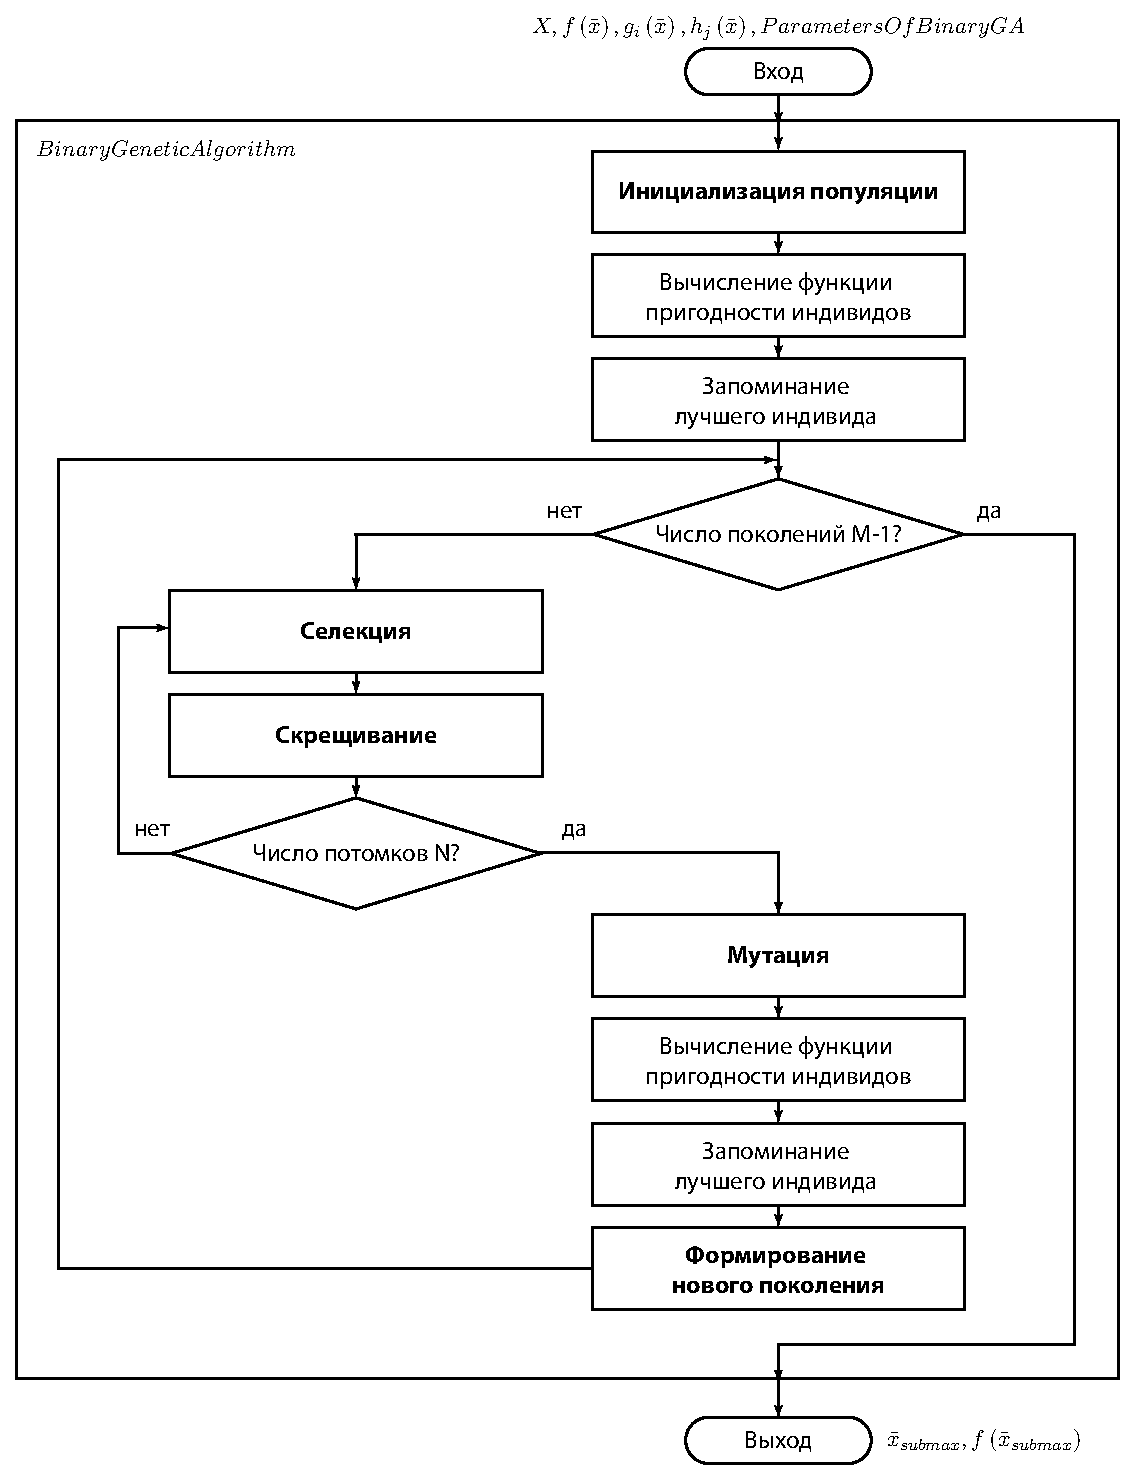
\includegraphics [scale=0.5] {MHL_StandartBinaryGeneticAlgorithm_Sheme}
  \caption{Механизм работы генетического алгоритма} 
\end{figure}

\textbf{О функции:}

Реализация алгоритма из документа <<Генетический алгоритм. Стандарт. v.3.0>>.

\href{https://github.com/Harrix/Standard-Genetic-Algorithm}{https://github.com/Harrix/Standard-Genetic-Algorithm}

Алгоритм бинарной оптимизации. Ищет максимум целевой функции FitnessFunction.

Решением является бинарная строка, то есть вектор, состоящий из 0 и 1.

\textbf{Примерный настройки} (для примера Вы можете поставить такие рабочие настройки):

 Parameters[0]=50;
 
Parameters[1]=100*100;

Parameters[2]=2;

Parameters[3]=2;

Parameters[4]=1;

Parameters[5]=1;


\textbf{Примечание:}

 На рисунке блок-схемы сГА на бинарных строках число поколений обозначено буквой \textbf{M}, в коде функции же обозначается переменной \textbf{NumberOfGenerations}.


\textbf{Примечание:}

 В сГА на бинарных строках не нужно задавать в параметрах число поколений и размер популяции, а только число вычислений целевой функции. Почему? Алгоритм сам определит число поколений и размер популяции, исходя из принципа, что число поколений и размер популяции должны быть примерно равны. Поэтому выбирайте значение Parameters[1] в виде:

int K=100;

Parameters[1]=K*K;

То есть в виде квадрата целого числа. В противном случае реальное число вычислений целевой функции и значение Parameters[1] будут не совпадать.

Код целевой функции:
\begin{lstlisting}[caption=Оптимизируемая функция]
double Func(int *x,int VMHL_N)
{
//Сумма всех элементов массива
return TMHL_SumVector(x,VMHL_N);
}
//---------------------------------------------------------------------------
\end{lstlisting}

\textbf{Для переопределенной функции.}

\textbf{Входные параметры:}
 
Parameters --- Вектор параметров генетического алгоритма. Каждый элемент обозначает свой параметр:
 
 \begin{itemize}
 \item   [0] --- длина вещественной хромосомы (определяется задачей оптимизации, что мы решаем);
  \item   [1] --- число вычислений целевой функции (CountOfFitness);
  \item    [2] --- тип селекции (TypeOfSel):
 \begin{itemize}
       \item 0 --- ProportionalSelection (Пропорциональная селекция);
 
       \item 1 --- RankSelection (Ранговая селекция);
 
       \item 2 --- TournamentSelection (Турнирная селекция).
	    \end{itemize}
 
 \item [3] --- тип скрещивания (TypeOfCros):
  \begin{itemize}
       \item 0 --- SinglepointCrossover (Одноточечное скрещивание);
 
       \item 1 --- TwopointCrossover (Двуточечное скрещивание);
 
       \item 2 --- UniformCrossover (Равномерное скрещивание).
	    \end{itemize}
 
 \item [4] --- тип мутации (TypeOfMutation):
  \begin{itemize}
       \item 0 --- Weak (Слабая мутация);
 
       \item 1 --- Average (Средняя мутация);
 
       \item 2 --- Strong (Сильная мутация).
	    \end{itemize}
 
 \item [5] --- тип формирования нового поколения (TypeOfForm):
  \begin{itemize}
       \item 0 --- OnlyOffspringGenerationForming (Только потомки);
 
       \item 1 --- OnlyOffspringWithBestGenerationForming (Только потомки и копия лучшего индивида).
	    \end{itemize}
 \item [6] --- тип преобразования задачи вещественной оптимизации в задачу бинарной оптимизации (TypOfConverting);
   \begin{itemize}
        \item 0 --- IntConverting (Стандартное представление целого числа –-- номер узла в сетке дискретизации);
        \item 1 --- GrayСodeConverting (Стандартный рефлексивный Грей-код).
			    \end{itemize}
 \end{itemize}
 
 NumberOfParts --- указатель на массив: на сколько частей делить каждую вещественную координату при дискретизации (размерность Parameters[0]);
 
  Желательно брать по формуле $NumberOfParts[i]=2^k-1$, где $k$ --- натуральное число, например, 12.
  
 Left --- массив левых границ изменения каждой вещественной координаты (размерность Parameters[0]);
 
 Right --- массив правых границ изменения каждой вещественной координаты (размерность Parameters[0]);
 
 FitnessFunction --- указатель на целевую функцию (если решается задача условной оптимизации, то учет ограничений должен быть включен в эту функцию);
 
 VMHL\_ResultVector --- найденное решение (вещественный вектор);
 
 VMHL\_Result --- значение целевой функции в точке, определенной вектором VMHL\_ResultVector.

\textbf{Возвращаемое значение:} 

 1 --- завершил работу без ошибок. Всё хорошо.
 
 0 --- возникли при работе ошибки. Скорее всего в этом случае в VMHL\_ResultVector и в VMHL\_Result не содержится решение задачи.

\textbf{О функции:}

Реализация алгоритма из документа <<Генетический алгоритм. Стандарт. v.3.0>>.

\href{https://github.com/Harrix/Standard-Genetic-Algorithm}{https://github.com/Harrix/Standard-Genetic-Algorithm}

Алгоритм вещественной оптимизации. Ищет максимум целевой функции FitnessFunction.

Решением является бинарная строка, то есть вектор, состоящий из 0 и 1.

\textbf{Примерный настройки} (для примера Вы можете поставить такие рабочие настройки):

 Parameters[0]=50;
 
Parameters[1]=100*100;

Parameters[2]=2;

Parameters[3]=2;

Parameters[4]=1;

Parameters[5]=1;

Parameters[5]=0;


\textbf{Примечание:}

 В сГА на вещественных строках не нужно задавать в параметрах число поколений и размер популяции, а только число вычислений целевой функции. Почему? Алгоритм сам определит число поколений и размер популяции, исходя из принципа, что число поколений и размер популяции должны быть примерно равны. Поэтому выбирайте значение Parameters[1] в виде:

int K=100;

Parameters[1]=K*K;

То есть в виде квадрата целого числа. В противном случае реальное число вычислений целевой функции и значение Parameters[1] будут не совпадать.

Код целевой функции:
\begin{lstlisting}[caption=Оптимизируемая функция]
double Func2(double *x,int VMHL_N)
{
return -((x[0]-2)*(x[0]-2)+(x[1]-2)*(x[1]-2));
}
\end{lstlisting}


\begin{lstlisting}[label=code_use_MHL_StandartGeneticAlgorithm,caption=Пример использования]
        int ChromosomeLength=50;//Длина хромосомы
        int CountOfFitness=50*50;//Число вычислений целевой функции
        int TypeOfSel=1;//Тип селекции
        int TypeOfCros=0;//Тип скрещивания
        int TypeOfMutation=1;//Тип мутации
        int TypeOfForm=0;//Тип формирования нового поколения

        int *ParametersOfStandartBinaryGeneticAlgorithm;
        ParametersOfStandartBinaryGeneticAlgorithm=new int[6];
        ParametersOfStandartBinaryGeneticAlgorithm[0]=ChromosomeLength;//Длина хромосомы
        ParametersOfStandartBinaryGeneticAlgorithm[1]=CountOfFitness;//Число вычислений целевой функции
        ParametersOfStandartBinaryGeneticAlgorithm[2]=TypeOfSel;//Тип селекции
        ParametersOfStandartBinaryGeneticAlgorithm[3]=TypeOfCros;//Тип скрещивания
        ParametersOfStandartBinaryGeneticAlgorithm[4]=TypeOfMutation;//Тип мутации
        ParametersOfStandartBinaryGeneticAlgorithm[5]=TypeOfForm;//Тип формирования нового поколения

        int *Decision;//бинарное решение
        Decision=new int[ChromosomeLength];
        double ValueOfFitnessFunction;//значение функции пригодности в точке Decision
        int VMHL_Success=0;//Успешен ли будет запуск cГА

        //Запуск алгоритма
        VMHL_Success=MHL_StandartGeneticAlgorithm (ParametersOfStandartBinaryGeneticAlgorithm,Func, Decision, &ValueOfFitnessFunction);

        //Используем полученный результат
        MHL_ShowNumber(VMHL_Success,"Как прошел запуск","VMHL_Success");
        //Как прошел запуск:
        //VMHL_Success=1

        if (VMHL_Success==1)
         {
         MHL_ShowVectorT(Decision,ChromosomeLength,"Найденное решение","Decision");
         //Найденное решение:
         //Decision =
         //1	1	1	1	1	1	1	1	1	1	1	1	1	1	1	1	1	1	1	1	1	1	1	1	1	1	1	1	1	1	1	1	1	1	1	1	1	1	1	1	1	1	1	1	1	1	1	1	1	1

         MHL_ShowNumber(ValueOfFitnessFunction,"Значение функции пригодности","ValueOfFitnessFunction");
         // Значение функции пригодности:
         //ValueOfFitnessFunction=50
         }

        delete [] ParametersOfStandartBinaryGeneticAlgorithm;
        delete [] Decision;

        //Для переопределенной функции
        {//чтобы не удалять объявления переменных, заключим в скобки
            int ChromosomeLength=2;//Длина хромосомы
            int CountOfFitness=50*50;//Число вычислений целевой функции
            int TypeOfSel=1;//Тип селекции
            int TypeOfCros=0;//Тип скрещивания
            int TypeOfMutation=1;//Тип мутации
            int TypeOfForm=0;//Тип формирования нового поколения

            int *ParametersOfStandartRealGeneticAlgorithm;
            ParametersOfStandartRealGeneticAlgorithm=new int[7];
            ParametersOfStandartRealGeneticAlgorithm[0]=ChromosomeLength;//Длина хромосомы
            ParametersOfStandartRealGeneticAlgorithm[1]=CountOfFitness;//Число вычислений целевой функции
            ParametersOfStandartRealGeneticAlgorithm[2]=TypeOfSel;//Тип селекции
            ParametersOfStandartRealGeneticAlgorithm[3]=TypeOfCros;//Тип скрещивания
            ParametersOfStandartRealGeneticAlgorithm[4]=TypeOfMutation;//Тип мутации
            ParametersOfStandartRealGeneticAlgorithm[5]=TypeOfForm;//Тип формирования нового поколения
            ParametersOfStandartRealGeneticAlgorithm[6]=0;//Тип формирования нового поколения

            double *Left;//массив левых границ изменения каждой вещественной координаты
            Left=new double[ChromosomeLength];
            double *Right;//массив правых границ изменения каждой вещественной координаты
            Right=new double[ChromosomeLength];
            int *NumberOfParts;//на сколько делить каждую координату
            NumberOfParts=new int[ChromosomeLength];

            //Заполним массивы
            //Причем по каждой коодинтате одинаковые значения выставим
            TMHL_FillVector(Left,ChromosomeLength,-5.);//Пусть будет интервал [-3;3]
            TMHL_FillVector(Right,ChromosomeLength,5.);
            TMHL_FillVector(NumberOfParts,ChromosomeLength,TMHL_PowerOf(2,15)-1);//Делим на 32768-1 частей каждую вещественную координату

            double *Decision;//вещественное решение
            Decision=new double[ChromosomeLength];
            double ValueOfFitnessFunction;//значение целевой функции в точке Decision
            int VMHL_Success=0;//Успешен ли будет запуск cГА

            //Запуск алгоритма
            VMHL_Success=MHL_StandartGeneticAlgorithm (ParametersOfStandartRealGeneticAlgorithm,NumberOfParts,Left,Right,Func2, Decision, &ValueOfFitnessFunction);

            //Используем полученный результат
            MHL_ShowNumber(VMHL_Success,"Как прошел запуск","VMHL_Success");
            if (VMHL_Success==1)
             {
             MHL_ShowVectorT(Decision,ChromosomeLength,"Найденное решение","Decision");
             //Найденное решение:
             //Decision = 1.99530029296875
             MHL_ShowNumber(ValueOfFitnessFunction,"Значение целовой функции","ValueOfFitnessFunction");
             //Значение целовой функции:
             //ValueOfFitnessFunction = 7.74778987033769
             }

            delete [] ParametersOfStandartRealGeneticAlgorithm;
            delete [] Decision;
            delete [] Left;
            delete [] Right;
            delete [] NumberOfParts;
        }//чтобы не удалять объявления переменных, заключим в скобки
\end{lstlisting}

\subsubsection{MHL\_StandartRealGeneticAlgorithm}\label{MHL_StandartRealGeneticAlgorithm}

Стандартный генетический алгоритм на вещественных строках. Реализация алгоритма из документа <<Генетический алгоритм. Стандарт. v.3.0>>.


\begin{lstlisting}[label=code_syntax_MHL_StandartRealGeneticAlgorithm,caption=Синтаксис]
int MHL_StandartRealGeneticAlgorithm(int *Parameters, int *NumberOfParts, double *Left, double *Right, double (*FitnessFunction)(double*,int), double *VMHL_ResultVector, double *VMHL_Result);
\end{lstlisting}

\textbf{Входные параметры:}
 
Parameters --- Вектор параметров генетического алгоритма. Каждый элемент обозначает свой параметр:
 
 \begin{itemize}
 \item   [0] --- длина вещественной хромосомы (определяется задачей оптимизации, что мы решаем);
  \item   [1] --- число вычислений целевой функции (CountOfFitness);
  \item    [2] --- тип селекции (TypeOfSel):
 \begin{itemize}
       \item 0 --- ProportionalSelection (Пропорциональная селекция);
 
       \item 1 --- RankSelection (Ранговая селекция);
 
       \item 2 --- TournamentSelection (Турнирная селекция).
	    \end{itemize}
 
 \item [3] --- тип скрещивания (TypeOfCros):
  \begin{itemize}
       \item 0 --- SinglepointCrossover (Одноточечное скрещивание);
 
       \item 1 --- TwopointCrossover (Двуточечное скрещивание);
 
       \item 2 --- UniformCrossover (Равномерное скрещивание).
	    \end{itemize}
 
 \item [4] --- тип мутации (TypeOfMutation):
  \begin{itemize}
       \item 0 --- Weak (Слабая мутация);
 
       \item 1 --- Average (Средняя мутация);
 
       \item 2 --- Strong (Сильная мутация).
	    \end{itemize}
 
 \item [5] --- тип формирования нового поколения (TypeOfForm):
  \begin{itemize}
       \item 0 --- OnlyOffspringGenerationForming (Только потомки);
 
       \item 1 --- OnlyOffspringWithBestGenerationForming (Только потомки и копия лучшего индивида).
	    \end{itemize}
 \item [6] --- тип преобразования задачи вещественной оптимизации в задачу бинарной оптимизации (TypOfConverting);
   \begin{itemize}
        \item 0 --- IntConverting (Стандартное представление целого числа –-- номер узла в сетке дискретизации);
        \item 1 --- GrayСodeConverting (Стандартный рефлексивный Грей-код).
			    \end{itemize}
 \end{itemize}
 
 NumberOfParts --- указатель на массив: на сколько частей делить каждую вещественную координату при дискретизации (размерность Parameters[0]);
 
  Желательно брать по формуле $NumberOfParts[i]=2^k-1$, где $k$ --- натуральное число, например, 12.
  
 Left --- массив левых границ изменения каждой вещественной координаты (размерность Parameters[0]);
 
 Right --- массив правых границ изменения каждой вещественной координаты (размерность Parameters[0]);
 
 FitnessFunction --- указатель на целевую функцию (если решается задача условной оптимизации, то учет ограничений должен быть включен в эту функцию);
 
 VMHL\_ResultVector --- найденное решение (вещественный вектор);
 
 VMHL\_Result --- значение целевой функции в точке, определенной вектором VMHL\_ResultVector.

\textbf{Возвращаемое значение:} 

 1 --- завершил работу без ошибок. Всё хорошо.
 
 0 --- возникли при работе ошибки. Скорее всего в этом случае в VMHL\_ResultVector и в VMHL\_Result не содержится решение задачи.

\textbf{О функции:}

Реализация алгоритма из документа <<Генетический алгоритм. Стандарт. v.3.0>>.

\href{https://github.com/Harrix/Standard-Genetic-Algorithm}{https://github.com/Harrix/Standard-Genetic-Algorithm}

Алгоритм вещественной оптимизации. Ищет максимум целевой функции FitnessFunction.

Решением является бинарная строка, то есть вектор, состоящий из 0 и 1.

\textbf{Примерный настройки} (для примера Вы можете поставить такие рабочие настройки):

 Parameters[0]=50;
 
Parameters[1]=100*100;

Parameters[2]=2;

Parameters[3]=2;

Parameters[4]=1;

Parameters[5]=1;

Parameters[5]=0;


\textbf{Примечание:}

 В сГА на вещественных строках не нужно задавать в параметрах число поколений и размер популяции, а только число вычислений целевой функции. Почему? Алгоритм сам определит число поколений и размер популяции, исходя из принципа, что число поколений и размер популяции должны быть примерно равны. Поэтому выбирайте значение Parameters[1] в виде:

int K=100;

Parameters[1]=K*K;

То есть в виде квадрата целого числа. В противном случае реальное число вычислений целевой функции и значение Parameters[1] будут не совпадать.

Код целевой функции:
\begin{lstlisting}[caption=Оптимизируемая функция]
double Func2(double *x,int VMHL_N)
{
return -((x[0]-2)*(x[0]-2)+(x[1]-2)*(x[1]-2));
}
\end{lstlisting}


\begin{lstlisting}[label=code_use_MHL_StandartRealGeneticAlgorithm,caption=Пример использования]
        int ChromosomeLength=2;//Длина хромосомы
        int CountOfFitness=50*50;//Число вычислений целевой функции
        int TypeOfSel=1;//Тип селекции
        int TypeOfCros=0;//Тип скрещивания
        int TypeOfMutation=1;//Тип мутации
        int TypeOfForm=0;//Тип формирования нового поколения

        int *ParametersOfStandartRealGeneticAlgorithm;
        ParametersOfStandartRealGeneticAlgorithm=new int[7];
        ParametersOfStandartRealGeneticAlgorithm[0]=ChromosomeLength;//Длина хромосомы
        ParametersOfStandartRealGeneticAlgorithm[1]=CountOfFitness;//Число вычислений целевой функции
        ParametersOfStandartRealGeneticAlgorithm[2]=TypeOfSel;//Тип селекции
        ParametersOfStandartRealGeneticAlgorithm[3]=TypeOfCros;//Тип скрещивания
        ParametersOfStandartRealGeneticAlgorithm[4]=TypeOfMutation;//Тип мутации
        ParametersOfStandartRealGeneticAlgorithm[5]=TypeOfForm;//Тип формирования нового поколения
        ParametersOfStandartRealGeneticAlgorithm[6]=0;//Тип формирования нового поколения

        double *Left;//массив левых границ изменения каждой вещественной координаты
        Left=new double[ChromosomeLength];
        double *Right;//массив правых границ изменения каждой вещественной координаты
        Right=new double[ChromosomeLength];
        int *NumberOfParts;//на сколько делить каждую координату
        NumberOfParts=new int[ChromosomeLength];

        //Заполним массивы
        //Причем по каждой коодинтате одинаковые значения выставим
        TMHL_FillVector(Left,ChromosomeLength,-5.);//Пусть будет интервал [-3;3]
        TMHL_FillVector(Right,ChromosomeLength,5.);
        TMHL_FillVector(NumberOfParts,ChromosomeLength,TMHL_PowerOf(2,15)-1);//Делим на 32768-1 частей каждую вещественную координату

        double *Decision;//вещественное решение
        Decision=new double[ChromosomeLength];
        double ValueOfFitnessFunction;//значение целевой функции в точке Decision
        int VMHL_Success=0;//Успешен ли будет запуск cГА

        //Запуск алгоритма
        VMHL_Success=MHL_StandartRealGeneticAlgorithm (ParametersOfStandartRealGeneticAlgorithm,NumberOfParts,Left,Right,Func2, Decision, &ValueOfFitnessFunction);

        //Используем полученный результат
        MHL_ShowNumber(VMHL_Success,"Как прошел запуск","VMHL_Success");
        if (VMHL_Success==1)
         {
         MHL_ShowVectorT(Decision,ChromosomeLength,"Найденное решение","Decision");
         //Найденное решение:
         //Decision = 1.99530029296875
         MHL_ShowNumber(ValueOfFitnessFunction,"Значение целовой функции","ValueOfFitnessFunction");
         //Значение целовой функции:
         //ValueOfFitnessFunction = 7.74778987033769
         }

        delete [] ParametersOfStandartRealGeneticAlgorithm;
        delete [] Decision;
        delete [] Left;
        delete [] Right;
        delete [] NumberOfParts;
\end{lstlisting}

\subsubsection{MHL\_TournamentSelection}\label{MHL_TournamentSelection}

Турнирная селекция. Оператор генетического алгоритма. Работает с массивом пригодностей индивидов. В переопределенной функции используется во входных параметрах дополнительный массив, так как функция часто вызывается, а постоянно создавать массив накладно.


\begin{lstlisting}[label=code_syntax_MHL_TournamentSelection,caption=Синтаксис]
int MHL_TournamentSelection(double *Fitness, int SizeTournament, int VMHL_N);
int MHL_TournamentSelection(double *Fitness, int SizeTournament, int *Taken, int VMHL_N);
\end{lstlisting}

\textbf{Входные параметры:}
 
 Fitness --- массив пригодностей индивидов;
 
 SizeTournament --- размер турнира;
 
 VMHL\_N --- размер массива.

\textbf{Возвращаемое значение:} 

 Номер выбранного индивида популяции.

 Для переопределенной функции.
 
 \textbf{Входные параметры:}
 
 Fitness --- массив пригодностей индивидов;
 
 SizeTournament --- размер турнира;
 
 Taken --- Информация о том, в турнире или нет индивид (служебный массив);
 
 VMHL\_N --- размер массива.

\textbf{Возвращаемое значение:} 

 Номер выбранного индивида популяции.
 
 \textbf{Примечание:}

 Является стандартной реализацией турнирной селекции. Это турнирная селекция без возвращения.
 
 \begin{figure} [h]
  \center
  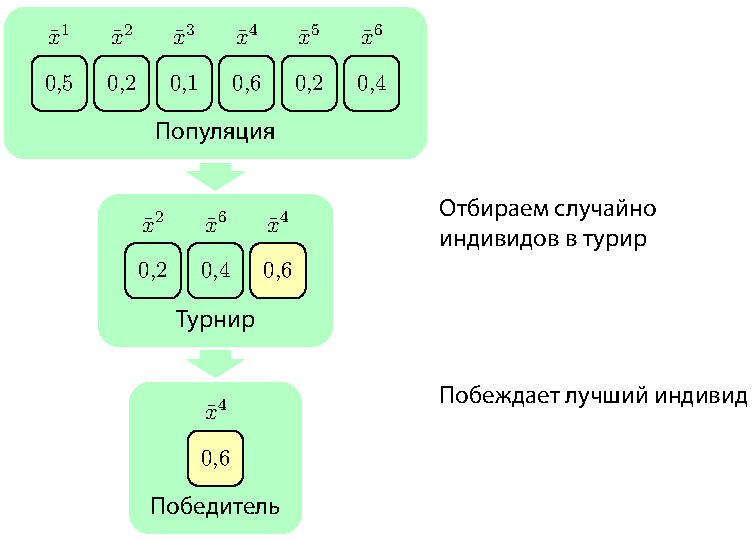
\includegraphics [scale=0.8] {MHL_TournamentSelection_Sheme}
  \caption{Механизм работы турнирной селекции} 
  \label{img:MHL_TournamentSelection_Sheme}  
\end{figure}




\begin{lstlisting}[label=code_use_MHL_TournamentSelection,caption=Пример использования]
        int i;
        int VMHL_N=7;//Размер массива
        double *Fitness;
        Fitness=new double[VMHL_N];
        for (i=0;i<VMHL_N;i++)
         Fitness[i]=MHL_RandomNumber();

        int SizeTournament=3;// Размер турнира

        //Вызов функции
        int Number=MHL_TournamentSelection(Fitness,SizeTournament,VMHL_N);

        //Используем полученный результат

        MHL_ShowVector (Fitness,VMHL_N,"Массив пригодностей", "Fitness");
        //Массив пригодностей:
        //Fitness =
        //0.858643
        //0.460541
        //0.469696
        //0.454315
        //0.594543
        //0.000457764
        //0.476135


        MHL_ShowNumber (SizeTournament,"Размер турнираа", "SizeTournament");
        // Размер турнираа:
        //SizeTournament=3

        MHL_ShowNumber (Number,"Номер выбранного индивида", "Number");
        //Номер выбранного индивида:
        //Number=6

        delete [] Fitness;

        //Для переопределенной функции
        VMHL_N=7;//Размер массива
        Fitness=new double[VMHL_N];
        for (i=0;i<VMHL_N;i++)
         Fitness[i]=MHL_RandomNumber();

        int *Taken;//Информация о том, в турнире или нет индивид (Служебный массив)
        Taken=new int[VMHL_N];

        SizeTournament=3;// Размер турнира

        //Вызов функции
        Number=MHL_TournamentSelection(Fitness,SizeTournament,Taken,VMHL_N);

        //Используем полученный результат

        MHL_ShowVector (Fitness,VMHL_N,"Массив пригодностей", "Fitness");
        //Массив пригодностей:
        //Fitness =
        //0.598633
        //0.396423
        //0.756683
        //0.123505
        //0.0546875
        //0.542511
        //0.605499

        MHL_ShowNumber (SizeTournament,"Размер турнира", "SizeTournament");
        //Размер турнира:
        //SizeTournament=3

        MHL_ShowNumber (Number,"Номер выбранного индивида", "Number");
        //Номер выбранного индивида:
        //Number=2

        delete [] Fitness;
        delete [] Taken;
\end{lstlisting}

\subsubsection{MHL\_TournamentSelectionWithReturn}\label{MHL_TournamentSelectionWithReturn}

Турнирная селекция с возвращением. Оператор генетического алгоритма. Работает с массивом пригодностей индивидов.


\begin{lstlisting}[label=code_syntax_MHL_TournamentSelectionWithReturn,caption=Синтаксис]
int MHL_TournamentSelectionWithReturn(double *Fitness, int SizeTournament, int VMHL_N);
\end{lstlisting}

\textbf{Входные параметры:}
 
Fitness --- массив пригодностей индивидов;
 
VMHL\_N --- размер массива VectorProbability;
 
SizeTournament --- размер турнира.

\textbf{Возвращаемое значение:} 

 Номер выбранного индивида популяции.

\textbf{Примечание:}

 Не является стандартной реализацией турнирной селекции, так как в классичсекой турнирной селекции в один туринир один и тот же индивид может попасть только один раз.




\begin{lstlisting}[label=code_use_MHL_TournamentSelectionWithReturn,caption=Пример использования]
        int i;
        int VMHL_N=7;//Размер массива
        double *Fitness;
        Fitness=new double[VMHL_N];
        for (i=0;i<VMHL_N;i++)
         Fitness[i]=MHL_RandomNumber();

        int SizeTournament=3;// Размер турнира

        //Вызов функции
        int Number=MHL_TournamentSelectionWithReturn(Fitness,SizeTournament,VMHL_N);

        //Используем полученный результат

        MHL_ShowVector (Fitness,VMHL_N,"Массив пригодностей", "Fitness");
        //Массив пригодностей:
        //Fitness =	
        //0.883148
        //0.370209
        //0.0719604
        //0.311371
        //0.558594
        //0.42215
        //0.011322

        MHL_ShowNumber (Number,"Номер выбранного индивида", "Number");
        //Номер выбранного индивида:
        //Number=4

        delete [] Fitness;
\end{lstlisting}

\subsubsection{TMHL\_MutationBinaryMatrix}\label{TMHL_MutationBinaryMatrix}

Мутация для бинарной матрицы. Оператор генетического алгоритма.


\begin{lstlisting}[label=code_syntax_TMHL_MutationBinaryMatrix,caption=Синтаксис]
template <class T> void TMHL_MutationBinaryMatrix(T **VMHL_ResultMatrix, double ProbabilityOfMutation, int VMHL_N,int VMHL_M);
\end{lstlisting}

\textbf{Входные параметры:}
 
VMHL\_ResultMatrix --- указатель на преобразуемый массив;
 
ProbabilityOfMutation --- вероятность мутации;
 
VMHL\_N --- размер массива VMHL\_ResultMatrix (число строк);
 
VMHL\_M --- размер массива VMHL\_ResultMatrix (число столбцов).

\textbf{Возвращаемое значение:} 

Отсутствует.

\textbf{Принцип работы:}
(на примере одной строки матрицы)

\begin{figure} [h]
  \center
  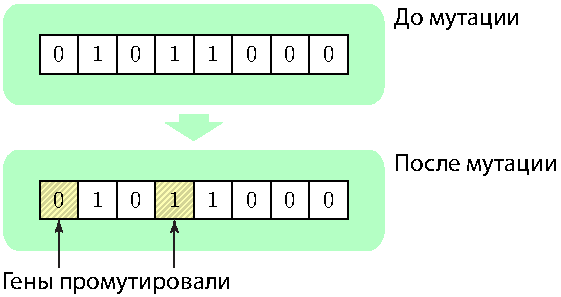
\includegraphics [scale=0.8] {TMHL_MutationBinaryMatrix_Sheme}
  \caption{Механизм работы мутации} 
  \label{img:TMHL_MutationBinaryMatrix_Sheme}  
\end{figure}



\begin{lstlisting}[label=code_use_TMHL_MutationBinaryMatrix,caption=Пример использования]
        int i;
        int VMHL_N=10;//Размер массива (число строк)
        int VMHL_M=3;//Размер массива (число столбцов)
        int **a;
        a=new int*[VMHL_N];
        for (i=0;i<VMHL_N;i++) a[i]=new int[VMHL_M];
        TMHL_RandomBinaryMatrix(a,VMHL_N,VMHL_M);//Случайная бинарная матрица
        MHL_ShowMatrix (a,VMHL_N,VMHL_M,"Случайная бинарная матрица", "a");
        // Случайная бинарная матрица:
        //a =	
        //1	0	1
        //0	0	0
        //0	1	1
        //1	0	1
        //1	0	1
        //1	0	1
        //0	0	1
        //1	1	0
        //1	0	1
        //1	1	0

        double ProbabilityOfMutation=0.1;//Вероятность мутации

        //Вызов функции
        TMHL_MutationBinaryMatrix(a,ProbabilityOfMutation,VMHL_N,VMHL_M);

        //Используем полученный результат
        MHL_ShowMatrix (a,VMHL_N,VMHL_M,"Мутированная бинарная матрица", "a");
        //Мутированная бинарная матрица:
        //a =	
        //1	1	1
        //1	0	0
        //0	1	1
        //1	0	1
        //1	0	1
        //1	0	1
        //0	0	1
        //1	1	0
        //1	0	1
        //1	1	1

        for (i=0;i<VMHL_N;i++) delete [] a[i];
        delete [] a;
\end{lstlisting}

\subsubsection{TMHL\_SinglepointCrossover}\label{TMHL_SinglepointCrossover}

Одноточечное скрещивание. Оператор генетического алгоритма.


\begin{lstlisting}[label=code_syntax_TMHL_SinglepointCrossover,caption=Синтаксис]
template <class T> void TMHL_SinglepointCrossover(T *Parent1, T *Parent2, T *VMHL_ResultVector, int VMHL_N);
\end{lstlisting}

\textbf{Входные параметры:}
 
Parent1 --- первый родитель;
 
Parent2 --- второй родитель;
 
VMHL\_ResultVector --- потомок;
 
VMHL\_N --- размер векторов Parent1, Parent2 и VMHL\_ResultVector.

\textbf{Возвращаемое значение:}

 Отсутствует.
 
\textbf{ Примечание:}

 Потомок выбирается случайно.
 
 \textbf{Формула:}
\begin{align}
&Crossover \left( \overline{Parent}^1, \overline{Parent}^2, DataOfCros\right)=Random \left(\left\lbrace \overline{Offspring}^1; \overline{Offspring}^2\right\rbrace  \right), \nonumber\\
&R=Random\left( \left\lbrace 2; 3; \ldots; n\right\rbrace \right); \nonumber \\
& \overline{Offspring}^1_i=\overline{Parent}^1_i, i=\overline{1,R-1};\nonumber\\
&  \overline{Offspring}^1_i=\overline{Parent}^2_i, i=\overline{R,n};\nonumber\\
&\overline{Offspring}^2_i=\overline{Parent}^2_i, i=\overline{1,R-1};\nonumber\\
& \overline{Offspring}^2_i=\overline{Parent}^1_i, i=\overline{R,n};\nonumber\\
&\overline{Offspring}^1\in X, \overline{Offspring}^2\in X.\nonumber
\end{align}

$ DataOfCros $ не содержит каких-либо параметров относительно данного типа скрещивания.

\textbf{Пример.} Для всех видов скрещивания будем использовать двух родителей: $\overline{Parent}^1\hm={\left( 0; 1; 0; 1; 1; 1; 0; 0\right)}^\mathrm{T}  $ и $\overline{Parent}^2={\left( 1; 1; 0; 0; 1; 0; 1\right)}^\mathrm{T}  $. Одноточечное скрещивание показано на рисунке:

\begin{figure} [h] 
  \center
  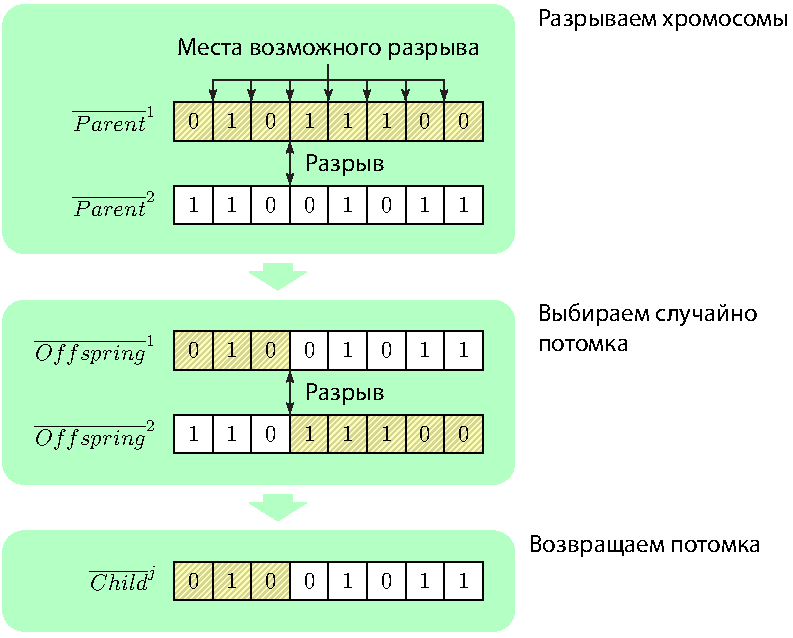
\includegraphics [scale=0.8] {TMHL_SinglepointCrossover_Sheme}
  \caption{Механизм работы одноточечного скрещивания} 
  \label{img:TMHL_SinglepointCrossover_Sheme}  
\end{figure}


\begin{lstlisting}[label=code_use_TMHL_SinglepointCrossover,caption=Пример использования]
        int VMHL_N=10; //Размер массива (число строк)
        int *Parent1;
        Parent1=new int[VMHL_N];
        int *Parent2;
        Parent2=new int[VMHL_N];
        int *Child;
        Child=new int[VMHL_N];
        TMHL_RandomBinaryVector(Parent1,VMHL_N);
        TMHL_RandomBinaryVector(Parent2,VMHL_N);

        //Получим потомка Child
        TMHL_SinglepointCrossover(Parent1,Parent2,Child,VMHL_N);

        //Используем полученный результат
        MHL_ShowVectorT (Parent1,VMHL_N,"Первый родитель", "Parent1");
        //Первый родитель:
        //Parent1 =	
        //0	1	1	0	0	1	0	1	1	1
        
        MHL_ShowVectorT (Parent2,VMHL_N,"Второй родитель", "Parent2");
        //Второй родитель:
        //Parent2 =	
        //0	0	0	1	0	1	0	0	0	0
        
        MHL_ShowVectorT (Child,VMHL_N,"Полученный потомок", "Child");
        //Полученный потомок:
        //Child =	
        //0	1	1	0	0	1	0	1	1	1
        
        delete [] Parent2;
        delete [] Parent1;
        delete [] Child;
\end{lstlisting}

\subsubsection{TMHL\_TwopointCrossover}\label{TMHL_TwopointCrossover}

Двуточечное скрещивание. Оператор генетического алгоритма.


\begin{lstlisting}[label=code_syntax_TMHL_TwopointCrossover,caption=Синтаксис]
template <class T> void TMHL_TwopointCrossover(T *Parent1, T *Parent2, T *VMHL_ResultVector, int VMHL_N);
\end{lstlisting}

\textbf{Входные параметры:}
 
 Parent1 --- первый родитель;
 
 Parent2 --- второй родитель;
 
 VMHL\_ResultVector --- потомок;
 
 VMHL\_N --- размер векторов Parent1, Parent2 и VMHL\_ResultVector.

\textbf{Возвращаемое значение:}

 Отсутствует.
 
\textbf{ Примечание:}

 Потомок выбирается случайно.
 
\begin{align}
&Crossover \left( \overline{Parent}^1, \overline{Parent}^2, DataOfCros\right)=Random \left(\left\lbrace \overline{Offspring}^1; \overline{Offspring}^2\right\rbrace  \right),\nonumber \\
&r_1=Random\left( \left\lbrace 2; 3; \ldots; n\right\rbrace \right); \nonumber \\
&r_2=Random\left( \left\lbrace 2; 3; \ldots; n\right\rbrace \right); \nonumber \\
&R_1=\min \left( r_1, r_2\right) ; \nonumber \\
&R_2=\max \left( r_1, r_2\right) ; \nonumber \\
& \overline{Offspring}^1_i=\overline{Parent}^1_i, i=\overline{1,R_1-1};\nonumber\\
& \overline{Offspring}^1_i=\overline{Parent}^2_i, i=\overline{R_1,R_2-1};\nonumber\\
&  \overline{Offspring}^1_i=\overline{Parent}^1_i, i=\overline{R_2,n};\nonumber\\
& \overline{Offspring}^2_i=\overline{Parent}^2_i, i=\overline{1,R_1-1};\nonumber\\
& \overline{Offspring}^2_i=\overline{Parent}^1_i, i=\overline{R_1,R_2-1};\nonumber\\
&  \overline{Offspring}^2_i=\overline{Parent}^2_i, i=\overline{R_2,n};\nonumber\\
&\overline{Offspring}^1\in X, \overline{Offspring}^2\in X.
\end{align}

$ DataOfCros $ не содержит каких-либо параметров относительно данного типа скрещивания.

\textbf{Пример.} Двухточечное скрещивание показано на рисунке:

\begin{figure} [h]
  \center
  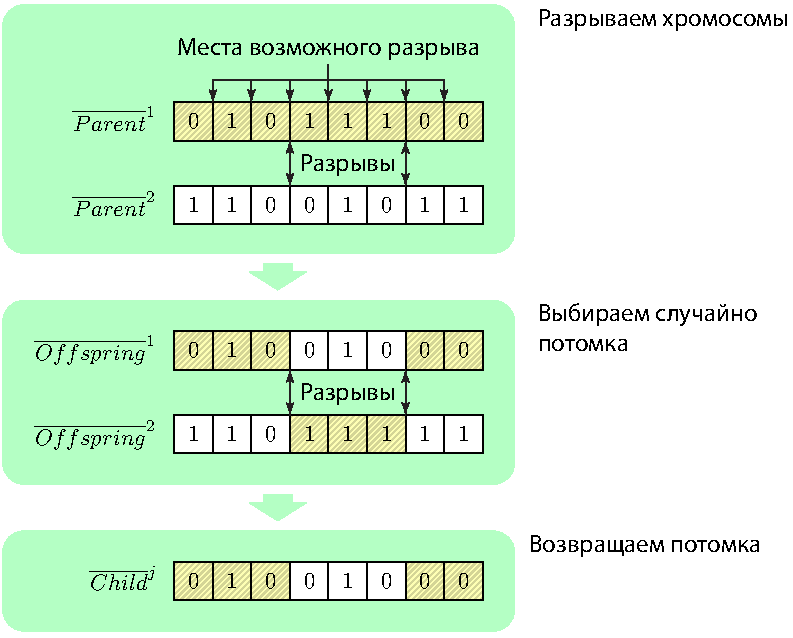
\includegraphics [scale=0.8] {TMHL_TwopointCrossover_Sheme}
  \caption{Механизм работы двухточечного скрещивания} 
  \label{img:TMHL_TwopointCrossover_Sheme}  
\end{figure}


\begin{lstlisting}[label=code_use_TMHL_TwopointCrossover,caption=Пример использования]
        int VMHL_N=10; //Размер массива (число строк)
        int *Parent1;
        Parent1=new int[VMHL_N];
        int *Parent2;
        Parent2=new int[VMHL_N];
        int *Child;
        Child=new int[VMHL_N];
        TMHL_RandomBinaryVector(Parent1,VMHL_N);
        TMHL_RandomBinaryVector(Parent2,VMHL_N);

        //Получим потомка Child
        TMHL_TwopointCrossover(Parent1,Parent2,Child,VMHL_N);

        //Используем полученный результат
        MHL_ShowVectorT (Parent1,VMHL_N,"Первый родитель", "Parent1");
        //Первый родитель:
        //Parent1 =
        //1	1	0	0	1	1	0	0	0	0

        MHL_ShowVectorT (Parent2,VMHL_N,"Второй родитель", "Parent2");
        //Второй родитель:
        //Parent2 =
        //0	1	1	0	0	1	0	0	1	0

        MHL_ShowVectorT (Child,VMHL_N,"Полученный потомок", "Child");
        //Полученный потомок:
        //Child =
        //0	1	1	0	0	1	0	0	1	0

        delete [] Parent2;
        delete [] Parent1;
        delete [] Child;
\end{lstlisting}

\subsubsection{TMHL\_UniformCrossover}\label{TMHL_UniformCrossover}

Равномерное скрещивание. Оператор генетического алгоритма.


\begin{lstlisting}[label=code_syntax_TMHL_UniformCrossover,caption=Синтаксис]
template <class T> void TMHL_UniformCrossover(T *Parent1, T *Parent2, T *VMHL_ResultVector, int VMHL_N);
\end{lstlisting}

\textbf{Входные параметры:}
 
 Parent1 --- первый родитель;
 
 Parent2 --- второй родитель;
 
 VMHL\_ResultVector --- потомок;
 
 VMHL\_N --- размер векторов Parent1, Parent2 и VMHL\_ResultVector.

\textbf{Возвращаемое значение:}

 Отсутствует.
 
\begin{align*}
&Crossover \left( \overline{Parent}^1, \overline{Parent}^2, DataOfCros\right) = \overline{Offspring};\\
& \overline{Offspring}_i=Random\left( \left\lbrace \overline{Parent}^1_i;\overline{Parent}^2_i\right\rbrace \right), i=\overline{1,n} ;\nonumber\\
&\overline{Offspring}\in X.\nonumber
\end{align*}

$ DataOfCros $ не содержит каких-либо параметров относительно данного типа скрещивания.

\textbf{Пример.} Двухточечное скрещивание показано на рисунке:

\begin{figure} [h]
  \center
  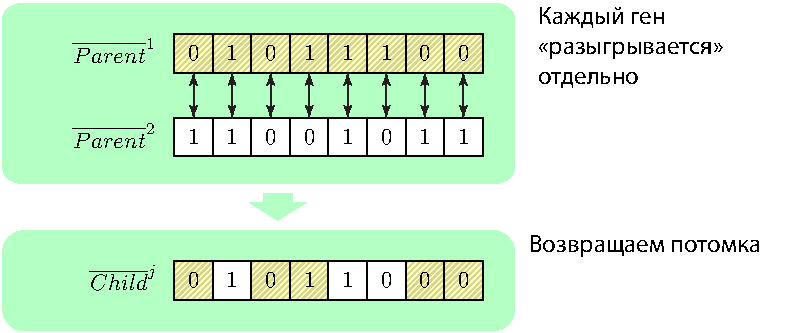
\includegraphics [scale=0.8] {TMHL_UniformCrossover_Sheme}
  \caption{Механизм работы равномерного скрещивания} 
  \label{img:TMHL_UniformCrossover_Sheme}  
\end{figure}


\begin{lstlisting}[label=code_use_TMHL_UniformCrossover,caption=Пример использования]
        int VMHL_N=10; //Размер массива (число строк)
        int *Parent1;
        Parent1=new int[VMHL_N];
        int *Parent2;
        Parent2=new int[VMHL_N];
        int *Child;
        Child=new int[VMHL_N];
        TMHL_RandomBinaryVector(Parent1,VMHL_N);
        TMHL_RandomBinaryVector(Parent2,VMHL_N);

        //Получим потомка Child
        TMHL_UniformCrossover(Parent1,Parent2,Child,VMHL_N);

        //Используем полученный результат
        MHL_ShowVectorT (Parent1,VMHL_N,"Первый родитель", "Parent1");
        //Первый родитель:
        //Parent1 =	
        //1	1	0	1	1	1	1	1	1	0
        
        MHL_ShowVectorT (Parent2,VMHL_N,"Второй родитель", "Parent2");
        //Второй родитель:
        //Parent2 =	
        //0	0	0	0	1	0	1	1	0	0
        
        MHL_ShowVectorT (Child,VMHL_N,"Полученный потомок", "Child");
        //Полученный потомок:
        //Child =	
        //1	1	0	0	1	0	1	1	1	0
        
        delete [] Parent2;
        delete [] Parent1;
        delete [] Child;
\end{lstlisting}

\subsection{Геометрия}

\subsubsection{TMHL\_BoolCrossingTwoSegment}\label{TMHL_BoolCrossingTwoSegment}

Функция определяет наличие пересечения двух отрезков. Координаты отрезков могут быть перепутаны по порядку в каждом отрезке.


\begin{lstlisting}[label=code_syntax_TMHL_BoolCrossingTwoSegment,caption=Синтаксис]
template <class T> int TMHL_BoolCrossingTwoSegment(T b1,T c1,T b2,T c2);
\end{lstlisting}

\textbf{Входные параметры:}  
 
b1 --- левый конец первого отрезка;
 
c1 --- правый конец первого отрезка;
 
b2 --- левый конец второго отрезка;
 
с2 --- правый конец второго отрезка.

\textbf{Возвращаемое значение:}
 
1 --- отрезки пересекаются;
 
0 --- отрезки не пересекаются.


\begin{lstlisting}[label=code_use_TMHL_BoolCrossingTwoSegment,caption=Пример использования]
        double b1,c1,b2,c2;
        int Result;
        //Зададим случайные координаты отрезков
        b1=MHL_RandomUniform(-3,5);
        c1=MHL_RandomUniform(-3,5);
        b2=MHL_RandomUniform(-3,5);
        c2=MHL_RandomUniform(-3,5);

        //Вызов функции
        Result=TMHL_BoolCrossingTwoSegment(b1,c1,b2,c2);

        //Используем полученный результат
        MHL_ShowNumber (b1,"Левый конец первого отрезка", "b1");
        //Левый конец первого отрезка:
        //b1=0.773193
        MHL_ShowNumber (c1,"Правый конец первого отрезка", "c1");
        //Правый конец первого отрезка:
        //c1=3.22803
        MHL_ShowNumber (b2,"Левый конец второго отрезка", "b2");
        //Левый конец второго отрезка:
        //b2=4.99121
        MHL_ShowNumber (c2,"Правый конец второго отрезка", "c2");
        //Правый конец второго отрезка:
        //c2=1.43921
        MHL_ShowNumber (Result,"Пересекаются ли отрезки", "Result");
        //Пересекаются ли отрезки:
        //Result=1
\end{lstlisting}

\subsection{Гиперболические функции}

\subsubsection{MHL\_Cosech}\label{MHL_Cosech}

Функция возвращает гиперболический косеканс.


\begin{lstlisting}[label=code_syntax_MHL_Cosech,caption=Синтаксис]
double MHL_Cosech(double x);
\end{lstlisting}

\textbf{Входные параметры:}

 x --- входная переменная.

\textbf{Возвращаемое значение:}

Гиперболический косеканс.


\begin{lstlisting}[label=code_use_MHL_Cosech,caption=Пример использования]
        double x=MHL_RandomUniform(0,10);

        //Вызов функции
        double Result=MHL_Cosech(x);

        //Используем полученный результат
        MHL_ShowNumber(Result,"Гиперболический косеканс от x="+MHL_NumberToText(x),"равен");
        //Гиперболический косеканс от x=0.571289:
        //равен=1.65872
\end{lstlisting}

\subsubsection{MHL\_Cosh}\label{MHL_Cosh}

Функция возвращает гиперболический косинус.


\begin{lstlisting}[label=code_syntax_MHL_Cosh,caption=Синтаксис]
double MHL_Cosh(double x);
\end{lstlisting}

\textbf{Входные параметры:}

 x --- входная переменная.

\textbf{Возвращаемое значение:}

Гиперболический косинус.


\begin{lstlisting}[label=code_use_MHL_Cosh,caption=Пример использования]
        double x=MHL_RandomUniform(0,10);

        //Вызов функции
        double Result=MHL_Cosh(x);

        //Используем полученный результат
        MHL_ShowNumber(Result,"Гиперболический косинус от x="+MHL_NumberToText(x),"равен");
        //Гиперболический косинус от x=4.04968:
        //равен=28.6983
\end{lstlisting}

\subsubsection{MHL\_Cotanh}\label{MHL_Cotanh}

Функция возвращает гиперболический котангенс.


\begin{lstlisting}[label=code_syntax_MHL_Cotanh,caption=Синтаксис]
double MHL_Cotanh(double x);
\end{lstlisting}

\textbf{Входные параметры:}

 x --- входная переменная.

\textbf{Возвращаемое значение:}

Гиперболический котангенс.


\begin{lstlisting}[label=code_use_MHL_Cotanh,caption=Пример использования]
        double x=MHL_RandomUniform(0,10);

        //Вызов функции
        double Result=MHL_Cotanh(x);

        //Используем полученный результат
        MHL_ShowNumber(Result,"Гиперболический котангенс от x="+MHL_NumberToText(x),"равен");
        //Гиперболический котангенс от x=1.92505:
        //равен=1.04348
\end{lstlisting}

\subsubsection{MHL\_Sech}\label{MHL_Sech}

Функция возвращает гиперболический секанс.


\begin{lstlisting}[label=code_syntax_MHL_Sech,caption=Синтаксис]
double MHL_Sech(double x);
\end{lstlisting}

\textbf{Входные параметры:}

 x --- входная переменная.

\textbf{Возвращаемое значение:}

Гиперболический секанс.


\begin{lstlisting}[label=code_use_MHL_Sech,caption=Пример использования]
        double x=MHL_RandomUniform(0,10);

        //Вызов функции
        double Result=MHL_Sech(x);

        //Используем полученный результат
        MHL_ShowNumber(Result,"Гиперболический секанс от x="+MHL_NumberToText(x),"равен");
        //Гиперболический секанс от x=0.679932:
        //равен=0.806323
\end{lstlisting}

\subsubsection{MHL\_Sinh}\label{MHL_Sinh}

Функция возвращает гиперболический синус.


\begin{lstlisting}[label=code_syntax_MHL_Sinh,caption=Синтаксис]
double MHL_Sinh(double x);
\end{lstlisting}

\textbf{Входные параметры:}

 x --- входная переменная.

\textbf{Возвращаемое значение:}

Гиперболический синус.


\begin{lstlisting}[label=code_use_MHL_Sinh,caption=Пример использования]
        double x=MHL_RandomUniform(0,10);

        //Вызов функции
        double Result=MHL_Sinh(x);

        //Используем полученный результат
        MHL_ShowNumber(Result,"Гиперболический синус от x="+MHL_NumberToText(x),"равен");
        //Гиперболический синус от x=0.166321:
        //равен=0.167089
\end{lstlisting}

\subsubsection{MHL\_Tanh}\label{MHL_Tanh}

Функция возвращает гиперболический тангенс.


\begin{lstlisting}[label=code_syntax_MHL_Tanh,caption=Синтаксис]
double MHL_Tanh(double x);
\end{lstlisting}

\textbf{Входные параметры:}

 x --- входная переменная.

\textbf{Возвращаемое значение:}

Гиперболический тангенс.


\begin{lstlisting}[label=code_use_MHL_Tanh,caption=Пример использования]
        double x=MHL_RandomUniform(0,10);

        //Вызов функции
        double Result=MHL_Tanh(x);

        //Используем полученный результат
        MHL_ShowNumber(Result,"Гиперболический тангенс от x="+MHL_NumberToText(x),"равен");
        //Гиперболический тангенс от x=4.27643:
        //равен=0.999614
\end{lstlisting}

\subsection{Дифференцирование}

\subsubsection{MHL\_CenterDerivative}\label{MHL_CenterDerivative}

Численное значение производной в точке (центральной разностной производной с шагом 2h).


\begin{lstlisting}[label=code_syntax_MHL_CenterDerivative,caption=Синтаксис]
double MHL_CenterDerivative(double x, double h, double (*Function)(double));
\end{lstlisting}

\textbf{Входные параметры:}
 x --- точка, в которой считается производная;
 
 h --- малое приращение x;
 
 Function --- функция, производная которой ищется.

\textbf{Возвращаемое значение:}
 
 Значение производной в точке.
 
 \textbf{Примечание:}
 
 При $h\leq0$ возвращается $0$.

\textbf{Формула:}
\begin{eqnarray*}
f'\left( x\right) \approx \dfrac{f\left( x+h\right)-f\left( x-h\right) }{2\cdot h}
\end{eqnarray*}

Будем использовать в примере использования дополнительную функцию.

\begin{lstlisting}[caption=Дополнительная функция]
double Func3(double x)
{
return x*x;
}
//---------------------------------------------------------------------------
\end{lstlisting}


\begin{lstlisting}[label=code_use_MHL_CenterDerivative,caption=Пример использования]
        double x;
        double h;
        double dfdx;
        //Зададим случайные координаты отрезков
        x=MHL_RandomUniform(-3,5);
        h=0.01;//малое приращение x

        //Вызов функции
        dfdx=MHL_CenterDerivative(x,h,Func3);

        //Используем полученный результат
        MHL_ShowNumber (x,"Точка, в которой считается производная", "x");
        //Точка, в которой считается производная:
        //x=0.843262
        MHL_ShowNumber (h,"Малое приращение x", "h");
        // Малое приращение x:
        //h=0.01
        MHL_ShowNumber (dfdx,"Значение производной в точке", "dfdx");
        // Значение производной в точке:
        //dfdx=1.68652
\end{lstlisting}

\subsubsection{MHL\_LeftDerivative}\label{MHL_LeftDerivative}

Численное значение производной в точке (разностная производная влево).


\begin{lstlisting}[label=code_syntax_MHL_LeftDerivative,caption=Синтаксис]
double MHL_LeftDerivative(double x, double h, double (*Function)(double));
\end{lstlisting}

\textbf{Входные параметры:}
 x --- точка, в которой считается производная;
 
 h --- малое приращение x;
 
 Function --- функция, производная которой ищется.

\textbf{Возвращаемое значение:}
 
 Значение производной в точке.
 
 \textbf{Примечание:}
 
 При $h\leq0$ возвращается $0$.

\textbf{Формула:}
\begin{eqnarray*}
f'\left( x\right) \approx \dfrac{f\left( x\right)-f\left( x-h\right) }{h}
\end{eqnarray*}

Будем использовать в примере использования дополнительную функцию.

\begin{lstlisting}[caption=Дополнительная функция]
double Func3(double x)
{
return x*x;
}
//---------------------------------------------------------------------------
\end{lstlisting}


\begin{lstlisting}[label=code_use_MHL_LeftDerivative,caption=Пример использования]
        double x;
        double h;
        double dfdx;
        //Зададим случайные координаты отрезков
        x=MHL_RandomUniform(-3,5);
        h=0.01;//малое приращение x

        //Вызов функции
        dfdx=MHL_LeftDerivative(x,h,Func3);

        //Используем полученный результат
        MHL_ShowNumber (x,"Точка, в которой считается производная", "x");
        // Точка, в которой считается производная:
        //x=1.87964
        MHL_ShowNumber (h,"Малое приращение x", "h");
        // Малое приращение x:
        //h=0.01
        MHL_ShowNumber (dfdx,"Значение производной в точке", "dfdx");
        // Значение производной в точке:
        //dfdx=3.74928
\end{lstlisting}

\subsubsection{MHL\_RightDerivative}\label{MHL_RightDerivative}

Численное значение производной в точке (разностная производная вправо).


\begin{lstlisting}[label=code_syntax_MHL_RightDerivative,caption=Синтаксис]
double MHL_RightDerivative(double x, double h, double (*Function)(double));
\end{lstlisting}

\textbf{Входные параметры:}
 x --- точка, в которой считается производная;
 
 h --- малое приращение x;
 
 Function --- функция, производная которой ищется.

\textbf{Возвращаемое значение:}
 
 Значение производной в точке.
 
 \textbf{Примечание:}
 
 При $h\leq0$ возвращается $0$.

\textbf{Формула:}
\begin{eqnarray*}
f'\left( x\right) \approx \dfrac{f\left( x+h\right)-f\left( x\right) }{h}
\end{eqnarray*}

Будем использовать в примере использования дополнительную функцию.

\begin{lstlisting}[caption=Дополнительная функция]
double Func3(double x)
{
return x*x;
}
//---------------------------------------------------------------------------
\end{lstlisting}


\begin{lstlisting}[label=code_use_MHL_RightDerivative,caption=Пример использования]
        double x;
        double h;
        double dfdx;
        //Зададим случайные координаты отрезков
        x=MHL_RandomUniform(-3,5);
        h=0.01;//малое приращение x

        //Вызов функции
        dfdx=MHL_RightDerivative(x,h,Func3);

        //Используем полученный результат
        MHL_ShowNumber (x,"Точка, в которой считается производная", "x");
        // Точка, в которой считается производная:
        //x=-1.69409
        MHL_ShowNumber (h,"Малое приращение x", "h");
        // Малое приращение x:
        //h=0.01
        MHL_ShowNumber (dfdx,"Значение производной в точке", "dfdx");
        // Значение производной в точке:
        //dfdx=-3.37818
\end{lstlisting}

\subsection{Для тестовых функций}

\subsubsection{MHL\_DefineTestFunction}\label{MHL_DefineTestFunction}

Служебная функция определяет тестовую функцию для других функций по работе с тестовыми функциями.


\begin{lstlisting}[label=code_syntax_MHL_DefineTestFunction,caption=Синтаксис]
void MHL_DefineTestFunction(TypeOfTestFunction Type);
\end{lstlisting}

\textbf{Входные параметры:}
  
Type --- обозначение тестовой функции, которую вызываем.
Смотреть виды в переменных перечисляемого типа в начале MathHarrixLibrary.h файла: TestFunction\_Ackley, TestFunction\_ParaboloidOfRevolution, TestFunction\_Rastrigin и др. Они совпадают с названиями одноименных тестовых функций, но без приставки \textbf{MHL\_}.

\textbf{Возвращаемое значение:}
 
Отсутствует.


\begin{lstlisting}[label=code_use_MHL_DefineTestFunction,caption=Пример использования]
    //Вызов функции
    MHL_DefineTestFunction(TestFunction_SumVector);

    //Использование результата
    int N=5;
    int *x=new int[N];
    TMHL_RandomBinaryVector(x,N);
    double f=MHL_TestFunction_Binary(x,N);

    MHL_ShowVectorT(x,N,"Решение","x");
    //Решение:
    //x =	
    //1	1	1	1	0

    MHL_ShowNumber(f,"Значение целевой функции","f");
    //Значение целевой функции:
    //f=4
\end{lstlisting}

\subsubsection{MHL\_ErrorExOfTestFunction\_Binary}\label{MHL_ErrorExOfTestFunction_Binary}

Функция определяет значение ошибки по входным параметрам найденного решения в задаче оптимизации для тестовой функции. Включает в себя все тестовые функции. Есть функция-переопределение, где пользователь может сам указать тип тестовой функции.


\begin{lstlisting}[label=code_syntax_MHL_ErrorExOfTestFunction_Binary,caption=Синтаксис]
double MHL_ErrorExOfTestFunction_Binary(int *x, int VMHL_N);
double MHL_ErrorExOfTestFunction_Binary(int *x, int VMHL_N, TypeOfTestFunction Type);
\end{lstlisting}

\textbf{Входные параметры:}

x --- указатель на исходный массив (найденное решение алгоритмом);

VMHL\_N --- размер массива x.

В переопределяемой функции также есть параметр:
  
Type --- обозначение тестовой функции, которую вызываем.
Смотреть виды в переменных перечисляемого типа в начале MathHarrixLibrary.h файла: TestFunction\_Ackley, TestFunction\_ParaboloidOfRevolution, TestFunction\_Rastrigin и др. Они совпадают с названиями одноименных тестовых функций, но без приставки \textbf{MHL\_}.

\textbf{Возвращаемое значение:}
 
Значение ошибки по входным параметрам Ex.

Итак, для обычного использования (без параметра Type) нужно вызвать функцию MHL\_DefineTestFunction. Иначе использовать переопределенную функцию и самому указать тип тестовой функции.

Конкретную формулу, которые используются для нахождения для каждой тестовой функции, смотрите в функциях этих тестовых функций. Обратите внимание, что данная функция находит ошибку только для одного решения, тогда как по формулам нужно множество решений.


\begin{lstlisting}[label=code_use_MHL_ErrorExOfTestFunction_Binary,caption=Пример использования]
        MHL_DefineTestFunction(TestFunction_SumVector);

        int N=5;
        int *x=new int[N];
        TMHL_RandomBinaryVector(x,N);

        //Вызов функции
        double Ex=MHL_ErrorExOfTestFunction_Binary(x,N);

        //Использование результата
        MHL_ShowVectorT(x,N,"Решение","x");
        //Решение:
        //x =	
        //1	0	1	1	1

        MHL_ShowNumber(Ex,"Значение ошибки по входным параметрам","E<sub>x</sub>");
        //Значение ошибки по входным параметрам:
        //Ex=1
\end{lstlisting}

\subsubsection{MHL\_ErrorEyOfTestFunction\_Binary}\label{MHL_ErrorEyOfTestFunction_Binary}

Функция определяет значение ошибки по значениям целевой функции найденного решения в задаче оптимизации для тестовой функции. Включает в себя все тестовые функции. Есть функция-переопределение, где пользователь может сам указать тип тестовой функции.


\begin{lstlisting}[label=code_syntax_MHL_ErrorEyOfTestFunction_Binary,caption=Синтаксис]
double MHL_ErrorEyOfTestFunction_Binary(double FitnessOfx, int VMHL_N);
double MHL_ErrorEyOfTestFunction_Binary(double FitnessOfx, int VMHL_N, TypeOfTestFunction Type);
\end{lstlisting}

\textbf{Входные параметры:}

FitnessOfx --- значение целевой функции найденного решения алгоритмом оптимизации;

VMHL\_N --- размер массива x.

В переопределяемой функции также есть параметр:
  
Type --- обозначение тестовой функции, которую вызываем.
Смотреть виды в переменных перечисляемого типа в начале MathHarrixLibrary.h файла: TestFunction\_Ackley, TestFunction\_ParaboloidOfRevolution, TestFunction\_Rastrigin и др. Они совпадают с названиями одноименных тестовых функций, но без приставки \textbf{MHL\_}.

\textbf{Возвращаемое значение:}
 
Значение ошибки по значениям целевой функции Ey.

Итак, для обычного использования (без параметра Type) нужно вызвать функцию MHL\_DefineTestFunction. Иначе использовать переопределенную функцию и самому указать тип тестовой функции.

Конкретную формулу, которые используются для нахождения для каждой тестовой функции, смотрите в функциях этих тестовых функций. Обратите внимание, что данная функция находит ошибку только для одного решения, тогда как по формулам нужно множество решений.


\begin{lstlisting}[label=code_use_MHL_ErrorEyOfTestFunction_Binary,caption=Пример использования]
        MHL_DefineTestFunction(TestFunction_SumVector);

        int N=5;
        int *x=new int[N];
        TMHL_RandomBinaryVector(x,N);
        double f=MHL_TestFunction_Binary(x,N);

        //Вызов функции
        double Ey=MHL_ErrorEyOfTestFunction_Binary(f,N);

        //Использование результата
        MHL_ShowVectorT(x,N,"Решение","x");
        //Решение:
        //x =	
        //0	1	1	0	1

        MHL_ShowNumber(Ey,"Значение ошибки по значениям целевой функции","E<sub>y</sub>");
        //Значение ошибки по значениям целевой функции:
        //Ey=2
\end{lstlisting}

\subsubsection{MHL\_ErrorROfTestFunction\_Binary}\label{MHL_ErrorROfTestFunction_Binary}

Функция определяет значение надежности найденного решения в задаче оптимизации для тестовой функции. Включает в себя все тестовые функции. Есть функция-переопределение, где пользователь может сам указать тип тестовой функции.


\begin{lstlisting}[label=code_syntax_MHL_ErrorROfTestFunction_Binary,caption=Синтаксис]
double MHL_ErrorROfTestFunction_Binary(int *x, int VMHL_N);
double MHL_ErrorROfTestFunction_Binary(int *x, int VMHL_N, TypeOfTestFunction Type);
\end{lstlisting}

\textbf{Входные параметры:}

x --- указатель на исходный массив (найденное решение алгоритмом);

VMHL\_N --- размер массива x.

В переопределяемой функции также есть параметр:
  
Type --- обозначение тестовой функции, которую вызываем.
Смотреть виды в переменных перечисляемого типа в начале MathHarrixLibrary.h файла: TestFunction\_Ackley, TestFunction\_ParaboloidOfRevolution, TestFunction\_Rastrigin и др. Они совпадают с названиями одноименных тестовых функций, но без приставки \textbf{MHL\_}.

\textbf{Возвращаемое значение:}
 
Значение надежности R.

Итак, для обычного использования (без параметра Type) нужно вызвать функцию MHL\_DefineTestFunction. Иначе использовать переопределенную функцию и самому указать тип тестовой функции.

Конкретную формулу, которые используются для нахождения для каждой тестовой функции, смотрите в функциях этих тестовых функций. Обратите внимание, что данная функция находит ошибку только для одного решения, тогда как по формулам нужно множество решений.


\begin{lstlisting}[label=code_use_MHL_ErrorROfTestFunction_Binary,caption=Пример использования]
        MHL_DefineTestFunction(TestFunction_SumVector);

        int N=5;
        int *x=new int[N];
        TMHL_RandomBinaryVector(x,N);

        //Вызов функции
        double R=MHL_ErrorROfTestFunction_Binary(x,N);

        //Использование результата
        MHL_ShowVectorT(x,N,"Решение","x");
        //Решение:
        //x =
        //1	1	1	1	1

        MHL_ShowNumber(R,"Значение надежности","R");
        //Значение надежности:
        //R=1
\end{lstlisting}

\subsubsection{MHL\_FitnessOfOptimumOfTestFunction\_Binary}\label{MHL_FitnessOfOptimumOfTestFunction_Binary}

Функция определяет значение целевой функции в оптимуме для тестовой функции. Включает в себя все тестовые функции. Есть функция-переопределение, где пользователь может сам указать тип тестовой функции.


\begin{lstlisting}[label=code_syntax_MHL_FitnessOfOptimumOfTestFunction_Binary,caption=Синтаксис]
double MHL_FitnessOfOptimumOfTestFunction_Binary(int VMHL_N);
double MHL_FitnessOfOptimumOfTestFunction_Binary(int VMHL_N, TypeOfTestFunction Type);
\end{lstlisting}

\textbf{Входные параметры:}

VMHL\_N --- размер массива x.

В переопределяемой функции также есть параметр:
  
Type --- обозначение тестовой функции, которую вызываем.
Смотреть виды в переменных перечисляемого типа в начале MathHarrixLibrary.h файла: TestFunction\_Ackley, TestFunction\_ParaboloidOfRevolution, TestFunction\_Rastrigin и др. Они совпадают с названиями одноименных тестовых функций, но без приставки \textbf{MHL\_}.

\textbf{Возвращаемое значение:}
 
Значение тестовой функции в оптимальной точке.

Итак, для обычного использования (без параметра Type) нужно вызвать функцию MHL\_DefineTestFunction. Иначе использовать переопределенную функцию и самому указать тип тестовой функции.


\begin{lstlisting}[label=code_use_MHL_FitnessOfOptimumOfTestFunction_Binary,caption=Пример использования]
        MHL_DefineTestFunction(TestFunction_SumVector);

        int N=5;

        //Вызов функции
        double f=MHL_FitnessOfOptimumOfTestFunction_Binary(N);

        //Использование результата
        MHL_ShowNumber(f,"Значение целевой функции оптимального решения","f");
        //Значение целевой функции оптимального решения:
        //f=5
\end{lstlisting}

\subsubsection{MHL\_GetCountOfFitness}\label{MHL_GetCountOfFitness}

Функция выдает количество вызовов целевой функции.


\begin{lstlisting}[label=code_syntax_MHL_GetCountOfFitness,caption=Синтаксис]
int MHL_GetCountOfFitness();
\end{lstlisting}

\textbf{Входные параметры:}

Отсутствуют.

\textbf{Возвращаемое значение:}
 
Количество вызовов целевой функции.

Данную функцию надо использовать в связке с функцией MHL\_GetCountOfFitness(). Для чего использовать эти функции? Дело в том, что для сравнения алгоритмов оптимизации очень критично оценивать вызов целевой функции. И часто многие программисты пишут или не очень акккуратно, или логика алгоритма такая, что заявленное число вычислений функций не совпадает с действительным. Поэтому в общие тестовые функции (например, MHL\_TestFunction\_Binary) вшит подсчет числа вызовов целевой функции.

MHL\_SetToZeroCountOfFitness --- эту функцию вызываем перед вызовом какого-то алгоритма оптимизации, а MHL\_GetCountOfFitness --- после его работы.


\begin{lstlisting}[label=code_use_MHL_GetCountOfFitness,caption=Пример использования]
        MHL_DefineTestFunction(TestFunction_SumVector);

        MHL_SetToZeroCountOfFitness();

        int N=5;
        double f=0;
        int *x=new int[N];

        for (int i=0;i<10;i++)
        {
            TMHL_RandomBinaryVector(x,N);
            f+=MHL_TestFunction_Binary(x,N);
        }

        f/=double(10.);

        //Вызов функции
        int M=MHL_GetCountOfFitness();

        //Использование результата
        MHL_ShowNumber(M,"Количество вызовов целевой функции","M");
        //Количество вызовов целевой функции:
        //M=10

        MHL_ShowNumber(f,"Среднее значение целевой функции","f");
        //Среднее значение целевой функции:
        //f=2.6
\end{lstlisting}

\subsubsection{MHL\_OptimumOfTestFunction\_Binary}\label{MHL_OptimumOfTestFunction_Binary}

Функция определяет значение оптимума для тестовой функции. Включает в себя все тестовые функции. Есть функция-переопределение, где пользователь может сам указать тип тестовой функции.


\begin{lstlisting}[label=code_syntax_MHL_OptimumOfTestFunction_Binary,caption=Синтаксис]
double MHL_OptimumOfTestFunction_Binary(int *Optimum, int VMHL_N);
double MHL_OptimumOfTestFunction_Binary(int *Optimum, int VMHL_N, TypeOfTestFunction Type);
\end{lstlisting}

\textbf{Входные параметры:}

Optimum --- указатель на исходный массив, куда будет записываться результат? то есть оптимум тестовой функции (максимум или минимум --- это зависит от типа тестовой функции, что расписывается в самих функциях тестовых функций);

     VMHL\_N --- размер массива x.

В переопределяемой функции также есть параметр:
  
Type --- обозначение тестовой функции, которую вызываем.
Смотреть виды в переменных перечисляемого типа в начале MathHarrixLibrary.h файла: TestFunction\_Ackley, TestFunction\_ParaboloidOfRevolution, TestFunction\_Rastrigin и др. Они совпадают с названиями одноименных тестовых функций, но без приставки \textbf{MHL\_}.

\textbf{Возвращаемое значение:}
 
Значение тестовой функции в оптимальной точке.

Итак, для обычного использования (без параметра Type) нужно вызвать функцию MHL\_DefineTestFunction. Иначе использовать переопределенную функцию и самому указать тип тестовой функции.


\begin{lstlisting}[label=code_use_MHL_OptimumOfTestFunction_Binary,caption=Пример использования]
        MHL_DefineTestFunction(TestFunction_SumVector);

        int N=5;
        int *x=new int[N];

        //Вызов функции
        double f=MHL_OptimumOfTestFunction_Binary(x,N);

        //Использование результата
        MHL_ShowVectorT(x,N,"Оптимальное решение тестовой функции TestFunction_SumVector","x");
        //Оптимальное решение тестовой функции TestFunction_SumVector:
        //x =	
        //1	1	1	1	1

        MHL_ShowNumber(f,"Значение целевой функции оптимального решения","f");
        //Значение целевой функции оптимального решения:
        //f=5
\end{lstlisting}

\subsubsection{MHL\_SetToZeroCountOfFitness}\label{MHL_SetToZeroCountOfFitness}

Функция обнуляет количество вызовов целевой функции. Обязательно вызвать один раз перед вызовом алгоритмов оптимизации при исследовании эффективности    алгоритмов оптимизации, где требуется контроль числа вызовов целевой функции.


\begin{lstlisting}[label=code_syntax_MHL_SetToZeroCountOfFitness,caption=Синтаксис]
void MHL_SetToZeroCountOfFitness();
\end{lstlisting}

\textbf{Входные параметры:}

Отсутствуют.

\textbf{Возвращаемое значение:}
 
Отсутствует.

Данную функцию надо использовать в связке с функцией MHL\_GetCountOfFitness(). Для чего использовать эти функции? Дело в том, что для сравнения алгоритмов оптимизации очень критично оценивать вызов целевой функции. И часто многие программисты пишут или не очень акккуратно, или логика алгоритма такая, что заявленное число вычислений функций не совпадает с действительным. Поэтому в общие тестовые функции (например, MHL\_TestFunction\_Binary) вшит подсчет числа вызовов целевой функции.

MHL\_SetToZeroCountOfFitness --- эту функцию вызываем перед вызовом какого-то алгоритма оптимизации, а MHL\_GetCountOfFitness --- после его работы.


\begin{lstlisting}[label=code_use_MHL_SetToZeroCountOfFitness,caption=Пример использования]
        MHL_DefineTestFunction(TestFunction_SumVector);

        //Вызов функции
        MHL_SetToZeroCountOfFitness();

        //Использование результата
        int N=5;
        double f=0;
        int *x=new int[N];

        for (int i=0;i<10;i++)
        {
            TMHL_RandomBinaryVector(x,N);
            f+=MHL_TestFunction_Binary(x,N);
        }

        f/=double(10.);

        int M=MHL_GetCountOfFitness();
        MHL_ShowNumber(M,"Количество вызовов целевой функции","M");
        //Количество вызовов целевой функции:
        //M=10

        MHL_ShowNumber(f,"Среднее значение целевой функции","f");
        //Среднее значение целевой функции:
        //f=2.6
\end{lstlisting}

\subsubsection{MHL\_TestFunction\_Binary}\label{MHL_TestFunction_Binary}

Общая тестовая функция для задач бинарной оптимизации. Есть функция-переопределение, где пользователь может сам указать тип тестовой функции.


\begin{lstlisting}[label=code_syntax_MHL_TestFunction_Binary,caption=Синтаксис]
double MHL_TestFunction_Binary(int *x, int VMHL_N);
double MHL_TestFunction_Binary(int *x, int VMHL_N, TypeOfTestFunction Type);
\end{lstlisting}

\textbf{Входные параметры:}

x --- указатель на исходный массив;

VMHL\_N --- размер массива x.

В переопределяемой функции также есть параметр:
  
Type --- обозначение тестовой функции, которую вызываем.
Смотреть виды в переменных перечисляемого типа в начале MathHarrixLibrary.h файла: TestFunction\_Ackley, TestFunction\_ParaboloidOfRevolution, TestFunction\_Rastrigin и др. Они совпадают с названиями одноименных тестовых функций, но без приставки \textbf{MHL\_}.

\textbf{Возвращаемое значение:}
 
Значение тестовой функции в точке x.

Итак, для обычного использования (без параметра Type) нужно вызвать функцию MHL\_DefineTestFunction. Иначе использовать переопределенную функцию и самому указать тип тестовой функции.


\begin{lstlisting}[label=code_use_MHL_TestFunction_Binary,caption=Пример использования]
        MHL_DefineTestFunction(TestFunction_SumVector);

        int N=5;
        int *x=new int[N];
        TMHL_RandomBinaryVector(x,N);

        //Вызов функции
        double f=MHL_TestFunction_Binary(x,N);

        //Использование результата
        MHL_ShowVectorT(x,N,"Решение","x");
        //Решение:
        //x =
        //1	1	1	1	0

        MHL_ShowNumber(f,"Значение целевой функции","f");
        //Значение целевой функции:
        //f=4
\end{lstlisting}

\subsection{Интегрирование}

\subsubsection{MHL\_IntegralOfRectangle}\label{MHL_IntegralOfRectangle}

Интегрирование по формуле прямоугольников с оценкой точности по правилу Рунге. Считается интеграл функции на отрезке [a,b] с погрешностью порядка Epsilon.


\begin{lstlisting}[label=code_syntax_MHL_IntegralOfRectangle,caption=Синтаксис]
double MHL_IntegralOfRectangle(double a, double b, double Epsilon,double (*Function)(double));
\end{lstlisting}

\textbf{Входные параметры:}

 a --- начало отрезка интегрирования;
 
 b --- конец отрезка интегрирования;
 
 Epsilon --- погрешность;
 
 Function --- подынтегральная функция.

\textbf{Возвращаемое значение:}
 
 Значение определенного интеграла.
 
 \textbf{Примечание:}
 
 Значимые цифры в ответе определяются Epsilon.

Будем использовать в примере использования дополнительную подынтегральную функцию:

\begin{lstlisting}[caption=Дополнительная функция]
double Func3(double x)
{
return x*x;
}
//---------------------------------------------------------------------------
\end{lstlisting}


\begin{lstlisting}[label=code_use_MHL_IntegralOfRectangle,caption=Пример использования]
        double a=-2;
        double b=2;
        double Epsilon=0.01;
        double S;

        //Вызов функции
        S=MHL_IntegralOfRectangle(a,b,Epsilon,Func3);

        //Используем полученный результат
        MHL_ShowNumber (a,"Левая граница интегрирования", "a");
        //Левая граница интегрирования:
        //a=-2
        MHL_ShowNumber (b,"Правая граница интегрирования", "b");
        //Правая граница интегрирования:
        //b=2
        MHL_ShowNumber (S,"Интеграл", "S");
        // Интеграл:
        //S=5.32812
\end{lstlisting}

\subsubsection{MHL\_IntegralOfSimpson}\label{MHL_IntegralOfSimpson}

Интегрирование по формуле Симпсона с оценкой точности по правилу Рунге. Считается интеграл функции на отрезке [a,b] с погрешностью порядка Epsilon.


\begin{lstlisting}[label=code_syntax_MHL_IntegralOfSimpson,caption=Синтаксис]
double MHL_IntegralOfSimpson(double a, double b, double Epsilon,double (*Function)(double));
\end{lstlisting}

\textbf{Входные параметры:}

 a --- начало отрезка интегрирования;
 
 b --- конец отрезка интегрирования;
 
 Epsilon --- погрешность;
 
 Function --- подынтегральная функция.

\textbf{Возвращаемое значение:}
 
 Значение определенного интеграла.
 
 \textbf{Примечание:}
 
 Значимые цифры в ответе определяются Epsilon.

Будем использовать в примере использования дополнительную подынтегральную функцию:

\begin{lstlisting}[caption=Дополнительная функция]
double Func3(double x)
{
return x*x;
}
//---------------------------------------------------------------------------
\end{lstlisting}


\begin{lstlisting}[label=code_use_MHL_IntegralOfSimpson,caption=Пример использования]
        double a=-2;
        double b=2;
        double Epsilon=0.01;
        double S;

        //Вызов функции
        S=MHL_IntegralOfSimpson(a,b,Epsilon,Func3);

        //Используем полученный результат
        MHL_ShowNumber (a,"Левая граница интегрирования", "a");
        // Левая граница интегрирования:
        //a=-2
        MHL_ShowNumber (b,"Правая граница интегрирования", "b");
        // Правая граница интегрирования:
        //b=2
        MHL_ShowNumber (S,"Интеграл", "S");
        // Интеграл:
        //S=5.33333
\end{lstlisting}

\subsubsection{MHL\_IntegralOfTrapezium}\label{MHL_IntegralOfTrapezium}

Интегрирование по формуле трапеции с оценкой точности по правилу Рунге. Считается интеграл функции на отрезке [a,b] с погрешностью порядка Epsilon.


\begin{lstlisting}[label=code_syntax_MHL_IntegralOfTrapezium,caption=Синтаксис]
double MHL_IntegralOfTrapezium(double a, double b, double Epsilon,double (*Function)(double));
\end{lstlisting}

\textbf{Входные параметры:}

 a --- начало отрезка интегрирования;
 
 b --- конец отрезка интегрирования;
 
 Epsilon --- погрешность;
 
 Function --- подынтегральная функция.

\textbf{Возвращаемое значение:}
 
 Значение определенного интеграла.
 
 \textbf{Примечание:}
 
 Значимые цифры в ответе определяются Epsilon.

Будем использовать в примере использования дополнительную подынтегральную функцию:

\begin{lstlisting}[caption=Дополнительная функция]
double Func3(double x)
{
return x*x;
}
//---------------------------------------------------------------------------
\end{lstlisting}


\begin{lstlisting}[label=code_use_MHL_IntegralOfTrapezium,caption=Пример использования]
        double a=-2;
        double b=2;
        double Epsilon=0.01;
        double S;

        //Вызов функции
        S=MHL_IntegralOfTrapezium(a,b,Epsilon,Func3);

        //Используем полученный результат
        MHL_ShowNumber (a,"Левая граница интегрирования", "a");
        //Левая граница интегрирования:
        //a=-2
        MHL_ShowNumber (b,"Правая граница интегрирования", "b");
        //Правая граница интегрирования:
        //b=2
        MHL_ShowNumber (S,"Интеграл", "S");
        //Интеграл:
        //S=5.33594
\end{lstlisting}

\subsection{Кодирование и декодирование}

\subsubsection{MHL\_BinaryGrayVectorToRealVector}\label{MHL_BinaryGrayVectorToRealVector}

Функция декодирует бинарную строку в действительный вектор, который и был закодирован методом <<Стандартный рефлексивный Грей-код>> (без использования временного массива). Перегруженная функция делает тоже самое, но с использованием временного массива (это позволяет не создавать каждый раз временный массив, что ускоряет работу).


\begin{lstlisting}[label=code_syntax_MHL_BinaryGrayVectorToRealVector,caption=Синтаксис]
void MHL_BinaryGrayVectorToRealVector(int *x, int n, double *VMHL_ResultVector, double *Left, double *Right, int *Lengthi, int VMHL_N);
void MHL_BinaryGrayVectorToRealVector(int *x, double *VMHL_ResultVector,int *TempBinaryVector, double *Left, double *Right, int *Lengthi, int VMHL_N);
\end{lstlisting}

\textbf{Входные параметры:}
 
a --- бинарная строка представляющая собой Грей---код нескольких закодированных вещественных координат;
 
n --- длина бинарной строки;
 
VMHL\_ResultVector --- вещественный вектор, в который мы и записываем результат, размера n;
 
Left --- массив левых границ изменения каждой вещественной координаты (размер VMHL\_N);
 
Right --- массив правых границ изменения каждой вещественной координаты (размер VMHL\_N);
 
Lengthi --- массив значений, сколько на каждую координату отводится бит в бинарной строке (размер массива Lengthi VMHL\_N);
 
VMHL\_N --- длина вещественного вектора.
 

\textbf{Возвращаемое значение:}
 
Отсутствует.
  
Для перегруженной функции
  
\textbf{Входные параметры:}
 
a --- бинарная строка представляющая собой Грей---код нескольких закодированных вещественных координат;
 
VMHL\_ResultVector --- вещественный вектор, в который мы и записываем результат;
 
TempBinaryVector --- указатель на временный массив  размера n;
 
Left --- массив левых границ изменения каждой вещественной координаты размера VMHL\_N;
 
Right --- массив правых границ изменения каждой вещественной координаты размера VMHL\_N;
 
Lengthi --- массив значений, сколько на каждую координату отводится бит в бинарной строке. Размер массива VMHL\_N;
 
VMHL\_N --- длина вещественного вектора.
 
\textbf{Возвращаемое значение:}
 
Отсутствует.

\textbf{Примечание:}
 К криптографии данная функция не имеет отношения.



\begin{lstlisting}[label=code_use_MHL_BinaryGrayVectorToRealVector,caption=Пример использования]
        int n=10;//Размер массива
        int *BinaryGrayVector;
        BinaryGrayVector=new int[n];
        //Заполним случайно
        TMHL_RandomBinaryVector(BinaryGrayVector,n);

        int VMHL_N=2;//Пусть был закодирован двумерный вектор
        double *RealVector;//Вещественный вектор
        RealVector=new double[VMHL_N];
        double *Left;//массив левых границ изменения каждой вещественной координаты
        Left=new double[VMHL_N];
        double *Right;//массив правых границ изменения каждой вещественной координаты
        Right=new double[VMHL_N];
        int *Lengthi;//массив значений, сколько на каждую координату отводится бит в бинраной строке;
        Lengthi=new int[VMHL_N];

        //Заполним массивы
        //Причем по каждой коодинтате одинаковые значения выставим
        TMHL_FillVector(Left,VMHL_N,0.);//Пусть будет интервал [0;1]
        TMHL_FillVector(Right,VMHL_N,1.);
        TMHL_FillVector(Lengthi,VMHL_N,5);//По сумме элементов вектор должен равен n (длине бинарной строки)

        //Вызов функции
        MHL_BinaryGrayVectorToRealVector(BinaryGrayVector,n,RealVector,Left,Right,Lengthi,VMHL_N);

        //Используем полученный результат

        MHL_ShowVectorT (BinaryGrayVector,n,"Бинарная строка Грея кода", "BinaryVector");
        //Бинарная строка Грея кода:
        //BinaryVector =
        //1	0	1	0	1	0	0	0	1	0

        MHL_ShowVectorT (RealVector,VMHL_N,"Был закодирован вектор", "RealVector");
        //Был закодирован вектор:
        //RealVector =
        //0.78125	0.09375

        delete [] BinaryGrayVector;
        delete [] RealVector;
        delete [] Left;
        delete [] Right;
        delete [] Lengthi;

        //Для перегруженной функции
        n=10;//Размер массива
        BinaryGrayVector=new int[n];
        //Заполним случайно
        TMHL_RandomBinaryVector(BinaryGrayVector,n);

        VMHL_N=2;//Пусть был закодирован двумерный вектор
        RealVector=new double[VMHL_N];
        Left=new double[VMHL_N];
        Right=new double[VMHL_N];
        Lengthi=new int[VMHL_N];

        int *TempBinaryVector;
        TempBinaryVector=new int[n];

        //Заполним массивы
        //Причем по каждой коодинтате одинаковые значения выставим
        TMHL_FillVector(Left,VMHL_N,0.);//Пусть будет интервал [0;1]
        TMHL_FillVector(Right,VMHL_N,1.);
        TMHL_FillVector(Lengthi,VMHL_N,5);//По сумме элементов вектор должен равен n (длине бинарной строки)

        //Вызов функции
        MHL_BinaryGrayVectorToRealVector(BinaryGrayVector,RealVector,TempBinaryVector,Left,Right,Lengthi,VMHL_N);

        //Используем полученный результат

        MHL_ShowVectorT (BinaryGrayVector,n,"Бинарная строка Грея кода", "BinaryVector");
        // Бинарная строка Грея кода:
        //BinaryVector =
        //0	0	1	0	0	1	1	1	0	1

        MHL_ShowVectorT (RealVector,VMHL_N,"Был закодирован вектор", "RealVector");
        //Был закодирован вектор:
        //RealVector =
        //0.21875	0.6875

        delete [] BinaryGrayVector;
        delete [] RealVector;
        delete [] Left;
        delete [] Right;
        delete [] Lengthi;
        delete [] TempBinaryVector;
\end{lstlisting}

\subsubsection{MHL\_BinaryVectorToRealVector}\label{MHL_BinaryVectorToRealVector}

Функция декодирует бинарную строку в действительный вектор, который и был закодирован методом <<Стандартное представление целого числа --- номер узла в сетке дискретизации>>.


\begin{lstlisting}[label=code_syntax_MHL_BinaryVectorToRealVector,caption=Синтаксис]
void MHL_BinaryVectorToRealVector(int *x, double *VMHL_ResultVector, double *Left, double *Right, int *Lengthi, int VMHL_N);
\end{lstlisting}

\textbf{Входные параметры:}
 
a --- бинарная строка;
 
VMHL\_ResultVector --- вещественный вектор, в который мы и записываем результат;
 
Left --- массив левых границ изменения каждой вещественной координаты;
 
Right --- массив правых границ изменения каждой вещественной координаты;
 
Lengthi --- массив значений, сколько на каждую координату отводится бит в бинарной строке;
 
VMHL\_N --- длина вещественного вектора.

\textbf{Возвращаемое значение:}
 
Число в десятичной системе исчисления.

\textbf{Примечание:}

 К криптографии данная функция не имеет отношения.
 
\textbf{Примечание:}

 Вектор входный параметров действительно избыточен, но каждый раз пересчитывать затратно, так как функция вызывается в ГА часто.


\begin{lstlisting}[label=code_use_MHL_BinaryVectorToRealVector,caption=Пример использования]
        int n=10;//Размер массива
        int *BinaryVector;
        BinaryVector=new int[n];
        //Заполним случайно
        TMHL_RandomBinaryVector(BinaryVector,n);

        int VMHL_N=2;//Пусть был закодирован двумерный вектор
        double *RealVector;//Вещественный вектор
        RealVector=new double[VMHL_N];
        double *Left;//массив левых границ изменения каждой вещественной координаты
        Left=new double[VMHL_N];
        double *Right;//массив правых границ изменения каждой вещественной координаты
        Right=new double[VMHL_N];
        int *Lengthi;//массив значений, сколько на каждую координату отводится бит в бинраной строке;
        Lengthi=new int[VMHL_N];

        //Заполним массивы
        //Причем по каждой коодинтате одинаковые значения выставим
        TMHL_FillVector(Left,VMHL_N,0.);//Пусть будет интервал [0;1]
        TMHL_FillVector(Right,VMHL_N,1.);
        TMHL_FillVector(Lengthi,VMHL_N,5);//По сумме элементов вектор должен равен n (длине бинарной строки)

        //Вызов функции
        MHL_BinaryVectorToRealVector(BinaryVector,RealVector,Left,Right,Lengthi,VMHL_N);

        //Используем полученный результат
        MHL_ShowVectorT (BinaryVector,n,"Бинарная строка", "BinaryVector");
        //Бинарная строка:
        //BinaryVector =	
        //0	1	0	1	1	1	0	1	0	1

        MHL_ShowVectorT (RealVector,VMHL_N,"Был закодирован вектор", "RealVector");
        //Был закодирован вектор:
        //RealVector =	
        //0.34375	0.65625

        delete [] BinaryVector;
        delete [] RealVector;
        delete [] Left;
        delete [] Right;
        delete [] Lengthi;
\end{lstlisting}

\subsubsection{TMHL\_BinaryToDecimal}\label{TMHL_BinaryToDecimal}

Функция декодирует двоичное число в десятичное целое неотрицательное.


\begin{lstlisting}[label=code_syntax_TMHL_BinaryToDecimal,caption=Синтаксис]
template <class T> T TMHL_BinaryToDecimal(T *a, int VMHL_N);
\end{lstlisting}

\textbf{Входные параметры:}
 
 a --- двоичное число;
 
 VMHL\_N --- длина двоичного числа.
 
\textbf{Возвращаемое значение:}

 Число в десятичной системе исчисления.


\begin{lstlisting}[label=code_use_TMHL_BinaryToDecimal,caption=Пример использования]
        int VMHL_N=8;//Размер массива
        int *a;
        a=new int[VMHL_N];
        TMHL_RandomBinaryVector(a,VMHL_N);

        //Вызов функции
        int x=TMHL_BinaryToDecimal(a,VMHL_N);

        //Используем полученный результат
        MHL_ShowVectorT (a,VMHL_N,"Двоичное число", "a");
        //Двоичное число:
        //a =
        //0	1	1	1	1	0	1	0

        MHL_ShowNumber (x,"Было закодировано", "x");
        //Было закодировано:
        //x=122

        delete [] a;
\end{lstlisting}

\subsubsection{TMHL\_BinaryToDecimalFromPart}\label{TMHL_BinaryToDecimalFromPart}

Функция декодирует двоичное число в десятичное целое неотрицательное. При этом двоичное число длины  берется как часть некой бинарной строки a.


\begin{lstlisting}[label=code_syntax_TMHL_BinaryToDecimalFromPart,caption=Синтаксис]
template <class T> T TMHL_BinaryToDecimalFromPart(T *a, int Begin, int n);
\end{lstlisting}

\textbf{Входные параметры:}
 
 a --- бинарная строка;
 
 Begin --- номер элемента массива a как начало двоичного числа (начиная с нуля);
 
 n --- длина двоичного числа (это не длина вектора a).
 
\textbf{Возвращаемое значение:}

 Число в десятичной системе исчисления. Если не удается вычислить, то возвращается -1.
 
\textbf{О функции:}

 Для декодирования из бинарной строки берется только часть:
 
 \begin{figure} [h]
  \center
  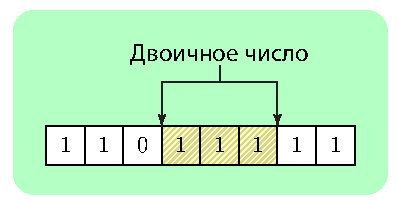
\includegraphics [scale=1] {TMHL_BinaryToDecimalFromPart_Sheme}
  \caption{Часть бинарной строки} 
  \label{img:TMHL_BinaryToDecimalFromPart_Sheme}  
\end{figure}
 
 \textbf{Примечание:}
 
 Для перевода всей бинарной строки в число лучше воспользоваться функцией TMHL\_BinaryToDecimal.

\textbf{Примечание:}

 Данная функция используется, например, если в бинарной строке закодировано несколько десятичных чисел, каждое из которых закодировано своей подстрокой, а общая строка получена склейкой этих бинарных строк.


\begin{lstlisting}[label=code_use_TMHL_BinaryToDecimalFromPart,caption=Пример использования]
        int VMHL_N=8;//Размер массива
        int *a;
        a=new int[VMHL_N];
        TMHL_RandomBinaryVector(a,VMHL_N);

        int Begin=2;

        //Вызов функции
        int x=TMHL_BinaryToDecimalFromPart(a,Begin,5);

        //Используем полученный результат
        MHL_ShowVectorT (a,VMHL_N,"Бинарная строка", "a");
        //Бинарная строка:
        //a =	
        //0	0	1	0	1	0	0	0
        
        MHL_ShowNumber (Begin,"Двоичное число состоит из 5 символов начиная с", "номера");
        //Двоичное число состоит из 5 символов начиная с:
        //номера=2
        
        MHL_ShowNumber (x,"Было закодировано", "x");
        //Было закодировано:
        //x=20
                
        delete [] a;
\end{lstlisting}

\subsubsection{TMHL\_GrayCodeToBinary}\label{TMHL_GrayCodeToBinary}

Функция переводит бинарный код Грея в бинарный код.


\begin{lstlisting}[label=code_syntax_TMHL_GrayCodeToBinary,caption=Синтаксис]
template <class T> void TMHL_GrayCodeToBinary(T *a,int *VMHL_ResultVector, int VMHL_N);
\end{lstlisting}

\textbf{Входные параметры:}
 
 a --- код Грея (массив заполнен 0 и 1);
 
 VMHL\_N --- длина массива a.
 
\textbf{Возвращаемое значение:}

 Отсутствует.
 
\textbf{О функции:}

Бинарная строка не представляет собой двоичный код целого числа, а представляет код Грея. Его отличительной особенностью является то, что если два целых числа отличаются на единицу, то их коды Грея также будут отличаться только одним битом. Двоичный код не обладает данным свойством.
Существует метод по переводу кода Грея в двоичный код: старший разряд (крайний левый бит) записывается без изменения, каждый следующий символ кода Грея нужно инвертировать, если в двоичном коде перед этим была получена «1», и оставить без изменения, если в двоичном коде был получен «0». 


\begin{lstlisting}[label=code_use_TMHL_GrayCodeToBinary,caption=Пример использования]
        int VMHL_N=5;//Размер массива
        int *GrayCode;
        GrayCode=new int[VMHL_N];
        //Получим случайный Грей код
        TMHL_RandomBinaryVector(GrayCode,VMHL_N);

        int *BinaryCode;
        BinaryCode=new int[VMHL_N];

        //Вызов функции
        TMHL_GrayCodeToBinary(GrayCode,BinaryCode,VMHL_N);

        //Используем полученный результат
        MHL_ShowVectorT (GrayCode,VMHL_N,"Грей код", "a");
        //Грей код:
        //a =
        //1	1	0	1	1

        MHL_ShowVectorT (BinaryCode,VMHL_N,"Бинарный код, полученый из кода Грея", "a");
        //Бинарный код, полученый из кода Грея:
        //a =
        //1	0	0	1	0

        delete [] GrayCode;
        delete [] BinaryCode;
\end{lstlisting}

\subsubsection{TMHL\_GrayCodeToBinaryFromPart}\label{TMHL_GrayCodeToBinaryFromPart}

Функция переводит бинарный код Грея в бинарный код. При этом бинарный код Грея берется как часть некой строки a, заполненной 0 и 1.


\begin{lstlisting}[label=code_syntax_TMHL_GrayCodeToBinaryFromPart,caption=Синтаксис]
template <class T> void TMHL_GrayCodeToBinaryFromPart(T *a, T *VMHL_ResultVector, int Begin, int n);
\end{lstlisting}

\textbf{Входные параметры:}
 
 a --- строка, заполненная 0 и 1;
 
 VMHL\_ResultVector --- сюда записывается вектор бинарного числа. Причем запись происходит в те же элементы по номерам, что брались из вектора a, то есть в номера элементов от Begin до Begin+n. Остальные элементы в VMHL\_ResultVector не трогаются.
 
 Begin --- номер элемента массива a как начало числа в виде кода Грея (начиная с нуля);
 
 n --- длина числа в виде кода Грея (это не длина вектора a).
 
\textbf{Возвращаемое значение:}

 Отсутствует.
 
\textbf{О функции:}

Для декодирования из строки кода Грея берется только часть:

\begin{figure} [h]
  \center
  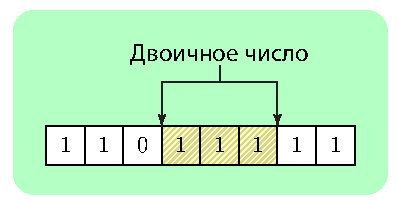
\includegraphics [scale=1] {TMHL_BinaryToDecimalFromPart_Sheme}
  \caption{Часть бинарной строки} 
  \label{img:TMHL_BinaryToDecimalFromPart_Sheme}  
\end{figure}

Бинарная подстрока не представляет собой двоичный код целого числа, а представляет код Грея. Его отличительной особенностью является то, что если два целых числа отличаются на единицу, то их коды Грея также будут отличаться только одним битом. Двоичный код не обладает данным свойством.

Существует метод по переводу кода Грея в двоичный код: старший разряд (крайний левый бит) записывается без изменения, каждый следующий символ кода Грея нужно инвертировать, если в двоичном коде перед этим была получена «1», и оставить без изменения, если в двоичном коде был получен «0».
 
 \textbf{Примечание:}
 
 Для перевода всей строки кода Грея в бинарную лучше воспользоваться функцией TMHL\_GrayCodeToBinary.

 \textbf{Примечание:}

 Для перевода полученной бинарной строки в десятичное число воспользуйтесь функцией TMHL\_BinaryToDecimal или TMHL\_BinaryToDecimalFromPart.

 \textbf{Примечание:}
 
 Данная функция используется, например, если в строке Грей кода закодировано несколько десятичных чисел, каждое из которых закодировано своей подстрокой, а общая строка получена склейкой этих строк Грей кода. Для того, чтобы получить десятичные числа проще вначале перевести Грей код в бинарный, а потом бинарный код перевести в десятичный.


\begin{lstlisting}[label=code_use_TMHL_GrayCodeToBinaryFromPart,caption=Пример использования]
        int VMHL_N=8;//Размер массива
        int *VectorWithGrayCode;
        VectorWithGrayCode=new int[VMHL_N];
        //Заполним случайно нулями и единицами
        TMHL_RandomBinaryVector(VectorWithGrayCode,VMHL_N);

        int *VectorWithBinaryCode;
        VectorWithBinaryCode=new int[VMHL_N];
        TMHL_FillVector(VectorWithBinaryCode,VMHL_N,-1);

        int Begin=2;

        //Вызов функции
        TMHL_GrayCodeToBinaryFromPart(VectorWithGrayCode,VectorWithBinaryCode,Begin,5);

        //Используем полученный результат
        MHL_ShowVectorT (VectorWithGrayCode,VMHL_N,"Строка, содержащая код Грея", "a");
        //Строка, содержащая код Грея:
        //a =	
        //1	0	0	1	1	1	0	0

        MHL_ShowNumber (Begin,"Двоичное число состоит из 5 символов начиная с", "номера");
        //Двоичное число состоит из 5 символов начиная с:
        //номера=2
        
        MHL_ShowVectorT (VectorWithBinaryCode,VMHL_N,"Строка, содержащая бинарный код, полученый из кода Грея", "a");
        //Строка, содержащая бинарный код, полученый из кода Грея:
        //a =	
        //-1	-1	0	1	0	1	1	-1

        delete [] VectorWithGrayCode;
        delete [] VectorWithBinaryCode;
\end{lstlisting}

\subsection{Комбинаторика}

\subsubsection{TMHL\_KCombinations}\label{TMHL_KCombinations}

Функция возвращает число сочетаний из n по m (без возвращения).


\begin{lstlisting}[label=code_syntax_TMHL_KCombinations,caption=Синтаксис]
template <class T> T TMHL_KCombinations(T k, T n);
\end{lstlisting}

\textbf{Входные параметры:}  
 
 k --- по сколько элементов надо брать в группу;
 
 n --- общее число элементов.

\textbf{Возвращаемое значение:}

 Число сочетаний из n по k.
 
 \textbf{Формула:}
 
 В программном коде число сочетаний находится через рекурсивную формулу. А в математике находится через формулу:
 
 \begin{equation*}
C_n^k=\dfrac{n!}{k!\left( n-k\right)! }.
\end{equation*}


\begin{lstlisting}[label=code_use_TMHL_KCombinations,caption=Пример использования]
        int n=10;
        int k=MHL_RandomUniformInt(0,10);

        int C=TMHL_KCombinations(k,n);

        //Используем полученный результат
        MHL_ShowNumber(C,"Число сочетаний по "+MHL_NumberToText(k)+" элементов из " +MHL_NumberToText(n),"C");
        //Число сочетаний по 8 элементов из 10:
        //C=45
\end{lstlisting}

\subsection{Математические функции}

\subsubsection{MHL\_ArithmeticalProgression}\label{MHL_ArithmeticalProgression}

Арифметическая прогрессия. n-ый член последовательности.


\begin{lstlisting}[label=code_syntax_MHL_ArithmeticalProgression,caption=Синтаксис]
double MHL_ArithmeticalProgression(double a1,double d,int n);
\end{lstlisting}

\textbf{Входные параметры:}  
 
a1 --- начальный член прогрессии;
 
d --- шаг арифметической прогрессии;
 
n --- номер последнего члена.

\textbf{Возвращаемое значение:}
 
n-ый член последовательности.


\begin{lstlisting}[label=code_use_MHL_ArithmeticalProgression,caption=Пример использования]
        double a1=MHL_RandomUniformInt(1,10);
        double d=MHL_RandomUniformInt(1,10);
        int n=MHL_RandomUniformInt(1,10);

        double an=MHL_ArithmeticalProgression(a1,d,n);

        //Используем полученный результат
        MHL_ShowNumber(a1,"Первый член последовательности","a1");
        //Первый член последовательности:
        //a1=6
        MHL_ShowNumber(d,"Шаг арифметической прогрессии","d");
        //Шаг арифметической прогрессии:
        //d=9
        MHL_ShowNumber(n,"Номер последнего члена","n");
        //Номер последнего члена:
        //n=4
        MHL_ShowNumber(an,"n-ый член последовательности","an");
        //n-ый член последовательности:
        //an=33
\end{lstlisting}

\subsubsection{MHL\_ExpMSxD2}\label{MHL_ExpMSxD2}

Функция вычисляет выражение $exp(-x*x/2)$.


\begin{lstlisting}[label=code_syntax_MHL_ExpMSxD2,caption=Синтаксис]
double MHL_ExpMSxD2(double x);
\end{lstlisting}

\textbf{Входные параметры:}

 x --- входная переменная.

\textbf{Возвращаемое значение:}
 
 Значение функции в точке.
 
\textbf{Формула:}
\begin{equation*}
F\left(x \right)=e^{-\dfrac{x^2}{2}}.
\end{equation*}

 \begin{figure} [h] 
   \center
   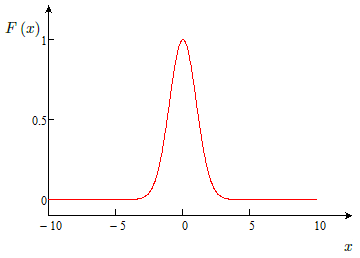
\includegraphics {MHL_ExpMSxD2_Graph.png}
   \caption{График функции} 
   \label{img:MHL_ExpMSxD2_Graph}  
 \end{figure}
 



\begin{lstlisting}[label=code_use_MHL_ExpMSxD2,caption=Пример использования]
        double t;
        double f;
        t=MHL_RandomUniform(0,3);

        //Вызов функции
        f=MHL_ExpMSxD2(t);

        //Используем полученный результат

        MHL_ShowNumber (t,"Параметр", "t");
        //Параметр:
        //t=2.06177
        MHL_ShowNumber (f,"Значение функции", "f");
        //Значение функции:
        //f=0.11938
\end{lstlisting}

\subsubsection{MHL\_GeometricSeries}\label{MHL_GeometricSeries}

Геометрическая прогрессия. n-ый член последовательности.


\begin{lstlisting}[label=code_syntax_MHL_GeometricSeries,caption=Синтаксис]
double MHL_GeometricSeries(double u1,double q,int n);
\end{lstlisting}

\textbf{Входные параметры:}  
 
u1 --- начальный член прогрессии;
 
q --- шаг  прогрессии;
 
n --- номер последнего члена.

\textbf{Возвращаемое значение:}
 
n-ый член последовательности.


\begin{lstlisting}[label=code_use_MHL_GeometricSeries,caption=Пример использования]
        double u1=MHL_RandomUniformInt(1,10);
        double q=MHL_RandomUniformInt(1,10);
        int n=MHL_RandomUniformInt(1,10);

        double qn=MHL_GeometricSeries(u1,q,n);

        //Используем полученный результат
        MHL_ShowNumber(u1,"Первый член последовательности","u1");
        //Первый член последовательности:
        //u1=4
        MHL_ShowNumber(q,"Шаг арифметической прогрессии","q");
        //Шаг арифметической прогрессии:
        //q=4
        MHL_ShowNumber(n,"Номер последнего члена","n");
        //Номер последнего члена:
        //n=6
        MHL_ShowNumber(qn,"n-ый член последовательности","qn");
        //n-ый член последовательности:
        //qn=4096
\end{lstlisting}

\subsubsection{MHL\_GreatestCommonDivisorEuclid}\label{MHL_GreatestCommonDivisorEuclid}

Функция находит наибольший общий делитель двух чисел по алгоритму Евклида.


\begin{lstlisting}[label=code_syntax_MHL_GreatestCommonDivisorEuclid,caption=Синтаксис]
int MHL_GreatestCommonDivisorEuclid(int A,int B);
\end{lstlisting}

\textbf{Входные параметры:}  
 
A --- первое число;
 
B --- второе число.

\textbf{Возвращаемое значение:}
 
НОД(A,B)


\begin{lstlisting}[label=code_use_MHL_GreatestCommonDivisorEuclid,caption=Пример использования]
        int A=MHL_RandomUniformInt(1,100);
        int B=MHL_RandomUniformInt(1,100);

        double Result=MHL_GreatestCommonDivisorEuclid(A,B);

        //Используем полученный результат
        MHL_ShowNumber(A,"Число","A");
        //Число:
        //A=96
        MHL_ShowNumber(B,"Число","B");
        //Число:
        //B=18
        MHL_ShowNumber(Result,"НОД","");
        //НОД:
        //=6
\end{lstlisting}

\subsubsection{MHL\_HowManyPowersOfTwo}\label{MHL_HowManyPowersOfTwo}

Функция вычисляет, какой минимальной степенью двойки можно покрыть целое положительное число.


\begin{lstlisting}[label=code_syntax_MHL_HowManyPowersOfTwo,caption=Синтаксис]
int MHL_HowManyPowersOfTwo(int x);
\end{lstlisting}

\textbf{Входные параметры:}  
 
x --- целое число.

\textbf{Возвращаемое значение:}
 
 Минимальная степень двойки можно покрыть целое положительное число: $2^{VMHL\_Result}>x$


\begin{lstlisting}[label=code_use_MHL_HowManyPowersOfTwo,caption=Пример использования]
        int x=MHL_RandomUniformInt(0,1000);
        int Degree;

        //Вызываем функцию
        Degree=MHL_HowManyPowersOfTwo(x);

        //Используем полученный результат
        MHL_ShowNumber(x,"Число","x");
        //Число:
        //x=480
        MHL_ShowNumber(Degree,"Его покрывает 2 в степени","Degree");
        //Его покрывает 2 в степени:
        //Degree=9
        MHL_ShowNumber(TMHL_PowerOf(2,Degree),"То есть","2^"+MHL_NumberToText(Degree));
        //То есть:
        //2^9=512
\end{lstlisting}

\subsubsection{MHL\_InverseNormalizationNumberAll}\label{MHL_InverseNormalizationNumberAll}

Функция осуществляет обратную нормировку числа из интервала $\left[0;1\right] $  в интервал $\left[-\infty;\infty \right] $, которое было осуществлено функцией MHL\_NormalizationNumberAll.


\begin{lstlisting}[label=code_syntax_MHL_InverseNormalizationNumberAll,caption=Синтаксис]
double MHL_InverseNormalizationNumberAll(double x);
\end{lstlisting}

\textbf{Входные параметры:}

 x --- число в интервале [0;1].

\textbf{Возвращаемое значение:}
 
Перенормированное число.


\begin{lstlisting}[label=code_use_MHL_InverseNormalizationNumberAll,caption=Пример использования]
        double x;
        double y;
        x=MHL_RandomNumber();

        //Вызов функции
        y=MHL_InverseNormalizationNumberAll(x);

        //Используем полученный результат
        MHL_ShowNumber (x,"Нормированное число", "x");
        // Нормированное число:
        //x=0.0491333
        MHL_ShowNumber (y,"Перенормированное число", "y");
        // Перенормированное число:
        //y=-9.1764
\end{lstlisting}

\subsubsection{MHL\_LeastCommonMultipleEuclid}\label{MHL_LeastCommonMultipleEuclid}

Функция находит наименьшее общее кратное двух чисел по алгоритму Евклида.


\begin{lstlisting}[label=code_syntax_MHL_LeastCommonMultipleEuclid,caption=Синтаксис]
int MHL_LeastCommonMultipleEuclid(int A,int B);
\end{lstlisting}

\textbf{Входные параметры:}  
 
A --- первое число;
 
B --- второе число.

\textbf{Возвращаемое значение:}
 
 НОК(A,B)


\begin{lstlisting}[label=code_use_MHL_LeastCommonMultipleEuclid,caption=Пример использования]
        int A=MHL_RandomUniformInt(1,100);
        int B=MHL_RandomUniformInt(1,100);

        double Result=MHL_LeastCommonMultipleEuclid(A,B);

        //Используем полученный результат
        MHL_ShowNumber(A,"Число","A");
        //Число:
        //A=68
        MHL_ShowNumber(B,"Число","B");
        //Число:
        //B=67
        MHL_ShowNumber(Result,"НОК","");
        //НОК:
        //=4556
\end{lstlisting}

\subsubsection{MHL\_NormalizationNumberAll}\label{MHL_NormalizationNumberAll}

Функция нормирует число из интервала $\left[-\infty;\infty \right] $ в интервал $\left[0;1\right]$. При этом в нуле возвращает $0.5$, в $-\infty$ возвращает $0$, в $\infty$ возвращает $1$. Если $x<y$, то $MHL\_NormalizationNumberAll(x)<MHL\_NormalizationNumberAll(y)$. Под бесконечностью принимается машинная бесконечность.


\begin{lstlisting}[label=code_syntax_MHL_NormalizationNumberAll,caption=Синтаксис]
double MHL_NormalizationNumberAll(double x);
\end{lstlisting}

\textbf{Входные параметры:}

 x --- число.

\textbf{Возвращаемое значение:}
 
Нормированное число.
 
\textbf{Формула:}
\begin{equation*}
f\left(x \right)=\frac{1}{2}\left( \dfrac{1}{1+\dfrac{1}{\left| x\right| }}\cdot sign \left( x\right)+1 \right) .
\end{equation*}


\begin{lstlisting}[label=code_use_MHL_NormalizationNumberAll,caption=Пример использования]
        double x;
        double y;
        y=MHL_RandomUniform(-100,100);

        //Вызов функции
        x=MHL_NormalizationNumberAll(y);

        //Используем полученный результат
        MHL_ShowNumber (y,"Число", "y");
        //Число:
        //y=-10.4004
        MHL_ShowNumber (x,"Нормированное число", "x");
        //Нормированное число:
        //x=0.0438581
\end{lstlisting}

\subsubsection{MHL\_Parity}\label{MHL_Parity}

Функция проверяет четность целого числа.


\begin{lstlisting}[label=code_syntax_MHL_Parity,caption=Синтаксис]
int MHL_Parity(int a);
\end{lstlisting}

\textbf{Входные параметры:}  
 
a --- исходное число.

\textbf{Возвращаемое значение:}

 1 --- четное;
 
 0 --- нечетное.


\begin{lstlisting}[label=code_use_MHL_Parity,caption=Пример использования]
        int a=MHL_RandomUniformInt(-50,50);

        double Result=MHL_Parity(a);

        //Используем полученный результат
        MHL_ShowNumber(Result,"Четность числа "+MHL_NumberToText(a),"равна");
        //Четность числа 2:
        //равна=1
\end{lstlisting}

\subsubsection{MHL\_SumGeometricSeries}\label{MHL_SumGeometricSeries}

Геометрическая прогрессия. Сумма первых n членов.


\begin{lstlisting}[label=code_syntax_MHL_SumGeometricSeries,caption=Синтаксис]
double MHL_SumGeometricSeries(double u1,double q,int n);
\end{lstlisting}

\textbf{Входные параметры:}  
 
u1 --- начальный член прогрессии;
 
q --- шаг  прогрессии;
 
n --- номер последнего члена.

\textbf{Возвращаемое значение:}
 
Сумма первых n членов.


\begin{lstlisting}[label=code_use_MHL_SumGeometricSeries,caption=Пример использования]
        double u1=MHL_RandomUniformInt(1,5);
        double q=MHL_RandomUniformInt(1,5);
        int n=MHL_RandomUniformInt(1,5);

        double Sum=MHL_SumGeometricSeries(u1,q,n);

        //Используем полученный результат
        MHL_ShowNumber(u1,"Первый член последовательности","u1");
        //Первый член последовательности:
        //u1=4
        MHL_ShowNumber(q,"Шаг арифметической прогрессии","q");
        //Шаг арифметической прогрессии:
        //q=4
        MHL_ShowNumber(n,"Номер последнего члена","n");
        //Номер последнего члена:
        //n=3
        MHL_ShowNumber(Sum,"Сумма первых n членов","Sum");
        //Сумма первых n членов:
        //Sum=84
\end{lstlisting}

\subsubsection{MHL\_SumOfArithmeticalProgression}\label{MHL_SumOfArithmeticalProgression}

Арифметическая прогрессия. Сумма первых n членов.


\begin{lstlisting}[label=code_syntax_MHL_SumOfArithmeticalProgression,caption=Синтаксис]
double MHL_SumOfArithmeticalProgression(double a1,double d,int n);
\end{lstlisting}

\textbf{Входные параметры:}  
 
 a1 --- начальный член прогрессии;
 
 d --- шаг арифметической прогрессии;
 
 n --- номер последнего члена.

\textbf{Возвращаемое значение:}
 
Сумма первых n членов.


\begin{lstlisting}[label=code_use_MHL_SumOfArithmeticalProgression,caption=Пример использования]
        double a1=MHL_RandomUniformInt(1,10);
        double d=MHL_RandomUniformInt(1,10);
        int n=MHL_RandomUniformInt(1,10);

        double Sum=MHL_SumOfArithmeticalProgression(a1,d,n);

        //Используем полученный результат
        MHL_ShowNumber(a1,"Первый член последовательности","a1");
        //Первый член последовательности:
        //a1=9
        MHL_ShowNumber(d,"Шаг арифметической прогрессии","d");
        //Шаг арифметической прогрессии:
        //d=6
        MHL_ShowNumber(n,"Номер последнего члена","n");
        //Номер последнего члена:
        //n=9
        MHL_ShowNumber(Sum,"Сумма первых n членов","Sum");
        //Сумма первых n членов:
        //Sum=297
\end{lstlisting}

\subsubsection{MHL\_SumOfDigits}\label{MHL_SumOfDigits}

Функция подсчитывает сумму цифр любого целого числа.


\begin{lstlisting}[label=code_syntax_MHL_SumOfDigits,caption=Синтаксис]
int MHL_SumOfDigits(int a);
\end{lstlisting}

\textbf{Входные параметры:}

a --- целое число.

\textbf{Возвращаемое значение:}

Cумма цифр.


\begin{lstlisting}[label=code_use_MHL_SumOfDigits,caption=Пример использования]
        int a=MHL_RandomUniformInt(100,30000);

        //Вызов функции
        int SumOfDigits=MHL_SumOfDigits(a);

        //Используем полученный результат
        MHL_ShowNumber (SumOfDigits,"Сумма цифр числа a="+MHL_NumberToText(a), "равна");
        //Сумма цифр числа a=2069:
        //равна=17
\end{lstlisting}

\subsubsection{TMHL\_Abs}\label{TMHL_Abs}

Функция возвращает модуль числа.


\begin{lstlisting}[label=code_syntax_TMHL_Abs,caption=Синтаксис]
template <class T> T TMHL_Abs(T x);
\end{lstlisting}

\textbf{Входные параметры:}

 x --- число.
 
\textbf{Возвращаемое значение:}

 Модуль числа.


\begin{lstlisting}[label=code_use_TMHL_Abs,caption=Пример использования]
        double x;
        double abs;

        x=MHL_RandomUniform(-10,10);

        //Вызов функции
        abs=TMHL_Abs(x);

        //Используем полученный результат
        MHL_ShowNumber (x,"Число", "x");
        // Число:
        //x=-6.29578
        MHL_ShowNumber (abs,"Модуль", "abs");
        // Модуль:
        //abs=6.29578
\end{lstlisting}

\subsubsection{TMHL\_Factorial}\label{TMHL_Factorial}

Функция вычисляет факториал числа.


\begin{lstlisting}[label=code_syntax_TMHL_Factorial,caption=Синтаксис]
template <class T> T TMHL_Factorial(T x);
\end{lstlisting}

\textbf{Входные параметры:}  
 
 x --- число.

\textbf{Возвращаемое значение:}

 Факториал числа.


\begin{lstlisting}[label=code_use_TMHL_Factorial,caption=Пример использования]
        int a=MHL_RandomUniformInt(0,10);

        double Result=TMHL_Factorial(a);

        //Используем полученный результат
        MHL_ShowNumber(Result,"Факториал числа "+MHL_NumberToText(a),"a!");
        //Факториал числа 3:
        //a!=6
\end{lstlisting}

\subsubsection{TMHL\_FibonacciNumber}\label{TMHL_FibonacciNumber}

Функция вычисляет число Фибоначчи, заданного номера.


\begin{lstlisting}[label=code_syntax_TMHL_FibonacciNumber,caption=Синтаксис]
template <class T> T TMHL_FibonacciNumber(T n);
\end{lstlisting}

\textbf{Входные параметры:}  
 
 n --- номер числа Фибоначчи.

\textbf{Возвращаемое значение:}
 
 Число Фибоначчи, заданного номера.


\begin{lstlisting}[label=code_use_TMHL_FibonacciNumber,caption=Пример использования]
        int n;
        int F;
        n=MHL_RandomUniformInt(3,20);

        //Вызов функции
        F=TMHL_FibonacciNumber(n);

        //Используем полученный результат

        MHL_ShowNumber (n,"Номер числа", "n");
        // Номер числа:
        // n=14
        MHL_ShowNumber (F,"Число Фибоначчи, заданного номера", "F");
        // Число Фибоначчи, заданного номера:
        // F=377
\end{lstlisting}

\subsubsection{TMHL\_HeavisideFunction}\label{TMHL_HeavisideFunction}

Функция Хевисайда (функция одной переменной).


\begin{lstlisting}[label=code_syntax_TMHL_HeavisideFunction,caption=Синтаксис]
template <class T> T TMHL_HeavisideFunction(T x);
\end{lstlisting}

\textbf{Входные параметры:}

 x --- переменная.

\textbf{Возвращаемое значение:}
 
 Значение функции Хевисайда.
 
\textbf{Формула:}
\begin{equation*}
F\left(x \right)=\left\lbrace \begin{aligned}
1&\text{, если } x>0; \\
0&\text{, если } x\leq 0.
\end{aligned}\right. 
\end{equation*}

 \begin{figure} [h] 
   \center
   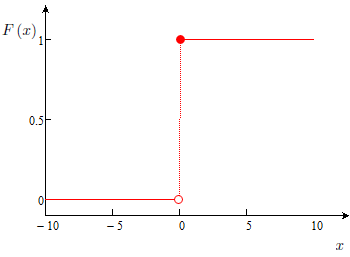
\includegraphics {TMHL_HeavisideFunction_Graph.png}
   \caption{График функции} 
   \label{img:TMHL_HeavisideFunction_Graph}  
 \end{figure}
 



\begin{lstlisting}[label=code_use_TMHL_HeavisideFunction,caption=Пример использования]
        double x=MHL_RandomUniform(-50,50);

        double F=TMHL_HeavisideFunction(x);

        //Используем полученный результат
        MHL_ShowNumber(F,"Функция Хэвисайда при a = "+MHL_NumberToText(x),"равна");
        //Функция Хэвисайда при a = -49.7559:
        //равна=0
\end{lstlisting}

\subsubsection{TMHL\_Max}\label{TMHL_Max}

Функция возвращает максимальный элемент из двух.


\begin{lstlisting}[label=code_syntax_TMHL_Max,caption=Синтаксис]
template <class T> T TMHL_Max(T a, T b);
\end{lstlisting}

\textbf{Входные параметры:}

 a --- первый элемент;
	
 b --- первый элемент.


\textbf{Возвращаемое значение:}

Максимальный элемент.


\begin{lstlisting}[label=code_use_TMHL_Max,caption=Пример использования]
        int a=MHL_RandomUniformInt(10,100);
        int b=MHL_RandomUniformInt(10,100);

        //Вызов функции
        int Max=TMHL_Max(a,b);

        //Используем полученный результат
        MHL_ShowNumber(Max,"Максимальное среди "+MHL_NumberToText(a)+" и "+MHL_NumberToText(b),"равно");
        //Максимальное среди 73 и 44:
        //равно=73
\end{lstlisting}

\subsubsection{TMHL\_Min}\label{TMHL_Min}

Функция возвращает минимальный элемент из двух.


\begin{lstlisting}[label=code_syntax_TMHL_Min,caption=Синтаксис]
template <class T> T TMHL_Min(T a, T b);
\end{lstlisting}

\textbf{Входные параметры:}

 a --- первый элемент;
	
 b --- первый элемент.

\textbf{Возвращаемое значение:}

Минимальный элемент.


\begin{lstlisting}[label=code_use_TMHL_Min,caption=Пример использования]
        int a=MHL_RandomUniformInt(10,100);
        int b=MHL_RandomUniformInt(10,100);

        //Вызов функции
        int Max=TMHL_Min(a,b);

        //Используем полученный результат
        MHL_ShowNumber(Max,"Минимальное среди "+MHL_NumberToText(a)+" и "+MHL_NumberToText(b),"равно");
        //Минимальное среди 79 и 18:
        //равно=18
\end{lstlisting}

\subsubsection{TMHL\_NumberInterchange}\label{TMHL_NumberInterchange}

Функция меняет местами значения двух чисел.


\begin{lstlisting}[label=code_syntax_TMHL_NumberInterchange,caption=Синтаксис]
template <class T> void TMHL_NumberInterchange(T *a, T *b);
\end{lstlisting}

\textbf{Входные параметры:}

 a --- первое число;
 
 b --- второе число.

\textbf{Возвращаемое значение:}

 Отсутствует.


\begin{lstlisting}[label=code_use_TMHL_NumberInterchange,caption=Пример использования]
        double a=MHL_RandomUniform(-10,10);
        double b=MHL_RandomUniform(-10,10);

        MHL_ShowNumber(a,"Было","a");
        //Было:
        //a=-3.18237
        MHL_ShowNumber(b,"Было","b");
        //Было:
        //b=5.36194

        //Вызов функции
        TMHL_NumberInterchange(&a,&b);

        //Используем полученный результат
        MHL_ShowNumber(a,"Стало","a");
        //Стало:
        //a=5.36194
        MHL_ShowNumber(b,"Стало","b");
        //Стало:
        //b=-3.18237
\end{lstlisting}

\subsubsection{TMHL\_PowerOf}\label{TMHL_PowerOf}

Функция возводит произвольное число в целую степень.


\begin{lstlisting}[label=code_syntax_TMHL_PowerOf,caption=Синтаксис]
template <class T> T TMHL_PowerOf(T x, int n);
\end{lstlisting}

\textbf{Входные параметры:}  
 
x --- основание степени;
 
n --- показатель степени.

\textbf{Возвращаемое значение:}

Cтепень числа.


\begin{lstlisting}[label=code_use_TMHL_PowerOf,caption=Пример использования]
        double a=MHL_RandomUniform(-5,5);
        int Degree=MHL_RandomUniformInt(0,20);

        double Result=TMHL_PowerOf(a,Degree);

        //Используем полученный результат
        MHL_ShowNumber(Result,"Число "+MHL_NumberToText(a)+" в степени "+MHL_NumberToText(Degree),"равно");
        //Число 3.9624 в степени 4:
        //равно=246.51
\end{lstlisting}

\subsubsection{TMHL\_Sign}\label{TMHL_Sign}

Функция вычисляет знака числа.


\begin{lstlisting}[label=code_syntax_TMHL_Sign,caption=Синтаксис]
template <class T> int TMHL_Sign(T a);
\end{lstlisting}

\textbf{Входные параметры:}

 a --- исходное число.

\textbf{Возвращаемое значение:}

 0 --- если a==0;
 
 1 --- если число положительное;
 
 -1 --- если число отрицательное.


\begin{lstlisting}[label=code_use_TMHL_Sign,caption=Пример использования]
        int a=MHL_RandomUniformInt(-5,5);

        //Вызов функции
        int Result=TMHL_Sign(a);

        //Используем полученный результат
        MHL_ShowNumber(Result,"Знак числа "+MHL_NumberToText(a),"равен");
        //Знак числа -3:
        //равен=-1
\end{lstlisting}

\subsubsection{TMHL\_SignNull}\label{TMHL_SignNull}

Функция вычисляет знака числа. При нуле возвращает 1.


\begin{lstlisting}[label=code_syntax_TMHL_SignNull,caption=Синтаксис]
template <class T> int TMHL_SignNull(T a);
\end{lstlisting}

\textbf{Входные параметры:}

 a --- исходное число.

\textbf{Возвращаемое значение:}

 1 --- если число неотрицательное;
 
 -1 --- если число отрицательное.


\begin{lstlisting}[label=code_use_TMHL_SignNull,caption=Пример использования]
        int a=MHL_RandomUniformInt(-5,5);

        //Вызов функции
        int Result=TMHL_SignNull(a);

        //Используем полученный результат
        MHL_ShowNumber(Result,"Знак числа "+MHL_NumberToText(a),"равен");
        //Знак числа 0:
        //равен=1
\end{lstlisting}

\subsection{Матрицы}

\subsubsection{TMHL\_ColInterchange}\label{TMHL_ColInterchange}

Функция переставляет столбцы матрицы.


\begin{lstlisting}[label=code_syntax_TMHL_ColInterchange,caption=Синтаксис]
template <class T> void TMHL_ColInterchange(T **VMHL_ResultMatrix, int VMHL_N, int k, int l);
\end{lstlisting}

\textbf{Входные параметры:} 
 
VMHL\_ResultMatrix --- указатель на исходную матрицу (в ней и сохраняется результат);
 
VMHL\_N --- размер массива (число строки);
 
k,l --- номера переставляемых столбцов (нумерация с нуля).

\textbf{Возвращаемое значение:}

Отсутствует.


\begin{lstlisting}[label=code_use_TMHL_ColInterchange,caption=Пример использования]
        int i,j;
        int VMHL_N=5;//Размер массива (число строк)
        int VMHL_M=5;//Размер массива (число столбцов)
        int **Matrix;
        Matrix=new int*[VMHL_N];
        for (i=0;i<VMHL_N;i++) Matrix[i]=new int[VMHL_M];
        //Заполним случайными числами
        for (i=0;i<VMHL_N;i++)
         for (j=0;j<VMHL_M;j++)
          Matrix[i][j]=MHL_RandomUniformInt(10,100);

        MHL_ShowMatrix (Matrix,VMHL_N,VMHL_M,"Случайная матрица", "Matrix");
        // Случайная матрица:
        //Matrix =	
        //46	37	90	95	83
        //92	58	48	61	16
        //31	92	37	64	56
        //20	54	84	90	75
        //86	79	20	40	69

        // номера перставляемых столбцов
        int k=MHL_RandomUniformInt(0,5);
        int l=MHL_RandomUniformInt(0,5);

        //Вызов функции
        TMHL_ColInterchange(Matrix,VMHL_N,k,l);

        //Используем полученный результат
        MHL_ShowNumber (k,"Номер первого столбца","k");
        // Номер первого столбца:
        //k=4
        MHL_ShowNumber (l,"Номер второго столбца","l");
        // Номер второго столбца:
        //l=0
        MHL_ShowMatrix (Matrix,VMHL_N,VMHL_M,"Матрица с персетавленными столбцами", "Matrix");
        // Матрица с персетавленными столбцами:
        //Matrix =	
        //83	37	90	95	46
        //16	58	48	61	92
        //56	92	37	64	31
        //75	54	84	90	20
        //69	79	20	40	86

        for (i=0;i<VMHL_N;i++) delete [] Matrix[i];
        delete [] Matrix;
\end{lstlisting}

\subsubsection{TMHL\_ColToMatrix}\label{TMHL_ColToMatrix}

Функция копирует в матрицу (двумерный массив) из вектора столбец.


\begin{lstlisting}[label=code_syntax_TMHL_ColToMatrix,caption=Синтаксис]
template <class T> void TMHL_ColToMatrix(T **VMHL_ResultMatrix, T *b, int VMHL_N, int k);
\end{lstlisting}

\textbf{Входные параметры:}  
 
VMHL\_ResultMatrix --- указатель на матрицу;
 
b --- указатель на вектор;
 
VMHL\_N --- количество строк в матрице и одновременно размер массива b;
 
k --- номер столбца, в который будет происходить копирование (начиная с 0).

\textbf{Возвращаемое значение:}

Отсутствует.


\begin{lstlisting}[label=code_use_TMHL_ColToMatrix,caption=Пример использования]
        int i,j;
        int VMHL_N=10;//Размер массива (число строк)
        int VMHL_M=3;//Размер массива (число столбцов)
        int **a;
        a=new int*[VMHL_N];
        for (i=0;i<VMHL_N;i++) a[i]=new int[VMHL_M];
        int *b;
        b=new int[VMHL_N];
        //Заполним случайными числами
        for (i=0;i<VMHL_N;i++)
         for (j=0;j<VMHL_M;j++)
          a[i][j]=MHL_RandomUniformInt(10,100);
        MHL_ShowMatrix (a,VMHL_N,VMHL_M,"Случайная матрица", "a");
        //Случайная матрица:
        //a =
        //13	99	23
        //69	44	44
        //64	70	72
        //14	85	92
        //11	40	12
        //95	85	81
        //82	50	13
        //63	82	58
        //56	68	89
        //51	89	78

        for (j=0;j<VMHL_N;j++)
         b[j]=MHL_RandomUniformInt(10,100);

        int k=1;//Номер столбца, в который мы копируем

        //Вызов функции
        TMHL_ColToMatrix(a,b,VMHL_N,k);

        //Используем полученный результат
        MHL_ShowNumber(k,"Номер столбца, в который мы копируем ","k");
        //Номер столбца, в который мы копируем :
        //k=1
        MHL_ShowVector (b,VMHL_N,"Вектор","b");
        //Вектор:
        //b =
        //35
        //92
        //90
        //41
        //17
        //24
        //11
        //13
        //23
        //14

        MHL_ShowMatrix (a,VMHL_N,VMHL_M,"Матрица с изменившимся столбцом", "a");
        //Матрица с изменившимся столбцом:
        //a =
        //13	35	23
        //69	92	44
        //64	90	72
        //14	41	92
        //11	17	12
        //95	24	81
        //82	11	13
        //63	13	58
        //56	23	89
        //51	14	78

        for (i=0;i<VMHL_N;i++) delete [] a[i];
        delete [] a;
        delete [] b;
\end{lstlisting}

\subsubsection{TMHL\_DeleteColInMatrix}\label{TMHL_DeleteColInMatrix}

Функция удаляет k столбец из матрицы (начиная с нуля). Все правостоящие столбцы сдвигаются влево  на единицу. Последний столбец зануляется.


\begin{lstlisting}[label=code_syntax_TMHL_DeleteColInMatrix,caption=Синтаксис]
template <class T> void TMHL_DeleteColInMatrix(T **VMHL_ResultMatrix, int k, int VMHL_N, int VMHL_M);
\end{lstlisting}

\textbf{Входные параметры:}  
 
VMHL\_ResultMatrix --- указатель на преобразуемый массив;
 
k --- номер удаляемого столбца;
 
VMHL\_N --- размер массива VMHL\_ResultMatrix (число строк);
 
VMHL\_M --- размер массива VMHL\_ResultMatrix (число столбцов).

\textbf{Возвращаемое значение:}

Отсутствует.


\begin{lstlisting}[label=code_use_TMHL_DeleteColInMatrix,caption=Пример использования]
        int i,j;
        int VMHL_N=6;//Размер массива (число строк)
        int VMHL_M=4;//Размер массива (число столбцов)
        double **Matrix;
        Matrix=new double*[VMHL_N];
        for (i=0;i<VMHL_N;i++) Matrix[i]=new double[VMHL_M];
        //Заполним случайными числами
        for (i=0;i<VMHL_N;i++)
         for (j=0;j<VMHL_M;j++)
          Matrix[i][j]=MHL_RandomUniformInt(10,100);

        MHL_ShowMatrix (Matrix,VMHL_N,VMHL_M,"Случайная матрица", "Matrix");
        // Случайная матрица:
        //Matrix =
        //39	52	14	31
        //49	49	59	65
        //68	15	12	86
        //91	73	36	32
        //52	31	24	78
        //22	20	33	94

        int k=2;//Удалим второй столбец

        //Вызов функции
        TMHL_DeleteColInMatrix(Matrix,k,VMHL_N,VMHL_M);

        //Используем полученный результат

        MHL_ShowMatrix (Matrix,VMHL_N,VMHL_M,"Матрица с удаленным столбцом", "Matrix");
        // Матрица с удаленным столбцом:
        //Matrix =
        //39	52	31	0
        //49	49	65	0
        //68	15	86	0
        //91	73	32	0
        //52	31	78	0
        //22	20	94	0

        for (i=0;i<VMHL_N;i++) delete [] Matrix[i];
        delete [] Matrix;
\end{lstlisting}

\subsubsection{TMHL\_DeleteRowInMatrix}\label{TMHL_DeleteRowInMatrix}

Функция удаляет k строку из матрицы (начиная с нуля). Все нижестоящие строки поднимаются на единицу. Последняя строка зануляется.


\begin{lstlisting}[label=code_syntax_TMHL_DeleteRowInMatrix,caption=Синтаксис]
template <class T> void TMHL_DeleteRowInMatrix(T **VMHL_ResultMatrix, int k, int VMHL_N, int VMHL_M);
\end{lstlisting}

\textbf{Входные параметры:}  
 
VMHL\_ResultMatrix --- указатель на преобразуемый массив;
 
k --- номер удаляемой строки;
 
VMHL\_N --- размер массива VMHL\_ResultMatrix (число строк);
 
VMHL\_M --- размер массива VMHL\_ResultMatrix (число столбцов).

\textbf{Возвращаемое значение:}

Отсутствует.


\begin{lstlisting}[label=code_use_TMHL_DeleteRowInMatrix,caption=Пример использования]
        int i,j;
        int VMHL_N=6;//Размер массива (число строк)
        int VMHL_M=4;//Размер массива (число столбцов)
        double **Matrix;
        Matrix=new double*[VMHL_N];
        for (i=0;i<VMHL_N;i++) Matrix[i]=new double[VMHL_M];
        //Заполним случайными числами
        for (i=0;i<VMHL_N;i++)
         for (j=0;j<VMHL_M;j++)
          Matrix[i][j]=MHL_RandomUniformInt(10,100);

        MHL_ShowMatrix (Matrix,VMHL_N,VMHL_M,"Случайная матрица", "Matrix");
        // Случайная матрица:
        //Matrix =
        //70	57	44	95
        //26	21	60	63
        //61	55	27	95
        //10	10	43	92
        //66	20	51	65
        //32	52	63	78

        int k=2;//Удалим вторую строку

        //Вызов функции
        TMHL_DeleteRowInMatrix(Matrix,k,VMHL_N,VMHL_M);

        //Используем полученный результат

        MHL_ShowMatrix (Matrix,VMHL_N,VMHL_M,"Матрица с удаленной строкой", "Matrix");
        // Матрица с удаленной строкой:
        //Matrix =
        //70	57	44	95
        //26	21	60	63
        //10	10	43	92
        //66	20	51	65
        //32	52	63	78
        //0	0	0	0

        for (i=0;i<VMHL_N;i++) delete [] Matrix[i];
        delete [] Matrix;
\end{lstlisting}

\subsubsection{TMHL\_FillMatrix}\label{TMHL_FillMatrix}

Функция заполняет матрицу значениями, равных x.


\begin{lstlisting}[label=code_syntax_TMHL_FillMatrix,caption=Синтаксис]
template <class T> void TMHL_FillMatrix(T **VMHL_ResultMatrix, int VMHL_N, int VMHL_M, T x);
\end{lstlisting}

\textbf{Входные параметры:}

 VMHL\_ResultMatrix --- указатель на преобразуемый массив;
 
 VMHL\_N --- размер массива VMHL\_ResultMatrix (число строк);
 
 VMHL\_M --- размер массива VMHL\_ResultMatrix (число столбцов);

\textbf{Возвращаемое значение:}

Отсутствует.


\begin{lstlisting}[label=code_use_TMHL_FillMatrix,caption=Пример использования]
        int i;
        int VMHL_N=10;//Размер массива (число строк)
        int VMHL_M=3;//Размер массива (число столбцов)
        int **a;
        a=new int*[VMHL_N];
        for (i=0;i<VMHL_N;i++) a[i]=new int[VMHL_M];

        int x=MHL_RandomUniformInt(0,10);//заполнитель

        //Вызов функции
        TMHL_FillMatrix(a,VMHL_N,VMHL_M,x);

        //Используем полученный результат
        MHL_ShowMatrix (a,VMHL_N,VMHL_M,"Заполненная матрица", "a");
        //Заполненная матрица:
        //a =	
        //3	3	3
        //3	3	3
        //3	3	3
        //3	3	3
        //3	3	3
        //3	3	3
        //3	3	3
        //3	3	3
        //3	3	3
        //3	3	3

        for (i=0;i<VMHL_N;i++) delete [] a[i];
        delete [] a;
\end{lstlisting}

\subsubsection{TMHL\_IdentityMatrix}\label{TMHL_IdentityMatrix}

Функция формирует единичную квадратную матрицу.


\begin{lstlisting}[label=code_syntax_TMHL_IdentityMatrix,caption=Синтаксис]
template <class T> void TMHL_IdentityMatrix(T **VMHL_ResultMatrix,int VMHL_N);
\end{lstlisting}

\textbf{Входные параметры:}  
 
VMHL\_ResultMatrix --- исходная матрица (в ней и сохраняется результат);
 
VMHL\_N --- размер матрицы (число строк и столбцов).

\textbf{Возвращаемое значение:}

Отсутствует.


\begin{lstlisting}[label=code_use_TMHL_IdentityMatrix,caption=Пример использования]
        int i;
        int VMHL_N=5;//Размер массива (число строк и столбцов)
        int **Matrix;
        Matrix=new int*[VMHL_N];
        for (i=0;i<VMHL_N;i++) Matrix[i]=new int[VMHL_N];

        //Вызов функции
        TMHL_IdentityMatrix(Matrix,VMHL_N);

        //Используем полученный результат
        MHL_ShowMatrix (Matrix,VMHL_N,VMHL_N,"Единичная матрица", "Matrix");
        //Единичная матрица:
        //Matrix =
        //1	0	0	0	0
        //0	1	0	0	0
        //0	0	1	0	0
        //0	0	0	1	0
        //0	0	0	0	1

        for (i=0;i<VMHL_N;i++) delete [] Matrix[i];
        delete [] Matrix;
\end{lstlisting}

\subsubsection{TMHL\_MatrixMinusMatrix}\label{TMHL_MatrixMinusMatrix}

Функция вычитает две матрицы. Или для переопределенной варианта функция вычитает два матрицы и результат записывает в первую матрицу. 


\begin{lstlisting}[label=code_syntax_TMHL_MatrixMinusMatrix,caption=Синтаксис]
template <class T> void TMHL_MatrixMinusMatrix(T **a, T **b, T **VMHL_ResultMatrix, int VMHL_N, int VMHL_M);
template <class T> void TMHL_MatrixMinusMatrix(T **VMHL_ResultMatrix, T **b, int VMHL_N, int VMHL_M);
\end{lstlisting}

\textbf{Входные параметры:}

 a --- первая матрица;
 
 b --- вторая матрица;
 
 VMHL\_ResultMatrix --- разница матриц;
 
 VMHL\_N --- размер матриц (число строк);
 
 VMHL\_M --- размер матриц (число столбцов).

\textbf{Возвращаемое значение:}

Отсутствует.

Для переопределенного варианта.

\textbf{Входные параметры:}

 VMHL\_ResultMatrix --- первая матрица (в ней и сохраняется разница);
 
 b --- вторая матрица;
 
 VMHL\_N --- размер матриц (число строк);
 
 VMHL\_M --- размер матриц (число столбцов).
 
 \textbf{Возвращаемое значение:}

Отсутствует.


\begin{lstlisting}[label=code_use_TMHL_MatrixMinusMatrix,caption=Пример использования]
        int i,j;
        int VMHL_N=5;//Размер массива (число строк)
        int VMHL_M=3;//Размер массива (число столбцов)
        int **a;
        a=new int*[VMHL_N];
        for (i=0;i<VMHL_N;i++) a[i]=new int[VMHL_M];
        int **b;
        b=new int*[VMHL_N];
        for (i=0;i<VMHL_N;i++) b[i]=new int[VMHL_M];
        int **c;
        c=new int*[VMHL_N];
        for (i=0;i<VMHL_N;i++) c[i]=new int[VMHL_M];
        //Заполним случайными числами
        for (i=0;i<VMHL_N;i++)
         for (j=0;j<VMHL_M;j++)
          {
          a[i][j]=MHL_RandomUniformInt(10,20);
          b[i][j]=MHL_RandomUniformInt(10,20);
          }

        //Вызов функции
        TMHL_MatrixMinusMatrix(a,b,c,VMHL_N,VMHL_M);

        //Используем полученный результат
        MHL_ShowMatrix (a,VMHL_N,VMHL_M,"Матрица", "a");
        //Матрица:
        //a =
        //18	19	17
        //14	12	11
        //10	16	19
        //12	18	16
        //12	16	11

        MHL_ShowMatrix (b,VMHL_N,VMHL_M,"Матрица", "b");
        //Матрица:
        //b =
        //11	19	18
        //12	10	13
        //11	14	10
        //11	17	15
        //12	16	10

        MHL_ShowMatrix (c,VMHL_N,VMHL_M,"Их разница", "c");
        //Их разница:
        //c =
        //7	0	-1
        //2	2	-2
        //-1	2	9
        //1	1	1
        //0	0	1

        for (i=0;i<VMHL_N;i++) delete [] a[i];
        delete [] a;
        for (i=0;i<VMHL_N;i++) delete [] b[i];
        delete [] b;
        for (i=0;i<VMHL_N;i++) delete [] c[i];
        delete [] c;

        //Для переопределенной функции
        VMHL_N=5;//Размер массива (число строк)
        VMHL_M=3;//Размер массива (число столбцов)
        a=new int*[VMHL_N];
        for (i=0;i<VMHL_N;i++) a[i]=new int[VMHL_M];
        b=new int*[VMHL_N];
        for (i=0;i<VMHL_N;i++) b[i]=new int[VMHL_M];
        //Заполним случайными числами
        for (i=0;i<VMHL_N;i++)
         for (j=0;j<VMHL_M;j++)
          {
          a[i][j]=MHL_RandomUniformInt(10,20);
          b[i][j]=MHL_RandomUniformInt(10,20);
          }

        MHL_ShowMatrix (a,VMHL_N,VMHL_M,"Матрица", "a");
        //Матрица:
        //a =
        //11	18	11
        //19	14	15
        //14	13	14
        //19	13	12
        //19	15	10

        //Вызов функции
        TMHL_MatrixMinusMatrix(a,b,VMHL_N,VMHL_M);

        //Используем полученный результат
        MHL_ShowMatrix (b,VMHL_N,VMHL_M,"Матрица", "b");
        //Матрица:
        //b =
        //12	13	18
        //14	12	14
        //12	14	19
        //18	16	16
        //16	17	19

        MHL_ShowMatrix (a,VMHL_N,VMHL_M,"Теперь матрица a", "a");
        //Теперь матрица a:
        //a =
        //-1	5	-7
        //5	2	1
        //2	-1	-5
        //1	-3	-4
        //3	-2	-9

        for (i=0;i<VMHL_N;i++) delete [] a[i];
        delete [] a;
        for (i=0;i<VMHL_N;i++) delete [] b[i];
        delete [] b;
\end{lstlisting}

\subsubsection{TMHL\_MatrixMultiplyMatrix}\label{TMHL_MatrixMultiplyMatrix}

Функция перемножает матрицы.


\begin{lstlisting}[label=code_syntax_TMHL_MatrixMultiplyMatrix,caption=Синтаксис]
template <class T> void TMHL_MatrixMultiplyMatrix(T **a, T **b, T **VMHL_ResultMatrix, int VMHL_N, int VMHL_M, int VMHL_S);
\end{lstlisting}

\textbf{Входные параметры:}

a --- первый сомножитель, VMHL\_N x VMHL\_M;
 
b --- второй сомножитель, VMHL\_M x VMHL\_S;
 
VMHL\_ResultMatrix --- произведение матриц (сюда записывается результат), VMHL\_N x VMHL\_S;
 
VMHL\_N --- число строк в матрице a;
 
VMHL\_M --- число столбцов в матрице a и строк в матрице b;
 
VMHL\_S --- число столбцов в матрице b.

\textbf{Возвращаемое значение:}

Отсутствует.


\begin{lstlisting}[label=code_use_TMHL_MatrixMultiplyMatrix,caption=Пример использования]
        int i;
        int VMHL_N=3;
        int VMHL_M=5;
        int VMHL_S=4;
        int **a;
        a=new int*[VMHL_N];
        for (i=0;i<VMHL_N;i++) a[i]=new int[VMHL_M];
        int **b;
        b=new int*[VMHL_M];
        for (i=0;i<VMHL_M;i++) b[i]=new int[VMHL_S];
        int **c;
        c=new int*[VMHL_N];
        for (i=0;i<VMHL_N;i++) c[i]=new int[VMHL_S];
        TMHL_RandomIntMatrix(a,0,10,VMHL_N,VMHL_M);
        TMHL_RandomIntMatrix(b,0,10,VMHL_M,VMHL_S);

        //Вызов функции
        TMHL_MatrixMultiplyMatrix (a, b, c, VMHL_N, VMHL_M, VMHL_S);

        //Используем полученный результат
        MHL_ShowMatrix (a,VMHL_N,VMHL_M,"Случайная матрица", "a");
        //Случайная матрица:
        //a =
        //3	0	4	4	5
        //9	4	3	4	4
        //8	0	1	9	8

        MHL_ShowMatrix (b,VMHL_M,VMHL_S,"Случайная матрица", "b");
        // Случайная матрица:
        //b =
        //6	6	6	3
        //4	2	1	2
        //6	9	6	3
        //1	1	8	2
        //6	8	0	9

        MHL_ShowMatrix (c,VMHL_N,VMHL_S,"Произведение", "c");
        // Произведение:
        //c =
        //76	98	74	74
        //116	125	108	88
        //111	130	126	117

        for (i=0;i<VMHL_N;i++) delete [] a[i];
        delete [] a;
        for (i=0;i<VMHL_M;i++) delete [] b[i];
        delete [] b;
        for (i=0;i<VMHL_N;i++) delete [] c[i];
        delete [] c;
\end{lstlisting}

\subsubsection{TMHL\_MatrixMultiplyMatrixT}\label{TMHL_MatrixMultiplyMatrixT}

Функция умножает матрицу на транспонированную матрицу.


\begin{lstlisting}[label=code_syntax_TMHL_MatrixMultiplyMatrixT,caption=Синтаксис]
template <class T> void TMHL_MatrixMultiplyMatrixT(T **a, T **b, T **VMHL_ResultMatrix, int VMHL_N, int VMHL_M, int VMHL_S);
\end{lstlisting}

\textbf{Входные параметры:}
 
a --- первый сомножитель, VMHL\_N x VMHL\_M;
 
b --- второй сомножитель (матрица, которую мы транспонируем), VMHL\_S x VMHL\_M;
 
VMHL\_ResultMatrix --- произведение матриц (сюда записывается результат), VMHL\_N x VMHL\_S;
 
VMHL\_N --- число строк в матрице a;
 
VMHL\_M --- число столбцов в матрице a и столбцов в матрице b;
 
VMHL\_S --- число строк в матрице b.

\textbf{Возвращаемое значение:}

Отсутствует.


\begin{lstlisting}[label=code_use_TMHL_MatrixMultiplyMatrixT,caption=Пример использования]
        int i;
        int VMHL_N=3;
        int VMHL_M=5;
        int VMHL_S=4;
        int **a;
        a=new int*[VMHL_N];
        for (i=0;i<VMHL_N;i++) a[i]=new int[VMHL_M];
        int **b;
        b=new int*[VMHL_S];
        for (i=0;i<VMHL_S;i++) b[i]=new int[VMHL_M];
        int **c;
        c=new int*[VMHL_N];
        for (i=0;i<VMHL_N;i++) c[i]=new int[VMHL_S];
        TMHL_RandomIntMatrix(a,0,10,VMHL_N,VMHL_M);
        TMHL_RandomIntMatrix(b,0,10,VMHL_S,VMHL_M);

        //Вызов функции
        TMHL_MatrixMultiplyMatrixT (a, b, c, VMHL_N, VMHL_M, VMHL_S);

        //Используем полученный результат
        MHL_ShowMatrix (a,VMHL_N,VMHL_M,"Случайная матрица", "a");
        //Случайная матрица:
        //a =
        //9	8	5	2	1
        //1	9	3	4	8
        //9	9	3	0	3

        MHL_ShowMatrix (b,VMHL_S,VMHL_M,"Случайная матрица", "b");
        // Случайная матрица:
        //b =
        //3	7	3	0	8
        //9	8	0	6	9
        //0	2	5	6	5
        //8	7	9	2	3

        MHL_ShowMatrix (c,VMHL_N,VMHL_S,"Произведение", "c");
        // Произведение:
        //c =
        //106	166	58	180
        //139	177	97	130
        //123	180	48	171

        for (i=0;i<VMHL_N;i++) delete [] a[i];
        delete [] a;
        for (i=0;i<VMHL_S;i++) delete [] b[i];
        delete [] b;
        for (i=0;i<VMHL_N;i++) delete [] c[i];
        delete [] c;
\end{lstlisting}

\subsubsection{TMHL\_MatrixMultiplyNumber}\label{TMHL_MatrixMultiplyNumber}

Функция умножает матрицу на число.


\begin{lstlisting}[label=code_syntax_TMHL_MatrixMultiplyNumber,caption=Синтаксис]
template <class T> void TMHL_MatrixMultiplyNumber(T **VMHL_ResultMatrix, int VMHL_N, int VMHL_M, T Number);
\end{lstlisting}

\textbf{Входные параметры:}

 VMHL\_ResultMatrix --- указатель на исходную матрицу (в ней и сохраняется результат);
 
 VMHL\_N --- размер матрицы (число строк);
 
 VMHL\_M --- размер матрицы (число столбцов);
 
 Number --- число, на которое умножается матрица.

\textbf{Возвращаемое значение:}

Отсутствует.


\begin{lstlisting}[label=code_use_TMHL_MatrixMultiplyNumber,caption=Пример использования]
        int i,j;
        int VMHL_N=5;//Размер массива (число строк)
        int VMHL_M=5;//Размер массива (число столбцов)
        int **Matrix;
        Matrix=new int*[VMHL_N];
        for (i=0;i<VMHL_N;i++) Matrix[i]=new int[VMHL_M];
        //Заполним случайными числами
        for (i=0;i<VMHL_N;i++)
         for (j=0;j<VMHL_M;j++)
          Matrix[i][j]=MHL_RandomUniformInt(10,100);

        MHL_ShowMatrix (Matrix,VMHL_N,VMHL_M,"Случайная матрица", "Matrix");
        //Случайная матрица:
        //Matrix =
        //77	34	14	83	30
        //31	15	87	68	20
        //52	11	49	92	95
        //77	29	96	50	90
        //10	47	40	49	20

        int Number=MHL_RandomUniformInt(-10,10);

        //Вызов функции
        TMHL_MatrixMultiplyNumber(Matrix,VMHL_N,VMHL_M,Number);

        //Используем полученный результат
        MHL_ShowNumber (Number,"Число, на которое умножается матрица","Number");
        //Число, на которое умножается матрица:
        //Number=4
        MHL_ShowMatrix (Matrix,VMHL_N,VMHL_M,"Матрица умноженное на число", "Matrix");
        //Матрица умноженное на число:
        //Matrix =
        //308	136	56	332	120
        //124	60	348	272	80
        //208	44	196	368	380
        //308	116	384	200	360
        //40	188	160	196	80

        for (i=0;i<VMHL_N;i++) delete [] Matrix[i];
        delete [] Matrix;
\end{lstlisting}

\subsubsection{TMHL\_MatrixPlusMatrix}\label{TMHL_MatrixPlusMatrix}

Функция суммирует две матрицы. Или для переопределенной варианта функция суммирует два матрицы и результат записывает в первую матрицу. 


\begin{lstlisting}[label=code_syntax_TMHL_MatrixPlusMatrix,caption=Синтаксис]
template <class T> void TMHL_MatrixPlusMatrix(T **a, T **b, T **VMHL_ResultMatrix, int VMHL_N, int VMHL_M);
template <class T> void TMHL_MatrixPlusMatrix(T **VMHL_ResultMatrix, T **b, int VMHL_N, int VMHL_M);
\end{lstlisting}

\textbf{Входные параметры:}

 a --- первая матрица;
 
 b --- вторая матрица;
 
 VMHL\_ResultMatrix --- сумма матриц;
 
 VMHL\_N --- размер матриц (число строк);
 
 VMHL\_M --- размер матриц (число столбцов).

\textbf{Возвращаемое значение:}

Отсутствует.

Для переопределенного варианта.

\textbf{Входные параметры:}

 VMHL\_ResultMatrix --- первая матрица (в ней и сохраняется сумма);
 
 b --- вторая матрица;
 
 VMHL\_N --- размер матриц (число строк);
 
 VMHL\_M --- размер матриц (число столбцов).
 
 \textbf{Возвращаемое значение:}

Отсутствует.


\begin{lstlisting}[label=code_use_TMHL_MatrixPlusMatrix,caption=Пример использования]
        int i,j;
        int VMHL_N=5;//Размер массива (число строк)
        int VMHL_M=3;//Размер массива (число столбцов)
        int **a;
        a=new int*[VMHL_N];
        for (i=0;i<VMHL_N;i++) a[i]=new int[VMHL_M];
        int **b;
        b=new int*[VMHL_N];
        for (i=0;i<VMHL_N;i++) b[i]=new int[VMHL_M];
        int **c;
        c=new int*[VMHL_N];
        for (i=0;i<VMHL_N;i++) c[i]=new int[VMHL_M];
        //Заполним случайными числами
        for (i=0;i<VMHL_N;i++)
         for (j=0;j<VMHL_M;j++)
          {
          a[i][j]=MHL_RandomUniformInt(10,20);
          b[i][j]=MHL_RandomUniformInt(10,20);
          }

        //Вызов функции
        TMHL_MatrixPlusMatrix(a,b,c,VMHL_N,VMHL_M);

        //Используем полученный результат
        MHL_ShowMatrix (a,VMHL_N,VMHL_M,"Матрица", "a");
        //Матрица:
        //a =
        //18	15	15
        //15	11	17
        //19	14	10
        //17	18	18
        //19	15	16

        MHL_ShowMatrix (b,VMHL_N,VMHL_M,"Матрица", "b");
        //Матрица:
        //b =
        //17	15	15
        //16	18	10
        //17	12	15
        //12	16	13
        //15	14	10

        MHL_ShowMatrix (c,VMHL_N,VMHL_M,"Их сумма", "c");
        //Их сумма:
        //c =
        //35	30	30
        //31	29	27
        //36	26	25
        //29	34	31
        //34	29	26

        for (i=0;i<VMHL_N;i++) delete [] a[i];
        delete [] a;
        for (i=0;i<VMHL_N;i++) delete [] b[i];
        delete [] b;
        for (i=0;i<VMHL_N;i++) delete [] c[i];
        delete [] c;

        //Для переопределенной функции
        VMHL_N=5;//Размер массива (число строк)
        VMHL_M=3;//Размер массива (число столбцов)
        a=new int*[VMHL_N];
        for (i=0;i<VMHL_N;i++) a[i]=new int[VMHL_M];
        b=new int*[VMHL_N];
        for (i=0;i<VMHL_N;i++) b[i]=new int[VMHL_M];
        //Заполним случайными числами
        for (i=0;i<VMHL_N;i++)
         for (j=0;j<VMHL_M;j++)
          {
          a[i][j]=MHL_RandomUniformInt(10,20);
          b[i][j]=MHL_RandomUniformInt(10,20);
          }

        MHL_ShowMatrix (a,VMHL_N,VMHL_M,"Матрица", "a");
        //Матрица:
        //a =
        //18	12	12
        //19	17	12
        //19	17	17
        //11	10	17
        //11	19	10

        //Вызов функции
        TMHL_MatrixPlusMatrix(a,b,VMHL_N,VMHL_M);

        //Используем полученный результат
        MHL_ShowMatrix (b,VMHL_N,VMHL_M,"Матрица", "b");
        //Матрица:
        //b =
        //10	10	16
        //10	18	18
        //15	13	17
        //13	11	14
        //16	13	11

        MHL_ShowMatrix (a,VMHL_N,VMHL_M,"Теперь матрица a", "a");
        //Теперь матрица a:
        //a =
        //28	22	28
        //29	35	30
        //34	30	34
        //24	21	31
        //27	32	21

        for (i=0;i<VMHL_N;i++) delete [] a[i];
        delete [] a;
        for (i=0;i<VMHL_N;i++) delete [] b[i];
        delete [] b;
\end{lstlisting}

\subsubsection{TMHL\_MatrixT}\label{TMHL_MatrixT}

Функция транспонирует матрицу.


\begin{lstlisting}[label=code_syntax_TMHL_MatrixT,caption=Синтаксис]
template <class T> void TMHL_MatrixT(T **a, T **VMHL_ResultMatrix, int VMHL_N, int VMHL_M);
\end{lstlisting}

\textbf{Входные параметры:}

 a --- исходная матрица, (VMHL\_N x VMHL\_M);
 
 VMHL\_ResultMatrix --- транспонированная матрица, (VMHL\_M x VMHL\_N);
 
 VMHL\_N --- размер матрицы (число строк) в матрице a;
 
 VMHL\_M --- размер матрицы (число столбцов) в матрице a.

\textbf{Возвращаемое значение:}

Отсутствует.


\begin{lstlisting}[label=code_use_TMHL_MatrixT,caption=Пример использования]
        int i,j;
        int VMHL_N=5;//Размер массива (число строк)
        int VMHL_M=3;//Размер массива (число столбцов)
        int **Matrix;
        Matrix=new int*[VMHL_N];
        for (i=0;i<VMHL_N;i++) Matrix[i]=new int[VMHL_M];
        int **MatrixT;
        MatrixT=new int*[VMHL_M];
        for (i=0;i<VMHL_M;i++) MatrixT[i]=new int[VMHL_N];
        //Заполним случайными числами
        for (i=0;i<VMHL_N;i++)
         for (j=0;j<VMHL_M;j++)
          Matrix[i][j]=MHL_RandomUniformInt(10,100);

        //Вызов функции
        TMHL_MatrixT(Matrix,MatrixT,VMHL_N,VMHL_M);

        //Используем полученный результат
        MHL_ShowMatrix (Matrix,VMHL_N,VMHL_M,"Матрица", "Matrix");
        //Матрица:
        //Matrix =
        //26	64	62
        //70	49	43
        //50	41	50
        //76	75	81
        //26	72	24

        MHL_ShowMatrix (MatrixT,VMHL_M,VMHL_N,"Транспонированная матрица", "MatrixT");
        // Транспонированная матрица:
        //MatrixT =
        //26	70	50	76	26
        //64	49	41	75	72
        //62	43	50	81	24

        for (i=0;i<VMHL_N;i++) delete [] Matrix[i];
        delete [] Matrix;
        for (i=0;i<VMHL_M;i++) delete [] MatrixT[i];
        delete [] MatrixT;
\end{lstlisting}

\subsubsection{TMHL\_MatrixTMultiplyMatrix}\label{TMHL_MatrixTMultiplyMatrix}

Функция умножает транспонированную матрицу на матрицу.


\begin{lstlisting}[label=code_syntax_TMHL_MatrixTMultiplyMatrix,caption=Синтаксис]
template <class T> void TMHL_MatrixTMultiplyMatrix(T **a, T **b, T **VMHL_ResultMatrix, int VMHL_N, int VMHL_M, int VMHL_S);
\end{lstlisting}

\textbf{Входные параметры:}
 
a --- первый сомножитель (матрица, которую мы транспонируем), VMHL\_M x VMHL\_N;
 
b --- второй сомножитель, VMHL\_M x VMHL\_S;
 
VMHL\_ResultMatrix --- произведение матриц (сюда записывается результат), VMHL\_N x VMHL\_S;
 
VMHL\_N --- число столбцов в матрице a;
 
VMHL\_M --- число строк в матрице a и строк в матрице b;
 
VMHL\_S --- число столбцов в матрице b.

\textbf{Возвращаемое значение:}

Отсутствует.


\begin{lstlisting}[label=code_use_TMHL_MatrixTMultiplyMatrix,caption=Пример использования]
        int i;
        int VMHL_N=3;
        int VMHL_M=5;
        int VMHL_S=4;
        int **a;
        a=new int*[VMHL_M];
        for (i=0;i<VMHL_M;i++) a[i]=new int[VMHL_N];
        int **b;
        b=new int*[VMHL_M];
        for (i=0;i<VMHL_M;i++) b[i]=new int[VMHL_S];
        int **c;
        c=new int*[VMHL_N];
        for (i=0;i<VMHL_N;i++) c[i]=new int[VMHL_S];
        TMHL_RandomIntMatrix(a,0,10,VMHL_M,VMHL_N);
        TMHL_RandomIntMatrix(b,0,10,VMHL_M,VMHL_S);

        //Вызов функции
        TMHL_MatrixTMultiplyMatrix (a, b, c, VMHL_N, VMHL_M, VMHL_S);

        //Используем полученный результат
        MHL_ShowMatrix (a,VMHL_M,VMHL_N,"Случайная матрица", "a");
        // Случайная матрица:
        //a =
        //6	0	1
        //6	5	9
        //7	2	0
        //3	1	5
        //3	8	8

        MHL_ShowMatrix (b,VMHL_M,VMHL_S,"Случайная матрица", "b");
        // Случайная матрица:
        //b =
        //6	7	1	0
        //7	6	0	0
        //5	6	0	0
        //9	7	9	3
        //5	7	0	1

        MHL_ShowMatrix (c,VMHL_N,VMHL_S,"Произведение", "c");
        // Произведение:
        //c =
        //155	162	33	12
        //94	105	9	11
        //154	152	46	23

        for (i=0;i<VMHL_M;i++) delete [] a[i];
        delete [] a;
        for (i=0;i<VMHL_M;i++) delete [] b[i];
        delete [] b;
        for (i=0;i<VMHL_N;i++) delete [] c[i];
        delete [] c;
\end{lstlisting}

\subsubsection{TMHL\_MatrixToCol}\label{TMHL_MatrixToCol}

Функция копирует из матрицы (двумерного массива) в вектор столбец.


\begin{lstlisting}[label=code_syntax_TMHL_MatrixToCol,caption=Синтаксис]
template <class T> void TMHL_MatrixToCol(T **a, T *VMHL_ResultVector, int VMHL_N, int k);
\end{lstlisting}

\textbf{Входные параметры:}  
 
a --- указатель на матрицу;
 
VMHL\_ResultVector --- указатель на вектор;
 
VMHL\_N --- количество строк в матрице и одновременно размер массива b;
 
k --- номер копируемого столбца (начиная с 0).

\textbf{Возвращаемое значение:}

Отсутствует.


\begin{lstlisting}[label=code_use_TMHL_MatrixToCol,caption=Пример использования]
        int i,j;
        int VMHL_N=10;//Размер массива (число строк)
        int VMHL_M=3;//Размер массива (число столбцов)
        int **a;
        a=new int*[VMHL_N];
        for (i=0;i<VMHL_N;i++) a[i]=new int[VMHL_M];
        int *b;
        b=new int[VMHL_N];
        //Заполним случайными числами
        for (i=0;i<VMHL_N;i++)
         for (j=0;j<VMHL_M;j++)
          a[i][j]=MHL_RandomUniformInt(10,100);

        int k=1;//Номер копируемого столбца
        
        //Вызов функции
        TMHL_MatrixToCol(a,b,VMHL_N,k);

        //Используем полученный результат
        MHL_ShowMatrix (a,VMHL_N,VMHL_M,"Случайная матрица", "a");
        //Случайная матрица:
        //a =	
        //98	39	35
        //18	30	95
        //68	81	59
        //43	20	23
        //94	40	14
        //17	36	84
        //98	13	69
        //11	94	63
        //62	80	22
        //27	17	58
        
        MHL_ShowNumber(k,"Номер копируемого столбца ","k");
        //Номер копируемого столбца :
        //k=1
        MHL_ShowVector (b,VMHL_N,"Вектор, в который скопировали столбец","b");
        //Вектор, в который скопировали столбец:
        //b =	
        //39
        //30
        //81
        //20
        //40
        //36
        //13
        //94
        //80
        //17
        
        for (i=0;i<VMHL_N;i++) delete [] a[i];
        delete [] a;
        delete [] b;
\end{lstlisting}

\subsubsection{TMHL\_MatrixToMatrix}\label{TMHL_MatrixToMatrix}

Функция копирует содержимое матрицы (двумерного массива) a в массив VMHL\_ResultMatrix.


\begin{lstlisting}[label=code_syntax_TMHL_MatrixToMatrix,caption=Синтаксис]
template <class T> void TMHL_MatrixToMatrix(T **a, T **VMHL_ResultMatrix, int VMHL_N, int VMHL_M);
\end{lstlisting}

\textbf{Входные параметры:}  
 
a --- указатель на исходный массив;
 
VMHL\_ResultMatrix --- указатель на массив в который производится запись;
 
VMHL\_N --- размер массива (число строк);
 
VMHL\_M --- размер массива (число столбцов).

\textbf{Возвращаемое значение:}

Отсутствует.


\begin{lstlisting}[label=code_use_TMHL_MatrixToMatrix,caption=Пример использования]
        int i,j;
        int VMHL_N=10;//Размер массива (число строк)
        int VMHL_M=3;//Размер массива (число столбцов)
        double **a;
        a=new double*[VMHL_N];
        for (i=0;i<VMHL_N;i++) a[i]=new double[VMHL_M];
        double **b;
        b=new double*[VMHL_N];
        for (i=0;i<VMHL_N;i++) b[i]=new double[VMHL_M];
        //Заполним случайными числами
        for (i=0;i<VMHL_N;i++)
         for (j=0;j<VMHL_M;j++)
          a[i][j]=MHL_RandomUniformInt(10,100);

        //Вызов функции
        TMHL_MatrixToMatrix(a,b,VMHL_N,VMHL_M);

        //Используем полученный результат
        MHL_ShowMatrix (a,VMHL_N,VMHL_M,"Случайная матрица", "a");
        //Случайная матрица:
        //a =	
        //82	55	19
        //38	82	91
        //68	67	50
        //82	62	63
        //24	41	69
        //16	47	29
        //18	92	63
        //11	29	30
        //71	49	64
        //11	95	38
        
        MHL_ShowMatrix (b,VMHL_N,VMHL_M,"Теперь b равна a", "b");
        //Теперь b равна a:
        //b =	
        //82	55	19
        //38	82	91
        //68	67	50
        //82	62	63
        //24	41	69
        //16	47	29
        //18	92	63
        //11	29	30
        //71	49	64
        //11	95	38
        
        for (i=0;i<VMHL_N;i++) delete [] a[i];
        delete [] a;
        for (i=0;i<VMHL_N;i++) delete [] b[i];
        delete [] b;
\end{lstlisting}

\subsubsection{TMHL\_MatrixToRow}\label{TMHL_MatrixToRow}

Функция копирует из матрицы (двумерного массива) в вектор строку.


\begin{lstlisting}[label=code_syntax_TMHL_MatrixToRow,caption=Синтаксис]
template <class T> void TMHL_MatrixToRow(T **a, T *VMHL_ResultVector, int k, int VMHL_M);
\end{lstlisting}

\textbf{Входные параметры:}  
 
a --- указатель на матрицу;
 
VMHL\_ResultVector --- указатель на вектор;
 
k --- номер копируемой строки (начиная с 0);
 
VMHL\_M --- количество столбцов в матрице и одновременно размер массива VMHL\_ResultVector.

\textbf{Возвращаемое значение:}

Отсутствует.


\begin{lstlisting}[label=code_use_TMHL_MatrixToRow,caption=Пример использования]
        int i,j;
        int VMHL_N=10;//Размер массива (число строк)
        int VMHL_M=3;//Размер массива (число столбцов)
        int **a;
        a=new int*[VMHL_N];
        for (i=0;i<VMHL_N;i++) a[i]=new int[VMHL_M];
        int *b;
        b=new int[VMHL_M];
        //Заполним случайными числами
        for (i=0;i<VMHL_N;i++)
         for (j=0;j<VMHL_M;j++)
          a[i][j]=MHL_RandomUniformInt(10,100);

        int k=1;//Номер копируемой строки
        
        //Вызов функции
        TMHL_MatrixToRow(a,b,k,VMHL_M);

        //Используем полученный результат
        MHL_ShowMatrix (a,VMHL_N,VMHL_M,"Случайная матрица", "a");
        //Случайная матрица:
        //a =	
        //31	57	29
        //69	75	13
        //85	14	75
        //78	91	11
        //83	23	94
        //79	48	31
        //43	18	70
        //80	18	15
        //38	95	78
        //16	90	69
        
        MHL_ShowNumber(k,"Номер копируемой строки ","k");
        //Номер копируемой строки :
        //k=1
        MHL_ShowVector (b,VMHL_M,"Вектор, в который скопировали строку","b");
        //Вектор, в который скопировали строку:
        //b =	
        //69
        //75
        //13
        
        for (i=0;i<VMHL_N;i++) delete [] a[i];
        delete [] a;
        delete [] b;
\end{lstlisting}

\subsubsection{TMHL\_MaximumOfMatrix}\label{TMHL_MaximumOfMatrix}

Функция ищет максимальный элемент в матрице (двумерном массиве).


\begin{lstlisting}[label=code_syntax_TMHL_MaximumOfMatrix,caption=Синтаксис]
template <class T> T TMHL_MaximumOfMatrix(T **a, int VMHL_N, int VMHL_M);
\end{lstlisting}

\textbf{Входные параметры:}

 a --- указатель на матрицу;
 
 VMHL\_N --- размер массива (число строк);
 
 VMHL\_M --- размер массива (число столбцов).

\textbf{Возвращаемое значение:}

 Максимальный элемент.


\begin{lstlisting}[label=code_use_TMHL_MaximumOfMatrix,caption=Пример использования]
        int i,j;
        int VMHL_N=10;//Размер массива (число строк)
        int VMHL_M=3;//Размер массива (число столбцов)
        double **Matrix;
        Matrix=new double*[VMHL_N];
        for (i=0;i<VMHL_N;i++) Matrix[i]=new double[VMHL_M];
        //Заполним случайными числами
        for (i=0;i<VMHL_N;i++)
         for (j=0;j<VMHL_M;j++)
          Matrix[i][j]=MHL_RandomUniformInt(10,100);

        //Вызов функции
        double Maximum=TMHL_MaximumOfMatrix(Matrix,VMHL_N,VMHL_M);

        //Используем полученный результат
        MHL_ShowMatrix (Matrix,VMHL_N,VMHL_M,"Случайная матрица", "Matrix");
        //Случайная матрица:
        //Matrix =
        //25	42	79
        //99	34	34
        //16	80	41
        //12	95	78
        //67	27	14
        //29	20	93
        //57	66	17
        //52	38	42
        //31	96	27
        //39	77	50

        MHL_ShowNumber(Maximum,"Максимальный элемент","Maximum");
        //Максимальный элемент:
        //Maximum=96

        for (i=0;i<VMHL_N;i++) delete [] Matrix[i];
        delete [] Matrix;
\end{lstlisting}

\subsubsection{TMHL\_MinimumOfMatrix}\label{TMHL_MinimumOfMatrix}

Функция ищет минимальный элемент в матрице (двумерном массиве).


\begin{lstlisting}[label=code_syntax_TMHL_MinimumOfMatrix,caption=Синтаксис]
template <class T> T TMHL_MinimumOfMatrix(T **a, int VMHL_N, int VMHL_M);
\end{lstlisting}

\textbf{Входные параметры:}

 a --- указатель на матрицу;
 
 VMHL\_N --- размер массива (число строк);
 
 VMHL\_M --- размер массива (число столбцов).

\textbf{Возвращаемое значение:}

 Минимальный элемент.


\begin{lstlisting}[label=code_use_TMHL_MinimumOfMatrix,caption=Пример использования]
        int i,j;
        int VMHL_N=10;//Размер массива (число строк)
        int VMHL_M=3;//Размер массива (число столбцов)
        double **Matrix;
        Matrix=new double*[VMHL_N];
        for (i=0;i<VMHL_N;i++) Matrix[i]=new double[VMHL_M];
        //Заполним случайными числами
        for (i=0;i<VMHL_N;i++)
         for (j=0;j<VMHL_M;j++)
          Matrix[i][j]=MHL_RandomUniformInt(10,100);

        //Вызов функции
        double Minimum=TMHL_MinimumOfMatrix(Matrix,VMHL_N,VMHL_M);

        //Используем полученный результат
        MHL_ShowMatrix (Matrix,VMHL_N,VMHL_M,"Случайная матрица", "Matrix");
        //Случайная матрица:
        //Matrix =
        //29	64	95
        //55	25	36
        //73	31	62
        //54	19	22
        //29	78	48
        //24	40	46
        //82	13	90
        //66	23	14
        //44	45	56
        //73	92	16

        MHL_ShowNumber(Minimum,"Минимальный элемент","Minimum");
        //Минимальный элемент:
        //Minimum=13

        for (i=0;i<VMHL_N;i++) delete [] Matrix[i];
        delete [] Matrix;
\end{lstlisting}

\subsubsection{TMHL\_MixingRowsInOrder}\label{TMHL_MixingRowsInOrder}

Функция меняет строки матрицы в порядке, указанным в массиве b.


\begin{lstlisting}[label=code_syntax_TMHL_MixingRowsInOrder,caption=Синтаксис]
template <class T> void TMHL_MixingRowsInOrder(T **VMHL_ResultMatrix, int *b, int VMHL_N, int VMHL_M);
\end{lstlisting}

\textbf{Входные параметры:}
 
VMHL\_ResultMatrix --- указатель на матрицу, в которой меняем порядок строк;
 
b --- вектор, в котором записаны номера, под которыми должны стать строки в матрице (от 0 до VMHL\_N---1);
 
VMHL\_N --- размер массива (число строк);
 
VMHL\_M --- размер массива (число столбцов).

\textbf{Возвращаемое значение:}

Отсутствует.


\begin{lstlisting}[label=code_use_TMHL_MixingRowsInOrder,caption=Пример использования]
        int i;
        int VMHL_N=7;//Размер массива (число строк)
        int VMHL_M=3;//Размер массива (число столбцов)

        int *b;
        b=new int[VMHL_N];

        int **a;
        a=new int*[VMHL_N];
        for (i=0;i<VMHL_N;i++) a[i]=new int[VMHL_M];
        //Заполним случайными числами
        TMHL_RandomIntMatrix(a,10,100,VMHL_N,VMHL_M);
        MHL_ShowMatrix (a,VMHL_N,VMHL_M,"Случайная матрица", "a");
        //Случайная матрица:
        //a =
        //49	65	82
        //92	73	27
        //10	72	80
        //87	62	12
        //82	11	75
        //15	75	94
        //56	96	39

        //Первончальный порядок
        TMHL_OrdinalVectorZero(b,VMHL_N);
        //Перемешаем
        TMHL_MixingVector(b,0.5,VMHL_N);

        //Вызов функции
        TMHL_MixingRowsInOrder(a,b,VMHL_N,VMHL_M);

        //Используем полученный результат

        MHL_ShowVector (b,VMHL_N,"Номера нового порядка", "b");
        //Номера нового порядка:
        //b =
        //5
        //0
        //1
        //4
        //6
        //2
        //3

        MHL_ShowMatrix (a,VMHL_N,VMHL_M,"Случайная матрица с новым порядком строк", "a");
        //Случайная матрица с новым порядком строк:
        //a =
        //92	73	27
        //10	72	80
        //15	75	94
        //56	96	39
        //87	62	12
        //49	65	82
        //82	11	75

        for (i=0;i<VMHL_N;i++) delete [] a[i];
        delete [] a;
        delete [] b;
\end{lstlisting}

\subsubsection{TMHL\_NumberOfDifferentValuesInMatrix}\label{TMHL_NumberOfDifferentValuesInMatrix}

Функция подсчитывает число различных значений в матрице.


\begin{lstlisting}[label=code_syntax_TMHL_NumberOfDifferentValuesInMatrix,caption=Синтаксис]
template <class T> int TMHL_NumberOfDifferentValuesInMatrix(T **a, int VMHL_N, int VMHL_M);
\end{lstlisting}

\textbf{Входные параметры:}  
 
a --- указатель на матрица;
 
VMHL\_N --- размер массива a (строки);
 
VMHL\_M --- размер массива a (столбцы).

\textbf{Возвращаемое значение:}

Отсутствует.

\textbf{Примечание:}

 Алгоритм очень топорный и медленный.


\begin{lstlisting}[label=code_use_TMHL_NumberOfDifferentValuesInMatrix,caption=Пример использования]
        int i,j;
        int VMHL_N=5;//Размер массива (число строк)
        int VMHL_M=3;//Размер массива (число столбцов)
        int **a;
        a=new int*[VMHL_N];
        for (i=0;i<VMHL_N;i++) a[i]=new int[VMHL_M];
        //Заполним случайными числами
        for (i=0;i<VMHL_N;i++)
         for (j=0;j<VMHL_M;j++)
          a[i][j]=MHL_RandomUniformInt(0,50);

        //Вызов функции
        int NumberOfDifferent=TMHL_NumberOfDifferentValuesInMatrix(a,VMHL_N,VMHL_M);

        //Используем полученный результат
        MHL_ShowMatrix (a,VMHL_N,VMHL_M,"Случайная матрица", "a");
        //Случайная матрица:
        //a =
        //7	3	27
        //31	30	10
        //37	34	49
        //45	26	12
        //26	28	0

        MHL_ShowNumber (NumberOfDifferent,"Число различных значений в матрице", "NumberOfDifferent");
        //Число различных значений в матрице:
        //NumberOfDifferent=14
        for (i=0;i<VMHL_N;i++) delete [] a[i];
        delete [] a;
\end{lstlisting}

\subsubsection{TMHL\_RowInterchange}\label{TMHL_RowInterchange}

Функция переставляет строки матрицы.


\begin{lstlisting}[label=code_syntax_TMHL_RowInterchange,caption=Синтаксис]
template <class T> void TMHL_MatrixToRow(T **a, T *VMHL_ResultVector, int k, int VMHL_M);
\end{lstlisting}

\textbf{Входные параметры:}  
 
VMHL\_ResultMatrix --- указатель на исходную матрицу (в ней и сохраняется результат);
 
VMHL\_M --- размер массива (число столбцов);
 
k,l --- номера переставляемых строк (нумерация с нуля).

\textbf{Возвращаемое значение:}

Отсутствует.


\begin{lstlisting}[label=code_use_TMHL_RowInterchange,caption=Пример использования]
        int i,j;
        int VMHL_N=5;//Размер массива (число строк)
        int VMHL_M=5;//Размер массива (число столбцов)
        int **Matrix;
        Matrix=new int*[VMHL_N];
        for (i=0;i<VMHL_N;i++) Matrix[i]=new int[VMHL_M];
        //Заполним случайными числами
        for (i=0;i<VMHL_N;i++)
         for (j=0;j<VMHL_M;j++)
          Matrix[i][j]=MHL_RandomUniformInt(10,100);

        MHL_ShowMatrix (Matrix,VMHL_N,VMHL_M,"Случайная матрица", "Matrix");
        //Случайная матрица:
        //Matrix =	
        //64	41	93	98	45
        //19	55	31	38	44
        //38	78	39	44	86
        //28	54	39	14	72
        //31	99	64	49	63

        // номера перставляемых строк
        int k=MHL_RandomUniformInt(0,5);
        int l=MHL_RandomUniformInt(0,5);

        //Вызов функции
        TMHL_RowInterchange(Matrix,VMHL_M,k,l);

        //Используем полученный результат
        MHL_ShowNumber (k,"Номер первой строки","k");
        //Номер первой строки:
        //k=4
        MHL_ShowNumber (l,"Номер второй строки","l");
        //Номер второй строки:
        //l=3
        MHL_ShowMatrix (Matrix,VMHL_N,VMHL_M,"Матрица с персетавленными строками", "Matrix");
        //Матрица с персетавленными строками:
        //Matrix =	
        //64	41	93	98	45
        //19	55	31	38	44
        //38	78	39	44	86
        //31	99	64	49	63
        //28	54	39	14	72

        for (i=0;i<VMHL_N;i++) delete [] Matrix[i];
        delete [] Matrix;
\end{lstlisting}

\subsubsection{TMHL\_RowToMatrix}\label{TMHL_RowToMatrix}

Функция копирует в матрицу (двумерный массив) из вектора строку.


\begin{lstlisting}[label=code_syntax_TMHL_RowToMatrix,caption=Синтаксис]
template <class T> void TMHL_RowToMatrix(T **VMHL_ResultMatrix, T *b, int k, int VMHL_M);
\end{lstlisting}

\textbf{Входные параметры:}  
 
VMHL\_ResultMatrix --- указатель на матрицу;
 
b --- указатель на вектор;
 
k --- номер строки, в которую будет происходить копирование (начиная с 0);
 
VMHL\_M --- количество столбцов в матрице и одновременно размер массива b.

\textbf{Возвращаемое значение:}

Отсутствует.


\begin{lstlisting}[label=code_use_TMHL_RowToMatrix,caption=Пример использования]
        int i,j;
        int VMHL_N=10;//Размер массива (число строк)
        int VMHL_M=3;//Размер массива (число столбцов)
        int **a;
        a=new int*[VMHL_N];
        for (i=0;i<VMHL_N;i++) a[i]=new int[VMHL_M];
        int *b;
        b=new int[VMHL_M];
        //Заполним случайными числами
        for (i=0;i<VMHL_N;i++)
         for (j=0;j<VMHL_M;j++)
          a[i][j]=MHL_RandomUniformInt(10,100);
        MHL_ShowMatrix (a,VMHL_N,VMHL_M,"Случайная матрица", "a");
        //Случайная матрица:
        //a =	
        //53	15	56
        //47	85	84
        //82	56	58
        //24	34	53
        //42	34	20
        //76	46	24
        //93	17	17
        //73	31	26
        //29	63	20
        //84	83	98

        for (j=0;j<VMHL_M;j++)
         b[j]=MHL_RandomUniformInt(10,100);

        int k=1;//Номер строки, в которую мы копируем

        //Вызов функции
        TMHL_RowToMatrix(a,b,k,VMHL_M);

        //Используем полученный результат
        MHL_ShowNumber(k,"Номер строки, в которую мы копируем ","k");
        //Номер строки, в которую мы копируем :
        //k=1
        MHL_ShowVector (b,VMHL_M,"Вектор","b");
        //Вектор:
        //b =	
        //92
        //89
        //11
        
        MHL_ShowMatrix (a,VMHL_N,VMHL_M,"Матрица с изменившейся строкой", "a");
        //Матрица с изменившейся строкой:
        //a =	
        //53	15	56
        //92	89	11
        //82	56	58
        //24	34	53
        //42	34	20
        //76	46	24
        //93	17	17
        //73	31	26
        //29	63	20
        //84	83	98
        
        for (i=0;i<VMHL_N;i++) delete [] a[i];
        delete [] a;
        delete [] b;
\end{lstlisting}

\subsubsection{TMHL\_SumMatrix}\label{TMHL_SumMatrix}

Функция вычисляет сумму элементов матрицы.


\begin{lstlisting}[label=code_syntax_TMHL_SumMatrix,caption=Синтаксис]
template <class T> T TMHL_SumMatrix(T **a,int VMHL_N,int VMHL_M);
\end{lstlisting}

\textbf{Входные параметры:}

 a --- указатель на исходный массив;
 
 VMHL\_N --- размер массива a (число строк);
 
 VMHL\_M --- размер массива a (число столбцов).

\textbf{Возвращаемое значение:}

 Сумма элементов матрицы.


\begin{lstlisting}[label=code_use_TMHL_SumMatrix,caption=Пример использования]
        int i,j;
        int VMHL_N=10;//Размер массива (число строк)
        int VMHL_M=3;//Размер массива (число столбцов)
        int **a;
        a=new int*[VMHL_N];
        for (i=0;i<VMHL_N;i++) a[i]=new int[VMHL_M];
        //Заполним случайными числами
        for (i=0;i<VMHL_N;i++)
         for (j=0;j<VMHL_M;j++)
          a[i][j]=MHL_RandomUniformInt(10,100);

        //Вызов функции
        int SumMatrix=TMHL_SumMatrix(a,VMHL_N,VMHL_M);

        //Используем полученный результат
        MHL_ShowMatrix (a,VMHL_N,VMHL_M,"Случайная матрица", "a");
        //Случайная матрица:
        //a =
        //93	11	72
        //58	74	66
        //39	16	46
        //87	23	76
        //85	60	13
        //34	43	63
        //11	99	20
        //77	93	70
        //68	32	65
        //36	74	35

        MHL_ShowNumber (SumMatrix,"Её сумма", "SumVector");
        //Её сумма:
        //SumVector=1639

        for (i=0;i<VMHL_N;i++) delete [] a[i];
        delete [] a;
\end{lstlisting}

\subsubsection{TMHL\_ZeroMatrix}\label{TMHL_ZeroMatrix}

Функция зануляет матрицу.


\begin{lstlisting}[label=code_syntax_TMHL_ZeroMatrix,caption=Синтаксис]
template <class T> void TMHL_ZeroMatrix(T **VMHL_ResultMatrix,int VMHL_N,int VMHL_M);
\end{lstlisting}

\textbf{Входные параметры:}

 VMHL\_ResultMatrix --- указатель на преобразуемый массив;
 
 VMHL\_N --- размер массива VMHL\_ResultMatrix (число строк);
 
 VMHL\_M --- размер массива VMHL\_ResultMatrix (число столбцов).

\textbf{Возвращаемое значение:}

 Отсутствует.


\begin{lstlisting}[label=code_use_TMHL_ZeroMatrix,caption=Пример использования]
        int i,j;
        int VMHL_N=10;//Размер массива (число строк)
        int VMHL_M=3;//Размер массива (число столбцов)
        int **a;
        a=new int*[VMHL_N];
        for (i=0;i<VMHL_N;i++) a[i]=new int[VMHL_M];
        //Заполним случайными числами
        for (i=0;i<VMHL_N;i++)
         for (j=0;j<VMHL_M;j++)
          a[i][j]=MHL_RandomUniformInt(10,100);

        //Вызов функции
        int SumMatrix=TMHL_SumMatrix(a,VMHL_N,VMHL_M);

        //Используем полученный результат
        MHL_ShowMatrix (a,VMHL_N,VMHL_M,"Случайная матрица", "a");
        //Случайная матрица:
        //a =
        //93	11	72
        //58	74	66
        //39	16	46
        //87	23	76
        //85	60	13
        //34	43	63
        //11	99	20
        //77	93	70
        //68	32	65
        //36	74	35

        MHL_ShowNumber (SumMatrix,"Её сумма", "SumVector");
        //Её сумма:
        //SumVector=1639

        for (i=0;i<VMHL_N;i++) delete [] a[i];
        delete [] a;
\end{lstlisting}

\subsection{Метрика}

\subsubsection{TMHL\_Chebychev}\label{TMHL_Chebychev}

Функция вычисляет расстояние Чебышева.


\begin{lstlisting}[label=code_syntax_TMHL_Chebychev,caption=Синтаксис]
template <class T> T TMHL_Chebychev(T *x, T *y, int VMHL_N);
\end{lstlisting}

\textbf{Входные параметры:}
 
x --- указатель на первый вектор;
 
y --- указатель на второй вектор;
 
VMHL\_N --- размер массивов.

\textbf{Возвращаемое значение:}
 
Значение метрики расстояние Чебышева.

\textbf{Формула:}
\begin{eqnarray*}
S\left( \bar{x}, \bar{y}\right)=\max_{i\in\overline{1,n}}\left( \left|x_i-y_i \right| \right)  .
\end{eqnarray*}


\begin{lstlisting}[label=code_use_TMHL_Chebychev,caption=Пример использования]
        int VMHL_N=5;//Размер массива
        double *x;
        x=new double[VMHL_N];
        double *y;
        y=new double[VMHL_N];
        //Заполним случайными числами
        MHL_RandomRealVector (x,0,10,VMHL_N);
        MHL_RandomRealVector (y,0,10,VMHL_N);

        //Вызов функции
        double metric=TMHL_Chebychev(x,y,VMHL_N);

        //Используем полученный результат
        MHL_ShowVector (x,VMHL_N,"Первый массив", "x");
        //Первый массив:
        //x =	
        //7.9245
        //7.28699
        //6.24054
        //1.12152
        //7.65442

        MHL_ShowVector (y,VMHL_N,"Второй массив", "y");
        //Второй массив:
        //y =	
        //0.324097
        //3.12164
        //4.47266
        //9.70062
        //5.64117

        MHL_ShowNumber (metric,"Значение метрики расстояние Чебышева", "metric");
        //Значение метрики расстояние Чебышева:
        //metric=8.5791

        delete [] x;
        delete [] y;
\end{lstlisting}

\subsubsection{TMHL\_CityBlock}\label{TMHL_CityBlock}

Функция вычисляет манхэттенское расстояние между двумя массивами.


\begin{lstlisting}[label=code_syntax_TMHL_CityBlock,caption=Синтаксис]
template <class T> T TMHL_CityBlock(T *x, T *y, int VMHL_N);
\end{lstlisting}

\textbf{Входные параметры:}
 
x --- указатель на первый вектор;
 
y --- указатель на второй вектор;
 
VMHL\_N --- размер массивов.

\textbf{Возвращаемое значение:}
 
Значение метрики манхэттенское расстояние.

\textbf{Формула:}
\begin{eqnarray*}
S\left( \bar{x}, \bar{y}\right)=\sum_{i=1}^n \left|x_i-y_i \right|  .
\end{eqnarray*}


\begin{lstlisting}[label=code_use_TMHL_CityBlock,caption=Пример использования]
        int i;
        int VMHL_N=5;//Размер массива
        int *x;
        x=new int[VMHL_N];
        int *y;
        y=new int[VMHL_N];
        //Заполним случайными числами
        for (i=0;i<VMHL_N;i++)
         {
         x[i]=MHL_RandomUniformInt(0,5);
         y[i]=MHL_RandomUniformInt(0,5);
         }

        //Вызов функции
        int metric=TMHL_CityBlock(x,y,VMHL_N);

        //Используем полученный результат
        MHL_ShowVector (x,VMHL_N,"Первый массив", "x");
        //Первый массив:
        //x =	 
        //4
        //1
        //3
        //3
        //0

        MHL_ShowVector (y,VMHL_N,"Второй массив", "y");
        //Второй массив:
        //y =	 
        //3
        //4
        //1
        //4
        //1

        MHL_ShowNumber (metric,"Значение метрики манхэттенское расстояние", "metric");
        // Значение метрики манхэттенское расстояние:
        //metric=8

        delete [] x;
        delete [] y;
\end{lstlisting}

\subsubsection{TMHL\_Euclid}\label{TMHL_Euclid}

Функция вычисляет евклидово расстояние.


\begin{lstlisting}[label=code_syntax_TMHL_Euclid,caption=Синтаксис]
template <class T> T TMHL_Euclid(T *x, T *y, int VMHL_N);
\end{lstlisting}

\textbf{Входные параметры:}
 
x --- указатель на первый вектор;
 
y --- указатель на второй вектор;
 
VMHL\_N --- размер массивов.

\textbf{Возвращаемое значение:}
 
 Значение метрики евклидово расстояние.

\textbf{Формула:}
\begin{eqnarray*}
S\left( \bar{x}, \bar{y}\right)=\sqrt{\sum_{i=1}^n {\left( x_i-y_i \right)}^2}   .
\end{eqnarray*}


\begin{lstlisting}[label=code_use_TMHL_Euclid,caption=Пример использования]
        int VMHL_N=5;//Размер массива
        double *x;
        x=new double[VMHL_N];
        double *y;
        y=new double[VMHL_N];
        //Заполним случайными числами
        MHL_RandomRealVector (x,0,10,VMHL_N);
        MHL_RandomRealVector (y,0,10,VMHL_N);

        //Вызов функции
        double metric=TMHL_Euclid(x,y,VMHL_N);

        //Используем полученный результат
        MHL_ShowVector (x,VMHL_N,"Первый массив", "x");
        //Первый массив:
        //x =	
        //3.15491
        //4.04266
        //2.63519
        //9.94141
        //3.2193

        MHL_ShowVector (y,VMHL_N,"Второй массив", "y");
        //Второй массив:
        //y =	
        //9.4516
        //2.59064
        //2.56348
        //4.78271
        //5.78705

       MHL_ShowNumber (metric,"Значение метрики евклидово расстояние", "metric");
        //Значение метрики евклидово расстояние:
        //metric=8.65837

        delete [] x;
        delete [] y;
\end{lstlisting}

\subsection{Непараметрика}

\subsubsection{MHL\_BellShapedKernelExp}\label{MHL_BellShapedKernelExp}

Колоколообразное экспоненциальное ядро.


\begin{lstlisting}[label=code_syntax_MHL_BellShapedKernelExp,caption=Синтаксис]
double MHL_BellShapedKernelExp(double z);
\end{lstlisting}

\textbf{Входные параметры:}
 
z --- входная переменная.

\textbf{Возвращаемое значение:}
 
Значение функции в точке.

\textbf{Формула:}
\begin{equation*}
f\left(z \right)=\left\lbrace \begin{aligned} 0.05968\left( e^z+e^{-z}\right) -0.154293 z^2+0.2311,& \text{ если } \left| z\right|\leq 2.47638181818 ; \\ 0,& \text{ иначе}. \end{aligned}\right.
\end{equation*}

 \begin{figure} [h] 
   \center
   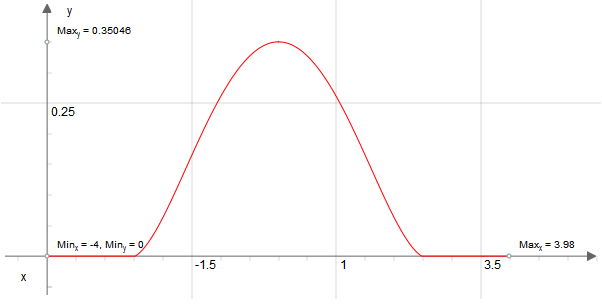
\includegraphics {MHL_BellShapedKernelExp_Graph.png}
   \caption{График функции} 
   \label{img:MHL_BellShapedKernelExp_Graph}  
 \end{figure}



\begin{lstlisting}[label=code_use_MHL_BellShapedKernelExp,caption=Пример использования]
        double z=MHL_RandomUniform(-5,5);

        //Вызов функции
        double f=MHL_BellShapedKernelExp(z);

        //Используем полученный результат
        MHL_ShowNumber(z,"Значение параметра","z");
        //Значение параметра:
        //z=0.721436
        MHL_ShowNumber(f,"Значение колоколообразного экспоненциального ядра","f");
        //Значение колоколообразного экспоненциального ядра:
        //f=0.302588
\end{lstlisting}

\subsubsection{MHL\_BellShapedKernelParabola}\label{MHL_BellShapedKernelParabola}

Колоколообразное параболическое ядро.


\begin{lstlisting}[label=code_syntax_MHL_BellShapedKernelParabola,caption=Синтаксис]
double MHL_BellShapedKernelParabola(double z);
\end{lstlisting}

\textbf{Входные параметры:}
 
z --- входная переменная.

\textbf{Возвращаемое значение:}
 
Значение функции в точке.

\textbf{Формула:}
\begin{equation*}
f\left(z \right)=\left\lbrace \begin{aligned} 0.335-0.067z^2,& \text{ если } z^2\leq 5 ; \\ 0,& \text{ иначе}. \end{aligned}\right.
\end{equation*}

 \begin{figure} [h] 
   \center
   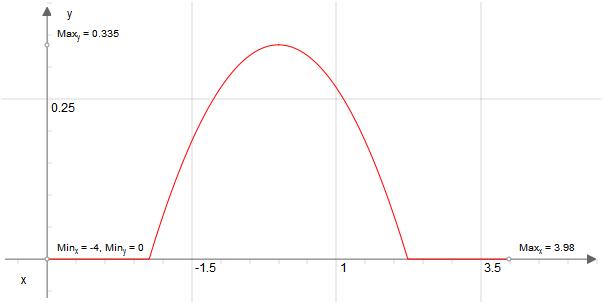
\includegraphics {MHL_BellShapedKernelParabola_Graph.png}
   \caption{График функции} 
   \label{img:MHL_BellShapedKernelParabola_Graph}  
 \end{figure}



\begin{lstlisting}[label=code_use_MHL_BellShapedKernelParabola,caption=Пример использования]
        double z=MHL_RandomUniform(-5,5);

        //Вызов функции
        double f=MHL_BellShapedKernelParabola(z);

        //Используем полученный результат
        MHL_ShowNumber(z,"Значение параметра","z");
        //Значение параметра:
        //z=0.33905
        MHL_ShowNumber(f,"Значение колоколообразного параболического ядра","f");
        //Значение колоколообразного параболического ядра:
        //f=0.327298
\end{lstlisting}

\subsubsection{MHL\_BellShapedKernelRectangle}\label{MHL_BellShapedKernelRectangle}

Колоколообразное прямоугольное ядро.


\begin{lstlisting}[label=code_syntax_MHL_BellShapedKernelRectangle,caption=Синтаксис]
double MHL_BellShapedKernelRectangle(double z);
\end{lstlisting}

\textbf{Входные параметры:}
 
z --- входная переменная.

\textbf{Возвращаемое значение:}
 
Значение функции в точке.

\textbf{Формула:}
\begin{equation*}
f\left(z \right)=\left\lbrace \begin{aligned} 0.5,& \text{ если } \left|z\right| \leq 1 ; \\ 0,& \text{ иначе}. \end{aligned}\right.
\end{equation*}

 \begin{figure} [h] 
   \center
   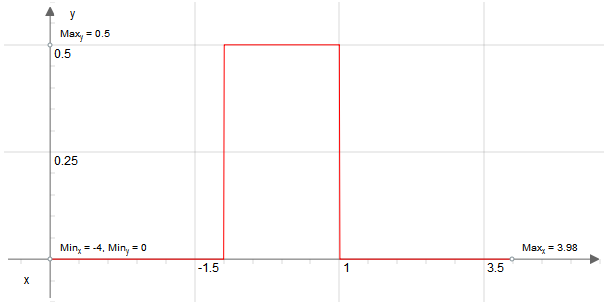
\includegraphics {MHL_BellShapedKernelRectangle_Graph.png}
   \caption{График функции} 
   \label{img:MHL_BellShapedKernelRectangle_Graph}  
 \end{figure}


\begin{lstlisting}[label=code_use_MHL_BellShapedKernelRectangle,caption=Пример использования]
        double z=MHL_RandomUniform(-5,5);

        //Вызов функции
        double f=MHL_BellShapedKernelRectangle(z);

        //Используем полученный результат
        MHL_ShowNumber(z,"Значение параметра","z");
        //Значение параметра:
        //z=0.669556
        MHL_ShowNumber(f,"Значение колоколообразного прямоугольного ядра","f");
        //Значение колоколообразного прямоугольного ядра:
        //f=0.5
\end{lstlisting}

\subsubsection{MHL\_BellShapedKernelTriangle}\label{MHL_BellShapedKernelTriangle}

Колоколообразное треугольное ядро.


\begin{lstlisting}[label=code_syntax_MHL_BellShapedKernelTriangle,caption=Синтаксис]
double MHL_BellShapedKernelTriangle(double z);
\end{lstlisting}

\textbf{Входные параметры:}
 
z --- входная переменная.

\textbf{Возвращаемое значение:}
 
Значение функции в точке.

\textbf{Формула:}
\begin{equation*}
f\left(z \right)=\left\lbrace \begin{aligned} 1-z,& \text{ если } \left| z\right| \leq 1 ; \\ 0,& \text{ иначе}. \end{aligned}\right.
\end{equation*}

 \begin{figure} [h] 
   \center
   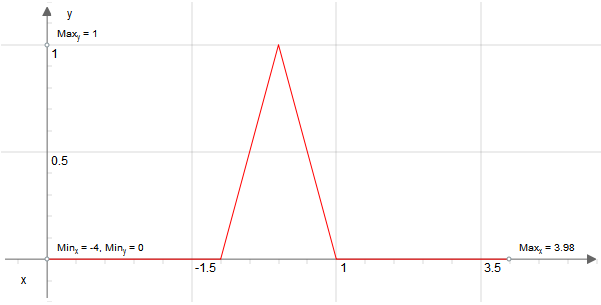
\includegraphics {MHL_BellShapedKernelTriangle_Graph.png}
   \caption{График функции} 
   \label{img:MHL_BellShapedKernelTriangle_Graph}  
 \end{figure}


\begin{lstlisting}[label=code_use_MHL_BellShapedKernelTriangle,caption=Пример использования]
        double z=MHL_RandomUniform(-5,5);

        //Вызов функции
        double f=MHL_BellShapedKernelTriangle(z);

        //Используем полученный результат
        MHL_ShowNumber(z,"Значение параметра","z");
        //Значение параметра:
        //z=0.362854
        MHL_ShowNumber(f,"Значение колоколообразного треугольного ядра","f");
        //Значение колоколообразного треугольного ядра:
        //f=0.637146
\end{lstlisting}

\subsubsection{MHL\_DerivativeOfBellShapedKernelExp}\label{MHL_DerivativeOfBellShapedKernelExp}

Производная колоколообразного экспоненциального ядра.


\begin{lstlisting}[label=code_syntax_MHL_DerivativeOfBellShapedKernelExp,caption=Синтаксис]
double MHL_DerivativeOfBellShapedKernelExp(double z);
\end{lstlisting}

\textbf{Входные параметры:}
 
z --- входная переменная.

\textbf{Возвращаемое значение:}
 
Значение функции в точке.

\textbf{Формула:}
\begin{equation*}
f\left(z \right)=\left\lbrace \begin{aligned} 0.05968\left( e^z+e^{-z}\right)-0.308586 z,& \text{ если } \left| z\right|\leq 2.47638181818 ; \\ 0,& \text{ иначе}. \end{aligned}\right.
\end{equation*}

 \begin{figure} [h] 
   \center
   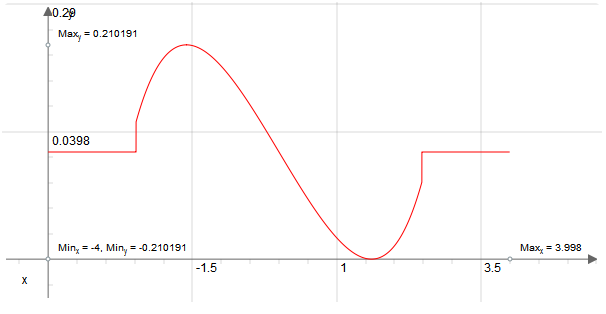
\includegraphics {MHL_DerivativeOfBellShapedKernelExp_Graph.png}
   \caption{График функции} 
   \label{img:MHL_DerivativeOfBellShapedKernelExp_Graph}  
 \end{figure}


\begin{lstlisting}[label=code_use_MHL_DerivativeOfBellShapedKernelExp,caption=Пример использования]
        double z=MHL_RandomUniform(-4,4);

        //Вызов функции
        double f=MHL_DerivativeOfBellShapedKernelExp(z);

        //Используем полученный результат
        MHL_ShowNumber(z,"Значение параметра","z");
        //Значение параметра:
        //z=-1.93701
        MHL_ShowNumber(f,"Значение производной колоколообразного экспоненциального ядра","f");
        //Значение производной колоколообразного экспоненциального ядра:
        //f=0.192278
\end{lstlisting}

\subsubsection{MHL\_DerivativeOfBellShapedKernelParabola}\label{MHL_DerivativeOfBellShapedKernelParabola}

Производная колоколообразного параболического ядра.


\begin{lstlisting}[label=code_syntax_MHL_DerivativeOfBellShapedKernelParabola,caption=Синтаксис]
double MHL_DerivativeOfBellShapedKernelParabola(double z);
\end{lstlisting}

\textbf{Входные параметры:}
 
z --- входная переменная.

\textbf{Возвращаемое значение:}
 
Значение функции в точке.

\textbf{Формула:}
\begin{equation*}
f\left(z \right)=\left\lbrace \begin{aligned} -0.134z,& \text{ если } z^2\leq 5 ; \\ 0,& \text{ иначе}. \end{aligned}\right.
\end{equation*}

 \begin{figure} [h] 
   \center
   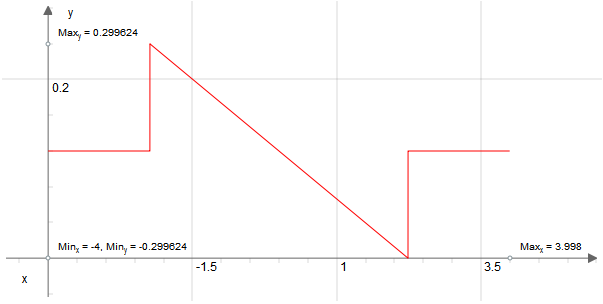
\includegraphics {MHL_DerivativeOfBellShapedKernelParabola_Graph.png}
   \caption{График функции} 
   \label{img:MHL_DerivativeOfBellShapedKernelParabola_Graph}  
 \end{figure}


\begin{lstlisting}[label=code_use_MHL_DerivativeOfBellShapedKernelParabola,caption=Пример использования]
        double z=MHL_RandomUniform(-4,4);

        //Вызов функции
        double f=MHL_DerivativeOfBellShapedKernelParabola(z);

        //Используем полученный результат
        MHL_ShowNumber(z,"Значение параметра","z");
        //Значение параметра:
        //z=1.28394
        MHL_ShowNumber(f,"Значение производной колоколообразного параболического ядра","f");
        //Значение производной колоколообразного параболического ядра:
        //f=-0.172047
\end{lstlisting}

\subsubsection{MHL\_DerivativeOfBellShapedKernelRectangle}\label{MHL_DerivativeOfBellShapedKernelRectangle}

Производная колоколообразного прямоугольного ядра.


\begin{lstlisting}[label=code_syntax_MHL_DerivativeOfBellShapedKernelRectangle,caption=Синтаксис]
double MHL_DerivativeOfBellShapedKernelRectangle(double z);
\end{lstlisting}

\textbf{Входные параметры:}
 
z --- входная переменная.

\textbf{Возвращаемое значение:}
 
Значение функции в точке.

\textbf{Формула:}
\begin{equation*}
f\left(z \right)=\left\lbrace \begin{aligned} -\infty,& \text{ если } z = 1 ; \\\infty,& \text{ если } z = -1 ; \\ 0,& \text{ иначе}. \end{aligned}\right.
\end{equation*}


\begin{lstlisting}[label=code_use_MHL_DerivativeOfBellShapedKernelRectangle,caption=Пример использования]
        double z=MHL_RandomUniform(-4,4);

        //Вызов функции
        double f=MHL_DerivativeOfBellShapedKernelRectangle(z);

        //Используем полученный результат
        MHL_ShowNumber(z,"Значение параметра","z");
        //Значение параметра:
        //z=3.146
        MHL_ShowNumber(f,"Значение производной колоколообразного прямоугольного ядра","f");
        //Значение производной колоколообразного прямоугольного ядра:
        //f=0
\end{lstlisting}

\subsubsection{MHL\_DerivativeOfBellShapedKernelTriangle}\label{MHL_DerivativeOfBellShapedKernelTriangle}

Производная колоколообразного треугольного ядра.


\begin{lstlisting}[label=code_syntax_MHL_DerivativeOfBellShapedKernelTriangle,caption=Синтаксис]
double MHL_DerivativeOfBellShapedKernelTriangle(double z);
\end{lstlisting}

\textbf{Входные параметры:}
 
z --- входная переменная.

\textbf{Возвращаемое значение:}
 
Значение функции в точке.

\textbf{Формула:}
\begin{equation*}
f\left(z \right)=\left\lbrace \begin{aligned} -1,& \text{ если } z \in \left[ 0; 1\right]   ; \\1,& \text{ если } z \in \left[ -1; 0\right) ; \\ 0,& \text{ иначе}. \end{aligned}\right.
\end{equation*}

 \begin{figure} [h] 
   \center
   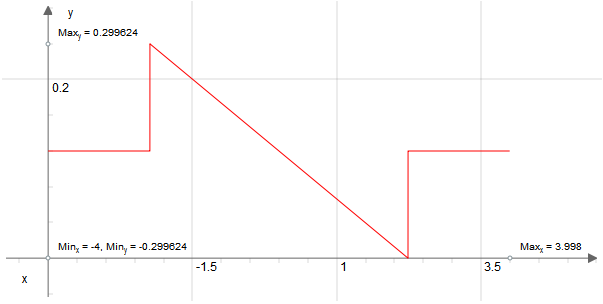
\includegraphics {MHL_DerivativeOfBellShapedKernelParabola_Graph.png}
   \caption{График функции} 
   \label{img:MHL_DerivativeOfBellShapedKernelParabola_Graph}  
 \end{figure}


\begin{lstlisting}[label=code_use_MHL_DerivativeOfBellShapedKernelTriangle,caption=Пример использования]
        double z=MHL_RandomUniform(-4,4);

        //Вызов функции
        double f=MHL_DerivativeOfBellShapedKernelTriangle(z);

        //Используем полученный результат
        MHL_ShowNumber(z,"Значение параметра","z");
        //Значение параметра:
        //z=0.365479
        MHL_ShowNumber(f,"Значение производной колоколообразного треугольного ядра","f");
        //Значение производной колоколообразного треугольного ядра:
        //f=-1
\end{lstlisting}

\subsection{Нечеткие системы}

\subsubsection{MHL\_TrapeziformFuzzyNumber}\label{MHL_TrapeziformFuzzyNumber}

Трапециевидное нечеткое число. Точнее его функция принадлежности.


\begin{lstlisting}[label=code_syntax_MHL_TrapeziformFuzzyNumber,caption=Синтаксис]
double MHL_TrapeziformFuzzyNumber(double x,double a,double b,double c,double d);
\end{lstlisting}

\textbf{Входные параметры:}
  
x --- действительное число, для которого считаем функцию принадлежности.
 
a --- левая крайняя граница;
 
b --- начало устойчивой области;
 
с --- конец устойчивой области;
 
d --- правая крайняя граница.

\textbf{Возвращаемое значение:}
 
Значение функции принадлежности.

\textbf{Формула:}
\begin{equation*}
f\left(x \right)=\left\lbrace \begin{aligned}  0,& \text{ если } x < a   ; \\\dfrac{x-a}{b-a},& \text{ если } z \in \left[ a; b\right)   ; \\1,& \text{ если } z \in \left[ b; c\right] ; \\\dfrac{d-x}{d-c},& \text{ если } z \in \left( c; d\right]   ; \\ 0,& \text{ если } z >d. \end{aligned}\right.
\end{equation*}

 \begin{figure} [h] 
   \center
   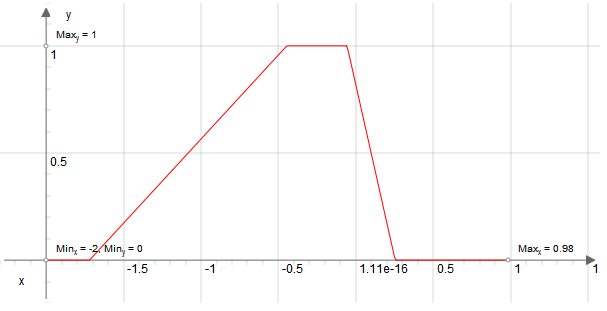
\includegraphics {MHL_TrapeziformFuzzyNumber_Graph.png}
   \caption{График функции} 
   \label{img:MHL_TrapeziformFuzzyNumber_Graph}  
 \end{figure}



\begin{lstlisting}[label=code_use_MHL_TrapeziformFuzzyNumber,caption=Пример использования]
        double a=MHL_RandomUniform(-4,4);
        double b=a+MHL_RandomUniform(0,2);
        double c=b+MHL_RandomUniform(0,2);
        double d=c+MHL_RandomUniform(0,2);

        double x=MHL_RandomUniform(a-1,d+1);

        //Вызов функции
        double f=MHL_TrapeziformFuzzyNumber (x,a,b,c,d);

        //Используем полученный результат
        MHL_ShowNumber(x,"Значение параметра","x");
        //Значение параметра:
        //x=-0.932339
        MHL_ShowNumber(a,"Значение первого параметра трапецевидного нечеткого числа","a");
        //Значение первого параметра трапецевидного нечеткого числа:
        //a=-1.71997
        MHL_ShowNumber(b,"Значение второго параметра трапецевидного нечеткого числа","b");
        //Значение второго параметра трапецевидного нечеткого числа:
        //b=-0.446045
        MHL_ShowNumber(c,"Значение третьего параметра трапецевидного нечеткого числа","c");
        //Значение третьего параметра трапецевидного нечеткого числа:
        //c=-0.0568848
        MHL_ShowNumber(d,"Значение последнего параметра трапецевидного нечеткого числа","d");
        //Значение последнего параметра трапецевидного нечеткого числа:
        //d=0.253784
        MHL_ShowNumber(f,"Значение функция принадлежности трапециевидного нечеткого числа","f");
        //Значение функция принадлежности трапециевидного нечеткого числа:
        //f=0.618271
\end{lstlisting}

\subsection{Оптимизация}

\subsubsection{MHL\_BinaryMonteCarloAlgorithm}\label{MHL_BinaryMonteCarloAlgorithm}

Метод Монте-Карло (Monte-Carlo). Простейший метод оптимизации на бинарных строках. В простонародье его называют <<методом научного тыка>>. Алгоритм оптимизации. Ищет максимум функции пригодности FitnessFunction.


\begin{lstlisting}[label=code_syntax_MHL_BinaryMonteCarloAlgorithm,caption=Синтаксис]
int MHL_BinaryMonteCarloAlgorithm(int *Parameters, double (*FitnessFunction)(int*,int), int *VMHL_ResultVector, double *VMHL_Result);
\end{lstlisting}

\textbf{Входные параметры:}

 Parameters:
 
 \begin{itemize}
 \item [0] --- длина бинарной строки (определается задачей оптимизации, что мы решаем);
 \item [1] --- число вычислений функции пригодности (CountOfFitness);
 \end{itemize}
  
 FitnessFunction --- указатель на функцию пригодности (не целевая функция, а именно функция пригодности);
 
 VMHL\_ResultVector --- найденное решение (бинарный вектор);
 
 VMHL\_Result --- значение функции в точке, определенной вектором VMHL\_ResultVector.

\textbf{Возвращаемое значение:}
 
 1 --- завершил работу без ошибок. Всё хорошо.
 
 0 --- возникли при работе ошибки. Скорее всего в этом случае в VMHL\_ResultVector и в VMHL\_Result не содержится решение задачи.
 
\textbf{Пример значений рабочего вектора Parameters:}

 Parameters[0]=20;
 
 Parameters[1]=100*100;
 
 \textbf{Принцип работы:}
 
 Принцип прост. Берутся случайно CountOfFitness решений независимо друг от друга. Выбирается лучшее. Всё.
 
 \textbf{ О функции:}
 
 В простонародье алгоритм называют <<методом научного тыка>>.
 
Алгоритм оптимизации. Ищет максимум функции пригодности FitnessFunction.

Решением является бинарная строка, то есть вектор, состоящий из 0 и 1.

\begin{lstlisting}[caption=Оптимизируемая функция]
double Func(int *x,int VMHL_N)
{
//Сумма всех элементов массива
return TMHL_SumVector(x,VMHL_N);
}
//---------------------------------------------------------------------------
\end{lstlisting}


\begin{lstlisting}[label=code_use_MHL_BinaryMonteCarloAlgorithm,caption=Пример использования]
        int LengthBinarString=50;//Длина хромосомы
        int CountOfFitness=50*50;//Число вычислений функции пригодности

        int *ParametersOfBinaryMonteCarloAlgorithm;
        ParametersOfBinaryMonteCarloAlgorithm=new int[2];
        ParametersOfBinaryMonteCarloAlgorithm[0]=LengthBinarString;//Длина хромосомы
        ParametersOfBinaryMonteCarloAlgorithm[1]=CountOfFitness;//Число вычислений целевой функции

        int *Decision;//бинарное решение
        Decision=new int[LengthBinarString];
        double ValueOfFitnessFunction;//значение функции пригодности в точке Decision
        int VMHL_Success=0;//Успешен ли будет запуск cГА

        //Запуск алгоритма
        VMHL_Success=MHL_BinaryMonteCarloAlgorithm (ParametersOfBinaryMonteCarloAlgorithm,Func, Decision, &ValueOfFitnessFunction);

        //Используем полученный результат
        MHL_ShowNumber(VMHL_Success,"Как прошел запуск","VMHL_Success");
        //Как прошел запуск:
        //VMHL_Success=1

        if (VMHL_Success==1)
         {
         MHL_ShowVectorT(Decision,LengthBinarString,"Найденное решение","Decision");
         //Найденное решение:
         //Decision =
         //1	0	1	1	1	1	1	0	1	1	1	1	1	1	1	0	0	1	0	0	1	1	1	1	1	0	1	1	0	1	1	0	1	1	1	1	0	0	1	1	1	1	0	1	1	1	0	1	1	1

         MHL_ShowNumber(ValueOfFitnessFunction,"Значение функции пригодности","ValueOfFitnessFunction");
         // Значение функции пригодности:
         //ValueOfFitnessFunction=37
         }
        delete [] ParametersOfBinaryMonteCarloAlgorithm;
        delete [] Decision;
\end{lstlisting}

\subsection{Перевод единиц измерений}

\subsubsection{MHL\_DegToRad}\label{MHL_DegToRad}

Функция переводит угол из градусной меры в радианную.


\begin{lstlisting}[label=code_syntax_MHL_DegToRad,caption=Синтаксис]
double MHL_DegToRad(double VMHL_X);
\end{lstlisting}

\textbf{Входные параметры:}

 VMHL\_X --- градусная мера угла.

\textbf{Возвращаемое значение:}
Радианная мера угла.


\begin{lstlisting}[label=code_use_MHL_DegToRad,caption=Пример использования]
        double Rad;
        double Deg=90;//Угол в градусах

        //Вызов функции
        Rad=MHL_DegToRad(Deg);

        //Используем полученный результат
        MHL_ShowNumber(Rad,"Угол "+MHL_NumberToText(Deg)+" градусов","равен в радианах");
        //Угол 90 градусов:
        //равен в радианах=1.5708
\end{lstlisting}

\subsubsection{MHL\_RadToDeg}\label{MHL_RadToDeg}

Функция переводит угол из радианной меры в градусную.


\begin{lstlisting}[label=code_syntax_MHL_RadToDeg,caption=Синтаксис]
double MHL_RadToDeg(double VMHL_X);
\end{lstlisting}

\textbf{Входные параметры:}

 VMHL\_X --- радианная мера угла.

\textbf{Возвращаемое значение:}
Градусная мера угла.


\begin{lstlisting}[label=code_use_MHL_RadToDeg,caption=Пример использования]
        double Deg;
        double Rad=MHL_PI;//Угол в радианах

        //Вызов функции
        Deg=MHL_RadToDeg(Rad);

        //Используем полученный результат
        MHL_ShowNumber(Deg,"Угол "+MHL_NumberToText(Rad)+" радиан","равен в градусах");
        //Угол 3.14159 радиан:
        //равен в градусах=180
\end{lstlisting}

\subsection{Случайные объекты}

\subsubsection{MHL\_BitNumber}\label{MHL_BitNumber}

Функция с вероятностью P (или 0.5 в переопределенной функции) возвращает 1. В противном случае возвращает 0.


\begin{lstlisting}[label=code_syntax_MHL_BitNumber,caption=Синтаксис]
int MHL_BitNumber(double P);
int MHL_BitNumber();
\end{lstlisting}

Есть две функции с разным набором аргументов.

Для первой функции:

\textbf{Входные параметры:}

 P --- вероятность появления 1.

\textbf{Возвращаемое значение:}
1 или 0.

Для второй функции:

\textbf{Входные параметры:}

 Отсутствуют.

\textbf{Возвращаемое значение:}
1 или 0.


\begin{lstlisting}[label=code_use_MHL_BitNumber,caption=Пример использования]
        int x;
        double P=0.8;//Угол в радианах

        //Вызов функции
        x=MHL_BitNumber(P);

        //Используем полученный результат
        MHL_ShowNumber(x,"Из 0 и 1 с вероятностью "+MHL_NumberToText(P),"выбрано");

        //Вызов функции
        x=MHL_BitNumber();

        //Используем полученный результат
        MHL_ShowNumber(x,"Из 0 и 1 с вероятностью 0.5","выбрано");
\end{lstlisting}

\subsubsection{MHL\_RandomRealMatrix}\label{MHL_RandomRealMatrix}

Функция заполняет матрицу случайными вещественными числами из определенного интервала [Left;Right].


\begin{lstlisting}[label=code_syntax_MHL_RandomRealMatrix,caption=Синтаксис]
void MHL_RandomRealMatrix(double **VMHL_ResultMatrix, double Left, double Right, int VMHL_N, int VMHL_M);
\end{lstlisting}

\textbf{Входные параметры:}

 VMHL\_ResultMatrix --- указатель на матрицу;
 
 Left --- левая граница интервала;
 
 Right --- правая граница интервала;
 
 VMHL\_N --- размер массива (число строк);
 
 VMHL\_M --- размер массива (число столбцов).

\textbf{Возвращаемое значение:}
Отсутствует.


\begin{lstlisting}[label=code_use_MHL_RandomRealMatrix,caption=Пример использования]
        int i;
        int VMHL_N=3;//Размер массива (число строк)
        int VMHL_M=3;//Размер массива (число столбцов)
        double **a;
        a=new double*[VMHL_N];
        for (i=0;i<VMHL_N;i++) a[i]=new double[VMHL_M];

        double Left=-3;//левая граница интервала;
        double Right=3;//правая граница интервала;

        //Вызов функции
        MHL_RandomRealMatrix(a,Left,Right,VMHL_N,VMHL_M);

        //Используем полученный результат
        MHL_ShowMatrix (a,VMHL_N,VMHL_M,"Случайная матрица", "a");
        //Случайная матрица:
        //a =
        //1.97571	0.862793	-0.357422
        //-2.62701	-0.202515	-2.79932
        //1.38794	1.35535	-2.29449

        for (i=0;i<VMHL_N;i++) delete [] a[i];
        delete [] a;
\end{lstlisting}

\subsubsection{MHL\_RandomRealMatrixInCols}\label{MHL_RandomRealMatrixInCols}

Функция заполняет матрицу случайными вещественными числами из определенного интервала. При этом элементы каждого столбца изменяются в своих пределах.


\begin{lstlisting}[label=code_syntax_MHL_RandomRealMatrixInCols,caption=Синтаксис]
void MHL_RandomRealMatrixInCols(double **VMHL_ResultMatrix, double *Left, double *Right, int VMHL_N, int VMHL_M);
\end{lstlisting}

\textbf{Входные параметры:}

 VMHL\_ResultMatrix --- указатель на матрицу;
 
 Left --- левые границы интервала изменения элементов столбца (размер VMHL\_M);
 
 Right --- правые границы интервала изменения элементов столбца (размер VMHL\_M);
 
 VMHL\_N --- размер массива (число строк);
 
 VMHL\_M --- размер массива (число столбцов).

\textbf{Возвращаемое значение:}
Отсутствует.


\begin{lstlisting}[label=code_use_MHL_RandomRealMatrixInCols,caption=Пример использования]
        int i;
        int VMHL_N=3;//Размер массива (число строк)
        int VMHL_M=3;//Размер массива (число столбцов)
        double **a;
        a=new double*[VMHL_N];
        for (i=0;i<VMHL_N;i++) a[i]=new double[VMHL_M];
        double *Left;
        Left=new double[VMHL_M];
        double *Right;
        Right=new double[VMHL_M];

        Left[0]=-5;//левая границы интервала изменения 1 столбца
        Right[0]=-4; //правая граница интервала изменения 1 столбца

        Left[1]=0;//левая границы интервала изменения 2 столбца
        Right[1]=3; //правая граница интервала изменения 2 столбца

        Left[2]=100;//левая границы интервала изменения 3 столбца
        Right[2]=200; //правая граница интервала изменения 3 столбца

        //Вызов функции
        MHL_RandomRealMatrixInCols(a,Left,Right,VMHL_N,VMHL_M);

        //Используем полученный результат
        MHL_ShowMatrix (a,VMHL_N,VMHL_M,"Случайная матрица", "a");
        //Случайная матрица:
        //a =
        //-4.20267	2.20367	148.468
        //-4.42432	2.09418	138.654
        //-4.07089	1.95831	140.198

        for (i=0;i<VMHL_N;i++) delete [] a[i];
        delete [] a;
        delete [] Left;
        delete [] Right;
\end{lstlisting}

\subsubsection{MHL\_RandomRealMatrixInElements}\label{MHL_RandomRealMatrixInElements}

Функция заполняет матрицу случайными вещественными числами из определенного интервала. При этом каждый элемент изменяется в своих пределах.


\begin{lstlisting}[label=code_syntax_MHL_RandomRealMatrixInElements,caption=Синтаксис]
void MHL_RandomRealMatrixInElements(double **VMHL_ResultMatrix, double **Left, double **Right, int VMHL_N, int VMHL_M);
\end{lstlisting}

\textbf{Входные параметры:}

 VMHL\_ResultMatrix --- указатель на матрицу;
 
Left --- левые границы интервала изменения каждого элемента (размер VMHL\_N x VMHL\_M);

 Right --- правые границы интервала изменения каждого элемента (размер VMHL\_N x VMHL\_M);
 
 VMHL\_N --- размер массива (число строк);
 
 VMHL\_M --- размер массива (число столбцов).

\textbf{Возвращаемое значение:}
Отсутствует.


\begin{lstlisting}[label=code_use_MHL_RandomRealMatrixInElements,caption=Пример использования]
        int i,j;
        int VMHL_N=3;//Размер массива (число строк)
        int VMHL_M=3;//Размер массива (число столбцов)
        double **a;
        a=new double*[VMHL_N];
        for (i=0;i<VMHL_N;i++) a[i]=new double[VMHL_M];
        double **Left;
        Left=new double*[VMHL_N];
        for (i=0;i<VMHL_N;i++) Left[i]=new double[VMHL_M];
        double **Right;
        Right=new double*[VMHL_N];
        for (i=0;i<VMHL_N;i++) Right[i]=new double[VMHL_M];

        //Возьмем для примера границы интервала равными около номера ячейки в матрице
        for (i=0;i<VMHL_N;i++)
         for (j=0;j<VMHL_M;j++)
          {
          Left[i][j]=i*VMHL_N+j-0.1;
          Right[i][j]=Left[i][j]+0.2;
          }

        //Вызов функции
        MHL_RandomRealMatrixInElements(a,Left,Right,VMHL_N,VMHL_M);

        //Используем полученный результат

        MHL_ShowMatrix (Left,VMHL_N,VMHL_M,"Матрица левых границ", "Left");
        // Матрица левых границ:
        //Left =
        //-0.1	0.9	1.9
        //2.9	3.9	4.9
        //5.9	6.9	7.9

        MHL_ShowMatrix (Right,VMHL_N,VMHL_M,"Матрица правых границ", "Right");
        // Матрица правых границ:
        //Right =
        //0.1	1.1	2.1
        //3.1	4.1	5.1
        //6.1	7.1	8.1

        MHL_ShowMatrix (a,VMHL_N,VMHL_M,"Случайная матрица", "a");
        // Случайная матрица:
        //a =
        //0.0829529	1.04504	1.9892
        //2.90126	3.92388	4.90221
        //5.96102	6.90623	8.09661

        for (i=0;i<VMHL_N;i++) delete [] a[i];
        delete [] a;
        for (i=0;i<VMHL_N;i++) delete [] Left[i];
        delete [] Left;
        for (i=0;i<VMHL_N;i++) delete [] Right[i];
        delete [] Right;
\end{lstlisting}

\subsubsection{MHL\_RandomRealMatrixInRows}\label{MHL_RandomRealMatrixInRows}

Функция заполняет матрицу случайными вещественными числами из определенного интервала. При этом элементы каждой строки изменяются в своих пределах.


\begin{lstlisting}[label=code_syntax_MHL_RandomRealMatrixInRows,caption=Синтаксис]
void MHL_RandomRealMatrixInRows(double **VMHL_ResultMatrix, double *Left, double *Right, int VMHL_N, int VMHL_M);
\end{lstlisting}

\textbf{Входные параметры:}

 VMHL\_ResultMatrix --- указатель на матрицу;
 
 Left --- левые границы интервала изменения элементов строки (размер VMHL\_N);
 
 Right --- правые границы интервала изменения элементов строки (размер VMHL\_N);
 
 VMHL\_N --- размер массива (число строк);
 
 VMHL\_M --- размер массива (число столбцов).

\textbf{Возвращаемое значение:}
Отсутствует.


\begin{lstlisting}[label=code_use_MHL_RandomRealMatrixInRows,caption=Пример использования]
        int i;
        int VMHL_N=3;//Размер массива (число строк)
        int VMHL_M=3;//Размер массива (число столбцов)
        double **a;
        a=new double*[VMHL_N];
        for (i=0;i<VMHL_N;i++) a[i]=new double[VMHL_M];
        double *Left;
        Left=new double[VMHL_N];
        double *Right;
        Right=new double[VMHL_N];

        Left[0]=-5;//левая границы интервала изменения 1 строки
        Right[0]=-4; //правая граница интервала изменения 1 строки

        Left[1]=0;//левая границы интервала изменения 2 строки
        Right[1]=3; //правая граница интервала изменения 2 строки

        Left[2]=100;//левая границы интервала изменения 3 строки
        Right[2]=200; //правая граница интервала изменения 3 строки

        //Вызов функции
        MHL_RandomRealMatrixInRows(a,Left,Right,VMHL_N,VMHL_M);

        //Используем полученный результат

        MHL_ShowMatrix (a,VMHL_N,VMHL_M,"Случайная матрица", "a");
        // Случайная матрица:
        //a =
        //-4.98376	-4.64868	-4.38959
        //1.14386	2.70071	2.76151
        //141.309	192.12	100.122

        for (i=0;i<VMHL_N;i++) delete [] a[i];
        delete [] a;
        delete [] Left;
        delete [] Right;
\end{lstlisting}

\subsubsection{MHL\_RandomRealVector}\label{MHL_RandomRealVector}

Функция заполняет массив случайными вещественными числами из определенного интервала [Left;Right].


\begin{lstlisting}[label=code_syntax_MHL_RandomRealVector,caption=Синтаксис]
void MHL_RandomRealVector(double *VMHL_ResultVector, double Left, double Right, int VMHL_N);
\end{lstlisting}

\textbf{Входные параметры:}

 VMHL\_ResultVector --- указатель на массив;
 
 Left --- левая граница интервала;
 
 Right --- правая граница интервала;
 
 VMHL\_N --- размер массива.

\textbf{Возвращаемое значение:}
Отсутствует.


\begin{lstlisting}[label=code_use_MHL_RandomRealVector,caption=Пример использования]
        int VMHL_N=10;//Размер массива
        double *a;
        a=new double[VMHL_N];

        double Left=-3;
        double Right=3;

        //Вызов функции
        MHL_RandomRealVector(a,Left,Right,VMHL_N);

        //Используем полученный результат
        MHL_ShowVector (a,VMHL_N,"Массив", "a");
        // Массив:
        //a =
        //1.73822
        //-0.406311
        //-2.7572
        //-0.351013
        //0.367493
        //1.40991
        //0.662476
        //-1.15576
        //-1.75781
        //-2.06927

        delete [] a;
\end{lstlisting}

\subsubsection{MHL\_RandomRealVectorInElements}\label{MHL_RandomRealVectorInElements}

Функция заполняет массив случайными вещественными числами из определенного интервала, где на каждую координату свои границы изменения.


\begin{lstlisting}[label=code_syntax_MHL_RandomRealVectorInElements,caption=Синтаксис]
void MHL_RandomRealVectorInElements(double *VMHL_ResultVector, double *Left, double *Right, int VMHL_N);
\end{lstlisting}

\textbf{Входные параметры:}

 VMHL\_ResultVector --- указатель на массив;
 
 Left --- левые границы интервалов (размер VMHL\_N);
 
 Right --- правые границы интервалов (размер VMHL\_N)
 
 VMHL\_N --- размер массива.

\textbf{Возвращаемое значение:}
Отсутствует.


\begin{lstlisting}[label=code_use_MHL_RandomRealVectorInElements,caption=Пример использования]
        int VMHL_N=2;//Размер массива
        double *a;
        a=new double[VMHL_N];

        double *Left;
        Left=new double[VMHL_N];
        Left[0]=-3;//Левая граница изменения первого элемента массива
        Left[1]=5;//Левая граница изменения второго элемента массива

        double *Right;
        Right=new double[VMHL_N];
        Right[0]=3;//Правая граница изменения первого элемента массива
        Right[1]=10;//Правая граница изменения второго элемента массива

        //Вызов функции
        MHL_RandomRealVectorInElements(a,Left,Right,VMHL_N);

        //Используем полученный результат

        MHL_ShowVector (Left,VMHL_N,"Массив левых границ", "Left");
        // Массив левых границ:
        //Left =
        //-3
        //5

        MHL_ShowVector (Right,VMHL_N,"Массив правых границ", "Right");
        // Массив правых границ:
        //Right =
        //3
        //10

        MHL_ShowVector (a,VMHL_N,"Случайных массив", "a");
        // Случайных массив:
        //a =
        //1.32111
        //6.5625

        delete [] a;
        delete [] Left;
        delete [] Right;
\end{lstlisting}

\subsubsection{MHL\_RandomVectorOfProbability}\label{MHL_RandomVectorOfProbability}

Функция заполняет вектор случайными значениями вероятностей. Сумма всех элементов вектора равна 1.


\begin{lstlisting}[label=code_syntax_MHL_RandomVectorOfProbability,caption=Синтаксис]
void MHL_RandomVectorOfProbability(double *VMHL_ResultVector, int VMHL_N);
\end{lstlisting}

\textbf{Входные параметры:}

 VMHL\_ResultVector --- указатель на вектор вероятностей (одномерный массив);
 
 VMHL\_N --- размер массива.

\textbf{Возвращаемое значение:}
Отсутствует.


\begin{lstlisting}[label=code_use_MHL_RandomVectorOfProbability,caption=Пример использования]
        int VMHL_N=10;//Размер массива (число строк)
        double *a;
        a=new double[VMHL_N];

        //Заполним вектор случайными значениями вероятностей
        //Вызов функции
        MHL_RandomVectorOfProbability(a, VMHL_N);

        //Используем полученный результат
        MHL_ShowVector (a,VMHL_N,"Вектор вероятностей выбора", "a");
        // Вектор вероятностей выбора:
        //a =	
        //0.0662721
        //0.0681826
        //0.083972
        //0.0554142
        //0.18878
        //0.160006
        //0.0698625
        //0.0652843
        //0.127822
        //0.114404         

        MHL_ShowNumber (TMHL_SumVector(a,VMHL_N),"Его сумма", "Sum");
        // Его сумма:
        //Sum=1
\end{lstlisting}

\subsubsection{TMHL\_BernulliVector}\label{TMHL_BernulliVector}

Функция формирует случайный вектор Бернулли.


\begin{lstlisting}[label=code_syntax_TMHL_BernulliVector,caption=Синтаксис]
template <class T> void TMHL_BernulliVector(T *VMHL_ResultVector, int VMHL_N);
\end{lstlisting}

\textbf{Входные параметры:} 
 
VMHL\_ResultVector --- указатель на вектор (одномерный массив);
 
VMHL\_N --- размер массива.

\textbf{Возвращаемое значение:}

Отсутствует.


\begin{lstlisting}[label=code_use_TMHL_BernulliVector,caption=Пример использования]
        int VMHL_N=10;//Размер массива (число строк)
        double *a;
        a=new double[VMHL_N];

        //Вызов функции
        TMHL_BernulliVector(a,VMHL_N);

        //Используем полученный результат
        MHL_ShowVector (a,VMHL_N,"Случайный вектор Бернулли", "a");
		//Случайный вектор Бернулли:
        //a =
        //1
        //-1
        //1
        //1
        //-1
        //1
        //-1
        //-1
        //1
        //1
\end{lstlisting}

\subsubsection{TMHL\_RandomArrangingObjectsIntoBaskets}\label{TMHL_RandomArrangingObjectsIntoBaskets}

Функция предлагает случайный способ расставить N объектов в VMHL\_N корзин при условии, что в каждой корзине может располагаться только один предмет.


\begin{lstlisting}[label=code_syntax_TMHL_RandomArrangingObjectsIntoBaskets,caption=Синтаксис]
template <class T> void TMHL_RandomArrangingObjectsIntoBaskets(T *VMHL_ResultVector, int N, int VMHL_N);
\end{lstlisting}

\textbf{Входные параметры:} 
 
VMHL\_ResultVector --- массив, в который записывается результат;
 
N --- число предметов;
 
VMHL\_N --- размер массива (и число корзин).

\textbf{Возвращаемое значение:}

Отсутствует.


\begin{lstlisting}[label=code_use_TMHL_RandomArrangingObjectsIntoBaskets,caption=Пример использования]
        int VMHL_N=10;//Размер массива
        int *a;
        a=new int[VMHL_N];

        int N=MHL_RandomUniformInt(0,10);// Размер турнира

        //Вызов функции
        TMHL_RandomArrangingObjectsIntoBaskets(a,N,VMHL_N);

        //Используем полученный результат
        MHL_ShowNumber (N,"Число предметов", "N");
        // Число предметов:
        // N=5
        MHL_ShowVectorT (a,VMHL_N,"Случаное расположение по 10 корзинам", "a");
        // Случаное расположение по 10 корзинам:
        //a =
        //0	1	0	0	0	1	1	0	1	1

        delete [] a;
\end{lstlisting}

\subsubsection{TMHL\_RandomBinaryMatrix}\label{TMHL_RandomBinaryMatrix}

Функция заполняет матрицу случайно нулями и единицами.


\begin{lstlisting}[label=code_syntax_TMHL_RandomBinaryMatrix,caption=Синтаксис]
template <class T> void TMHL_RandomBinaryMatrix(T **VMHL_ResultMatrix,int VMHL_N,int VMHL_M);
\end{lstlisting}

\textbf{Входные параметры:}
 
VMHL\_ResultMatrix --- указатель на преобразуемый массив;
 
VMHL\_N --- размер массива VMHL\_ResultMatrix (число строк);
 
VMHL\_M --- размер массива VMHL\_ResultMatrix (число столбцов). 

\textbf{Возвращаемое значение:}

Отсутствует.


\begin{lstlisting}[label=code_use_TMHL_RandomBinaryMatrix,caption=Пример использования]
        int i;
        int VMHL_N=10;//Размер массива (число строк)
        int VMHL_M=3;//Размер массива (число столбцов)
        int **a;
        a=new int*[VMHL_N];
        for (i=0;i<VMHL_N;i++) a[i]=new int[VMHL_M];

        //Вызов функции
        TMHL_RandomBinaryMatrix(a,VMHL_N,VMHL_M);

        //Используем полученный результат
        MHL_ShowMatrix (a,VMHL_N,VMHL_M,"Случайная бинарная матрица", "a");
        //Случайная бинарная матрица:
        //a =
        //1	0	1
        //0	0	0
        //1	1	1
        //1	0	0
        //1	1	0
        //1	1	0
        //0	1	1
        //0	0	1
        //1	0	0
        //1	1	0

        for (i=0;i<VMHL_N;i++) delete [] a[i];
        delete [] a;
\end{lstlisting}

\subsubsection{TMHL\_RandomBinaryVector}\label{TMHL_RandomBinaryVector}

Функция заполняет вектор (одномерный массив) случайно нулями и единицами.


\begin{lstlisting}[label=code_syntax_TMHL_RandomBinaryVector,caption=Синтаксис]
template <class T> void TMHL_RandomBinaryVector(T *VMHL_ResultVector,int VMHL_N);
\end{lstlisting}

\textbf{Входные параметры:}
 
VMHL\_ResultVector --- указатель на преобразуемый массив;
 
VMHL\_N --- размер массива VMHL\_ResultMatrix (число строк).

\textbf{Возвращаемое значение:}

Отсутствует.


\begin{lstlisting}[label=code_use_TMHL_RandomBinaryVector,caption=Пример использования]
        int VMHL_N=10;//Размер массива (число строк)
        int *a;
        a=new int[VMHL_N];

        //Вызов функции
        TMHL_RandomBinaryVector(a,VMHL_N);

        //Используем полученный результат
        MHL_ShowVector (a,VMHL_N,"Случайный бинарный вектор", "a");
        //Случайный бинарный вектор:
        //a =
        //1
        //1
        //0
        //0
        //0
        //0
        //1
        //1
        //0
        //0

        delete [] a;
\end{lstlisting}

\subsubsection{TMHL\_RandomIntMatrix}\label{TMHL_RandomIntMatrix}

Функция заполняет матрицу случайными целыми числами из определенного интервала [n;m).


\begin{lstlisting}[label=code_syntax_TMHL_RandomIntMatrix,caption=Синтаксис]
template <class T> void TMHL_RandomIntMatrix(T **VMHL_ResultMatrix, T n, T m, int VMHL_N, int VMHL_M);
\end{lstlisting}

\textbf{Входные параметры:}
 
VMHL\_ResultMatrix --- указатель на матрицу;
 
n --- левая граница интервала;
 
m --- правая граница интервала;
 
VMHL\_N --- размер массива (число строк);
 
VMHL\_M --- размер массива (число столбцов).

\textbf{Возвращаемое значение:}

Отсутствует.


\begin{lstlisting}[label=code_use_TMHL_RandomIntMatrix,caption=Пример использования]
        int i;
        int VMHL_N=3;//Размер массива (число строк)
        int VMHL_M=3;//Размер массива (число столбцов)
        int **a;
        a=new int*[VMHL_N];
        for (i=0;i<VMHL_N;i++) a[i]=new int[VMHL_M];

        int n=-3;//левая граница интервала;
        int m=3;//правая граница интервала;

        //Вызов функции
        TMHL_RandomIntMatrix(a,n,m,VMHL_N,VMHL_M);

        //Используем полученный результат

        MHL_ShowMatrix (a,VMHL_N,VMHL_M,"Случайная матрица", "a");
        // Случайная матрица:
        //a =
        //-1	-1	2
        //2	0	1
        //-3	2	-1ss

        for (i=0;i<VMHL_N;i++) delete [] a[i];
        delete [] a;
\end{lstlisting}

\subsubsection{TMHL\_RandomIntMatrixInCols}\label{TMHL_RandomIntMatrixInCols}

Функция заполняет матрицу случайными целыми числами из определенного интервала [n;m). При этом элементы каждого столбца изменяются в своих пределах.


\begin{lstlisting}[label=code_syntax_TMHL_RandomIntMatrixInCols,caption=Синтаксис]
template <class T> void TMHL_RandomIntMatrixInCols(T **VMHL_ResultMatrix, T *n, T *m, int VMHL_N, int VMHL_M);
\end{lstlisting}

\textbf{Входные параметры:}
 
VMHL\_ResultMatrix --- указатель на матрицу;
 
n --- левые границы интервала изменения элементов столбцов (размер VMHL\_M);
 
m --- правые границы интервала изменения элементов столбцов (размер VMHL\_M);
 
VMHL\_N --- размер массива (число строк);
 
VMHL\_M --- размер массива (число столбцов).

\textbf{Возвращаемое значение:}

Отсутствует.


\begin{lstlisting}[label=code_use_TMHL_RandomIntMatrixInCols,caption=Пример использования]
        int i;
        int VMHL_N=3;//Размер массива (число строк)
        int VMHL_M=3;//Размер массива (число столбцов)
        int **a;
        a=new int*[VMHL_N];
        for (i=0;i<VMHL_N;i++) a[i]=new int[VMHL_M];
        int *n;
        n=new int[VMHL_M];
        int *m;
        m=new int[VMHL_M];

        n[0]=-50;//левая границы интервала изменения 1 столбца
        m[0]=-40; //правая граница интервала изменения 1 столбца

        n[1]=0;//левая границы интервала изменения 2 столбца
        m[1]=3; //правая граница интервала изменения 2 столбца

        n[2]=100;//левая границы интервала изменения 3 столбца
        m[2]=200; //правая граница интервала изменения 3 столбца

        //Вызов функции
        TMHL_RandomIntMatrixInCols(a,n,m,VMHL_N,VMHL_M);

        //Используем полученный результат

        MHL_ShowMatrix (a,VMHL_N,VMHL_M,"Случайная матрица", "a");
        //Случайная матрица:
        //a =
        //-47	2	142
        //-47	1	139
        //-44	0	199

        for (i=0;i<VMHL_N;i++) delete [] a[i];
        delete [] a;
        delete [] n;
        delete [] m;
\end{lstlisting}

\subsubsection{TMHL\_RandomIntMatrixInElements}\label{TMHL_RandomIntMatrixInElements}

Функция заполняет матрицу случайными целыми числами из определенного интервала [n;m). При этом каждый элемент изменяется в своих пределах.


\begin{lstlisting}[label=code_syntax_TMHL_RandomIntMatrixInElements,caption=Синтаксис]
template <class T> void TMHL_RandomIntMatrixInElements(T **VMHL_ResultMatrix, T **n, T **m, int VMHL_N, int VMHL_M);
\end{lstlisting}

\textbf{Входные параметры:}
 
VMHL\_ResultMatrix --- указатель на матрицу;
 
n --- левые границы интервала изменения каждого элемента (размер VMHL\_N x VMHL\_M);
 
m --- правые границы интервала изменения каждого элемента (размер VMHL\_N x VMHL\_M);
 
VMHL\_N --- размер массива (число строк);
 
VMHL\_M --- размер массива (число столбцов).

\textbf{Возвращаемое значение:}

Отсутствует.


\begin{lstlisting}[label=code_use_TMHL_RandomIntMatrixInElements,caption=Пример использования]
        int i,j;
        int VMHL_N=3;//Размер массива (число строк)
        int VMHL_M=3;//Размер массива (число столбцов)
        int **a;
        a=new int*[VMHL_N];
        for (i=0;i<VMHL_N;i++) a[i]=new int[VMHL_M];
        int **n;
        n=new int*[VMHL_N];
        for (i=0;i<VMHL_N;i++) n[i]=new int[VMHL_M];
        int **m;
        m=new int*[VMHL_N];
        for (i=0;i<VMHL_N;i++) m[i]=new int[VMHL_M];

        //Заполним границы изменения каждого элемента
        for (i=0;i<VMHL_N;i++)
         for (j=0;j<VMHL_M;j++)
          {
          n[i][j]=i*VMHL_N+j-10;
          m[i][j]=n[i][j]+20;
          }

        //Вызов функции
        TMHL_RandomIntMatrixInElements(a,n,m,VMHL_N,VMHL_M);

        //Используем полученный результат

        MHL_ShowMatrix (n,VMHL_N,VMHL_M,"Матрица левых границ", "n");
        //Матрица левых границ:
        //n =
        //-10	-9	-8
        //-7	-6	-5
        //-4	-3	-2

        MHL_ShowMatrix (m,VMHL_N,VMHL_M,"Матрица правых границ", "m");
        // Матрица правых границ:
        //m =
        //10	11	12
        //13	14	15
        //16	17	18

        MHL_ShowMatrix (a,VMHL_N,VMHL_M,"Случайная матрица", "a");
        // Случайная матрица:
        //a =
        //-4	6	-8
        //-1	1	1
        //-3	16	4

        for (i=0;i<VMHL_N;i++) delete [] a[i];
        delete [] a;
        for (i=0;i<VMHL_N;i++) delete [] n[i];
        delete [] n;
        for (i=0;i<VMHL_N;i++) delete [] m[i];
        delete [] m;
\end{lstlisting}

\subsubsection{TMHL\_RandomIntMatrixInRows}\label{TMHL_RandomIntMatrixInRows}

Функция заполняет матрицу случайными целыми числами из определенного интервала [n;m). При этом элементы каждой строки изменяются в своих пределах.


\begin{lstlisting}[label=code_syntax_TMHL_RandomIntMatrixInRows,caption=Синтаксис]
template <class T> void TMHL_RandomIntMatrixInRows(T **VMHL_ResultMatrix, T *n, T *m, int VMHL_N, int VMHL_M);
\end{lstlisting}

\textbf{Входные параметры:}
 
VMHL\_ResultMatrix --- указатель на матрицу;
 
n --- левые границы интервала изменения элементов строки (размер VMHL\_N);
 
m --- правые границы интервала изменения элементов строки (размер VMHL\_N);
 
VMHL\_N --- размер массива (число строк);
 
VMHL\_M --- размер массива (число столбцов).

\textbf{Возвращаемое значение:}

Отсутствует.


\begin{lstlisting}[label=code_use_TMHL_RandomIntMatrixInRows,caption=Пример использования]
        int i;
        int VMHL_N=3;//Размер массива (число строк)
        int VMHL_M=3;//Размер массива (число столбцов)
        int **a;
        a=new int*[VMHL_N];
        for (i=0;i<VMHL_N;i++) a[i]=new int[VMHL_M];
        int *n;
        n=new int[VMHL_N];
        int *m;
        m=new int[VMHL_N];

        n[0]=-50;//левая границы интервала изменения 1 строки
        m[0]=-40; //правая граница интервала изменения 1 строки

        n[1]=0;//левая границы интервала изменения 2 строки
        m[1]=3; //правая граница интервала изменения 2 строки

        n[2]=100;//левая границы интервала изменения 3 строки
        m[2]=200; //правая граница интервала изменения 3 строки

        //Вызов функции
        TMHL_RandomIntMatrixInRows(a,n,m,VMHL_N,VMHL_M);

        //Используем полученный результат

        MHL_ShowMatrix (a,VMHL_N,VMHL_M,"Случайная матрица", "a");
        // Случайная матрица:
        //a =
        // -42	-42	-45
        //2	2	0
        //113	102	109

        for (i=0;i<VMHL_N;i++) delete [] a[i];
        delete [] a;
        delete [] n;
        delete [] m;
\end{lstlisting}

\subsubsection{TMHL\_RandomIntVector}\label{TMHL_RandomIntVector}

Функция заполняет массив случайными целыми числами из определенного интервала [n,m).


\begin{lstlisting}[label=code_syntax_TMHL_RandomIntVector,caption=Синтаксис]
template <class T> void TMHL_RandomIntVector(T *VMHL_ResultVector, T n, T m, int VMHL_N);
\end{lstlisting}

\textbf{Входные параметры:}
 
VMHL\_ResultVector --- указатель на массив;
 
n --- левая граница интервала;
 
m --- правая граница интервала;
 
VMHL\_N --- размер массива.

\textbf{Возвращаемое значение:}

Отсутствует.


\begin{lstlisting}[label=code_use_TMHL_RandomIntVector,caption=Пример использования]
        int VMHL_N=10;//Размер массива
        int *a;
        a=new int[VMHL_N];

        int n=3;
        int m=50;

        //Вызов функции
        TMHL_RandomIntVector(a,n,m,VMHL_N);

        //Используем полученный результат

        MHL_ShowVector (a,VMHL_N,"Массив", "a");
        //Массив:
        //a =
        //6
        //23
        //40
        //19
        //39
        //37
        //48
        //46
        //31
        //42

        delete [] a;
\end{lstlisting}

\subsubsection{TMHL\_RandomIntVectorInElements}\label{TMHL_RandomIntVectorInElements}

Функция заполняет массив случайными целыми  числами из определенного интервала [n\_i,m\_i). При этом для каждого элемента массива свой интервал изменения.


\begin{lstlisting}[label=code_syntax_TMHL_RandomIntVectorInElements,caption=Синтаксис]
template <class T> void TMHL_RandomIntVectorInElements(T *VMHL_ResultVector, T *n, T *m, int VMHL_N);
\end{lstlisting}

\textbf{Входные параметры:}
 
VMHL\_ResultVector --- указатель на массив;
 
n --- указатель на массив левых границ интервала;
 
m --- указатель на массив правых границ интервала;
 
VMHL\_N --- размер массива.

\textbf{Возвращаемое значение:}

Отсутствует.


\begin{lstlisting}[label=code_use_TMHL_RandomIntVectorInElements,caption=Пример использования]
        int VMHL_N=2;//Размер массива
        int *a;
        a=new int[VMHL_N];

        int *n;
        n=new int[VMHL_N];
        n[0]=3;//Левая граница изменения первого элемента массива
        n[1]=-90;//Левая граница изменения второго элемента массива

        int *m;
        m=new int[VMHL_N];
        m[0]=40;//Правая граница изменения первого элемента массива
        m[1]=-10;//Правая граница изменения второго элемента массива

        //Вызов функции
        TMHL_RandomIntVectorInElements(a,n,m,VMHL_N);

        //Используем полученный результат

        MHL_ShowVector (n,VMHL_N,"Массив левых границ", "n");
        //Массив левых границ:
        //n =
        //3
        //-90

        MHL_ShowVector (m,VMHL_N,"Массив правых границ", "m");
        // Массив правых границ:
        //m =
        //40
        //-10

        MHL_ShowVector (a,VMHL_N,"Случайных массив", "a");
        // Случайных массив:
        //a =
        //31
        //-52

        delete [] a;
        delete [] n;
        delete [] m;
\end{lstlisting}

\subsubsection{TMHL\_RandomMatrixOfPermutation}\label{TMHL_RandomMatrixOfPermutation}

Функция создает случайный массив строк-перестановок чисел от 1 до VMHL\_M.


\begin{lstlisting}[label=code_syntax_TMHL_RandomMatrixOfPermutation,caption=Синтаксис]
template <class T> void TMHL_RandomMatrixOfPermutation(T **VMHL_ResultMatrix, int VMHL_N, int VMHL_M);
\end{lstlisting}

\textbf{Входные параметры:}
 
 VMHL\_ResultMatrix --- указатель на матрицу;
 
 VMHL\_N --- размер массива (число строк);
 
 VMHL\_M --- размер массива (число столбцов).

\textbf{Возвращаемое значение:} 

Отсутствует.

\textbf{О функции:}

Строка-перестановка --- это массив натуральных чисел от 1 до VMHL\_M расположенных в произвольном порядке. Например, если VMHL\_M=10, то строкой-перестановкой будет массив 7 5 2 4 6 8 1 10 3 9. Эти строки используются в комбинаторной оптимизации.



\begin{lstlisting}[label=code_use_TMHL_RandomMatrixOfPermutation,caption=Пример использования]
        int i;
        int VMHL_N=10;//Размер массива (число строк)
        int VMHL_M=5;//Размер массива (число строк)
        int **a;
        a=new int*[VMHL_N];
        for (i=0;i<VMHL_N;i++) a[i]=new int[VMHL_M];

        //Вызов функции
        TMHL_RandomMatrixOfPermutation(a,VMHL_N,VMHL_M);

        //Используем полученный результат
        MHL_ShowMatrix (a,VMHL_N,VMHL_M,"Матрица строк-перестановок", "a");
        //Матрица строк-перестановок:
        //a =
        //3	2	1	4	5
        //4	1	3	2	5
        //5	2	3	4	1
        //5	3	4	2	1
        //5	4	2	1	3
        //1	4	3	5	2
        //5	4	1	3	2
        //1	4	2	5	3
        //3	1	2	4	5
        //5	3	4	2	1

        for (i=0;i<VMHL_N;i++) delete [] a[i];
        delete [] a;
\end{lstlisting}

\subsubsection{TMHL\_RandomVectorOfPermutation}\label{TMHL_RandomVectorOfPermutation}

Функция создает случайную строку-перестановку чисел от 1 до VMHL\_N (включительно).


\begin{lstlisting}[label=code_syntax_TMHL_RandomVectorOfPermutation,caption=Синтаксис]
template <class T> void TMHL_RandomVectorOfPermutation(T *VMHL_ResultVector, int VMHL_N);
\end{lstlisting}

\textbf{Входные параметры:}
 
VMHL\_ResultVector --- указатель на массив;
 
VMHL\_N --- размер массива.

\textbf{Возвращаемое значение:} 

Отсутствует.

\textbf{О функции:}

Строка-перестановка --- это массив натуральных чисел от 1 до VMHL\_N расположенных в произвольном порядке. Например, если VMHL\_N=10, то строкой-перестановкой будет массив 7 5 2 4 6 8 1 10 3 9. Эти строки используются в комбинаторной оптимизации.


\begin{lstlisting}[label=code_use_TMHL_RandomVectorOfPermutation,caption=Пример использования]
        int VMHL_N=10;//Размер массива (число строк)
        double *a;
        a=new double[VMHL_N];

        //Вызов функции
        TMHL_RandomVectorOfPermutation(a,VMHL_N);

        //Используем полученный результат
        MHL_ShowVector (a,VMHL_N,"Строка-перестановка", "a");
        //Строка-перестановка:
        //a =	
        //1
        //4
        //8
        //7
        //9
        //10
        //5
        //3
        //2
        //6

        delete [] a;
\end{lstlisting}

\subsection{Случайные числа}

\subsubsection{MHL\_RandomNormal}\label{MHL_RandomNormal}

Случайное число по нормальному закону распределения.


\begin{lstlisting}[label=code_syntax_MHL_RandomNormal,caption=Синтаксис]
double MHL_RandomNormal(double Mean, double StdDev);
\end{lstlisting}

\textbf{Входные параметры:}

Mean --- математическое ожидание;

 StdDev --- среднеквадратичное отклонение.

\textbf{Возвращаемое значение:}
Случайное число по нормальному закону.


\begin{lstlisting}[label=code_use_MHL_RandomNormal,caption=Пример использования]
        double x;
        double Mean=10;//математическое ожидание
        double StdDev=3;//среднеквадратичное отклонение

        //Вызов функции
        x=MHL_RandomNormal(Mean,StdDev);

        //Используем полученный результат
        MHL_ShowNumber(x,"Случайное число по нормальному закону (Mean="+MHL_NumberToText(Mean)+", StdDev="+MHL_NumberToText(StdDev)+")","x");
        //Случайное число по нормальному закону (Mean=10, StdDev=3):
        //x=10.9968
\end{lstlisting}

\subsubsection{MHL\_RandomUniform}\label{MHL_RandomUniform}

Случайное вещественное число в интервале [a;b] по равномерному закону распределения.


\begin{lstlisting}[label=code_syntax_MHL_RandomUniform,caption=Синтаксис]
double MHL_RandomUniform(double a, double b);
\end{lstlisting}

\textbf{Входные параметры:}

 a --- левая граница;
  
 b --- правая граница.

\textbf{Возвращаемое значение:}
Случайное вещественное число в интервале [a;b].


\begin{lstlisting}[label=code_use_MHL_RandomUniform,caption=Пример использования]
        double x;

        //Вызов функции
        x=MHL_RandomUniform(10,100);

        //Используем полученный результат
        MHL_ShowNumber(x,"Случайное число из интервала [10;100]","x");
        //Случайное числ
\end{lstlisting}

\subsubsection{MHL\_RandomUniformInt}\label{MHL_RandomUniformInt}

Случайное целое число в интервале [n,m) по равномерному закону распределения.


\begin{lstlisting}[label=code_syntax_MHL_RandomUniformInt,caption=Синтаксис]
int MHL_RandomUniformInt(int n, int m);
\end{lstlisting}

\textbf{Входные параметры:}

n --- левая граница;

 m --- правая граница.

\textbf{Возвращаемое значение:}

Случайное целое число от $n$ до $m-1$ включительно.


\begin{lstlisting}[label=code_use_MHL_RandomUniformInt,caption=Пример использования]
        double x;
        int s0=0,s1=0,s2=0,s3=0;

        //Вызов функции
        for (int i=0;i<1000;i++)
        {
        x=MHL_RandomUniformInt(0,3);
        if (x==0) s0++;
        if (x==1) s1++;
        if (x==2) s2++;
        if (x==3) s3++;
        }

        //Используем полученный результат
        MHL_ShowNumber(x,"Случайное целое число из интервала [0;3)","x");
        MHL_ShowNumber(s0,"Число выпадений 0","s0");
        MHL_ShowNumber(s1,"Число выпадений 1","s0");
        MHL_ShowNumber(s2,"Число выпадений 2","s0");
        MHL_ShowNumber(s3,"Число выпадений 3","s0");
        //Случайное целое число из интервала [0;3):
        //x=1
        //Число выпадений 0:
        //s0=324
        //Число выпадений 1:
        //s0=374
        //Число выпадений 2:
        //s0=302
        //Число выпадений 3:
        //s0=0
\end{lstlisting}

\subsubsection{MHL\_RandomUniformIntIncluding}\label{MHL_RandomUniformIntIncluding}

Случайное целое число в интервале [n,m] по равномерному закону распределения.


\begin{lstlisting}[label=code_syntax_MHL_RandomUniformIntIncluding,caption=Синтаксис]
int MHL_RandomUniformIntIncluding(int n, int m);
\end{lstlisting}

\textbf{Входные параметры:}

n --- левая граница;

 m --- правая граница.

\textbf{Возвращаемое значение:}

Случайное целое число от $n$ до $m$ включительно.

\textbf{Примечание:}

 В отличии от функции MHL\_RandomUniformInt правая граница тоже включается, то есть может сгенерироваться $m$, а не $m-1$.


\begin{lstlisting}[label=code_use_MHL_RandomUniformIntIncluding,caption=Пример использования]
        double x;
        int s0=0,s1=0,s2=0,s3=0;

        //Вызов функции
        for (int i=0;i<1000;i++)
        {
        x=MHL_RandomUniformIntIncluding(0,3);
        if (x==0) s0++;
        if (x==1) s1++;
        if (x==2) s2++;
        if (x==3) s3++;
        }

        //Используем полученный результат
        MHL_ShowNumber(x,"Случайное целое число из интервала [0;3]","x");
        MHL_ShowNumber(s0,"Число выпадений 0","s0");
        MHL_ShowNumber(s1,"Число выпадений 1","s0");
        MHL_ShowNumber(s2,"Число выпадений 2","s0");
        MHL_ShowNumber(s3,"Число выпадений 3","s0");
        //Случайное целое число из интервала [0;3):
        //x=1
        //Число выпадений 0:
        //s0=324
        //Число выпадений 1:
        //s0=374
        //Число выпадений 2:
        //s0=302
        //Число выпадений 3:
        //s0=0
\end{lstlisting}

\subsection{Сортировка}

\subsubsection{TMHL\_BubbleDescendingSort}\label{TMHL_BubbleDescendingSort}

Функция сортирует массив в порядке убывания методом <<Сортировка пузырьком>>.


\begin{lstlisting}[label=code_syntax_TMHL_BubbleDescendingSort,caption=Синтаксис]
template <class T> void TMHL_BubbleDescendingSort(T *VMHL_ResultVector, int VMHL_N);
\end{lstlisting}

\textbf{Входные параметры:}
 
VMHL\_ResultVector --- указатель на исходный массив;
 
VMHL\_N --- количество элементов в массиве.

\textbf{Возвращаемое значение:}

Отсутствует.


\begin{lstlisting}[label=code_use_TMHL_BubbleDescendingSort,caption=Пример использования]
        int i;
        int VMHL_N=10;//Размер массива (число строк)
        double *a;
        a=new double[VMHL_N];
        for (i=0;i<VMHL_N;i++)
         a[i]=MHL_RandomNumber();

        MHL_ShowVector (a,VMHL_N,"Случайный вектор", "a");
        // Например
        // Случайный вектор:
        //Случайный вектор:
        //a =
        //0.233978
        //0.29541
        //0.142914
        //0.719482
        //0.489319
        //0.610382
        //0.667908
        //0.596069
        //0.92099
        //0.88327

        //Вызов функции
        TMHL_BubbleDescendingSort(a,VMHL_N);

        //Используем полученный результат
        MHL_ShowVector (a,VMHL_N,"Отсортированный вектор", "a");
        //Отсортированный вектор:
        //a =
        //0.92099
        //0.88327
        //0.719482
        //0.667908
        //0.610382
        //0.596069
        //0.489319
        //0.29541
        //0.233978
        //0.142914

        delete [] a;
\end{lstlisting}

\subsubsection{TMHL\_BubbleSort}\label{TMHL_BubbleSort}

Функция сортирует массив в порядке возрастания методом <<Сортировка пузырьком>>.


\begin{lstlisting}[label=code_syntax_TMHL_BubbleSort,caption=Синтаксис]
template <class T> void TMHL_BubbleSort(T *VMHL_ResultVector, int VMHL_N);
\end{lstlisting}

\textbf{Входные параметры:}
 
VMHL\_ResultVector --- указатель на исходный массив;
 
VMHL\_N --- количество элементов в массиве.

\textbf{Возвращаемое значение:}

Отсутствует.


\begin{lstlisting}[label=code_use_TMHL_BubbleSort,caption=Пример использования]
        int i;
        int VMHL_N=10;//Размер массива (число строк)
        double *a;
        a=new double[VMHL_N];
        for (i=0;i<VMHL_N;i++)
         a[i]=MHL_RandomNumber();

        MHL_ShowVector (a,VMHL_N,"Случайный вектор", "a");
        // Например
        //Случайный вектор:
        //a =
        //0.889862
        //0.575836
        //0.741882
        //0.0479736
        //0.788879
        //0.873413
        //0.343933
        //0.32196
        //0.0332031
        //0.0214844

        //Вызов функции
        TMHL_BubbleSort(a,VMHL_N);

        //Используем полученный результат
        MHL_ShowVector (a,VMHL_N,"Отсортированный вектор", "a");
        // Отсортированный вектор:
        //a =
        //0.0214844
        //0.0332031
        //0.0479736
        //0.32196
        //0.343933
        //0.575836
        //0.741882
        //0.788879
        //0.873413
        //0.889862

        delete [] a;
\end{lstlisting}

\subsubsection{TMHL\_BubbleSortColWithOtherConjugateColsInMatrix}\label{TMHL_BubbleSortColWithOtherConjugateColsInMatrix}

Функция сортирует матрицу по какому-то столбцу под номером в порядке возрастания методом <<Сортировка пузырьком>>. При этом все остальные столбцы являются как бы сопряженным с данным столбцом. То есть элементы в этом столбце сортируются, а все строки остаются прежними.


\begin{lstlisting}[label=code_syntax_TMHL_BubbleSortColWithOtherConjugateColsInMatrix,caption=Синтаксис]
template <class T> void TMHL_BubbleSortColWithOtherConjugateColsInMatrix(T **VMHL_ResultMatrix,int Col, int VMHL_N, int VMHL_M);
\end{lstlisting}

\textbf{Входные параметры:}
 
VMHL\_ResultMatrix --- указатель на матрицу, которую будем сортировать;
 
Col --- номер сортируемого столбца в матрице;
 
VMHL\_N --- количество строк в матрице;
 
VMHL\_M --- количество столбцов в матрице.

\textbf{Возвращаемое значение:}

Отсутствует.


\begin{lstlisting}[label=code_use_TMHL_BubbleSortColWithOtherConjugateColsInMatrix,caption=Пример использования]
        int i;
        int VMHL_N=5;//Размер массива (число строк)
        int VMHL_M=3;//Размер массива (число столбцов)
        int **a;
        a=new int*[VMHL_N];
        for (i=0;i<VMHL_N;i++) a[i]=new int[VMHL_M];

        TMHL_RandomIntMatrix(a,0,5,VMHL_N,VMHL_M);

        MHL_ShowMatrix (a,VMHL_N,VMHL_M,"Случайная матрица", "a");
        //Случайная матрица:
        //a =
        //4	0	1
        //4	0	4
        //2	2	0
        //2	3	1
        //1	3	1

        int Col=0;//Будем сортировать столбец под номером 2

        //Вызов функции

        TMHL_BubbleSortColWithOtherConjugateColsInMatrix(a, Col, VMHL_N, VMHL_M);

        //Используем полученный результат
        MHL_ShowMatrix (a,VMHL_N,VMHL_M,"Случайная матрица отсортированная по столбцу с номером "+MHL_NumberToText(Col), "a");
        //Случайная матрица отсортированная по столбцу с номером 0:
        //a =
        //1	3	1
        //2	2	0
        //2	3	1
        //4	0	1
        //4	0	4

        for (i=0;i<VMHL_N;i++) delete [] a[i];
        delete [] a;
\end{lstlisting}

\subsubsection{TMHL\_BubbleSortEveryColInMatrix}\label{TMHL_BubbleSortEveryColInMatrix}

Функция сортирует каждый столбец матрицы в отдельности.


\begin{lstlisting}[label=code_syntax_TMHL_BubbleSortEveryColInMatrix,caption=Синтаксис]
template <class T> void TMHL_BubbleSortEveryColInMatrix(T **VMHL_ResultMatrix,int VMHL_N, int VMHL_M);
\end{lstlisting}

\textbf{Входные параметры:}
 
VMHL\_ResultMatrix --- указатель на матрицу, которую будем сортировать;
 
VMHL\_N --- количество строк в матрице;
 
VMHL\_M --- количество столбцов в матрице.

\textbf{Возвращаемое значение:}

Отсутствует.


\begin{lstlisting}[label=code_use_TMHL_BubbleSortEveryColInMatrix,caption=Пример использования]
        int i;
        int VMHL_N=5;//Размер массива (число строк)
        int VMHL_M=6;//Размер массива (число столбцов)
        int **a;
        a=new int*[VMHL_N];
        for (i=0;i<VMHL_N;i++) a[i]=new int[VMHL_M];

        TMHL_RandomIntMatrix(a,0,5,VMHL_N,VMHL_M);

        MHL_ShowMatrix (a,VMHL_N,VMHL_M,"Случайная матрица", "a");
        //Случайная матрица:
        //a =
        //4	1	4	3	0	4
        //2	1	1	1	0	3
        //0	4	2	2	0	3
        //1	2	2	2	4	0
        //3	0	2	4	1	4

        //Вызов функции
        TMHL_BubbleSortEveryColInMatrix(a, VMHL_N, VMHL_M);

        //Используем полученный результат
        MHL_ShowMatrix (a,VMHL_N,VMHL_M,"Случайная матрица, где каждый столбец отсортирован независимо", "a");
        //Случайная матрица, где каждый столбец отсортирован независимо:
        //a =
        //0	0	1	1	0	0
        //1	1	2	2	0	3
        //2	1	2	2	0	3
        //3	2	2	3	1	4
        //4	4	4	4	4	4

        for (i=0;i<VMHL_N;i++) delete [] a[i];
        delete [] a;
\end{lstlisting}

\subsubsection{TMHL\_BubbleSortEveryRowInMatrix}\label{TMHL_BubbleSortEveryRowInMatrix}

Функция сортирует каждую строку матрицы в отдельности.


\begin{lstlisting}[label=code_syntax_TMHL_BubbleSortEveryRowInMatrix,caption=Синтаксис]
template <class T> void TMHL_BubbleSortEveryRowInMatrix(T **VMHL_ResultMatrix,int VMHL_N, int VMHL_M);
\end{lstlisting}

\textbf{Входные параметры:}
 
VMHL\_ResultMatrix --- указатель на матрицу, которую будем сортировать;
 
VMHL\_N --- количество строк в матрице;
 
VMHL\_M --- количество столбцов в матрице.

\textbf{Возвращаемое значение:}

Отсутствует.


\begin{lstlisting}[label=code_use_TMHL_BubbleSortEveryRowInMatrix,caption=Пример использования]
        int i;
        int VMHL_N=5;//Размер массива (число строк)
        int VMHL_M=6;//Размер массива (число столбцов)
        int **a;
        a=new int*[VMHL_N];
        for (i=0;i<VMHL_N;i++) a[i]=new int[VMHL_M];

        TMHL_RandomIntMatrix(a,0,5,VMHL_N,VMHL_M);

        MHL_ShowMatrix (a,VMHL_N,VMHL_M,"Случайная матрица", "a");
        //Случайная матрица:
        //a =
        //3	1	2	1	1	2
        //0	1	4	0	2	1
        //4	4	4	3	2	1
        //1	3	0	3	4	0
        //2	3	1	1	2	3


        //Вызов функции
        TMHL_BubbleSortEveryRowInMatrix(a, VMHL_N, VMHL_M);

        //Используем полученный результат
		MHL_ShowMatrix (a,VMHL_N,VMHL_M,"Случайная матрица, где каждая строка отсортирована независимо", "a");
        //Случайная матрица, где каждая отсортирована независимо:
        //a =
        //1	1	1	2	2	3
        //0	0	1	1	2	4
        //1	2	3	4	4	4
        //0	0	1	3	3	4
        //1	1	2	2	3	3

        for (i=0;i<VMHL_N;i++) delete [] a[i];
        delete [] a;
\end{lstlisting}

\subsubsection{TMHL\_BubbleSortInGroups}\label{TMHL_BubbleSortInGroups}

Функция сортирует массив в порядке возрастания методом <<Сортировка пузырьком>> в группах данного массива. Имеется массив. Он делится на группы элементов по m элементов. Первые m элементов принадлежат первой группе, следующие m элементов --- следующей и т.д. (Разумеется, в последней группе может и не оказаться m элементов). Потом в каждой группе элементы сортируются по возрастанию.


\begin{lstlisting}[label=code_syntax_TMHL_BubbleSortInGroups,caption=Синтаксис]
template <class T> void TMHL_BubbleSortInGroups(T *VMHL_ResultVector, int VMHL_N, int m);
\end{lstlisting}

\textbf{Входные параметры:}
 
VMHL\_ResultVector --- указатель на исходный массив;
 
VMHL\_N --- количество элементов в массиве;
 
m --- количество элементов в группе.

\textbf{Возвращаемое значение:}

Отсутствует.


\begin{lstlisting}[label=code_use_TMHL_BubbleSortInGroups,caption=Пример использования]
        int i;
        int VMHL_N=9;//Размер массива (число строк)
        double *a;
        a=new double[VMHL_N];
        for (i=0;i<VMHL_N;i++)
         a[i]=MHL_RandomUniformInt(10,50);

        // Например
        MHL_ShowVectorT (a,VMHL_N,"Случайный вектор", "a");
        //Случайный вектор:
        //a =
        //20	42	39	19	27	33	35	44	32

        int m=3;

        //Вызов функции
        TMHL_BubbleSortInGroups(a,VMHL_N,m);

        //Используем полученный результат
        MHL_ShowVectorT (a,VMHL_N,"Отсортированный вектор по три элемента", "a");
        //Отсортированный вектор по три элемента:
        //a =
        //20	39	42	19	27	33	32	35	44

        delete [] a;
\end{lstlisting}

\subsubsection{TMHL\_BubbleSortRowWithOtherConjugateRowsInMatrix}\label{TMHL_BubbleSortRowWithOtherConjugateRowsInMatrix}

Функция сортирует матрицу по какой-то строке под номером в порядке возрастания методом <<Сортировка пузырьком>>. При этом все остальные строки являются как бы сопряжеными с данной строкой. То есть элементы в этой строке сортируются, а все столбцы остаются прежними.


\begin{lstlisting}[label=code_syntax_TMHL_BubbleSortRowWithOtherConjugateRowsInMatrix,caption=Синтаксис]
template <class T> void TMHL_BubbleSortRowWithOtherConjugateRowsInMatrix(T **VMHL_ResultMatrix,int Row, int VMHL_N, int VMHL_M);
\end{lstlisting}

\textbf{Входные параметры:}
 
VMHL\_ResultMatrix --- указатель на матрицу, которую будем сортировать;
 
Row --- номер сортируемой строки в матрице;
 
VMHL\_N --- количество строк в матрице;
 
VMHL\_M --- количество столбцов в матрице.

\textbf{Возвращаемое значение:}

Отсутствует.


\begin{lstlisting}[label=code_use_TMHL_BubbleSortRowWithOtherConjugateRowsInMatrix,caption=Пример использования]
        int i;
        int VMHL_N=5;//Размер массива (число строк)
        int VMHL_M=5;//Размер массива (число столбцов)
        int **a;
        a=new int*[VMHL_N];
        for (i=0;i<VMHL_N;i++) a[i]=new int[VMHL_M];

        TMHL_RandomIntMatrix(a,0,5,VMHL_N,VMHL_M);

        MHL_ShowMatrix (a,VMHL_N,VMHL_M,"Случайная матрица", "a");
        //Случайная матрица:
        //a =
        //0	0	1	2	3
        //1	2	1	4	1
        //3	1	2	0	1
        //3	4	1	0	0
        //4	4	1	0	2

        int Row=2;//Будем сортировать строку под номером 2

        //Вызов функции

        TMHL_BubbleSortRowWithOtherConjugateRowsInMatrix(a, Row, VMHL_N, VMHL_M);

        //Используем полученный результат
        MHL_ShowMatrix (a,VMHL_N,VMHL_M,"Случайная матрица отсортированная по строке с номером "+MHL_NumberToText(Row), "a");
        //Случайная матрица отсортированная по строке с номером 2:
        //a =
        //2	0	3	1	0
        //4	2	1	1	1
        //0	1	1	2	3
        //0	4	0	1	3
        //0	4	2	1	4

        for (i=0;i<VMHL_N;i++) delete [] a[i];
        delete [] a;
\end{lstlisting}

\subsubsection{TMHL\_BubbleSortWithConjugateVector}\label{TMHL_BubbleSortWithConjugateVector}

Функция сортирует массив вместе с сопряженный массивом в порядке возрастания методом <<Сортировка пузырьком>>. Пары элементов первого массива и сопряженного остаются без изменения.


\begin{lstlisting}[label=code_syntax_TMHL_BubbleSortWithConjugateVector,caption=Синтаксис]
template <class T, class T2> void TMHL_BubbleSortWithConjugateVector(T *VMHL_ResultVector, T2 *VMHL_ResultVector2, int VMHL_N);
\end{lstlisting}

\textbf{Входные параметры:}
 
VMHL\_ResultVector --- указатель на исходный массив;
 
VMHL\_ResultVector2 --- указатель на сопряженный массив;
 
VMHL\_N --- количество элементов в массиве.

\textbf{Возвращаемое значение:}

Отсутствует.


\begin{lstlisting}[label=code_use_TMHL_BubbleSortWithConjugateVector,caption=Пример использования]
        int i;
        int VMHL_N=10;//Размер массива (число строк)
        double *a;
        a=new double[VMHL_N];
        int *b;
        b=new int[VMHL_N];
        for (i=0;i<VMHL_N;i++)
         {
         a[i]=MHL_RandomUniformInt(10,50);
         b[i]=MHL_RandomUniformInt(10,50);
         }

        // Например
        MHL_ShowVectorT (a,VMHL_N,"Случайный вектор", "a");
        // Случайный вектор:
        //a =
        //31	32	13	26	40	40	47	26	10	18

        MHL_ShowVectorT (b,VMHL_N,"Сопряженный вектор", "b");
        //Сопряженный вектор:
        //b =
        //31	20	44	32	21	36	46	30	31	15

        //Вызов функции
        TMHL_BubbleSortWithConjugateVector(a,b,VMHL_N);

        //Используем полученный результат
        MHL_ShowVectorT (a,VMHL_N,"Отсортированный вектор", "a");
        // Отсортированный вектор:
        //a =
        //10	13	18	26	26	31	32	40	40	47

        MHL_ShowVectorT (b,VMHL_N,"Сопряженный вектор", "b");
        // Сопряженный вектор:
        //b =
        //31	44	15	32	30	31	20	21	36	46

        delete [] a;
        delete [] b;
\end{lstlisting}

\subsubsection{TMHL\_BubbleSortWithTwoConjugateVectors}\label{TMHL_BubbleSortWithTwoConjugateVectors}

Функция сортирует массив вместе с двумя сопряженными массивами в порядке возрастания методом <<Сортировка пузырьком>>. Пары элементов первого массива и сопряженного остаются без изменения.


\begin{lstlisting}[label=code_syntax_TMHL_BubbleSortWithTwoConjugateVectors,caption=Синтаксис]
template <class T, class T2, class T3> void TMHL_BubbleSortWithTwoConjugateVectors(T *VMHL_ResultVector, T2 *VMHL_ResultVector2, T3 *VMHL_ResultVector3, int VMHL_N);
\end{lstlisting}

\textbf{Входные параметры:}
 
VMHL\_ResultVector --- указатель на исходный массив;
 
VMHL\_ResultVector2 --- указатель на сопряженный массив;
 
VMHL\_ResultVector3 --- указатель на второй сопряженный массив;
 
VMHL\_N --- количество элементов в массивах.

\textbf{Возвращаемое значение:}

Отсутствует.


\begin{lstlisting}[label=code_use_TMHL_BubbleSortWithTwoConjugateVectors,caption=Пример использования]
        int i;
        int VMHL_N=10;//Размер массива (число строк)
        double *a;
        a=new double[VMHL_N];
        int *b;
        b=new int[VMHL_N];
        int *c;
        c=new int[VMHL_N];
        for (i=0;i<VMHL_N;i++)
         {
         a[i]=MHL_RandomUniformInt(10,50);
         b[i]=MHL_RandomUniformInt(10,50);
         c[i]=MHL_RandomUniformInt(10,50);
         }

        // Например
        MHL_ShowVectorT (a,VMHL_N,"Случайный вектор", "a");
        //Случайный вектор:
        //a =
        //45	27	11	18	24	25	16	19	34	43

        MHL_ShowVectorT (b,VMHL_N,"Сопряженный вектор", "b");
        //Сопряженный вектор:
        //b =
        //33	32	24	33	32	49	33	43	25	47

        MHL_ShowVectorT (c,VMHL_N,"Сопряженный вектор", "c");
        //Сопряженный вектор:
        //c =
        //15	24	27	43	17	47	25	11	13	26

        //Вызов функции
        TMHL_BubbleSortWithTwoConjugateVectors(a,b,c,VMHL_N);

        //Используем полученный результат
        MHL_ShowVectorT (a,VMHL_N,"Отсортированный вектор", "a");
        //Отсортированный вектор:
        //a =
        //11	16	18	19	24	25	27	34	43	45

        MHL_ShowVectorT (b,VMHL_N,"Сопряженный вектор", "b");
        // Сопряженный вектор:
        //b =
        //24	33	33	43	32	49	32	25	47	33

        MHL_ShowVectorT (c,VMHL_N,"Второй сопряженный вектор", "c");
        //Второй сопряженный вектор:
        //c =
        //27	25	43	11	17	47	24	13	26	15

        delete [] a;
        delete [] b;
        delete [] c;
\end{lstlisting}

\subsection{Статистика и теория вероятности}

\subsubsection{MHL\_DensityOfDistributionOfNormalDistribution}\label{MHL_DensityOfDistributionOfNormalDistribution}

Плотность распределения вероятности нормированного и центрированного нормального распределения.


\begin{lstlisting}[label=code_syntax_MHL_DensityOfDistributionOfNormalDistribution,caption=Синтаксис]
double MHL_DensityOfDistributionOfNormalDistribution(double x);
\end{lstlisting}

\textbf{Входные параметры:}
 
 x --- входная переменная.

\textbf{Возвращаемое значение:}

 Значение функции в точке.
 
\textbf{Формула:}
\begin{equation*}
F\left(x \right)=\dfrac{1}{\sqrt{2\pi}}e^{-\dfrac{x^2}{2}}.
\end{equation*}

 \begin{figure} [h] 
   \center
   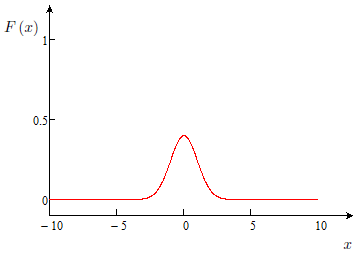
\includegraphics {MHL_DensityOfDistributionOfNormalDistribution_Graph.png}
   \caption{График функции} 
   \label{img:MHL_DensityOfDistributionOfNormalDistribution_Graph}  
 \end{figure}
 



\begin{lstlisting}[label=code_use_MHL_DensityOfDistributionOfNormalDistribution,caption=Пример использования]
        double t;
        double f;
        t=MHL_RandomUniform(0,3);

        //Вызов функции
        f=MHL_DensityOfDistributionOfNormalDistribution(t);

        //Используем полученный результат

        MHL_ShowNumber (t,"Параметр", "t");
        // Параметр:
        //t=1.42401
        MHL_ShowNumber (f,"Значение функции", "f");
        // Значение функции:
        //f=0.144736
\end{lstlisting}

\subsubsection{MHL\_DistributionFunctionOfNormalDistribution}\label{MHL_DistributionFunctionOfNormalDistribution}

Функция распределения нормированного и центрированного нормального распределения.


\begin{lstlisting}[label=code_syntax_MHL_DistributionFunctionOfNormalDistribution,caption=Синтаксис]
double MHL_DistributionFunctionOfNormalDistribution(double x, double Epsilon);
\end{lstlisting}

\textbf{Входные параметры:}

 x --- входная переменная (правая граница интегрирования);
 
 Epsilon --- погрешность (например, Epsilon=0.001).

\textbf{Возвращаемое значение:}

 Значение функции в точке.
 
\textbf{Формула:}
\begin{equation*}
F\left(x \right)=\dfrac{1}{\sqrt{2\pi}}\int_0^x {e^{-\dfrac{x^2}{2}}}.
\end{equation*}

 \begin{figure} [h] 
   \center
   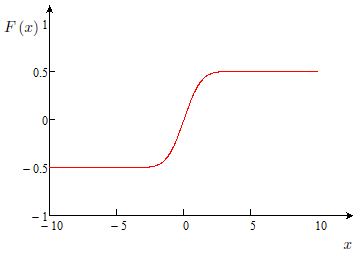
\includegraphics {MHL_DistributionFunctionOfNormalDistribution_Graph.png}
   \caption{График функции} 
   \label{img:MHL_DistributionFunctionOfNormalDistribution_Graph}  
 \end{figure}
 



\begin{lstlisting}[label=code_use_MHL_DistributionFunctionOfNormalDistribution,caption=Пример использования]
        double t;
        double f;
        t=MHL_RandomUniform(0,3);

        //Вызов функции
        f=MHL_DistributionFunctionOfNormalDistribution(t,0.001);

        //Используем полученный результат

        MHL_ShowNumber (t,"Параметр", "t");
        //Параметр:
        //t=2.62253
        MHL_ShowNumber (f,"Значение функции", "f");
        //Значение функции:
        //f=0.495627
\end{lstlisting}

\subsubsection{MHL\_StdDevToVariance}\label{MHL_StdDevToVariance}

Функция переводит среднеквадратичное уклонение в значение дисперсии случайной величины.


\begin{lstlisting}[label=code_syntax_MHL_StdDevToVariance,caption=Синтаксис]
double MHL_StdDevToVariance(double StdDev);
\end{lstlisting}

\textbf{Входные параметры:}

 StdDev --- среднеквадратичное уклонение.

\textbf{Возвращаемое значение:}

 Значение дисперсии случайной величины.



\begin{lstlisting}[label=code_use_MHL_StdDevToVariance,caption=Пример использования]
        double Variance;
        double StdDev=6;

        //Вызов функции
        Variance=MHL_StdDevToVariance(StdDev);

        //Используем результат
        MHL_ShowNumber(Variance,"Дисперсия при среднеквадратичном уклонении, равным "+MHL_NumberToText(StdDev),"равна");
        //Дисперсия при среднеквадратичном уклонении, равным 6:
        //равна=2.44949
\end{lstlisting}

\subsubsection{MHL\_VarianceToStdDev}\label{MHL_VarianceToStdDev}

Функция переводит значение дисперсии случайной величины в среднеквадратичное уклонение.


\begin{lstlisting}[label=code_syntax_MHL_VarianceToStdDev,caption=Синтаксис]
double MHL_VarianceToStdDev(double Variance);
\end{lstlisting}

\textbf{Входные параметры:}

 Variance --- значение дисперсии случайной величины.

\textbf{Возвращаемое значение:}

 Значение среднеквадратичного уклонения.



\begin{lstlisting}[label=code_use_MHL_VarianceToStdDev,caption=Пример использования]
        double StdDev;
        double Variance=6;

        //Вызов функции
        StdDev=MHL_VarianceToStdDev(Variance);

        //Используем полученный результат
        MHL_ShowNumber(StdDev,"Среднеквадратичное уклонение при дисперсии, равной "+MHL_NumberToText(Variance),"равно");
        //Среднеквадратичное уклонение при дисперсии, равной 6:
        //равно=36
\end{lstlisting}

\subsubsection{TMHL\_Mean}\label{TMHL_Mean}

Функция вычисляет среднее арифметическое массива.


\begin{lstlisting}[label=code_syntax_TMHL_Mean,caption=Синтаксис]
template <class T> T TMHL_Mean(T *x, int VMHL_N);
\end{lstlisting}

\textbf{Входные параметры:}

 x --- массив;
 
 VMHL\_N --- размер массива.

\textbf{Возвращаемое значение:}

 Среднее арифметическое массива.



\begin{lstlisting}[label=code_use_TMHL_Mean,caption=Пример использования]
        int i;
        int VMHL_N=10;//Размер массива
        double *a;
        a=new double[VMHL_N];
        //Заполним случайными числами
        for (i=0;i<VMHL_N;i++)
         a[i]=MHL_RandomUniform(0,10);

        //Вызов функции
        double Mean=TMHL_Mean(a,VMHL_N);

        //Используем полученный результат
        MHL_ShowVector (a,VMHL_N,"Массив", "a");
        // Массив:
        //a =
        //4.65149
        //4.00574
        //1.41113
        //1.55457
        //2.75055
        //3.16559
        //8.26508
        //3.86902
        //9.5401
        //4.50836

        MHL_ShowNumber (Mean,"Среднее арифметическое массива", "Mean");
        //Среднее арифметическое массива:
        //Mean=4.37216

        delete [] a;
\end{lstlisting}

\subsubsection{TMHL\_Median}\label{TMHL_Median}

Функция вычисляет медиану выборки.


\begin{lstlisting}[label=code_syntax_TMHL_Median,caption=Синтаксис]
template <class T> T TMHL_Median(T *x, int VMHL_N);
\end{lstlisting}

\textbf{Входные параметры:}

 x --- массив;
 
 VMHL\_N --- размер массива.

\textbf{Возвращаемое значение:}

 Медиана массива.
 
\textbf{ О функции:}

Медиана (50-й процентиль, квантиль 0,5) — возможное значение признака, которое делит ранжированную совокупность (вариационный ряд выборки) на две равные части: 50 % «нижних» единиц ряда данных будут иметь значение признака не больше, чем медиана, а «верхние» 50 % — значения признака не меньше, чем медиана.

В случае, когда число элементов в выборке нечетно, то медиана равна элементу выборки посередине отсортированного массива.

В случае, когда число элементов в выборке четно, то медиана равна среднеарифметическому двух элементов выборки посередине отсортированного массива.



\begin{lstlisting}[label=code_use_TMHL_Median,caption=Пример использования]
        int i;
        int VMHL_N=MHL_RandomUniformInt(3,10);//Размер массива
        double *a;
        a=new double[VMHL_N];
        //Заполним случайными числами
        for (i=0;i<VMHL_N;i++)
         a[i]=MHL_RandomUniform(0,10);

        //Вызов функции
        double Median=TMHL_Median(a,VMHL_N);

        //Используем полученный результат
        MHL_ShowVector (a,VMHL_N,"Массив", "a");
        //Массив:
        //a =
        //8.77167
        //5.89142
        //6.45966
        //3.94775

        MHL_ShowNumber (Median,"Медиана", "Median");
        // Медиана:
        //Median=6.17554

        delete [] a;
\end{lstlisting}

\subsubsection{TMHL\_SampleCovariance}\label{TMHL_SampleCovariance}

Функция вычисляет выборочную ковариацию выборки.


\begin{lstlisting}[label=code_syntax_TMHL_SampleCovariance,caption=Синтаксис]
template <class T> T TMHL_SampleCovariance(T *x, T *y, int VMHL_N);
\end{lstlisting}

\textbf{Входные параметры:}
 
x --- указатель на первую сравниваемую выборки;
 
y --- указатель на вторую сравниваемую выборки;
 
VMHL\_N --- размер массивов.

\textbf{Возвращаемое значение:}
 
Значение выборочной ковариации.

\textbf{Формула:}
\begin{equation*}
Cov\left(\bar{x},\bar{y} \right)= \dfrac{1}{n-1}\sum_{i=1}^{n} \left( x_i-\dfrac{\sum_{j=1}^{n}x_j}{n}\right)\left( y_i-\dfrac{\sum_{j=1}^{n}y_j}{n}\right) .
\end{equation*}



\begin{lstlisting}[label=code_use_TMHL_SampleCovariance,caption=Пример использования]
        int VMHL_N=10;//Размер массива
        double *x;
        x=new double[VMHL_N];
        double *y;
        y=new double[VMHL_N];
        //Заполним случайными числами
        MHL_RandomRealVector (x,0,10,VMHL_N);
        MHL_RandomRealVector (y,0,10,VMHL_N);

        //Вызов функции
        double SampleCovariance=TMHL_SampleCovariance(x,y,VMHL_N);

        //Используем полученный результат
        MHL_ShowVector (x,VMHL_N,"Первый массив", "x");
        // Первый массив:
        //x =
        //3.06915
        //9.92218
        //2.5592
        //9.19586
        //8.23486
        //1.49231
        //3.93158
        //4.97345
        //6.78223
        //1.50909
\end{lstlisting}

\subsubsection{TMHL\_Variance}\label{TMHL_Variance}

Функция вычисляет выборочную дисперсию выборки.


\begin{lstlisting}[label=code_syntax_TMHL_Variance,caption=Синтаксис]
template <class T> T TMHL_Variance(T *x, int VMHL_N);
\end{lstlisting}

\textbf{Входные параметры:}
 
x --- указатель на исходную выборку;
 
VMHL\_N --- размер массива.

\textbf{Возвращаемое значение:}
 
Выборочная дисперсия выборки.


\begin{lstlisting}[label=code_use_TMHL_Variance,caption=Пример использования]
        int VMHL_N=10;//Размер массива
        double *x;
        x=new double[VMHL_N];
        //Заполним случайными числами
        MHL_RandomRealVector (x,0,10,VMHL_N);

        //Вызов функции
        double Variance=TMHL_Variance(x,VMHL_N);

        //Используем полученный результат
        MHL_ShowVector (x,VMHL_N,"Массив", "x");
        //Массив:
        //x =
        //4.61365
        //6.74438
        //0.18219
        //9.68933
        //8.77136
        //2.5177
        //1.89178
        //6.16455
        //8.45978
        //4.33228

        MHL_ShowNumber (Variance,"Значение выборочной дисперсии", "Variance");
        //Значение выборочной дисперсии:
        //Variance=10.1197

        delete [] x;
\end{lstlisting}

\subsection{Тестовые функции для оптимизации}

\subsubsection{MHL\_TestFunction\_Ackley}\label{MHL_TestFunction_Ackley}

Функция многих переменных: Ackley. Тестовая функция вещественной оптимизации.


\begin{lstlisting}[label=code_syntax_MHL_TestFunction_Ackley,caption=Синтаксис]
double MHL_TestFunction_Ackley(double *x, int VMHL_N);
\end{lstlisting}

\textbf{Входные параметры:}

x --- указатель на исходный массив;
 
VMHL\_N --- размер массива x.

\textbf{Возвращаемое значение:} 
 
Значение тестовой функции в точке x.

\textbf {Описание функции}

\begin{tabularwide}
\textbf{Идентификатор:} & MHL\_TestFunction\_Ackley. \\
\textbf{Наименование:} & Функция Ackley. \\
\textbf{Тип:} & Задача вещественной оптимизации. \\
\end{tabularwide}

\textbf{Формула} (целевая функция):
\begin{equation*}
\label{TestFunctions:eq:MHL_TestFunction_Ackley}
f\left( \bar{x}\right) = 20 + e - 20e^{-0.2\sqrt{\frac{1}{n}\sum_{i=1}^{n}\bar{x}_i^2}}-e^{\frac{1}{n}\sqrt{\sum_{i=1}^{n}cos\left( 2\pi\cdot\bar{x}_i\right) }}, \text{ где}
\end{equation*}
\indent $\bar{x}\in X$, $\bar{x}_j\in \left[ Left_j; Right_j\right] $, $Left_j=-5$, $Right_j=5$, $j=\overline{1,n}$.

\begin{tabularwide}
\textbf{Обозначение:} &\specialcell{$\bar{x}$ --- вещественный вектор;\\$n$ --- размерность вещественного вектора.}  \\
\textbf{Решаемая задача оптимизации:} & $\bar{x}_{min}= \arg \min_{\bar{x}\in X} f\left( \bar{x}\right)$.   \\
\textbf{Точка минимума:} & $\bar{x}_{min}={\left( 0,0,\ldots,0\right)}^\mathrm{T} $, то есть $\left(\bar{x}_{min} \right)_j=0$ ($j=\overline{1,n}$).    \\
\textbf{Минимум функции:} & $f\left(\bar{x}_{min} \right) =0$.   \\
\textbf{График:} & Рисунок \ref{TestFunctions:img:MHL_TestFunction_Ackley_Graph} нас \pageref{TestFunctions:img:MHL_TestFunction_Ackley_Graph} стр.   \\
\end{tabularwide}

\begin{figure} [h] 
  \center
  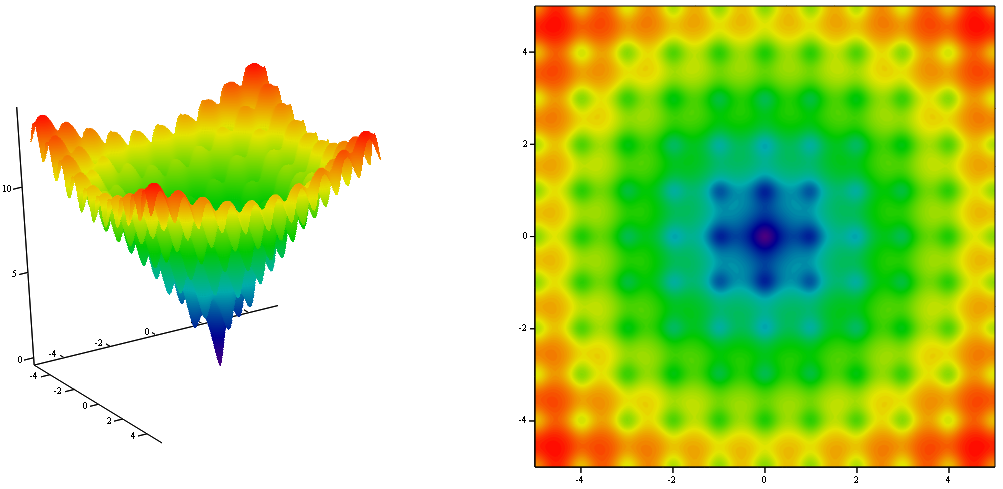
\includegraphics [scale=0.5] {MHL_TestFunction_Ackley_Graph}
  \caption{Функция Ackley} 
  \label{TestFunctions:img:MHL_TestFunction_Ackley_Graph}  
\end{figure}

\textbf {Параметры для алгоритмов оптимизации}

\begin{tabularwide}
\textbf{Точность вычислений:} & $\varepsilon=0.025$. \\
\textbf{Число интервалов, на которые предполагается разбивать каждую компоненту вектора $\bar{x}$ в пределах своего изменения} (для алгоритмов дискретной оптимизации) : & $NumberOfParts_j=4095$ ($j=\overline{1,n}$). \\
\textbf{Для этого длина бинарной строки для $x_j$ координаты равна} (для алгоритмов бинарной оптимизации) : & $\left( k_2\right)_j=12$ ($j=\overline{1,n}$). \\
\end{tabularwide}

\textbf{Замечание:}  $NumberOfParts_j$ выбирается как минимальное число, удовлетворяющее соотношению:
\begin{equation*}
NumberOfParts_j=2^{\left( k_2\right)_j }-1\geq\dfrac{10\left( Right_j-Left_j\right) }{\varepsilon},\text{где } \left( k_2\right)_j \in \mathbb{N}, \left( j=\overline{1,n}\right).
\end{equation*}

\textbf {Основная задача и подзадачи}

\begin{tabularwide}
\textbf{Изменяемый параметр: } & $n$ --- размерность вещественного вектора. \\
\textbf{Значение в основной задаче:} & $n=2$.\\
\textbf{Подзадача №2:} & $n=3$.\\
\textbf{Подзадача №3:} & $n=4$.\\
\textbf{Подзадача №4:} & $n=5$.\\
\textbf{Подзадача №5:} & $n=10$.\\
\textbf{Подзадача №6:} & $n=20$.\\
\textbf{Подзадача №7:} & $n=30$.\\
\end{tabularwide}

\textbf {Нахождение ошибки оптимизации}

Пусть в результате работы алгоритма оптимизации за $N$ запусков мы нашли решения $\bar{x}_{submin}^k$ со значениями целевой функции $f\left( \bar{x}_{submin}^k\right) $ соответственно ($k=\overline{1,N}$). Используем три вида ошибок:

\textbf{Надёжность: }
\begin{equation*}
R = \dfrac{\sum_{k=1}^{N}S\left( \bar{x}_{submin}^k \right) }{N}, \text{ где}
\end{equation*}
\begin{equation*}
S\left( \bar{x}_{submin}^k \right)=\left\lbrace \begin{aligned} 1,& \text{ если } \left| \left( \bar{x}_{submin}^k \right)_j-\left( \bar{x}_{min} \right)_j\right|\leq\varepsilon, j=\overline{1,n};   \\ 0,& \text{ иначе}. \end{aligned}\right.
\end{equation*}

\textbf{Ошибка по входным параметрам:}
\begin{equation*}
E_x = \dfrac{\sum_{k=1}^{N} \left( \frac{\sqrt{\sum_{j=1}^{n}{\left( \left( \bar{x}_{submin}^k \right)_j-\left( \bar{x}_{min} \right)_j \right)}^2 }}{n} \right)  }{N}.
\end{equation*}

\textbf{Ошибка по значениям целевой функции: }
\begin{equation*}
E_f = \dfrac{\sum_{k=1}^{N} \left| f\left( \bar{x}_{submin}^k \right)-f\left( \bar{x}_{min} \right) \right|  }{N}.
\end{equation*}

\textbf {Свойства задачи}

\begin{tabularwide}
\textbf{Условной или безусловной оптимизации: } & Задача безусловной оптимизации. \\
\textbf{Одномерной или многомерной оптимизации: } & Многомерной: $ n $. \\
\textbf{Функция унимодальная или многоэкстремальная: } & Функция многоэкстремальная. \\
\textbf{Функция стохастическая или нет: } & Функция не стохастическая. \\
\textbf{Особенности: } & Нет. \\
\end{tabularwide}


\begin{lstlisting}[label=code_use_MHL_TestFunction_Ackley,caption=Пример использования]
        double *x;
        double f;
        int VMHL_N=2;
        x=new double[VMHL_N];
        for (int i=0;i<VMHL_N;i++) x[i]=MHL_RandomUniform(-5,5);
        f=MHL_TestFunction_Ackley(x,VMHL_N);

        MHL_ShowVector (x,VMHL_N,"Входной вектор", "x");
        //Входной вектор:
        //x =
        //4.51813
        //-4.19861

        MHL_ShowNumber (f,"Значение функции", "f");
        //Значение функции:
        //f=13.645

        delete[] x;
\end{lstlisting}

\subsubsection{MHL\_TestFunction\_ParaboloidOfRevolution}\label{MHL_TestFunction_ParaboloidOfRevolution}

Функция многих переменных: Эллиптический параболоид. Тестовая функция вещественной оптимизации.


\begin{lstlisting}[label=code_syntax_MHL_TestFunction_ParaboloidOfRevolution,caption=Синтаксис]
double MHL_TestFunction_ParaboloidOfRevolution(double *x, int VMHL_N);
\end{lstlisting}

\textbf{Входные параметры:}

x --- указатель на исходный массив;
 
VMHL\_N --- размер массива x.

\textbf{Возвращаемое значение:} 
 
Значение тестовой функции в точке x.

\textbf {Описание функции}

\begin{tabularwide}
\textbf{Идентификатор:} & MHL\_TestFunction\_ParaboloidOfRevolution. \\
\textbf{Наименование:} & Эллиптический параболоид. \\
\textbf{Тип:} & Задача вещественной оптимизации. \\
\end{tabularwide}

\textbf{Формула} (целевая функция):
\begin{equation*}
\label{TestFunctions:eq:MHL_TestFunction_ParaboloidOfRevolution}
f\left( \bar{x}\right) = \sum_{i=1}^{n}\bar{x}_i^2, \text{ где}
\end{equation*}
\indent $\bar{x}\in X$, $\bar{x}_j\in \left[ Left_j; Right_j\right] $, $Left_j=-2$, $Right_j=2$, $j=\overline{1,n}$.

\begin{tabularwide}
\textbf{Обозначение:} &\specialcell{$\bar{x}$ --- вещественный вектор;\\$n$ --- размерность вещественного вектора.}  \\
\textbf{Решаемая задача оптимизации:} & $\bar{x}_{min}= \arg \min_{\bar{x}\in X} f\left( \bar{x}\right)$.   \\
\textbf{Точка минимума:} & $\bar{x}_{min}={\left( 0,0,\ldots,0\right)}^\mathrm{T} $, то есть $\left(\bar{x}_{min} \right)_j=0$ ($j=\overline{1,n}$).    \\
\textbf{Минимум функции:} & $f\left(\bar{x}_{min} \right) =0$.   \\
\textbf{График:} & Рисунок \ref{TestFunctions:img:MHL_TestFunction_ParaboloidOfRevolution_Graph} нас \pageref{TestFunctions:img:MHL_TestFunction_ParaboloidOfRevolution_Graph} стр.   \\
\end{tabularwide}

\begin{figure} [h] 
  \center
  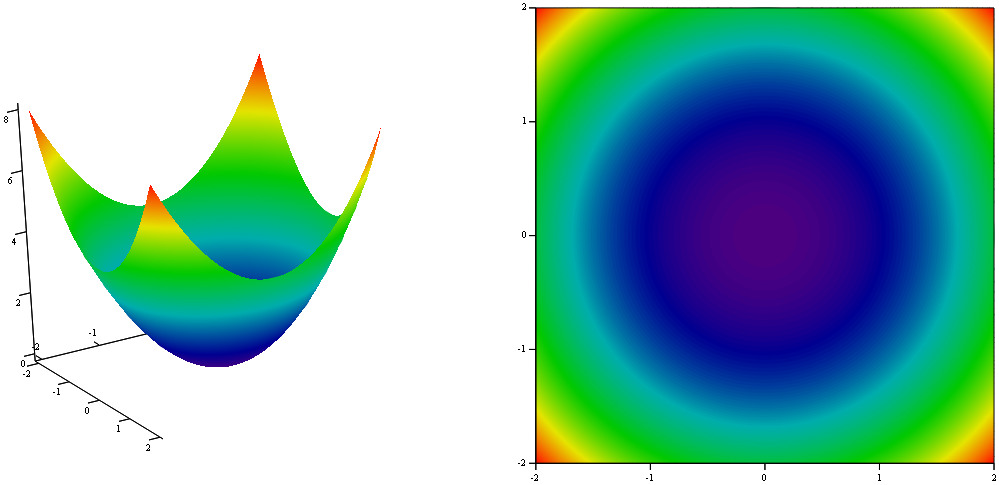
\includegraphics [scale=0.5] {MHL_TestFunction_ParaboloidOfRevolution_Graph}
  \caption{Эллиптический параболоид} 
  \label{TestFunctions:img:MHL_TestFunction_ParaboloidOfRevolution_Graph}  
\end{figure}

\textbf {Параметры для алгоритмов оптимизации}

\begin{tabularwide}
\textbf{Точность вычислений:} & $\varepsilon=0.01$. \\
\textbf{Число интервалов, на которые предполагается разбивать каждую компоненту вектора $\bar{x}$ в пределах своего изменения} (для алгоритмов дискретной оптимизации) : & $NumberOfParts_j=4095$ ($j=\overline{1,n}$). \\
\textbf{Для этого длина бинарной строки для $x_j$ координаты равна} (для алгоритмов бинарной оптимизации) : & $\left( k_2\right)_j=12$ ($j=\overline{1,n}$). \\
\end{tabularwide}

\textbf{Замечание:}  $NumberOfParts_j$ выбирается как минимальное число, удовлетворяющее соотношению:
\begin{equation*}
NumberOfParts_j=2^{\left( k_2\right)_j }-1\geq\dfrac{10\left( Right_j-Left_j\right) }{\varepsilon},\text{где } \left( k_2\right)_j \in \mathbb{N}, \left( j=\overline{1,n}\right).
\end{equation*}

\textbf {Основная задача и подзадачи}

\begin{tabularwide}
\textbf{Изменяемый параметр: } & $n$ --- размерность вещественного вектора. \\
\textbf{Значение в основной задаче:} & $n=2$.\\
\textbf{Подзадача №2:} & $n=3$.\\
\textbf{Подзадача №3:} & $n=4$.\\
\textbf{Подзадача №4:} & $n=5$.\\
\textbf{Подзадача №5:} & $n=10$.\\
\textbf{Подзадача №6:} & $n=20$.\\
\textbf{Подзадача №7:} & $n=30$.\\
\end{tabularwide}

\textbf {Нахождение ошибки оптимизации}

Пусть в результате работы алгоритма оптимизации за $N$ запусков мы нашли решения $\bar{x}_{submin}^k$ со значениями целевой функции $f\left( \bar{x}_{submin}^k\right) $ соответственно ($k=\overline{1,N}$). Используем три вида ошибок:

\textbf{Надёжность: }
\begin{equation*}
R = \dfrac{\sum_{k=1}^{N}S\left( \bar{x}_{submin}^k \right) }{N}, \text{ где}
\end{equation*}
\begin{equation*}
S\left( \bar{x}_{submin}^k \right)=\left\lbrace \begin{aligned} 1,& \text{ если } \left| \left( \bar{x}_{submin}^k \right)_j-\left( \bar{x}_{min} \right)_j\right|\leq\varepsilon, j=\overline{1,n};   \\ 0,& \text{ иначе}. \end{aligned}\right.
\end{equation*}

\textbf{Ошибка по входным параметрам:}
\begin{equation*}
E_x = \dfrac{\sum_{k=1}^{N} \left( \frac{\sqrt{\sum_{j=1}^{n}{\left( \left( \bar{x}_{submin}^k \right)_j-\left( \bar{x}_{min} \right)_j \right)}^2 }}{n} \right)  }{N}.
\end{equation*}

\textbf{Ошибка по значениям целевой функции: }
\begin{equation*}
E_f = \dfrac{\sum_{k=1}^{N} \left| f\left( \bar{x}_{submin}^k \right)-f\left( \bar{x}_{min} \right) \right|  }{N}.
\end{equation*}

\textbf {Свойства задачи}

\begin{tabularwide}
\textbf{Условной или безусловной оптимизации: } & Задача безусловной оптимизации. \\
\textbf{Одномерной или многомерной оптимизации: } & Многомерной: $ n $. \\
\textbf{Функция унимодальная или многоэкстремальная: } & Функция унимодальная. \\
\textbf{Функция стохастическая или нет: } & Функция не стохастическая. \\
\textbf{Особенности: } & Нет. \\
\end{tabularwide}


\begin{lstlisting}[label=code_use_MHL_TestFunction_ParaboloidOfRevolution,caption=Пример использования]
        double *x;
        double f;
        int VMHL_N=2;
        x=new double[VMHL_N];
        for (int i=0;i<VMHL_N;i++) x[i]=MHL_RandomUniform(-2,2);
        f=MHL_TestFunction_ParaboloidOfRevolution(x,VMHL_N);

        MHL_ShowVector (x,VMHL_N,"Входной вектор", "x");
        // Входной вектор:
        //x =
        //0.0842285
        //-1.04395

        MHL_ShowNumber (f,"Значение функции", "f");
        //Значение функции:
        //f=1.09692

        delete[] x;
\end{lstlisting}

\subsubsection{MHL\_TestFunction\_Rastrigin}\label{MHL_TestFunction_Rastrigin}

Функция многих переменных: функция Растригина. Тестовая функция вещественной оптимизации.


\begin{lstlisting}[label=code_syntax_MHL_TestFunction_Rastrigin,caption=Синтаксис]
double MHL_TestFunction_Rastrigin(double *x, int VMHL_N);
\end{lstlisting}

\textbf{Входные параметры:}

x --- указатель на исходный массив;
 
VMHL\_N --- размер массива x.

\textbf{Возвращаемое значение:} 
 
Значение тестовой функции в точке x.

\textbf {Описание функции}

\begin{tabularwide}
\textbf{Идентификатор:} & MHL\_TestFunction\_Rastrigin. \\
\textbf{Наименование:} & Функция Растригина. \\
\textbf{Тип:} & Задача вещественной оптимизации. \\
\end{tabularwide}

\textbf{Формула} (целевая функция):
\begin{equation*}
\label{TestFunctions:eq:MHL_TestFunction_Rastrigin}
f\left( \bar{x}\right) = 10n+\sum_{i=1}^{n}\left( \bar{x}_i^2-10\cdot\cos\left( 2\pi\cdot \bar{x}_i\right) \right) , \text{ где}
\end{equation*}
\indent $\bar{x}\in X$, $\bar{x}_j\in \left[ Left_j; Right_j\right] $, $Left_j=-5$, $Right_j=5$, $j=\overline{1,n}$.

\begin{tabularwide}
\textbf{Обозначение:} &\specialcell{$\bar{x}$ --- вещественный вектор;\\$n$ --- размерность вещественного вектора.}  \\
\textbf{Решаемая задача оптимизации:} & $\bar{x}_{min}= \arg \min_{\bar{x}\in X} f\left( \bar{x}\right)$.   \\
\textbf{Точка минимума:} & $\bar{x}_{min}={\left( 0,0,\ldots,0\right)}^\mathrm{T} $, то есть $\left(\bar{x}_{min} \right)_j=0$ ($j=\overline{1,n}$).    \\
\textbf{Минимум функции:} & $f\left(\bar{x}_{min} \right) =0$.   \\
\textbf{График:} & Рисунок \ref{TestFunctions:img:MHL_TestFunction_Rastrigin_Graph} нас \pageref{TestFunctions:img:MHL_TestFunction_Rastrigin_Graph} стр.   \\
\end{tabularwide}

\begin{figure} [h] 
  \center
  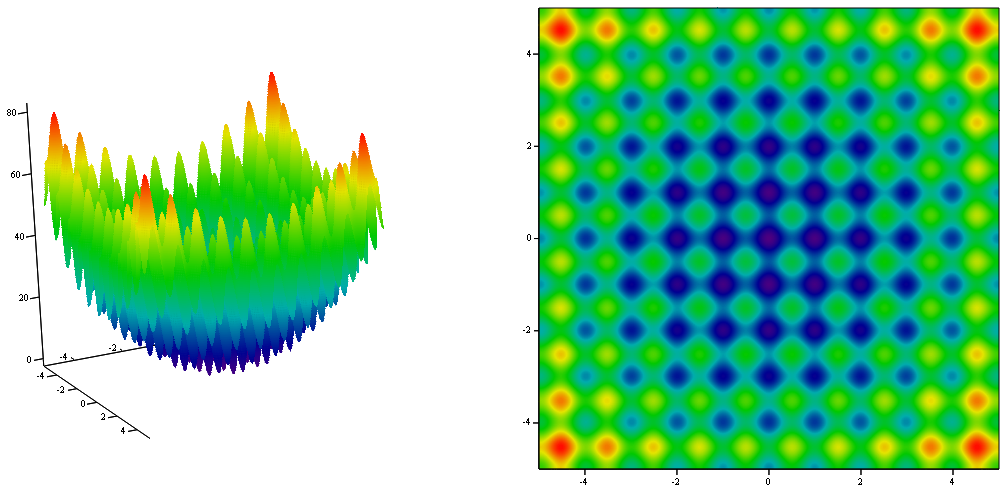
\includegraphics [scale=0.5] {MHL_TestFunction_Rastrigin_Graph}
  \caption{Функция Растригина} 
  \label{TestFunctions:img:MHL_TestFunction_Rastrigin_Graph}  
\end{figure}

\textbf {Параметры для алгоритмов оптимизации}

\begin{tabularwide}
\textbf{Точность вычислений:} & $\varepsilon=0.025$. \\
\textbf{Число интервалов, на которые предполагается разбивать каждую компоненту вектора $\bar{x}$ в пределах своего изменения} (для алгоритмов дискретной оптимизации) : & $NumberOfParts_j=4095$ ($j=\overline{1,n}$). \\
\textbf{Для этого длина бинарной строки для $x_j$ координаты равна} (для алгоритмов бинарной оптимизации) : & $\left( k_2\right)_j=12$ ($j=\overline{1,n}$). \\
\end{tabularwide}

\textbf{Замечание:}  $NumberOfParts_j$ выбирается как минимальное число, удовлетворяющее соотношению:
\begin{equation*}
NumberOfParts_j=2^{\left( k_2\right)_j }-1\geq\dfrac{10\left( Right_j-Left_j\right) }{\varepsilon},\text{где } \left( k_2\right)_j \in \mathbb{N}, \left( j=\overline{1,n}\right).
\end{equation*}

\textbf {Основная задача и подзадачи}

\begin{tabularwide}
\textbf{Изменяемый параметр: } & $n$ --- размерность вещественного вектора. \\
\textbf{Значение в основной задаче:} & $n=2$.\\
\textbf{Подзадача №2:} & $n=3$.\\
\textbf{Подзадача №3:} & $n=4$.\\
\textbf{Подзадача №4:} & $n=5$.\\
\textbf{Подзадача №5:} & $n=10$.\\
\textbf{Подзадача №6:} & $n=20$.\\
\textbf{Подзадача №7:} & $n=30$.\\
\end{tabularwide}

\textbf {Нахождение ошибки оптимизации}

Пусть в результате работы алгоритма оптимизации за $N$ запусков мы нашли решения $\bar{x}_{submin}^k$ со значениями целевой функции $f\left( \bar{x}_{submin}^k\right) $ соответственно ($k=\overline{1,N}$). Используем три вида ошибок:

\textbf{Надёжность: }
\begin{equation*}
R = \dfrac{\sum_{k=1}^{N}S\left( \bar{x}_{submin}^k \right) }{N}, \text{ где}
\end{equation*}
\begin{equation*}
S\left( \bar{x}_{submin}^k \right)=\left\lbrace \begin{aligned} 1,& \text{ если } \left| \left( \bar{x}_{submin}^k \right)_j-\left( \bar{x}_{min} \right)_j\right|\leq\varepsilon, j=\overline{1,n};   \\ 0,& \text{ иначе}. \end{aligned}\right.
\end{equation*}

\textbf{Ошибка по входным параметрам:}
\begin{equation*}
E_x = \dfrac{\sum_{k=1}^{N} \left( \frac{\sqrt{\sum_{j=1}^{n}{\left( \left( \bar{x}_{submin}^k \right)_j-\left( \bar{x}_{min} \right)_j \right)}^2 }}{n} \right)  }{N}.
\end{equation*}

\textbf{Ошибка по значениям целевой функции: }
\begin{equation*}
E_f = \dfrac{\sum_{k=1}^{N} \left| f\left( \bar{x}_{submin}^k \right)-f\left( \bar{x}_{min} \right) \right|  }{N}.
\end{equation*}

\textbf {Свойства задачи}

\begin{tabularwide}
\textbf{Условной или безусловной оптимизации: } & Задача безусловной оптимизации. \\
\textbf{Одномерной или многомерной оптимизации: } & Многомерной: $ n $. \\
\textbf{Функция унимодальная или многоэкстремальная: } & Функция многоэкстремальная. \\
\textbf{Функция стохастическая или нет: } & Функция не стохастическая. \\
\textbf{Особенности: } & Нет. \\
\end{tabularwide}


\begin{lstlisting}[label=code_use_MHL_TestFunction_Rastrigin,caption=Пример использования]
        double *x;
        double f;
        int VMHL_N=2;
        x=new double[VMHL_N];
        for (int i=0;i<VMHL_N;i++) x[i]=MHL_RandomUniform(-5,5);
        f=MHL_TestFunction_Rastrigin(x,VMHL_N);

        MHL_ShowVector (x,VMHL_N,"Входной вектор", "x");
        // Входной вектор:
        //x =
        //2.62268
        //3.52692

        MHL_ShowNumber (f,"Значение функции", "f");
        //Значение функции:
        //f=56.3483

        delete[] x;
\end{lstlisting}

\subsubsection{MHL\_TestFunction\_Rosenbrock}\label{MHL_TestFunction_Rosenbrock}

Функция многих переменных: функция Розенброка. Тестовая функция вещественной оптимизации.


\begin{lstlisting}[label=code_syntax_MHL_TestFunction_Rosenbrock,caption=Синтаксис]
double MHL_TestFunction_Rosenbrock(double *x, int VMHL_N);
\end{lstlisting}

\textbf{Входные параметры:}

x --- указатель на исходный массив;
 
VMHL\_N --- размер массива x.

\textbf{Возвращаемое значение:} 
 
Значение тестовой функции в точке x.

\textbf {Описание функции}

\begin{tabularwide}
\textbf{Идентификатор:} & MHL\_TestFunction\_Rosenbrock. \\
\textbf{Наименование:} & Функция Розенброка. \\
\textbf{Тип:} & Задача вещественной оптимизации. \\
\end{tabularwide}

\textbf{Формула} (целевая функция):
\begin{equation*}
\label{TestFunctions:eq:MHL_TestFunction_Rosenbrock}
f\left( \bar{x}\right) = \sum_{i=1}^{n-1} \left( 100{\left( \bar{x}_{i+1}-\bar{x}_i^2\right)}^2+{\left( 1-\bar{x}_i\right) }^2 \right)  , \text{ где}
\end{equation*}
\indent $\bar{x}\in X$, $\bar{x}_j\in \left[ Left_j; Right_j\right] $, $Left_j=-2$, $Right_j=2$, $j=\overline{1,n}$.

\begin{tabularwide}
\textbf{Обозначение:} &\specialcell{$\bar{x}$ --- вещественный вектор;\\$n$ --- размерность вещественного вектора.}  \\
\textbf{Решаемая задача оптимизации:} & $\bar{x}_{min}= \arg \min_{\bar{x}\in X} f\left( \bar{x}\right)$.   \\
\textbf{Точка минимума:} & $\bar{x}_{min}={\left( 1,1,\ldots,1\right)}^\mathrm{T} $, то есть $\left(\bar{x}_{min} \right)_j=1$ ($j=\overline{1,n}$).    \\
\textbf{Минимум функции:} & $f\left(\bar{x}_{min} \right) =0$.   \\
\textbf{График:} & Рисунок \ref{TestFunctions:img:MHL_TestFunction_Rosenbrock_Graph} нас \pageref{TestFunctions:img:MHL_TestFunction_Rosenbrock_Graph} стр.   \\
\end{tabularwide}

\begin{figure} [h] 
  \center
  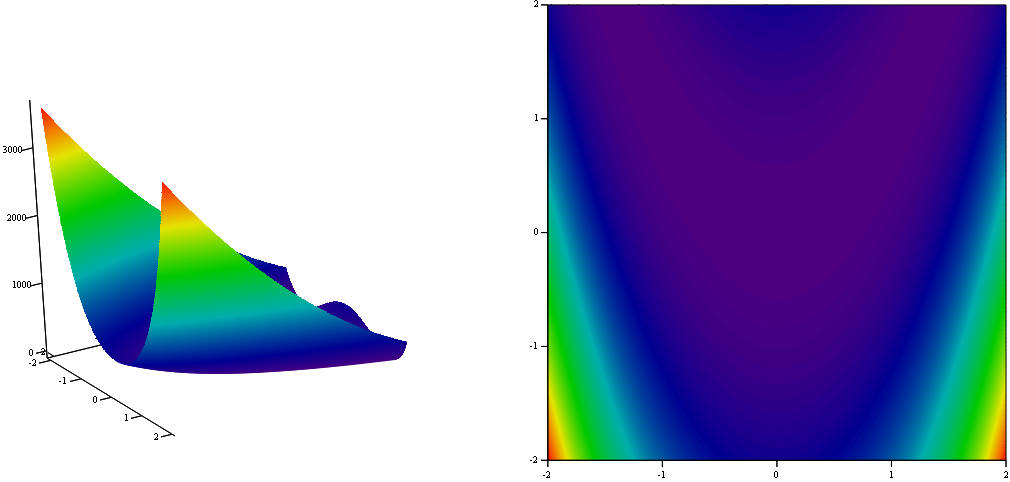
\includegraphics [scale=0.5] {MHL_TestFunction_Rosenbrock_Graph}
  \caption{Функция Розенброка} 
  \label{TestFunctions:img:MHL_TestFunction_Rosenbrock_Graph}  
\end{figure}

\textbf {Параметры для алгоритмов оптимизации}

\begin{tabularwide}
\textbf{Точность вычислений:} & $\varepsilon=0.01$. \\
\textbf{Число интервалов, на которые предполагается разбивать каждую компоненту вектора $\bar{x}$ в пределах своего изменения} (для алгоритмов дискретной оптимизации) : & $NumberOfParts_j=4095$ ($j=\overline{1,n}$). \\
\textbf{Для этого длина бинарной строки для $x_j$ координаты равна} (для алгоритмов бинарной оптимизации) : & $\left( k_2\right)_j=12$ ($j=\overline{1,n}$). \\
\end{tabularwide}

\textbf{Замечание:}  $NumberOfParts_j$ выбирается как минимальное число, удовлетворяющее соотношению:
\begin{equation*}
NumberOfParts_j=2^{\left( k_2\right)_j }-1\geq\dfrac{10\left( Right_j-Left_j\right) }{\varepsilon},\text{где } \left( k_2\right)_j \in \mathbb{N}, \left( j=\overline{1,n}\right).
\end{equation*}

\textbf {Основная задача и подзадачи}

\begin{tabularwide}
\textbf{Изменяемый параметр: } & $n$ --- размерность вещественного вектора. \\
\textbf{Значение в основной задаче:} & $n=2$.\\
\textbf{Подзадача №2:} & $n=3$.\\
\textbf{Подзадача №3:} & $n=4$.\\
\textbf{Подзадача №4:} & $n=5$.\\
\textbf{Подзадача №5:} & $n=10$.\\
\textbf{Подзадача №6:} & $n=20$.\\
\textbf{Подзадача №7:} & $n=30$.\\
\end{tabularwide}

\textbf {Нахождение ошибки оптимизации}

Пусть в результате работы алгоритма оптимизации за $N$ запусков мы нашли решения $\bar{x}_{submin}^k$ со значениями целевой функции $f\left( \bar{x}_{submin}^k\right) $ соответственно ($k=\overline{1,N}$). Используем три вида ошибок:

\textbf{Надёжность: }
\begin{equation*}
R = \dfrac{\sum_{k=1}^{N}S\left( \bar{x}_{submin}^k \right) }{N}, \text{ где}
\end{equation*}
\begin{equation*}
S\left( \bar{x}_{submin}^k \right)=\left\lbrace \begin{aligned} 1,& \text{ если } \left| \left( \bar{x}_{submin}^k \right)_j-\left( \bar{x}_{min} \right)_j\right|\leq\varepsilon, j=\overline{1,n};   \\ 0,& \text{ иначе}. \end{aligned}\right.
\end{equation*}

\textbf{Ошибка по входным параметрам:}
\begin{equation*}
E_x = \dfrac{\sum_{k=1}^{N} \left( \frac{\sqrt{\sum_{j=1}^{n}{\left( \left( \bar{x}_{submin}^k \right)_j-\left( \bar{x}_{min} \right)_j \right)}^2 }}{n} \right)  }{N}.
\end{equation*}

\textbf{Ошибка по значениям целевой функции: }
\begin{equation*}
E_f = \dfrac{\sum_{k=1}^{N} \left| f\left( \bar{x}_{submin}^k \right)-f\left( \bar{x}_{min} \right) \right|  }{N}.
\end{equation*}

\textbf {Свойства задачи}

\begin{tabularwide}
\textbf{Условной или безусловной оптимизации: } & Задача безусловной оптимизации. \\
\textbf{Одномерной или многомерной оптимизации: } & Многомерной: $ n $. \\
\textbf{Функция унимодальная или многоэкстремальная: } & Функция многоэкстремальная. \\
\textbf{Функция стохастическая или нет: } & Функция не стохастическая. \\
\textbf{Особенности: } & Нет. \\
\end{tabularwide}


\begin{lstlisting}[label=code_use_MHL_TestFunction_Rosenbrock,caption=Пример использования]
        double *x;
        double f;
        int VMHL_N=2;
        x=new double[VMHL_N];
        for (int i=0;i<VMHL_N;i++) x[i]=MHL_RandomUniform(-2,2);
        f=MHL_TestFunction_Rosenbrock(x,VMHL_N);

        MHL_ShowVector (x,VMHL_N,"Входной вектор", "x");
        // Входной вектор:
        //x =
        //-1.28491
        //0.342896


        MHL_ShowNumber (f,"Значение функции", "f");
        //Значение функции:
        //f=176.334

        delete[] x;
\end{lstlisting}

\subsubsection{MHL\_TestFunction\_SumVector}\label{MHL_TestFunction_SumVector}

Сумма всех элементов бинарного вектора. Тестовая функция бинарной оптимизации.


\begin{lstlisting}[label=code_syntax_MHL_TestFunction_SumVector,caption=Синтаксис]
double MHL_TestFunction_SumVector(int *x, int VMHL_N);
\end{lstlisting}

\textbf{Входные параметры:}

x --- указатель на исходный массив;
 
VMHL\_N --- размер массива x.

\textbf{Возвращаемое значение:} 
 
Значение тестовой функции в точке x.

\textbf {Описание функции}

\begin{tabularwide}
\textbf{Идентификатор:} & MHL\_TestFunction\_SumVector. \\
\textbf{Наименование:} & Сумма всех элементов бинарного вектора. \\
\textbf{Тип:} & Задача бинарной оптимизации. \\
\end{tabularwide}

\textbf{Формула} (целевая функция):
\begin{equation*}
\label{TestFunctions:eq:MHL_TestFunction_SumVector}
f\left( \bar{x}\right) = \sum_{i=1}^{n}\bar{x}_i, \text{ где}
\end{equation*}
\indent $\bar{x}\in X$, $\bar{x}_j\in \left\lbrace 0; 1 \right\rbrace  $, $j=\overline{1,n}$.

\begin{tabularwide}
\textbf{Обозначение:} &\specialcell{$\bar{x}$ --- бинарный вектор;\\$n$ --- размерность бинарного вектора.}  \\
\textbf{Объем поискового пространства:} & $\mu\left( X\right)=2^n $.   \\
\textbf{Решаемая задача оптимизации:} & $\bar{x}_{max}= \arg \max_{\bar{x}\in X} f\left( \bar{x}\right)$.   \\
\textbf{Точка максимума:} & $\bar{x}_{max}={\left( 1,1,\ldots,1\right)}^\mathrm{T} $, то есть $\left(\bar{x}_{max} \right)_j=1$ ($j=\overline{1,n}$).    \\
\textbf{Максимум функции:} & $f\left(\bar{x}_{max} \right) =n$.   \\
\textbf{Точка минимума:} & $\bar{x}_{min}={\left( 0,0,\ldots,0\right)}^\mathrm{T} $, то есть $\left(\bar{x}_{min} \right)_j=0$ ($j=\overline{1,n}$).    \\
\textbf{Минимум функции:} & $f\left(\bar{x}_{min} \right) =0$.   \\
\end{tabularwide}

\textbf {Основная задача и подзадачи}

\begin{tabularwide}
\textbf{Изменяемый параметр: } & $n$ --- размерность бинарного вектора. \\
\textbf{Значение в основной задаче:} & $n=20$.\\
\textbf{Подзадача №2:} & $n=30$.\\
\textbf{Подзадача №3:} & $n=40$.\\
\textbf{Подзадача №4:} & $n=50$.\\
\textbf{Подзадача №5:} & $n=60$.\\
\textbf{Подзадача №6:} & $n=70$.\\
\textbf{Подзадача №7:} & $n=80$.\\
\textbf{Подзадача №8:} & $n=90$.\\
\textbf{Подзадача №9:} & $n=100$.\\
\textbf{Подзадача №10:} & $n=200$.\\
\end{tabularwide}

\textbf {Нахождение ошибки оптимизации}

Пусть в результате работы алгоритма оптимизации за $N$ запусков мы нашли решения $\bar{x}_{submax}^k$ со значениями целевой функции $f\left( \bar{x}_{submax}^k\right) $ соответственно ($k=\overline{1,N}$). Используем три вида ошибок:

\textbf{Надёжность: }
\begin{equation*}
R = \dfrac{\sum_{k=1}^{N}S\left( \bar{x}_{submax}^k \right) }{N}, \text{ где}
\end{equation*}
\begin{equation*}
S\left( \bar{x}_{submax}^k \right)=\left\lbrace \begin{aligned} 1,& \text{ если } \bar{x}_{submax}^k = \bar{x}_{max} ;   \\ 0,& \text{ иначе}. \end{aligned}\right.
\end{equation*}

\textbf{Ошибка по входным параметрам:}
\begin{equation*}
E_x = \dfrac{\sum_{k=1}^{N} \left( \frac{\sum_{j=1}^{n}\left| \left( \bar{x}_{submax}^k \right)_j-\left( \bar{x}_{max} \right)_j \right| }{n} \right)  }{N}.
\end{equation*}

\textbf{Ошибка по значениям целевой функции: }
\begin{equation*}
E_f = \dfrac{\sum_{k=1}^{N} \left| f\left( \bar{x}_{submax}^k \right)-f\left( \bar{x}_{max} \right) \right|  }{N}.
\end{equation*}

\textbf {Свойства задачи}

\begin{tabularwide}
\textbf{Условной или безусловной оптимизации: } & Задача безусловной оптимизации. \\
\textbf{Одномерной или многомерной оптимизации: } & Многомерной: $ n $. \\
\textbf{Функция унимодальная или многоэкстремальная: } & Функция унимодальная. \\
\textbf{Функция стохастическая или нет: } & Функция не стохастическая. \\
\textbf{Особенности: } & Нет. \\
\end{tabularwide}


\begin{lstlisting}[label=code_use_MHL_TestFunction_SumVector,caption=Пример использования]
        int VMHL_N=10;//Размер массива (число строк)
        int *x;
        x=new int[VMHL_N];
        //Получим случайный бинарный вектор
        TMHL_RandomBinaryVector(x,VMHL_N);

        //Вызов функции
        double f=MHL_TestFunction_SumVector(x,VMHL_N);

        //Используем полученный результат
        MHL_ShowVector (x,VMHL_N,"Вектор", "x");
        //Вектор:
        //x =	
        //0
        //0
        //1
        //0
        //0
        //1
        //1
        //1
        //0
        //1
        
        MHL_ShowNumber (f,"Значение функции в точке", "f");
        //Значение функции в точке:
        //f=5
                
        delete [] x;
\end{lstlisting}

\subsection{Тригонометрические функции}

\subsubsection{MHL\_Cos}\label{MHL_Cos}

Функция возвращает косинус угла в радианах.


\begin{lstlisting}[label=code_syntax_MHL_Cos,caption=Синтаксис]
double MHL_Cos(double x);
\end{lstlisting}

\textbf{Входные параметры:}

 x --- угол в радианах.

\textbf{Возвращаемое значение:}

Косинус угла.

\textbf{Примечание:}

Вводится только для того, чтобы множество тригонометрических функций было полным.


\begin{lstlisting}[label=code_use_MHL_Cos,caption=Пример использования]
        double y;
        double Angle=MHL_PI;//Угол в радинах

        //Вызов функции
        y=MHL_Cos(Angle);

        //Используем полученный результат
        MHL_ShowNumber(y,"Косинус угла "+MHL_NumberToText(Angle)+" радианов","равен");
        //Косинус угла 3.14159 радианов:
        //равен=-1
\end{lstlisting}

\subsubsection{MHL\_CosDeg}\label{MHL_CosDeg}

Функция возвращает косинус угла в градусах.


\begin{lstlisting}[label=code_syntax_MHL_CosDeg,caption=Синтаксис]
double MHL_CosDeg(double x);
\end{lstlisting}

\textbf{Входные параметры:}

 x --- угол в градусах.

\textbf{Возвращаемое значение:}

Косинус угла.


\begin{lstlisting}[label=code_use_MHL_CosDeg,caption=Пример использования]
        double y;
        double Angle=180;//Угол в градусах

        //Вызов функции
        y=MHL_CosDeg(Angle);

        //Используем полученный результат
        MHL_ShowNumber(y,"Косинус угла "+MHL_NumberToText(Angle)+" градусов","равен");
        //Косинус угла 180 градусов:
        //равен=-1
\end{lstlisting}

\subsubsection{MHL\_Cosec}\label{MHL_Cosec}

Функция возвращает косеканс угла в радианах.


\begin{lstlisting}[label=code_syntax_MHL_Cosec,caption=Синтаксис]
double MHL_Cosec(double x);
\end{lstlisting}

\textbf{Входные параметры:}

 x --- угол в радианах.

\textbf{Возвращаемое значение:}

Косеканс угла.


\begin{lstlisting}[label=code_use_MHL_Cosec,caption=Пример использования]
        double y;
        double Angle=MHL_PI/4.;//Угол в радинах

        //Вызов функции
        y=MHL_Cosec(Angle);

        //Используем полученный результат
        MHL_ShowNumber(y,"Косеканс угла "+MHL_NumberToText(Angle)+" радианов","равен");
        //Косеканс угла 0.785398 радианов:
        //равен=1.41421
\end{lstlisting}

\subsubsection{MHL\_CosecDeg}\label{MHL_CosecDeg}

Функция возвращает косеканс угла в градусах.


\begin{lstlisting}[label=code_syntax_MHL_CosecDeg,caption=Синтаксис]
double MHL_CosecDeg(double x);
\end{lstlisting}

\textbf{Входные параметры:}

 x --- угол в градусах.

\textbf{Возвращаемое значение:}

Косеканс угла.


\begin{lstlisting}[label=code_use_MHL_CosecDeg,caption=Пример использования]
        double y;
        double Angle=45;//Угол в градусах

        //Вызов функции
        y=MHL_CosecDeg(Angle);

        //Используем полученный результат
        MHL_ShowNumber(y,"Косеканс угла "+MHL_NumberToText(Angle)+" градусов","равен");
        //Косеканс угла 45 градусов:
        //равен=1.41421
\end{lstlisting}

\subsubsection{MHL\_Cotan}\label{MHL_Cotan}

Функция возвращает котангенс угла в радианах.


\begin{lstlisting}[label=code_syntax_MHL_Cotan,caption=Синтаксис]
double MHL_Cotan(double x);
\end{lstlisting}

\textbf{Входные параметры:}

 x --- угол в радианах.

\textbf{Возвращаемое значение:}

Котангенс угла.


\begin{lstlisting}[label=code_use_MHL_Cotan,caption=Пример использования]
        double y;
        double Angle=MHL_PI/4.;//Угол в радинах

        //Вызов функции
        y=MHL_Cotan(Angle);

        //Используем полученный результат
        MHL_ShowNumber(y,"Котангенс угла "+MHL_NumberToText(Angle)+" радианов","равен");
        //Котангенс угла 0.785398 радианов:
        //равен=1
\end{lstlisting}

\subsubsection{MHL\_CotanDeg}\label{MHL_CotanDeg}

Функция возвращает котангенс угла в градусах.


\begin{lstlisting}[label=code_syntax_MHL_CotanDeg,caption=Синтаксис]
double MHL_CotanDeg(double x);
\end{lstlisting}

\textbf{Входные параметры:}

 x --- угол в градусах.

\textbf{Возвращаемое значение:}

Котангенс угла.


\begin{lstlisting}[label=code_use_MHL_CotanDeg,caption=Пример использования]
        double y;
        double Angle=45;//Угол в градусах

        //Вызов функции
        y=MHL_CotanDeg(Angle);

        //Используем полученный результат
        MHL_ShowNumber(y,"Котангенс угла "+MHL_NumberToText(Angle)+" градусов","равен");
        //Котангенс угла 45 градусов:
        //равен=1
\end{lstlisting}

\subsubsection{MHL\_Sec}\label{MHL_Sec}

Функция возвращает секанс угла в радианах.


\begin{lstlisting}[label=code_syntax_MHL_Sec,caption=Синтаксис]
double MHL_Sec(double x);
\end{lstlisting}

\textbf{Входные параметры:}

 x --- угол в радианах.

\textbf{Возвращаемое значение:}

Секанс угла.


\begin{lstlisting}[label=code_use_MHL_Sec,caption=Пример использования]
        double y;
        double Angle=MHL_PI/4.;//Угол в радинах

        //Вызов функции
        y=MHL_Sec(Angle);

        //Используем полученный результат
        MHL_ShowNumber(y,"Секанс угла "+MHL_NumberToText(Angle)+" радианов","равен");
        //Секанс угла 0.785398 радианов:
        //равен=1.41421
\end{lstlisting}

\subsubsection{MHL\_SecDeg}\label{MHL_SecDeg}

Функция возвращает секанс угла в градусах.


\begin{lstlisting}[label=code_syntax_MHL_SecDeg,caption=Синтаксис]
double MHL_SecDeg(double x);
\end{lstlisting}

\textbf{Входные параметры:}

 x --- угол в градусах.

\textbf{Возвращаемое значение:}

Секанс угла.


\begin{lstlisting}[label=code_use_MHL_SecDeg,caption=Пример использования]
        double y;
        double Angle=45;//Угол в градусах

        //Вызов функции
        y=MHL_SecDeg(Angle);

        //Используем полученный результат
        MHL_ShowNumber(y,"Секанс угла "+MHL_NumberToText(Angle)+" градусов","равен");
        //Секанс угла 45 градусов:
        //равен=1.41421
\end{lstlisting}

\subsubsection{MHL\_Sin}\label{MHL_Sin}

Функция возвращает синус угла в радианах.


\begin{lstlisting}[label=code_syntax_MHL_Sin,caption=Синтаксис]
double MHL_Sin(double x);
\end{lstlisting}

\textbf{Входные параметры:}

 x --- угол в радианах.

\textbf{Возвращаемое значение:}

Синус угла.

\textbf{Примечание:}

 Вводится только для того, чтобы множество тригонометрических функций было полным.


\begin{lstlisting}[label=code_use_MHL_Sin,caption=Пример использования]
        double y;
        double Angle=MHL_PI/2.;//Угол в радинах

        //Вызов функции
        y=MHL_Sin(Angle);

        //Используем полученный результат
        MHL_ShowNumber(y,"Синус угла "+MHL_NumberToText(Angle)+" радианов","равен");
        //Синус угла 1.5708 радианов:
        //равен=1
\end{lstlisting}

\subsubsection{MHL\_SinDeg}\label{MHL_SinDeg}

Функция возвращает синус угла в градусах.


\begin{lstlisting}[label=code_syntax_MHL_SinDeg,caption=Синтаксис]
double MHL_SinDeg(double x);
\end{lstlisting}

\textbf{Входные параметры:}

 x --- угол в градусах.

\textbf{Возвращаемое значение:}

Синус угла.


\begin{lstlisting}[label=code_use_MHL_SinDeg,caption=Пример использования]
        double y;
        double Angle=90;//Угол в градусах

        //Вызов функции
        y=MHL_SinDeg(Angle);

        //Используем полученный результат
        MHL_ShowNumber(y,"Синус угла "+MHL_NumberToText(Angle)+" градусов","равен");
        //Синус угла 90 градусов:
        //равен=1
\end{lstlisting}

\subsubsection{MHL\_Tan}\label{MHL_Tan}

Функция возвращает тангенс угла в радианах.


\begin{lstlisting}[label=code_syntax_MHL_Tan,caption=Синтаксис]
double MHL_Tan(double x);
\end{lstlisting}

\textbf{Входные параметры:}

 x --- угол в радианах.

\textbf{Возвращаемое значение:}

Тангенс угла.

\textbf{Примечание:}

 Вводится только для того, чтобы множество тригонометрических функций было полным.


\begin{lstlisting}[label=code_use_MHL_Tan,caption=Пример использования]
        double y;
        double Angle=MHL_PI/4.;//Угол в радинах

        //Вызов функции
        y=MHL_Tan(Angle);

        //Используем полученный результат
        MHL_ShowNumber(y,"Тангенс угла "+MHL_NumberToText(Angle)+" радианов","равен");
        //Тангенс угла 0.785398 радианов:
        //равен=1
\end{lstlisting}

\subsubsection{MHL\_TanDeg}\label{MHL_TanDeg}

Функция возвращает тангенс угла в градусах.


\begin{lstlisting}[label=code_syntax_MHL_TanDeg,caption=Синтаксис]
double MHL_TanDeg(double x);
\end{lstlisting}

\textbf{Входные параметры:}

 x --- угол в градусах.

\textbf{Возвращаемое значение:}

Тангенс угла.


\begin{lstlisting}[label=code_use_MHL_TanDeg,caption=Пример использования]
        double y;
        double Angle=45;//Угол в градусах

        //Вызов функции
        y=MHL_TanDeg(Angle);

        //Используем полученный результат
        MHL_ShowNumber(y,"Тангенс угла "+MHL_NumberToText(Angle)+" градусов","равен");
        //Тангенс угла 45 градусов:
        //равен=1
\end{lstlisting}

\subsection{Уравнения}

\subsubsection{MHL\_QuadraticEquation}\label{MHL_QuadraticEquation}

Функция решает квадратное уравнение вида: $a\cdot x^2+b\cdot x+c=0$. Ответ представляет собой два действительных числа.


\begin{lstlisting}[label=code_syntax_MHL_QuadraticEquation,caption=Синтаксис]
int MHL_QuadraticEquation(double a, double b, double c, double *x1, double *x2);
\end{lstlisting}

\textbf{Входные параметры:}
 
a --- параметр уравнения;
 
b --- параметр уравнения;
 
c --- параметр уравнения;
 
x1 --- первый корень;
 
x2 --- второй корень.

\textbf{Возвращаемое значение:}
 
1 --- все хорошо;
 
0 --- дискриминант отрицательный.



\begin{lstlisting}[label=code_use_MHL_QuadraticEquation,caption=Пример использования]
        double a=MHL_RandomUniformInt(1,10);
        double b=MHL_RandomUniformInt(1,10);
        double c=MHL_RandomUniformInt(1,10);
        double x1;
        double x2;

        int Result=MHL_QuadraticEquation(a,b,c,&x1,&x2);;

        //Используем полученный результат
        MHL_ShowText("Квадратное уравнение: "+MHL_NumberToText(a)+"x^2+"+MHL_NumberToText(b)+"x+"+MHL_NumberToText(c)+"=0");
        //Квадратное уравнение: 1x^2+8x+5:
        MHL_ShowNumber(Result,"Найдено ли решение","Result");
        //Найдено ли решение:
        //Result=1
        if (Result==1)
        {
        MHL_ShowNumber(x1,"Первый корень квадратного уравнения","x1");
        //Первый корень квадратного уравнения:
        //x1=-0.683375
        MHL_ShowNumber(x2,"Первый корень квадратного уравнения","x2");
        //Первый корень квадратного уравнения:
        //x2=-7.31662
        }
\end{lstlisting}

\newpage

\end{document}